 %% ----------------------------------------------------------------
%% Thesis.tex -- MAIN FILE (the one that you compile with LaTeX)
%% ---------------------------------------------------------------- 

% Set up the document
\documentclass[a4paper, 11pt, oneside]{Thesis}  % Use the "Thesis" style, based on the ECS Thesis style by Steve Gunn
\graphicspath{{Figures/}}  % Location of the graphics files (set up for graphics to be in PDF format)

% Include any extra LaTeX packages required
\usepackage[square, numbers, comma, sort&compress]{natbib} 	 % Use the "Natbib" style for the references in the Bibliography
\usepackage{verbatim}  % Needed for the "comment" environment to make LaTeX comments
\usepackage{vector}  % Allows "\bvec{}" and "\buvec{}" for "blackboard" style bold vectors in maths
\hypersetup{urlcolor=blue, colorlinks=true}  % Colours hyperlinks in blue, but this can be distracting if there are many links.
%\usepackage[ruled]{algorithm2e}
%\renewcommand{\algorithmcfname}{ALGORITHM}
% Langue
\usepackage[T1]{fontenc}
\usepackage[mac]{inputenc}
\usepackage[frenchb,english]{babel} % On peut aussi mettre english ici.
% Figures et couleurs
\usepackage{graphicx}
\usepackage{subfigure}
\usepackage{color}
\definecolor{gris}{gray}{0.45}
\usepackage{appendix}
\usepackage{MnSymbol}
\usepackage{multirow}
\usepackage{listings}
\usepackage{algorithm}
\usepackage{algpseudocode}
% Font math
\usepackage{hyperref}
\usepackage{amssymb, amsmath, amsfonts} 
\usepackage{dsfont}
% Mise en page latex et police
\usepackage{vmargin}
\usepackage{tikz-timing}[2009/05/15]
\usepackage{tikz}
\usetikzlibrary{shapes,arrows,shadows}
\usepackage{verbatim}
\usetikzlibrary[patterns]
\usepackage[underline=true,rounded corners=false]{pgf-umlsd}
\usepackage{setspace}
\usepackage{enumerate}
\usepackage{hhline}
%\doublespace
%\setlength{\parskip}{2cm}
%\setlength{\baselineskip}{2cm plus 0pt minus 0pt}
\usepackage{pdfpages}

% New command
\newcommand{\maxdmin}{\mbox{$\max\!\text{-}d_{\min}$}}
\newcommand{\maxlmin}{\mbox{$\max\!\text{-}\lambda_{\min}$}}
\newcommand{\dmin}{$d_{\min}$}

\DeclareMathOperator*{\argmax}{arg\,max}
\DeclareMathOperator*{\argmin}{arg\,min}
\DeclareMathOperator{\cotan}{cotan}
\DeclareMathOperator{\atan}{atan}
\DeclareMathOperator{\rank}{rank}
\DeclareMathOperator{\diag}{diag}
\DeclareMathOperator{\trace}{trace}

\newcommand{\blankspace}{\clearpage
\thispagestyle{empty}
\phantom{a}
\vfill
\newpage
\vfill
\addtocounter{page}{-1}} 

%% ----------------------------------------------------------------
\begin{document}
%\setlength{\baselineskip}{2cm plus 0pt minus 0pt}

%\newlength{\plarg}
%\setlength{\plarg}{8cm}
%\newlength{\glarg}
%\setlength{\glarg}{14cm}
%\newlength{\Glarg}
%\setlength{\Glarg}{15cm}
%



\includepdf[offset= 80 -80]{./chapters/coverpage.pdf}



%\blankspace
\frontmatter	  % Begin Roman style (i, ii, iii, iv...) page numbering

\setcounter{page}{1}
\pagenumbering{Roman}

% Set up the Title Page
\title  {SmartSense}
\authors  {\texorpdfstring
            {\href{xuan-chien.le@irisa.fr}{Xuan-Chien LE}}
            {Xuan-Chien LE}
            }
\addresses  {\groupname\\\deptname\\\univname}  % Do not change this here, instead these must be set in the "Thesis.cls" file, please look through it instead
\date   {\today}
\subject    {}
\keywords   {}

%\maketitle
% ----------------------------------------------------------------

\setstretch{1.3}  % It is better to have smaller font and larger line spacing than the other way round

% Define the page headers using the FancyHdr package and set up for one-sided printing
\fancyhead{}  % Clears all page headers and footers
\rhead{\thepage}  % Sets the right side header to show the page number
\lhead{}  % Clears the left side page header

\pagestyle{fancy}  % Finally, use the "fancy" page style to implement the FancyHdr headers

% ----------------------------------------------------------------
% Declaration Page required for the Thesis, your institution may give you a different text to place here
%\Declaration{
%
%\addtocontents{toc}{\vspace{1em}}  % Add a gap in the Contents, for aesthetics
%
%I,Quoc-Tuong NGO, declare that this thesis titled, `Generalized Minimum Distance Based Precoders 
%for MIMO Spatial Multiplexing Systems' and the work presented in it are my own. I confirm that:
%
%\begin{itemize} 
%\item[\tiny{$\blacksquare$}] This work was done wholly or mainly while in candidature for a research degree at this University.
% 
%\item[\tiny{$\blacksquare$}] Where any part of this thesis has previously been submitted for a degree or any other qualification at this University or any other institution, this has been clearly stated.
% 
%\item[\tiny{$\blacksquare$}] Where I have consulted the published work of others, this is always clearly attributed.
% 
%\item[\tiny{$\blacksquare$}] Where I have quoted from the work of others, the source is always given. With the exception of such quotations, this thesis is entirely my own work.
% 
%\item[\tiny{$\blacksquare$}] I have acknowledged all main sources of help.
% 
%\item[\tiny{$\blacksquare$}] Where the thesis is based on work done by myself jointly with others, I have made clear exactly what was done by others and what I have contributed myself.
%\\
%\end{itemize}
% 
% 
%Signed:\\
%\rule[1em]{25em}{0.5pt}  % This prints a line for the signature
% 
%Date:\\
%\rule[1em]{25em}{0.5pt}  % This prints a line to write the date
%}
%\clearpage  % Declaration ended, now start a new page







%% ----------------------------------------------------------------
% The "Funny Quote Page"
\pagestyle{empty}  % No headers or footers for the following pages

\null\vfill
% Now comes the "Funny Quote", written in italics
\textit{"Nothing is impossible, the word itself says 'I'm possible'!"}

\begin{flushright}
--- Audrey Hepburn
\end{flushright}

\vfill\vfill\vfill\vfill\vfill\vfill\null
\clearpage  % Funny Quote page ended, start a new page
%%% ----------------------------------------------------------------
%% The Abstract Page
%\addtotoc{Abstract}  % Add the "Abstract" page entry to the Contents
%\abstract{
%\addtocontents{toc}{\vspace{1em}}  % Add a gap in the Contents, for aesthetics
%
%%The Thesis Abstract is written here (and usually kept to just this page). The page is kept centered vertically so can expand into the blank space above the title too\ldots
%}

%\clearpage  % Abstract ended, start a new page
%% ----------------------------------------------------------------




%\blankspace

\setstretch{1.3}  % Reset the line-spacing to 1.3 for body text (if it has changed)
\setcounter{page}{1}
\pagenumbering{roman}

% The Acknowledgements page, for thanking everyone
%\acknowledgements{

More than three years working in this thesis is the most memorial period in my life. It is an honor for me to work and study in a dynamic laboratory, CAIRN in Lannion. 

Firstly, I grateful thank my supervisor Oliver Sentieys, the head of CAIRN, and co-supervisor Baptiste Vrigneau for their consistent supervision and encouragement throughout my study and research, their patient guidance on direction of my work. They gave me breakthrough ideas to improve my works. All of their feedback and suggestions at various stages have been significantly improved my knowledge, scientific minds, and skills of writing and presentation. Besides, I would like to thank Arnaud Carer for his supports in sensor network deployment. 

Secondly, I would like to thank all of my friends in Lannion for their sharing and help. This helps me alleviate homesickness and focus on my work.

My warmest thanks also go to my parents and my younger sister for their never ending support. They always assist me in implementing my desires. 

Finally, I would like to say something special to my wife. She is a powerful emotional support that I can share my burdens and sadness. Thank you for her understanding, her help and her endless love.

The work presented in this thesis is supported by the European Union through the European Regional Development Fund (ERDF), and by the French region of Brittany and INRIA.
}

\clearpage  % End of the Acknowledgements
%% ----------------------------------------------------------------
%\blankspace

\pagestyle{fancy}  %The page style headers have been "empty" all this time, now use the "fancy" headers as defined before to bring them back

%% ----------------------------------------------------------------
\lhead{\emph{Contents}}  % Set the left side page header to "Contents"
\tableofcontents  % Write out the Table of Contents

%% ----------------------------------------------------------------
%\lhead{\emph{Abbreviations}}  % Set the left side page header to "Abbreviations"
%\input{Abbreviations}

% ----------------------------------------------------------------
\lhead{\emph{List of Acronyms}}  % Set the left side page header to "Abbreviations"
\listofsymbols{ll}  % Include a list of Abbreviations (a table of two columns)
{
ANN & Artificial Neural Network\\
BiRNN & Bidirectional Recurrent Neural Network layer\\
BLUED & Building-Level fUlly-labeled dataset for Electricity Disaggregation\\
BPN & Back-Propagation neural Network\\
CFHSMM & Conditional Factorial Hidden Semi-Markov Model\\
CONV & CONVolutional layer\\
DAE & Denoising Autoencoder\\
DHW & Domestic Hot Water\\
DT & Decision Tree\\
DTW & Dynamic Time Warping\\
ED & Edge Detection\\
EMI & Electromagnetic Interference\\
EMS & Energy Management System\\
FC & Fully Connected layer\\
FFT & Fast Fourier Transform\\
HLM & Hybrid Load Monitoring\\
ILM & Intrusive Load Monitoring\\
LAE & Least Absolute Error\\
LSTM & Long Short-Term Memory\\
HMM & Hidden Markov Model\\
HVAC & Heating, Ventilation and Air Conditioning\\
MLE & Maximum Likelihood Estimation\\
NIALM & Non-Intrusive Appliance Load Monitoring\\
NILM & Non-Intrusive Load Monitoring\\
NIOM & Non-Intrusive Occupancy Monitoring\\
PIR & Passive Infrared Sensor\\
PLC & Power-Line Communication\\
RECAP & Real-time Electrical Appliance Recognition\\
REDD & Reference Energy Disaggregation Dataset\\
RMS & Root Mean Square\\
RNN & Recurrent Neural Network\\
RS & Reed Switch\\
SBA & Smart Building Automation\\
SG & Smart Grid\\
SmartSense & Sensor-aided Non-Intrusive Load Monitoring\\
SOM & Self-Organizing Map\\
UK-DALE & UK Domestic Appliance-Level Electricity\\
WSN & Wireless Sensor Networks 
}


%% ----------------------------------------------------------------
\listoffigures  % Write out the List of Figures
\lhead{\emph{List of Figures}}  % Set the left side page header to "List if Figures"

%% ----------------------------------------------------------------
\listoftables  % Write out the List of Tables
\lhead{\emph{List of Tables}}  % Set the left side page header to "List of Tables"
%\blankspace

%% ----------------------------------------------------------------
\setstretch{1.5}  % Set the line spacing to 1.5, this makes the following tables easier to read
\clearpage  % Start a new page

%% ----------------------------------------------------------------
%\clearpage  % Start a new page
%\lhead{\emph{Constants}}  % Set the left side page header to "Physical Constants"
%\listofconstants{lrcl}  % Include a list of Physical Constants (a four column table)
%{
%% Constant Name & Symbol & = & Constant Value (with units) \\
%%Speed of Light & $c$ & $=$ & $2.997\ 924\ 58\times10^{8}\ \mbox{ms}^{-\mbox{s}}$ (exact)\\
%
%}

% ----------------------------------------------------------------
%\clearpage  %Start a new page
%\lhead{\emph{Symbols}}  % Set the left side page header to "Symbols"
%\listofnomenclature{lll}  % Include a list of Symbols (a three column table)
%{
%% symbol & name & unit \\
%%$a$ & distance & m \\
%%$P$ & power & W (Js$^{-1}$) \\
%%& & \\ % Gap to separate the Roman symbols from the Greek
%%$\omega$ & angular frequency & rads$^{-1}$ \\
%}
%% ----------------------------------------------------------------
% End of the pre-able, contents and lists of things
% Begin the Dedication page

%\setstretch{1.3}  % Return the line spacing back to 1.3

%\pagestyle{empty}  % Page style needs to be empty for this page
%\dedicatory{For/Dedicated to/To my\ldots}

%\addtocontents{toc}{\vspace{2em}}  % Add a gap in the Contents, for aesthetics


%% ----------------------------------------------------------------
\pagestyle{fancy}  % Return the page headers back to the "fancy" style

% Include the chapters of the thesis, as separate files
% Just uncomment the lines as you write the chapters

%\setlength{\baselineskip}{1.5cm plus 0pt minus 0pt}
%\setcounter{page}{1}
%\pagenumbering{roman}
\selectlanguage{frenchb}
%\input{./Chapters/Abstract/Resume}
\mainmatter	  % Begin normal, numeric (1,2,3...) page numbering
\selectlanguage{english}
%\blankspace




% Chapter 1

\chapter{Introduction} % Write in your own chapter title
\label{Introduction}
%\addtotoc{Introduction}
\lhead{\emph{Introduction}} % Write in your own chapter title to set the page header

\section{3D Optical Network-on-Chip}
\subsection{3D Network on-chip}
\subsection{Nanophotonics interconnects technology}
Natural resource nowadays is the motivation for many researches on energy management in buildings and homes. Energy management is not only the reduction of energy consumption but also the balance between energy consumption and energy generation. 
Smart Grid (SG) and Smart Building Automation (SBA) are the approaches that have the main impact on energy saving issues. 

The concept of SG is associated with the energy production side~\cite{smartgrid}. Concretely, the \textit{grid} refers to the electric grid or a network of transmission lines, substations, transformers and other components that deliver the electricity from the power plants to the consumers. Meanwhile, modern energy management techniques and communication infrastructures such as Internet, wireless communications or Power-Line Communications (PLC)  make the \textit{grid} smart with the possibility of automated monitoring, computing, controlling without human intervention~\cite{Galli5622060,Galli5768099,Gungor6011696,Berger2013}. In addition, the purpose of SG also includes the integration of large-scale renewable energy systems such as wind power along the farms or solar power on the top of buildings  in order to protect the environment and ecosystem, instead of using only the  energy generated by the traditional power plants, e.g. hydro power, thermal power or nuclear power. 

In contrast, in SBA as in Figure~\ref{fig:I1}, the principle problem is how to reduce the energy consumption inside homes or buildings. A smart building can be achieved by the generation and efficient usage of energy. The modality of energy usage comes from subsystems such as lighting system, office equipment, Heating, Ventilation and Air Conditioning (HVAC), etc. Therefore, the energy waste elimination effort can concentrate on these systems by sensing and automatically fluctuating their power to adapt to the environment condition. In a smart system, human intervention must be restricted, the automation system automatically control the equipment through such a Energy Management System (EMS). Similar to SG, in SBA, the communication infrastructure plays an important role in exchanging the information among the components inside the EMS. That is the reason why PLC and Wireless Sensor Networks (WSN) can be considered as potential solutions for environment monitoring and subsystem fluctuation, but WSN is more promising because of its flexibility and low cost. With WSN, the sensors capture the environmental parameters and report data to the EMS center through wireless transceivers. The control center, with the information about the state of subsystems, then fluctuates their power consumption to adapt to the environmental variation. 
\begin{figure}
\centering
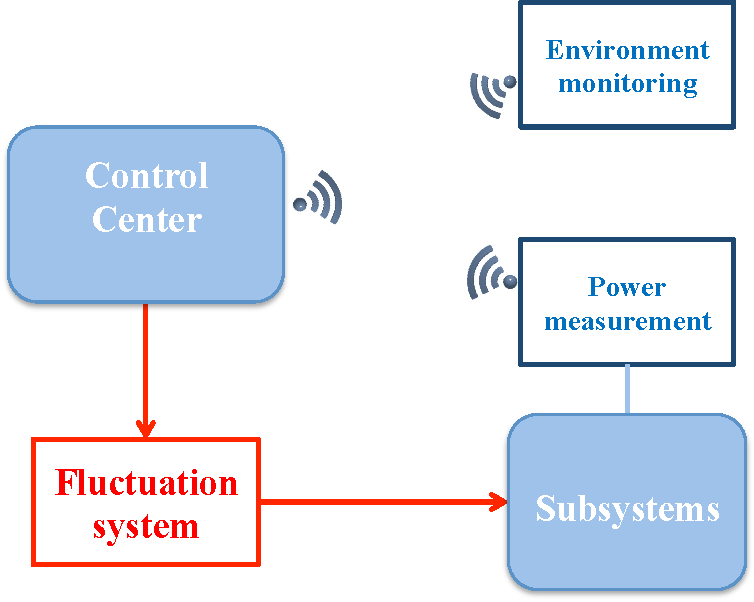
\includegraphics[width=0.6\textwidth]{./chapters/chapter1/images/SBA.pdf} 
\caption{Principle components of a SBA system.} 
\label{fig:I1} 
\end{figure}

The monitored environmental parameters can be occupancy, light intensity, temperature, moisture, sound, etc. Detecting and analyzing these information allows the system to automatically regulate the equipment to comfort the users, especially with the devices requiring time to start up such as HVAC system, and to regulate the power consumption. Except for occupancy, other types of environment can be easily monitored by the corresponding sensors such as light sensors, temperature sensors, humidity sensors, microphones, etc. Meanwhile, the occupancy detection is an interesting subject for many recent researches~\cite{Agarwal11ACM,Weng12DTC,Agarwal10BuildSys,Lu10ACM}. The occupancy can be detected directly by a Passive Infrared Sensor (PIR) or camera~\cite{Weng12DTC,Agarwal11ACM,Agarwal10BuildSys}, or indirectly by analyzing the events happening inside house or building, e.g. door state, variation on the total power signal~\cite{Chen13ACM}, abnormally increase of  the CO2 concentration~\cite{Wang01111999}.
For example, a couple of magnetic Reed Switch (RS) door sensor and PIR sensor can be used to detect the occupancy in offices or rooms~\cite{Agarwal11ACM,Weng12DTC}. Although PIR sensors are the most ubiquitous form for motion sensing, it is not enough for occupancy detection because people inside rooms/offices tend to maintain their posture when working in front of a computer, watching television or sleeping. To overcome this challenge, combining with an RS door sensor, which can determine if the door is open or closed, is more efficient. 
\begin{figure}
\centering
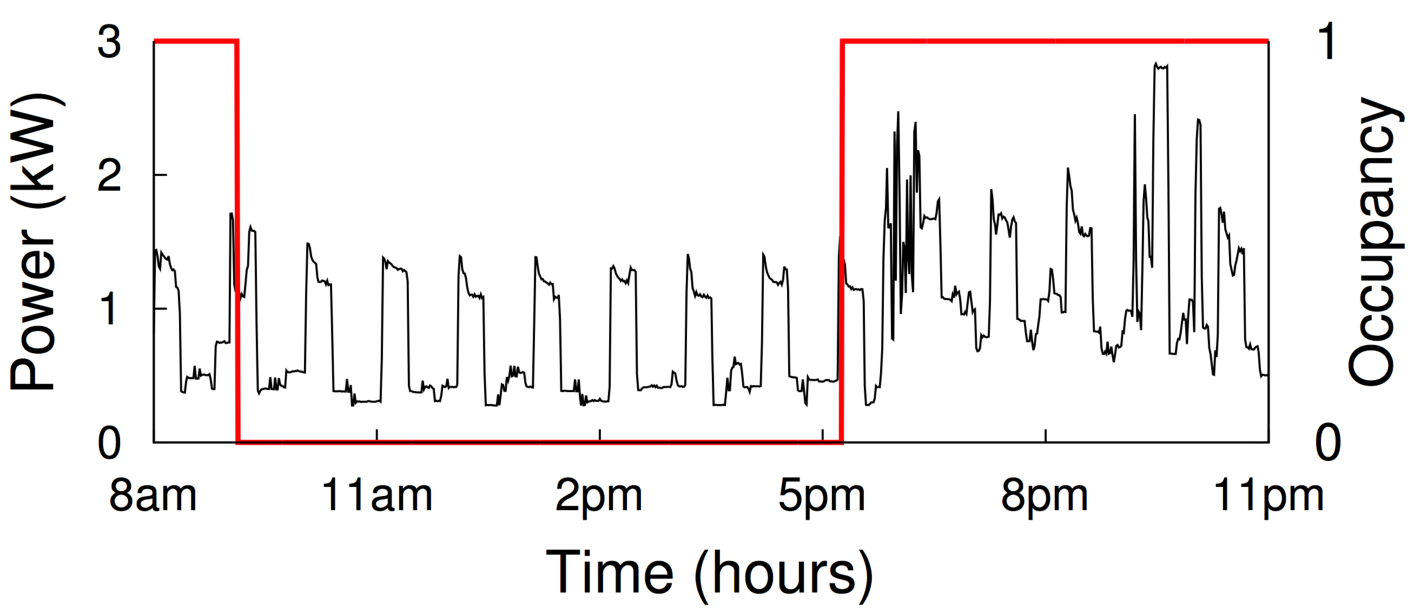
\includegraphics[width=0.7\textwidth]{./chapters/chapter1/images/nonintrusive_occupant_power.pdf} 
\caption{Variation on the power signal when the occupant turns on some devices~\cite{Chen13ACM}.} 
\label{fig:I2} 
\end{figure}
%---------------------------------
Another example of occupancy monitoring is to detect the large changes on the aggregate power signal and infer the occupancy~\cite{Chen13ACM}. As shown in~Figure~\ref{fig:I2}, the background load frequently appears and does not imply the occupancy. This load is derived from the presence of the devices driven by an automated controller such as fridge or HVAC system. When having the presence of the occupants, their physical interactions with loads such as switching on the lamp, turning on the television, etc., will imply changes on the power signal.
The large changes can be detected by comparing the average power, standard deviation or power range in a sliding window of signal with corresponding thresholds. Obviously, the accuracy of this monitoring system strongly depends on the survey of background load due to the variation of this parameter according to the time of day and year such as day or night, spring or winter.
Besides, the state transition of some types of devices can also provide the interaction of users~\cite{Ridi15}. For example, a washing machine has five states including off, wash, rinse, spin and maintenance wash, the user interaction can make the transition from the first to the second state.

In SBA, besides the environment monitoring, the power consumption of the equipment also needs to be measured and reported so that the control center can make a suitable fluctuation to adapt to the environmental variation.


\section{Thesis contributions}
%\subsection{Intrusive Load Monitoring}
Similar to the environment monitoring sensors, power measurement units also require a wireless protocol to communicate with the control center. Power metering can be implemented by two ways: intrusive and non-intrusive. In intrusive approach, the measurement is deployed at each individual equipment. In contrast, the Non-Intrusive Load Monitoring (NILM) \footnote{sometimes also referred as NIALM (Non-Intrusive Appliance Load Monitoring) or Electrical Load Disaggregation} can detect and estimate the power consumption of all devices on the monitored branch circuit with only one power meter installed on the main power entry~\cite{Hart92}. Intuitively, non-intrusive approach helps to reduce the deployment cost but requires a long period of observation to analyze the power characteristics of each device. 

As shown in Figure~\ref{fig:I3}, an Intrusive Load Monitoring (ILM) system can be implemented in a direct of indirect method. The direct one attaches a power meter to each device. Therefore, direct ILM obviously performs with high accuracy but has some disadvantages such as high cost and interruption on the power supply to install the meters. In contrast, the indirect method uses low-cost sensors to detect the measurable signals emitted by the device to estimate the power consumption. For example, a light sensor can detect the power state of a television and infer the corresponding consumed energy, an acoustic sensor can be applied to recognize the operation of the fridge compressor~\cite{Kim09Ubicomp}. 

\begin{figure}
\centering
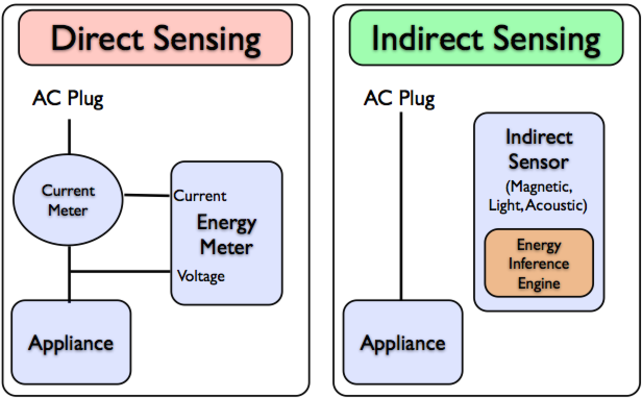
\includegraphics[width=0.8\textwidth]{./chapters/chapter1/images/direct_indirect_sensing.pdf} 
\caption{Direct and indirect power measurement \cite{Kim09Ubicomp}.} 
\label{fig:I3} 
\end{figure}
%---------------------------------




%\subsection{Non-Intrusive Load Monitoring}\label{nilm}

In contrast with intrusive approaches, the non-intrusive ones rely on only one power meter at the main power supply. An NILM algorithm tries to extract some specific features from the aggregate power signal to identify the corresponding devices.
Assuming there are $N$ devices connected to a unique power meter, each device $i\in \{1,\ldots, N\}$ can operate at one state $j$ of $m_i$ modes, which consumes a power of $w_{ij}$, $j \in \{1,\ldots,m_i\}$. Denote $s_{ij}(t)$ as the Boolean indicator of state $j$ of device $i$ at time $t$:
\begin{equation*}
s_{ij}(t)=\begin{cases}
1 \mbox{ if device $i$ operates at state $j$}\\
0 \mbox{ otherwise}.
\end{cases}
\end{equation*}
The aggregate power consumption can be represented as follows:
\begin{equation}\label{eqI6}
x(t)=\sum_{i=1}^{N}{\sum_{j=1}^{m_i}{s_{ij}(t)\times w_{ij} + e(t)}},
\end{equation}
where $e(t)$ is a noise or error term. From this model, the vector $\mathbf{s}$ containing all state indicators $s_{ij}$, $i=1,\ldots,N, j=1,\ldots,m_i$ of the devices from $1$ to $N$ can be determined by solving the following minimization problem:
\begin{equation}\label{eqI7}
\hat{\mathbf{s}}(t)=\argmin_{\mathbf{s}(t)}{\parallel x(t) - \sum_{i=1}^{N}{\sum_{j=1}^{m_i}{s_{ij}(t)\times w_{ij}}} \parallel_d},
\end{equation}
where $\parallel.\parallel_d$ denotes the $l_d$ distance. In the context of NILM, we can use some distance metrics such as $l_1$, $l_2$.
This problem is computationally intractable and impractical to be exactly solved by exhaustive techniques unless $N$ is small. Instead, heuristic algorithms might be considered. There are three principles for any NILM algorithm, including:
\begin{itemize}
\item Select and mathematically characterize the specific features or signatures.
\item Deploy the suitable hardware  to measure the desired signal.
\item Develop an algorithm to detect those features/signatures from the signal.
\end{itemize}
The characterization of features and signatures needs the knowledge on the operation states of the devices, which can be categorized into four types, as surveyed in \cite{Zoha12}, including:
\begin{itemize}
\item Type-I: devices with two states (ON/OFF) such as lamp, toaster, etc.
\item Type-II: finite state machines with a finite number of operation states, e.g. washing machine, stove, etc.
\item Type-III: continuously varying devices with variable power consumption such as power drill or dimmer lights.
\item Type-IV: devices that remain active throughout days or weeks and consume a constant level of power such as smoke detector, internet modem, etc.
\end{itemize}
The three first categories are proposed by \cite{Hart92} and shown in Figure~\ref{fig:I4}, while the last one is highlighted in \cite{Zeifman11TCE,Baranski03}. Besides, the selection of features/signatures also depends on the sampling frequency of meters and can be divided into two groups: low frequency  and high frequency.
Algorithms based on low-frequency signal focus on detecting the steady-state features such as average power, step-changes, etc., while high-frequency hardware allows us to identify the devices from the transient phase and harmonics.
\begin{figure}
\centering
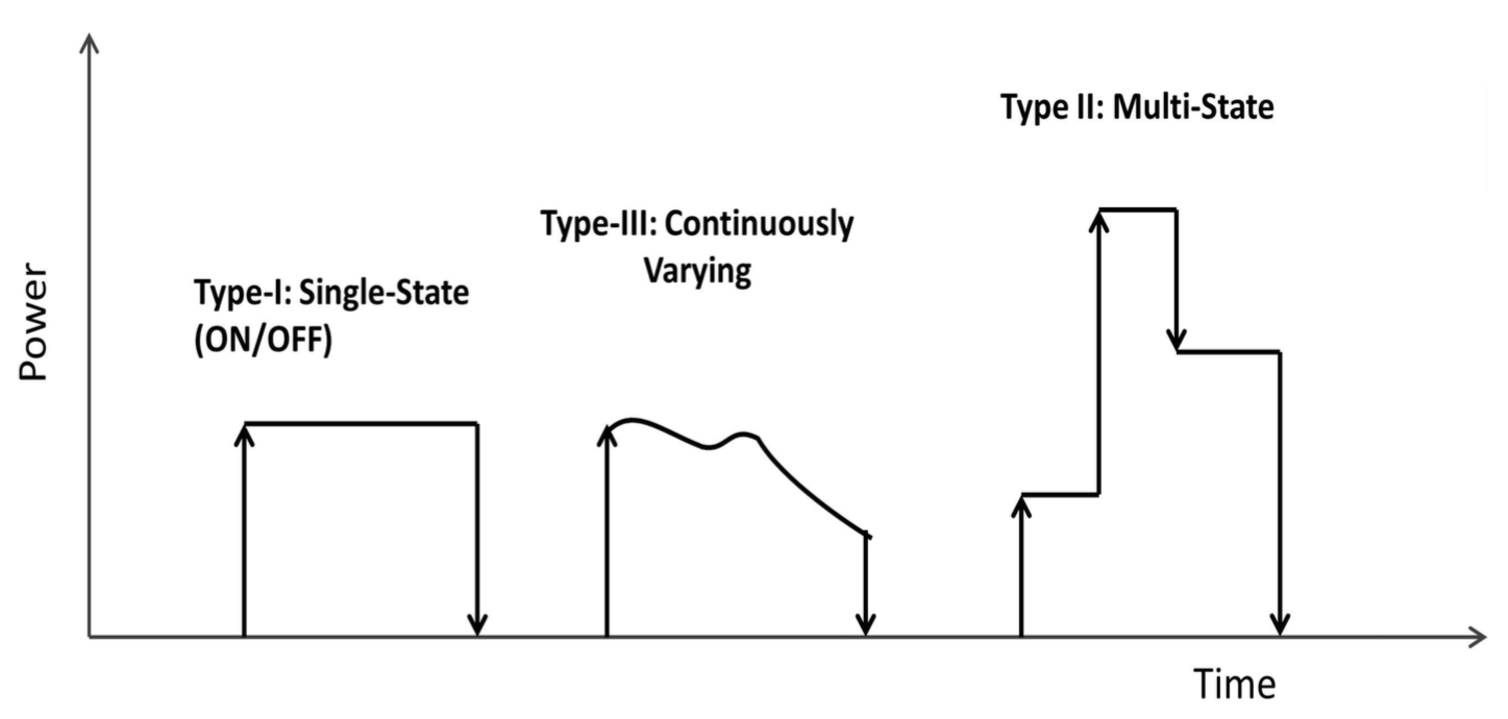
\includegraphics[width=0.8\textwidth]{./chapters/chapter1/images/load_categories.pdf} 
\caption{Different categories of load based on energy patterns \cite{Zoha12}.} 
\label{fig:I4} 
\end{figure}

%\subsection{Hybrid Load Monitoring}
A hybrid approach between intrusive and non-intrusive load monitoring, called Hybrid Load Monitoring (HLM), was proposed in recent years~\cite{TangW16,Berges10,Berges11,Guvensan13,Uddin12}. In this approach, a sensor network is deployed in homes to monitor the environmental parameters such as acoustic noise, light intensity, occupancy, etc., to detect the operation of some specific devices. The difference between the hybrid and intrusive approaches is that the sensors are only installed to monitor a part of all devices while the others are still identified by an NILM algorithm with aggregate power measurement. Therefore, HLM allows for a reduction of the cost of the intrusive approach and an increase of the detection accuracy of the non-intrusive one. In the context of this thesis, we will focus on hybrid methods in order to improve the performance of the existing NILM algorithms.


\section{Dissertation Organization}

\textbf{Chapter 2: State of the art}\\
This chapter reviews the techniques and approaches used in load monitoring, from intrusive to non-intrusive and from low frequency to high frequency sampling hardware. 
In intrusive approach, each device is attached to a set of sensors, which detect the environmental variation generated by the device and infer its power state. Although this approach shows a high accuracy, it is difficult to deploy in smart homes and buildings because of high cost and too much technical intervention on the infrastructure. 
Instead, by using only one power meter at the main entry of electricity, non-intrusive approach is more promising to study. In this approach, the electrical features of each device are characterized and an algorithm is developed to extract the features from the aggregate power load and therefore to identify the corresponding device.
The selection of electrical characteristics depends on the sampling frequency of hardware. Concretely, low frequency hardware is suitable for the stable loads with the features related to the average power demand, rising step-changes, falling step-changes, etc., while high frequency hardware is more efficient to identify the devices based on the transient signal and harmonics analysis. 
In recent years, a hybrid approach of intrusive and non-intrusive is studied, in which the sensors can be deployed to detect the state of several devices, while the rest is still recognized by a non-intrusive algorithm.

\textbf{Chapter 3: $l1$-norm minimization based algorithms for NILM}\\
In this chapter, the minimization problem in NILM is solved by directly using the brute force method to determine the state of each device. In this method, all possible combinations of operating devices are in turn applied to calculate the absolute error between their total power demand and the measured aggregate power. The set of devices giving the minimum error are identified as running. However, if there is more than one device having the same power demand, the detection is no more accurate. The main contribution of this chapter is to propose two solutions to overcome this challenge and to improve detection accuracy, including:
\begin{itemize}
\item Difference-based algorithm to compare the difference between the current state and the previous state of each device.
\item Probability-based algorithm to use the state transition probability to decide the operating devices.
\end{itemize}
An experiment is also implemented with a small set of devices installed our laboratory.

\textbf{Chapter 4: SmartSense: Sensor-Aided NILM}\\
The main contribution of this thesis, SmartSense system, is presented in this chapter. To improve performance of NILM algorithms, we propose to use the operating probability of each device as an external information. The probability can be estimated from a sensor network. Different from the intrusive approach, only a small subset of some devices are selected to be monitored by the sensors while the others are assumed to be equiprobable among the states. Although it could be perceived as similar to a hybrid approach, however, instead of identifying the state of devices from the sensor signals, we transform this state to a probability and an NILM algorithm can still be applied to all devices combined with this external information. Therefore, monitoring a set of devices can help to improve the detection of the others. The algorithms applied to SmartSense in this thesis include:
\begin{itemize}
\item Compositional Pareto-algebraic Heuristic.
\item Dynamic Programming.
\item Edge Detection.
\item Dynamic Time Warping.
\end{itemize}

These proposed algorithms are applied to both our own dataset as well as publicly available dataset. The evaluation of performance improvement is given in \textbf{Chapter 5: Experimental results}. Meanwhile, the conclusions and perspectives of this thesis will be presented in \textbf{Chapter 6: Conclusions and perspectives}.
 % Introduction//

% Chapter 1

\chapter{State-of-the-Art} % Write in your own chapter title
\label{SoA}
%\addtotoc{State of the Arts}
\lhead{\emph{State of the Art}} % Write in your own chapter title to set the page header

\section{Photonics interconnect}
\subsection{Transmitter}
\subsubsection{Lasers}
\subsubsection{Microring Resonators}
\subsubsection{Modulators}
\subsection{Receiver}
\subsubsection{Optical waveguides}
\subsubsection{Photodetectors}
A naive, intrusive and costly method to measure the power consumption of each device is to connect it to a  power meter. Apparently, this approach is practically unfeasible because of high cost and too much technical intervention on the power supply. Therefore, Kim et al.~\cite{Kim09Ubicomp} propose a so-called ViridiScope system to replace part of the power meters by indirect sensors to detect the environmental parameters around the monitored devices and deduce their power state. In this monitoring system, devices with stable loads can be monitored by indirect sensors such as light intensity sensors, acoustic sensors, etc., while devices with variable loads are attached to a magnetometer  or a direct power meter. A power meter is also installed at the main power line to measure the aggregate power consumption and an algorithm is developed to disaggregate this power to the corresponding devices.
An overview on the power estimation based on sensors and meters is presented in the following. 

\textbf{Magnetometer}: The magnetic field around device $i$ is sampled at 100~Hz and the signal $s_i(t)$ is formed from the standard deviation over one second sliding window. The corresponding power consumption correlated to this signal is estimated as:
\begin{equation}\label{eqA1}
x_i(t) = \alpha_i s_i(t)+\beta_i,
\end{equation}
where $\alpha_i$, $\beta_i$ are the calibration parameters. The magnetic field analysis method is also applied in \cite{Rowe2010}, but combined with electric field, as illustrated in Figure~\ref{fig:A1}. The electric field is generated from the difference of voltages, i.e. a strong electric field may be generated even when the device does not draw current, while magnetic field variations correspond to the changes in power consumption. Therefore, the electric field can be used to determine if the device is powered or not.

\begin{figure}
\centering
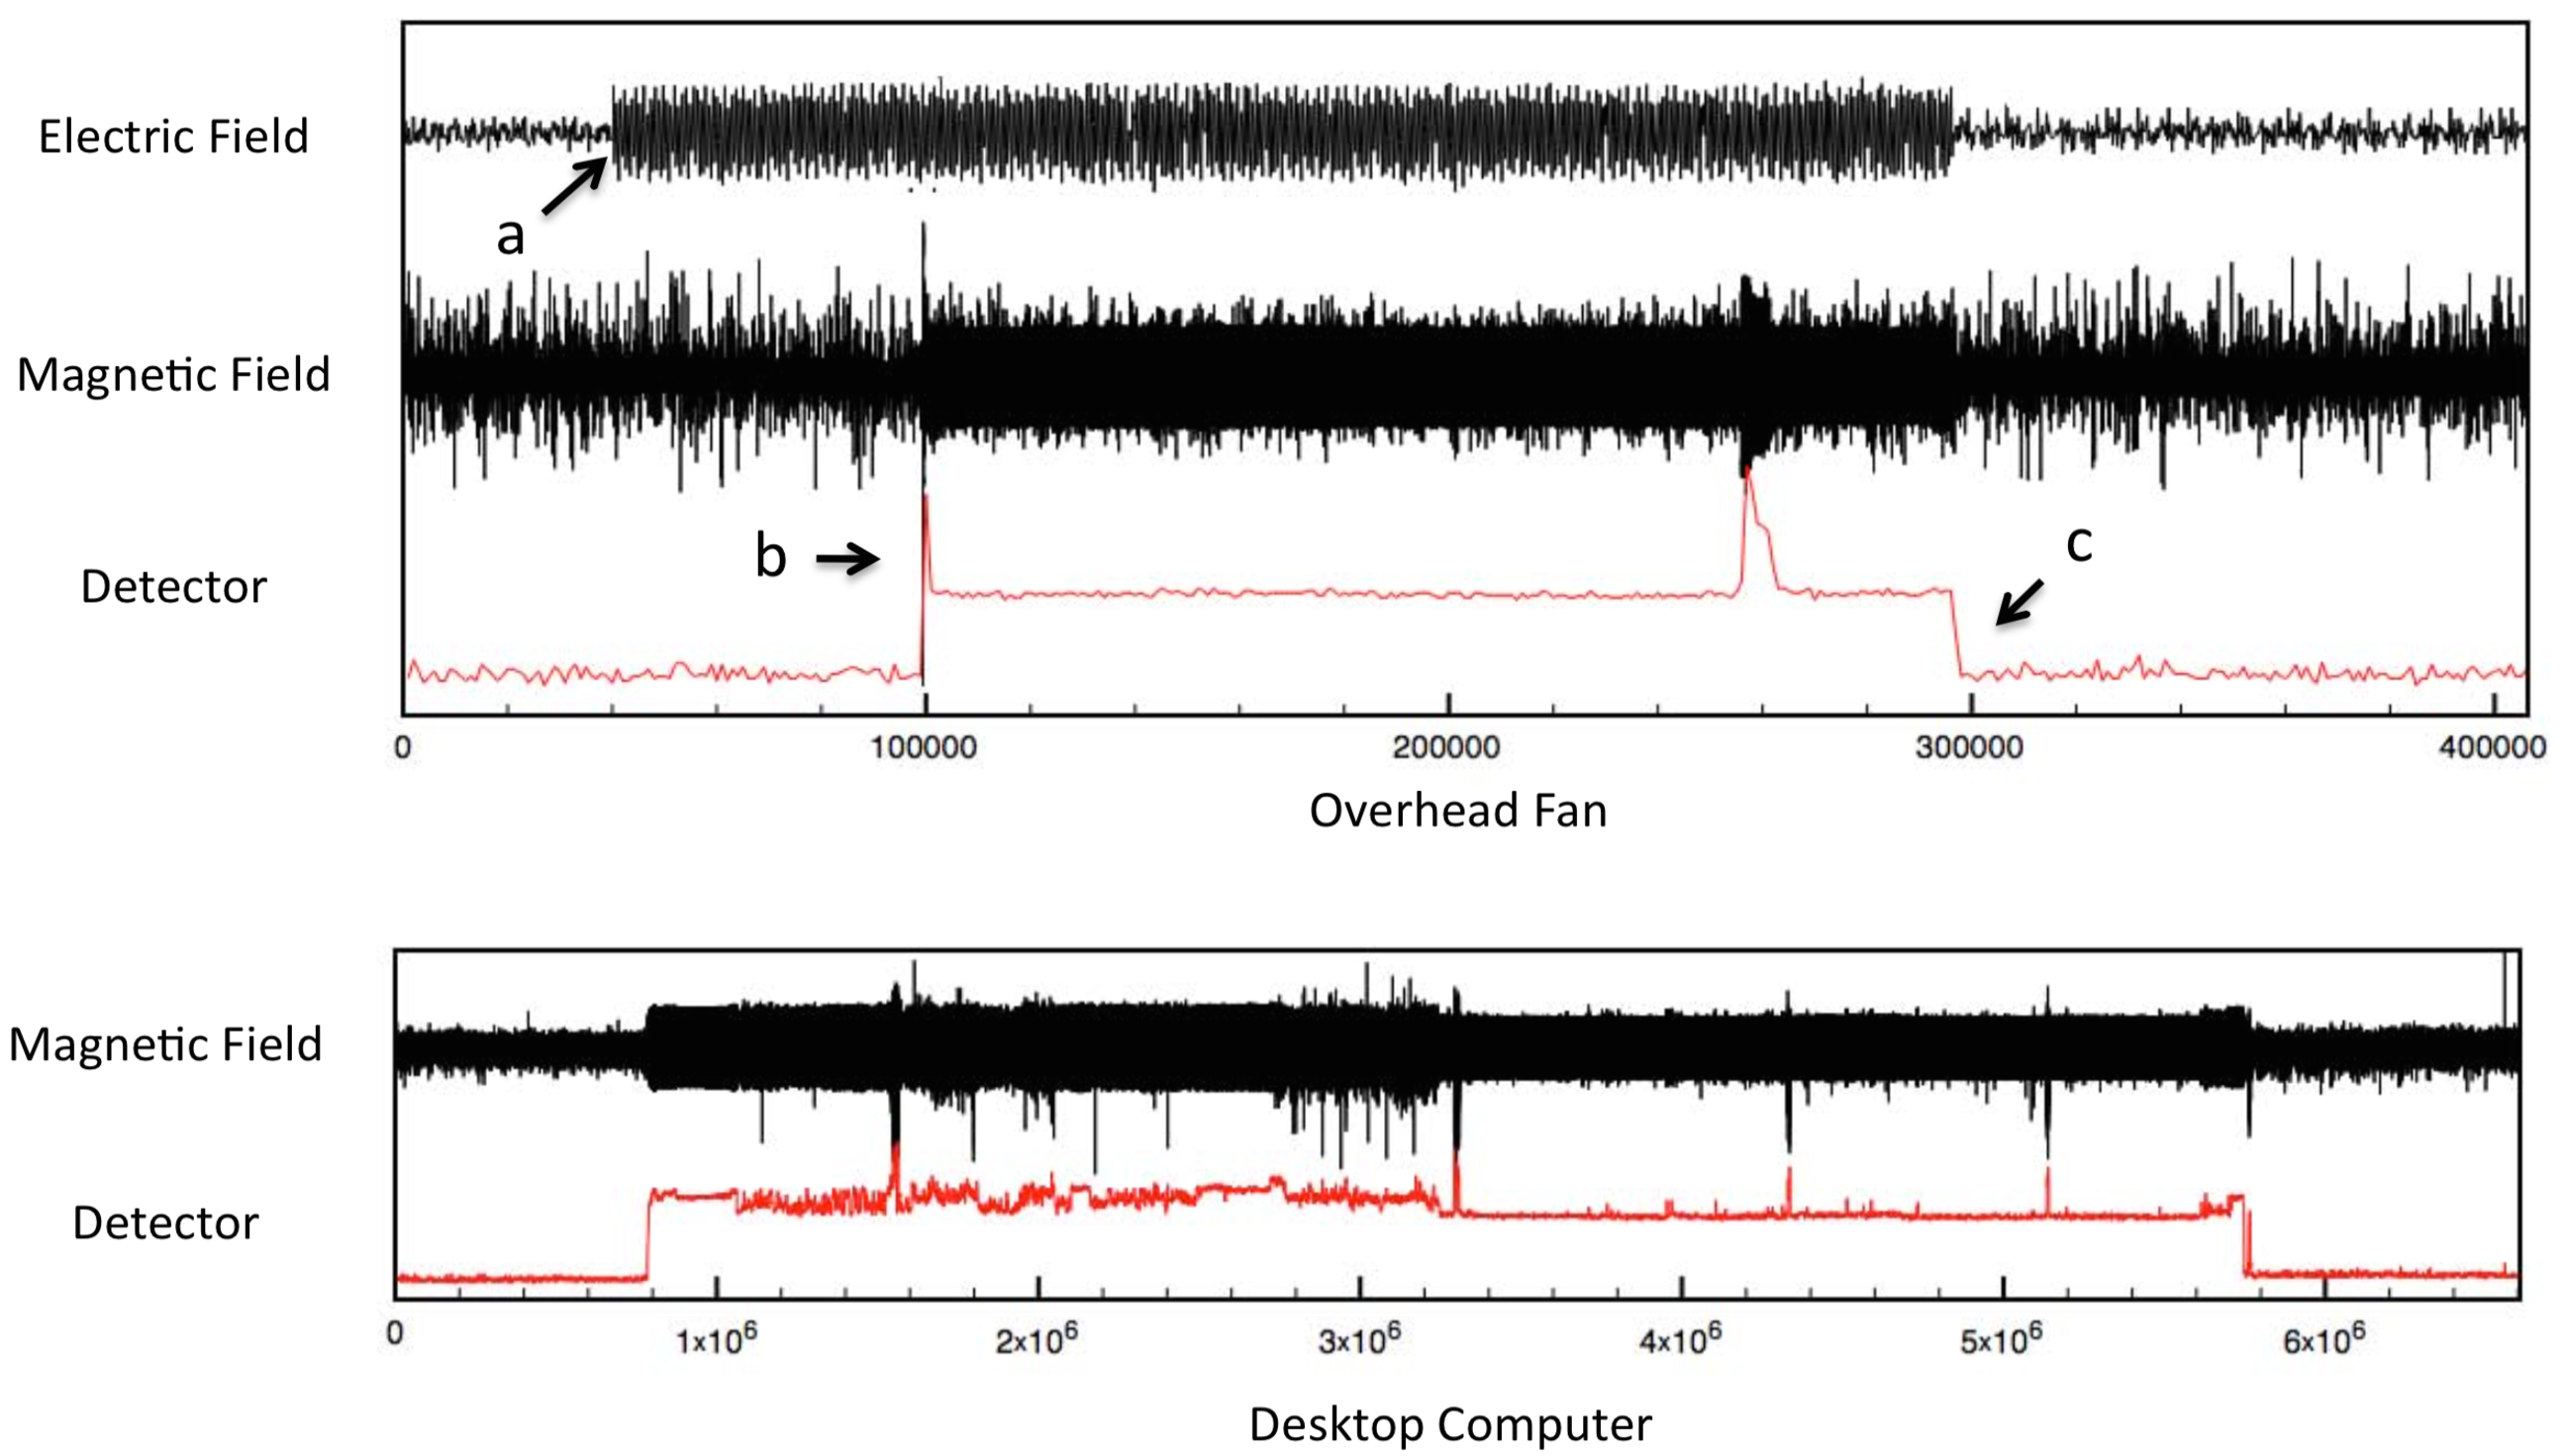
\includegraphics[width=0.8\textwidth]{./chapters/chapter2/images/EMFdetector.pdf} 
\caption{Electromagnetic field waveform. Top: Overhead fan is powered up at point (a), switched on at point (b) and switched off at point (c). Bottom: Variations in magnetic field near by a desktop computer~\cite{Rowe2010}.} 
\label{fig:A1} 
\end{figure}
%---------------------------------

\textbf{Environment monitoring sensors}: To estimate the power consumption of the devices with a limit number of power states, environment monitoring sensors, such as light or acoustic sensors, can be deployed. Denote $s_{ij}(t)$ a boolean indicator of the internal state $j$ of device $i$, the power consumption is estimated by:
\begin{equation}\label{eqA2}
x_i(t) = \sum_{j=1}^{M_i}{w_{ij}.s_{ij}(t)},
\end{equation}
where $M_i$ is the number of internal states of  device $i$ and $w_{ij}$  the average power demand of state $j$.

\textbf{Direct power meter}: There are still other devices monitored by a direct power meter and their power consumption is directly read from the meter. For device $i$,
\begin{equation}\label{eqA3}
x_i(t)=\tilde{x}_i(t),
\end{equation}
where $\tilde{x}_i(t)$ is the signal from the meter connected to device $i$.

\textbf{Uninstrumented devices}: Because of a large number of electrical loads in homes and buildings, some of them cannot be monitored by any meter or sensor. They are called uninstrumented devices. Their total power consumption can be considered as consumed by a unique device. Denote $w_i$ as the total power demand of these devices, their power consumption is estimated from the operating state as
\begin{equation}\label{eqA4}
x_i(t)=w_i s_i(t),
\end{equation}
where $s_i(t)$ indicates if the uninstrumented devices are present in the configuration or not.

Obviously, the total power consumption in home or building is the sum of the power consumption of all devices plus some noise and is defined as
\begin{equation}\label{eqAA5}
\begin{split}
 &x(t)=\sum_{i=1}^{N}{x_i(t)}+n(t)\\
\mbox{where}& \\
 &x_i(t)=\begin{cases}
\alpha_is_i(t)+\beta_i \mbox{: magnetometers}\\
\sum_{j=1}^{M_i}{w_{ij}s_{ij}(t)} \mbox{: light/acoustic sensors}\\
w_is_i(t) \mbox{: uninstrumented}\\
\tilde{x}_i(t) \mbox{: direct meter input}
\end{cases}
\end{split}
\end{equation}
where $N$ is the number of devices and $n(t)$ is a noise. To estimate the power demand of each device, i.e. $w_{ij}$ if monitored by sensors and $w_i$ if uninstrumented, as well as the calibration parameters $\alpha_i,\beta_i$, the following numerical optimization problem formulated from equations \eqref{eqA1}, \eqref{eqA2}, \eqref{eqA3}, \eqref{eqA4} needs to be solved:
\begin{equation}\label{eqA5}
 \min_\theta{\parallel x(t)-\sum_{i=1}^{N}{x_i(t)}\parallel},
\end{equation}
where $\theta$ is a vector containing all variables of power demand and calibration parameters, $\parallel . \parallel$ denotes the $l1$-norm or least absolute value regression solving for the median value. An example of power disaggregation in ViridiScope is represented in Figure~\ref{fig:A2}.

\begin{figure}
\centering
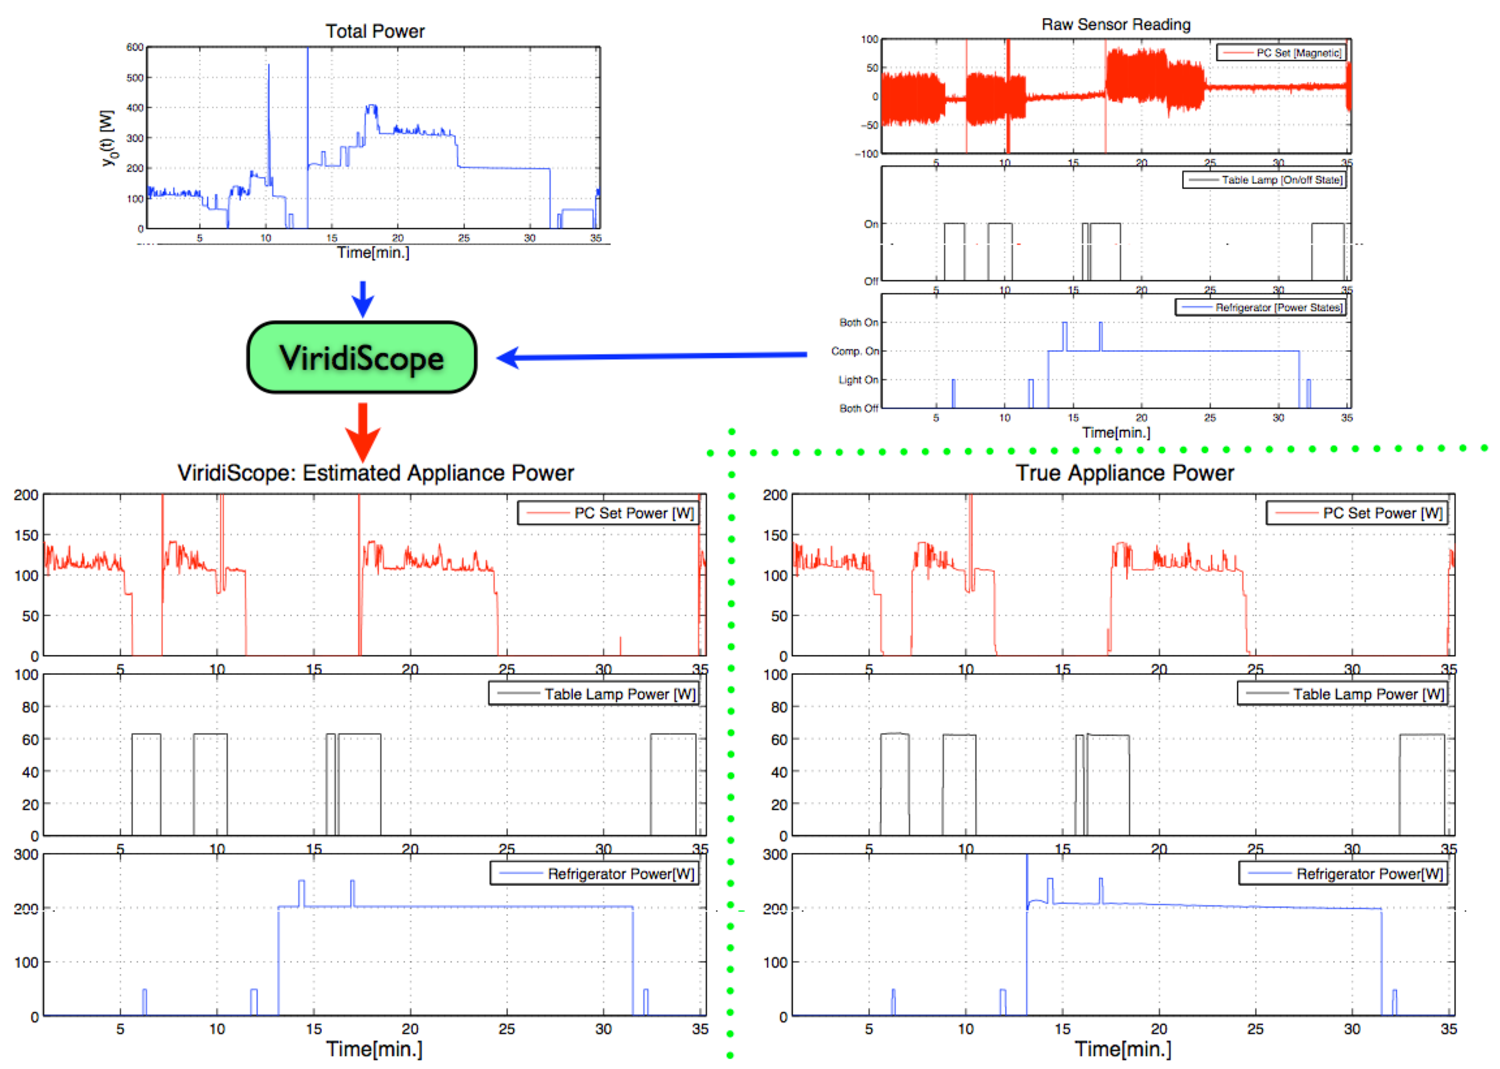
\includegraphics[width=1\textwidth]{./chapters/chapter2/images/ViridiScope_extract.pdf} 
\caption{The ViridiScope system considers the total power consumption, magnetic field signal and internal power state information to estimate the power consumption of each device by solving an $l1$-norm minimization problem~\cite{Kim09Ubicomp}.} 
\label{fig:A2} 
\end{figure}
%---------------------------------

Despite showing a high accuracy ($>90\%$) in the experiment \cite{Kim09Ubicomp}, ViridiScope still has some drawbacks. The first one is that the uninstrumented devices are assumed to consume a constant power, while this power can vary depending on the type of devices. The second limitation relates to the large amount of sensors necessary for deployment to reduce the number of uninstrumented devices and increase the accuracy of the system. 

Similar to ViridiScope, in~\cite{Jung2010,Jung2014}, the authors propose to use binary sensors to detect the on/off state of the energy consumers inside the buildings and then disaggregate the total power consumption to each one. The fundamental difference between this method and ViridiScope is to use the binary sensors providing the on/off state instead of raw data. All devices are assumed to consume a stable power level during their operation. That is the reason why the power consumption of the variable loads or multi-state devices cannot be accurately estimated. To increase the accuracy, the length of observation window used to estimate the power consumption of each device needs to be short enough. Besides, if the on/off sequences of more than two devices are synchronized, the power cannot be disaggregated. In this case, to reach a desired accuracy, some additional power meters are placed to the necessary electrical circuit branches, as illustrated in Figure~\ref{fig:A3}. In this example, because the on/off sequences of devices $x_2$ and $x_5$ are synchronized, their power is impossible to estimate if they are connected to the same power meter as in the left topology and topology 2. In contrast, in topology 1, these devices are connected to different circuit power meters, the disaggregation process can give a better performance. 

\begin{figure}
\centering
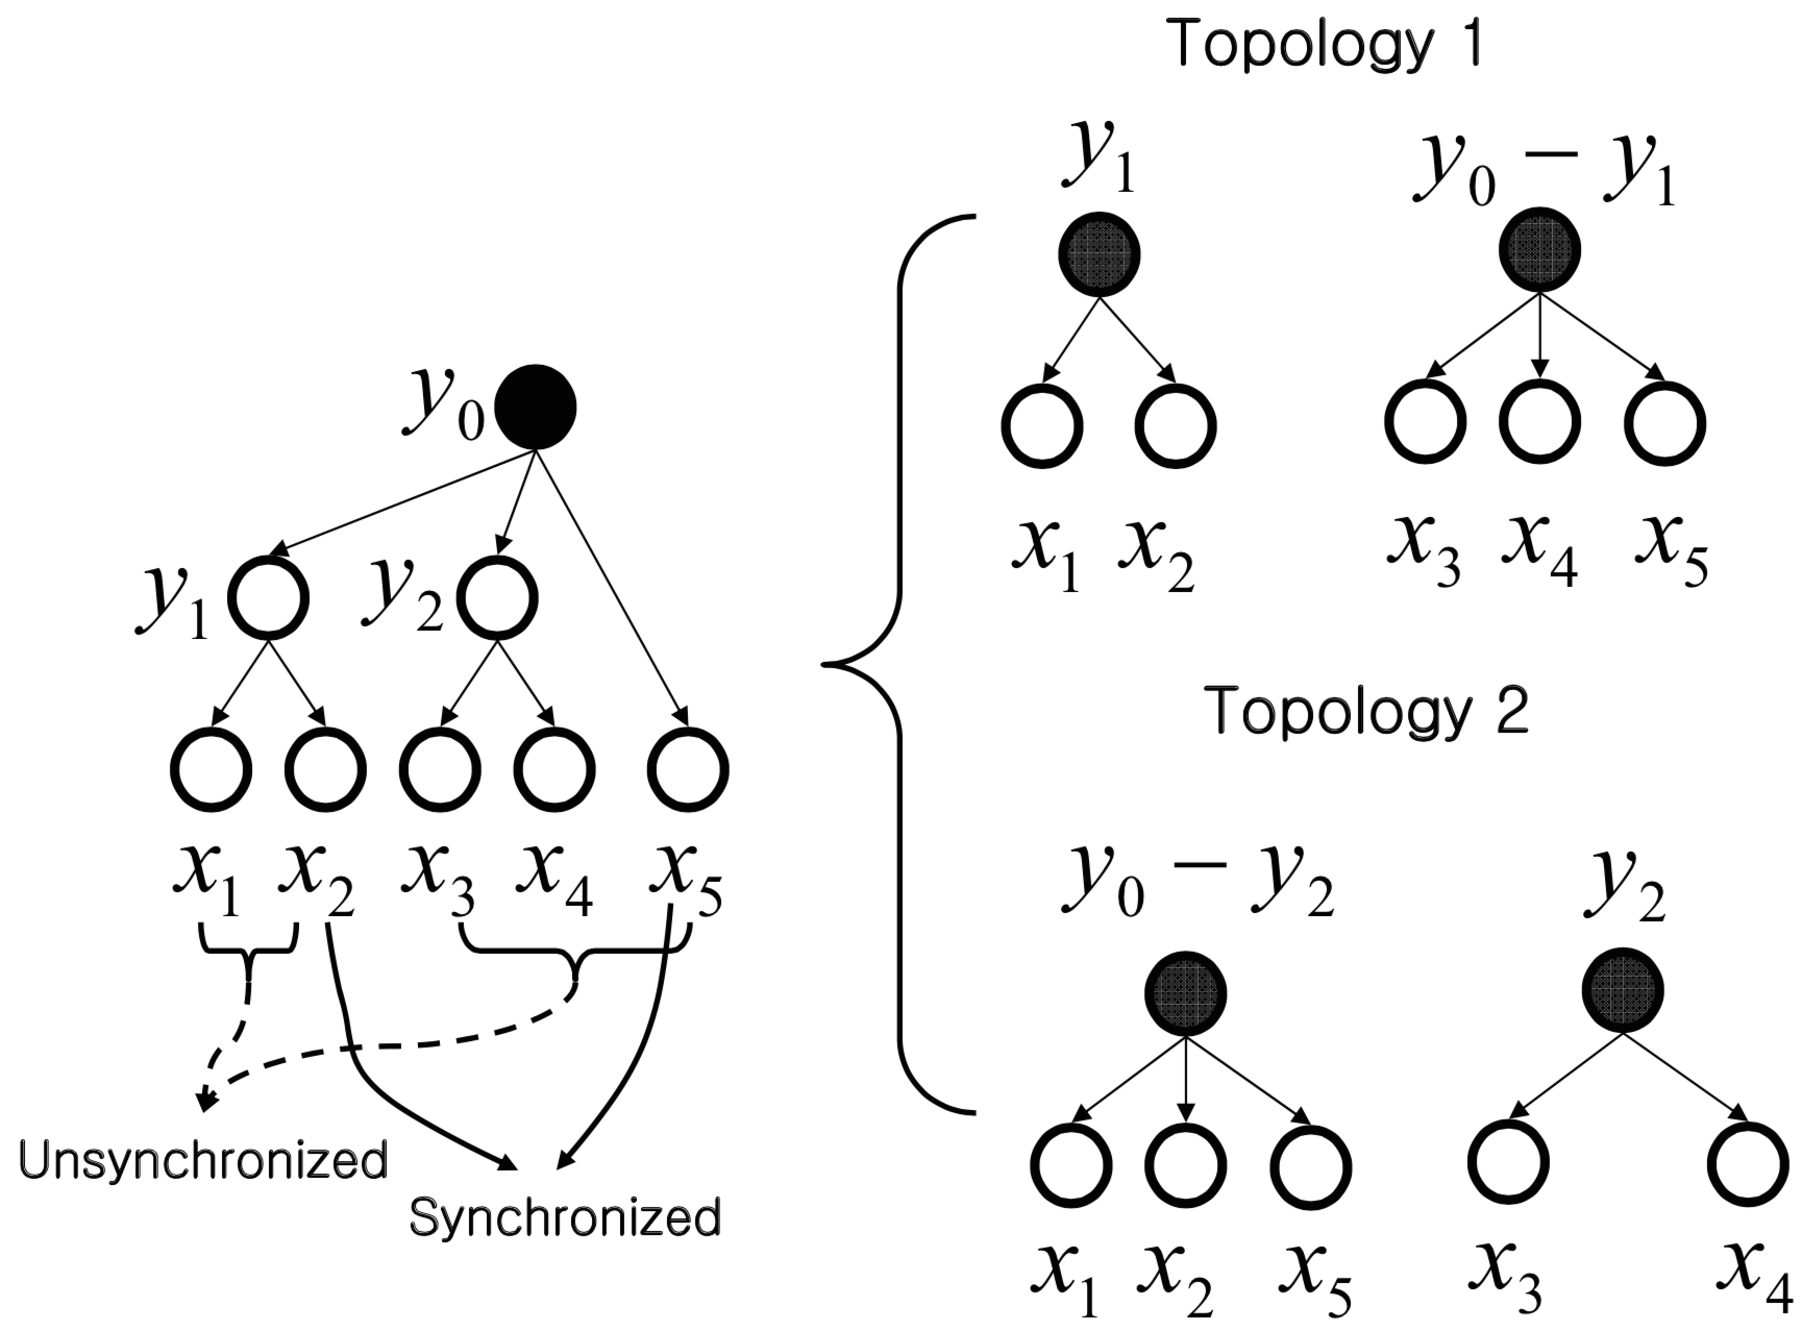
\includegraphics[width=.6\textwidth]{./chapters/chapter2/images/submeters.pdf} 
\caption{Power meter topology. The left topology uses only one power meter (dark node) at the main power supply while topology 1 and 2 use two additional power meters at the electrical circuit branches~\cite{Jung2010}.} 
\label{fig:A3} 
\end{figure}
%---------------------------------

A shortcoming of the research in \cite{Jung2010,Jung2014} is to ignore the presence of the \textit{ghost power} coming from the uninstrumented devices, that has strong effect on the performance when Beckel et al.~\cite{Beckel2012} apply this method to the Reference Energy Disaggregation Dataset (REDD)~\cite{Kolter11redd}. To overcome this problem, they assume to add  an always-on \textit{virtual ghost power consumer} to the set of monitored devices. They also assume that all devices are perfectly monitored by the binary sensors. By this way, the disaggregation can play a better performance, defined by the difference between the estimated power and real power consumption of each device.




\lhead{\emph{State of the Art}}
\section{CHAMELEON}\label{NILM}
Although direct power meters can be replaced by indirect sensors to reduce the deployment cost~\cite{Kim09Ubicomp,Jung2010,Jung2014}, a large amount of sensors as well as technical intervention is still required. To radically decrease the implementation cost, the presence of sensors needs to be eliminated or reduced as much as possible and the state of devices needs to be determined based on the aggregate power measured at the main power supply. This approach is called Non-Intrusive Load Monitoring or NILM and firstly proposed by G.~Hart~\cite{Hart92} in the early 1990s. In recent years, there are several industrial solutions hit to the market such as Wattseeker~\cite{Wattseeker}, Smart Analyzer~\cite{smartanalyzer}. In NILM, an algorithm is developed to detect some specific features to identify the operating devices. The features are selected depending on the sampling frequency of the meters and can be classified into two classes: low frequency and high frequency.

\subsection{Architecture}\label{macro}

In the low frequency approach, the promising features relate to the real and reactive power such as average power and step-changes when switching on/off or changing the power state of a device \cite{Hart92,Drenker99}. The step-change analysis method was firstly introduced by G.Hart \cite{Hart92}, in which the large changes on the power signal, as shown in Figure~\ref{fig:A4}, are detected by an edge detector. The edge detector firstly segments the power signal into steady periods, defined as a set of consecutive instants in which the power does not vary greater than a threshold. The samples in each period are then averaged and the difference between two consecutive steady periods is called step-size. Denote $x(t)$ as the measured power at time instant $t$, $x(t)$ is then expressed as
\begin{equation}
x(t) = \sum_{i=1}^N{x_i(t)+n(t)},
\end{equation}
where $N$ is the number of devices, $x_i(t)\geq 0 $ is the power consumption of device $i$ and $n(t)$ is a noise at instant $t$. A step-change is detected if $|x(t)-x(t-1)|\geq \gamma$, with threshold $\gamma$. An event is determined as started at time $t_s$ and ended at time $t_e$ if:
\begin{equation}
\left|(x(t_s)-x(t_s-1))+(x(t_e)-x(t_e-1))\right|\leq \alpha,
\end{equation}
where $\alpha$ is a practical estimated parameter.  A cluster analysis maps the detected step-changes to a two-dimensional space of real and reactive power. The rising edge (positive step-change) and falling edge (negative step-change) of an event (device activation) are then paired together and compared with the existing clusters from the training procedure to identify the corresponding load using maximum likelihood algorithm. Figure~\ref{fig:A6} shows the position of some devices on the P-Q plane.

\begin{figure}
\centering
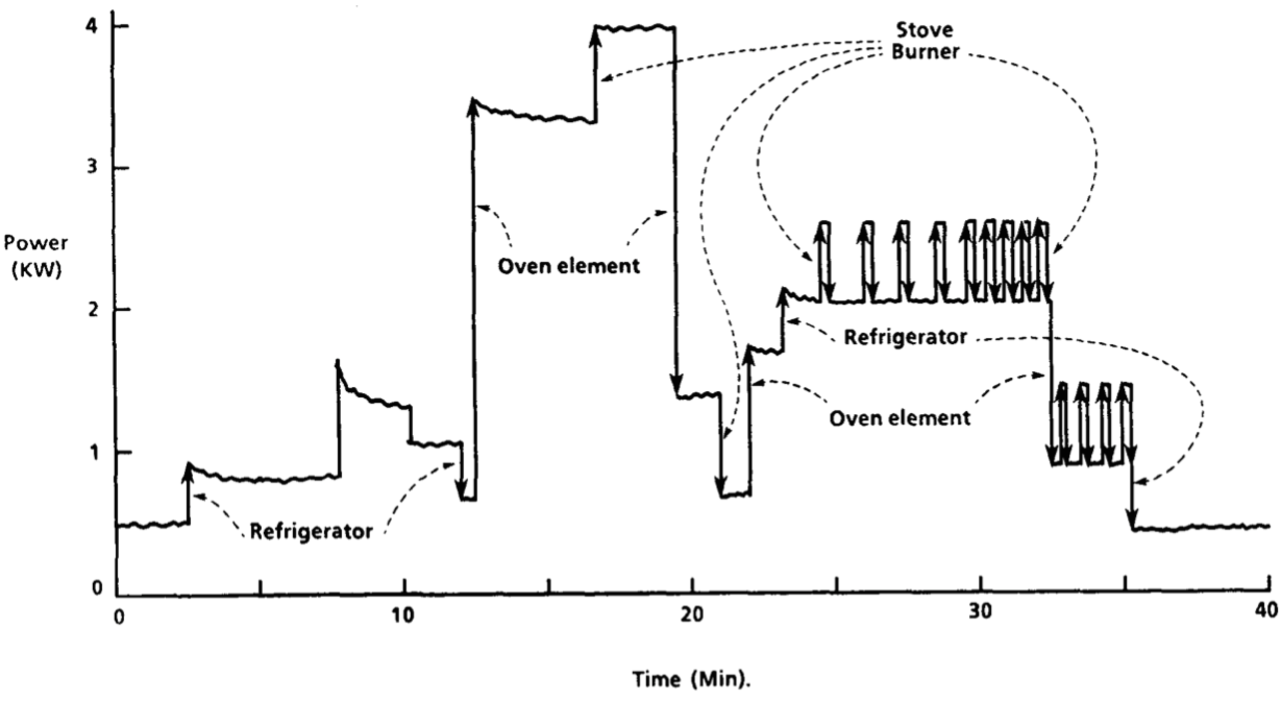
\includegraphics[width=0.8\textwidth]{./chapters/chapter2/images/step-change.pdf} 
\caption{Step-changes on the aggregate power signal~\cite{Hart92}.} 
\label{fig:A4} 
\end{figure}
%---------------------------------

The edge detector based method proposed in \cite{Hart92} is suitable to detect and identify the on/off events on the power signal. However, it cannot detect the variable loads such as computers, whose power consumption depends on the tasks. In addition, as illustrated in Figure~\ref{fig:A6}, the devices with overlapped clusters on the P-Q plane cannot be discriminated.

\begin{figure}
\centering
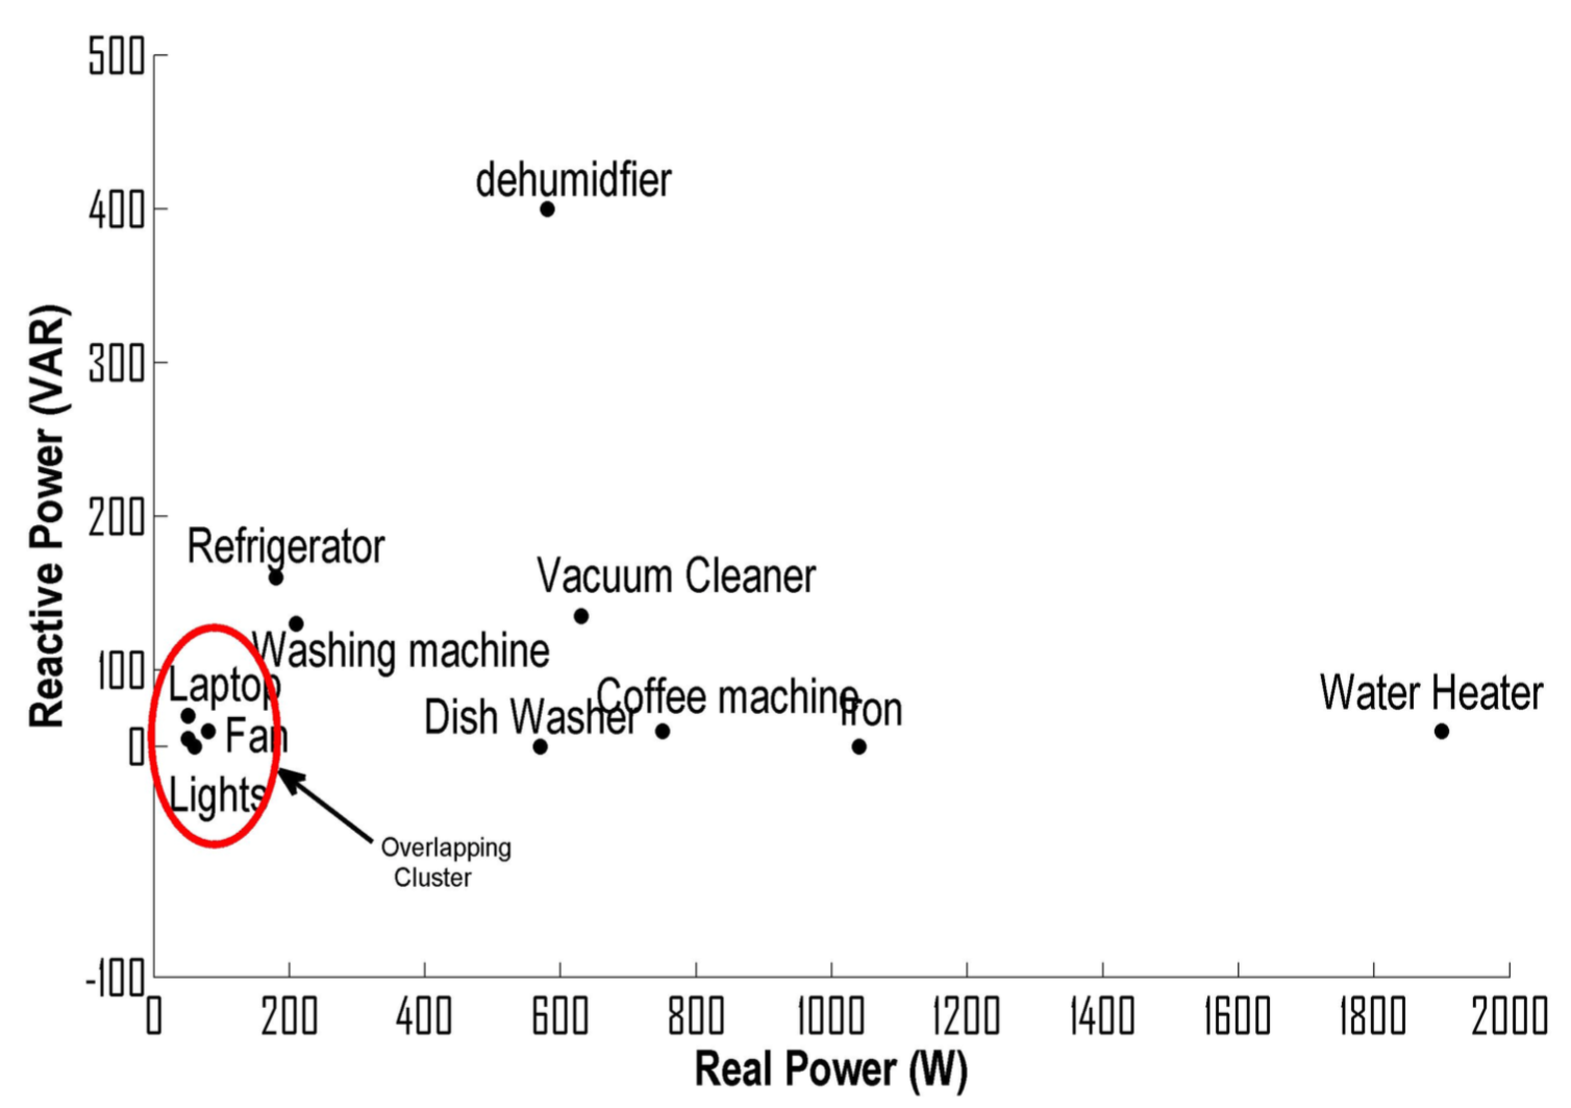
\includegraphics[width=0.8\textwidth]{./chapters/chapter2/images/overlap_PQplane.pdf} 
\caption{Load distribution in P-Q plane~\cite{Hazas11}.} 
\label{fig:A6} 
\end{figure}

To improve the performance of edge detection, some later researches are developed with some additional features. For example, in~\cite{Norford96,Marceau2000ECM}, a median filter is applied to remove the meaningless abrupt peaks in the raw signal, while in~\cite{Cole98IMTC}, edges and slopes, defined as the slow variations after an initial spike in the power signal when switching on a device, are simultaneously used as a feature to detect the devices necessary for a starting time before reaching the steady state such as heat pumps, dish washers, fridges, etc.

Similar to \cite{Hart92}, the authors of~\cite{Liao14} try to detect and pair the rising and falling edges of an event and construct a decision tree to identify the corresponding device. In the training phase, for each device, only edges with maximum and minimum height are saved instead of all possible ones. Thus, there are only $2N$ values in the library. 
The decision tree includes a\textit{ root}, several \textit{nodes} and \textit{leaves} relating to known or undefined devices. At each node, a split point value $V(node)$ calculated from the training data is used to decide the \textit{child} node, i.e. left or right. The splitting procedure iterates until any \textit{leaf} node is reached, i.e. the event is matched to a corresponding device.

Besides decision tree, another so-called Dynamic Time Warping (DTW) algorithm is also presented in~\cite{Liao14}. In this method, all active power values of an event from the rising edge to the falling edge are extracted and saved in a vector to create a pattern instead of only two edges. Because the lengths of the events are different, a pattern matching procedure via dynamic programming is proposed to apply. When a pattern is detected, the accumulated distance between it and all existing patterns in the library is calculated by Algorithm~\ref{algoA2}. The pattern giving the smallest distance is selected to identify the corresponding device. 

\begin{algorithm}[h]
\caption{Accumulated distance between two vectors with different lengths~\cite{Liao14}.}\label{algoA2}
\begin{algorithmic}[1]
\Function{DTW}{$p,q$}
	\State $n=\text{length}(p)$
	\State $m = \text{length}(q)$
	\State $D(0,0) = 0$, $D(i,0) = D(0,i)=\infty$
	\For {$i=1,\ldots,n$}
		\For {$j=1,\ldots,m$}
			\State $d(i,j)=|p(i)-q(j)|$
			\State $D(i,j) = d(i,j)+\min{\{D(i-1,j),D(i-1,j-1),D(i,j-1)\}}$
		\EndFor
		\State \textbf{end for}
	\EndFor
	\State \textbf{end for}
	\State Output $D(n,m)$
\EndFunction
\State \textbf{end function}
\end{algorithmic}
\end{algorithm}
The simulation results with REDD dataset~\cite{Liao14}, as shown in Table~\ref{TA1}, point out that the DTW algorithm outperforms the Hidden Markov Model (HMM) approach \footnote{presented later in this chapter} in terms of detection reliability as well as sensibility to the events. 
\begin{table}
\caption{Performance comparison between DTW and HMM approaches~\cite{Liao14}.}\label{TA1}
\begin{center}
\begin{tabular}{|c|c|c|c|c|}
\hline
 &\multicolumn{2}{|c|}{Reliability (\%)}  &  \multicolumn{2}{|c|}{Sensibility (\%)} \\ \hline
 House & DTW  & HMM & DTW  & HMM  \\ \hline
 House 1 & 85.01  & 79.29 & 79.72 & 62.72  \\ \hline 
 House 2 & 89.86  & 51.80 & 84.39  & 62.79  \\ \hline
 House 6 & 98.86  & 99.30 & 81.22  & 74.74  \\ \hline
\end{tabular}
\end{center}
\end{table}

The active power values can also be used to compute the load distribution~\cite{Chuang11}. Whenever an event is detected on the aggregate power signal, the corresponding load distribution will be calculated and compared with the library to identify the device. To get the load distribution when two or more devices operate at the same time, the convolution is applied to the distribution of the corresponding devices.
Meanwhile, the authors of \cite{Batra2013} apply the edge detector to each phase of electric power supply. This division helps to reduce the state space from $K^N$ down to $K^{N_p}$ if each device has $K$ states and each phase supplies the power for $N_p$ devices. Obviously, this method is efficient when applied in large buildings with more than one phase of electric power.

In another research, to identify large loads such as water heaters, the authors of~\cite{Farinaccio99EB} propose a so-called \textit{top-bottom rule-based} algorithm comprised of many decision rules applied to each detected pattern such as step-change, average power, total power, number of data points, etc. After comparing each component with the library, a final score is calculated to make a final decision about the operation of the corresponding device. Each type of devices is recognized by a different set of rules, which implies that this method need an excessive training and makes it difficult to be widely implemented.

Instead of detecting the events on the aggregate power signal, the raw power data can also be directly used in sparse coding~\cite{Kolter10,Pathak15}. In this method, the training data of each device is contained in matrix $\mathbf{W}_i\in \mathbb{R}^{T\times m}$ in which each column corresponds to the data of one week. The aggregate power consumption is then $\mathbf{W}=\sum_{i=1}^N{\mathbf{W}_i}$. Applying the sparse coding, the following approximation is considered: 
\begin{equation}
\mathbf{W}_i=\mathbf{B}_i\times \mathbf{A}_i, 
\end{equation}
where $\mathbf{B}_i\in \mathbb{R}^{T\times n}$ contains $n$ basis functions or \textit{dictionary}, and $\mathbf{A}_i\in \mathbb{R}^{n\times m}$ contains the \textit{activations} of basis functions. In the training period, the values of $\mathbf{B}_i$ and $\mathbf{A}_i$ are estimated by the following minimization:
\begin{equation}
\smash{\displaystyle\min_{\mathbf{A}_i\geq 0,\mathbf{B}_i\geq 0}{\frac{1}{2}\parallel \mathbf{W}_i-\mathbf{B}_i\times \mathbf{A}_i\parallel_F^2 + \lambda\sum_{p,q}{(\mathbf{A}_i)_{pq}}}} \mbox{ subject to } \parallel b_i^{(j)} \parallel_2 \leq 1, j=1,\ldots,n,
\end{equation}
where $\parallel \mathbf{Y}\parallel_F \equiv (\sum_{p,q}{\mathbf{Y}_{pq}})^{1/2}$ denotes the Frobenius norm, and $\parallel y \parallel_2 \equiv (\sum_{p}{y_p^2})^{1/2}$ is the $l_2$-norm.
To disaggregate a new set of data $\mathbf{X}\in \mathbb{R}^{T\times m'}$, the value of $\mathbf{A}_i$ is recalculated as
\begin{equation}
\begin{split}
\hat{\mathbf{A}}_{1:N}=&\argmin_{\mathbf{A}_{1:N}\geq 0}{\parallel \mathbf{X}-\left[ \mathbf{B}_1\cdots \mathbf{B}_N\right] \left[\begin{array}{c}\mathbf{A}_1\\ \vdots \\ \mathbf{A}_N \end{array}\right]  \parallel_F^2 + \lambda \sum_{i,p,q}{(\mathbf{A}_i)_{pq}}}\\
&\equiv \argmin_{\mathbf{A}_{1:N}\geq 0}{F(\mathbf{X},\mathbf{B}_{1:N},\mathbf{A}_{1:N})}.
\end{split}
\end{equation}
Finally, the power is disaggregated to each device by
\begin{equation}
\hat{\mathbf{X}}_i=\mathbf{B}_i\times \hat{\mathbf{A}}_i.
\end{equation}
Obviously, the sparse coding based disaggregation algorithm needs an excessive amount of training data. Additionally, this method is only used in off-line mode and not suitable for the real-time detection.


To recognize the large loads as in \cite{Farinaccio99EB}, Prudenzi~\cite{Prudenzi02} applies Artificial Neural Networks (ANN) to determine the time of use of three different loads from two groups including water heater (group H) and washing machine/dish washer (group W), as illustrated in Figure~\ref{fig:A10}. In the preprocessing stage, the daily data is sampled every 15 minutes and segmented into six 8-hour patterns with 4-hour overlapped interval. Then, to classify these patterns into two clusters with and without power activation (cluster P and cluster A, respectively), three parameters including maximum power, average power and maximum power change in each pattern are applied to a Self-Organizing Map (SOM). The patterns in cluster P are then sent to the identification stage comprising two supervised Back-Propagation neural Networks (BPN) with 32 inputs, 24 hidden neurons and 32 outputs. The first net (BPN1) tries to detect the instants with energy usage in each pattern and fills in a $6\times 32$-cell output table. After that, the output is filtered by multiplying by the output of the preprocessing stage and sent to the second net (BPN2), where the patterns of group H will be discriminated from group W by applying the moving average operation. The output of this net will only contain the power usage indicators of the water heater. Combining the outputs of two neuron nets, the time of use of both groups will be determined in the post-processing stage. Although this research only considered two groups of devices, it contributes a new promising approach for pattern identification by applying ANN.

\begin{figure}
\centering
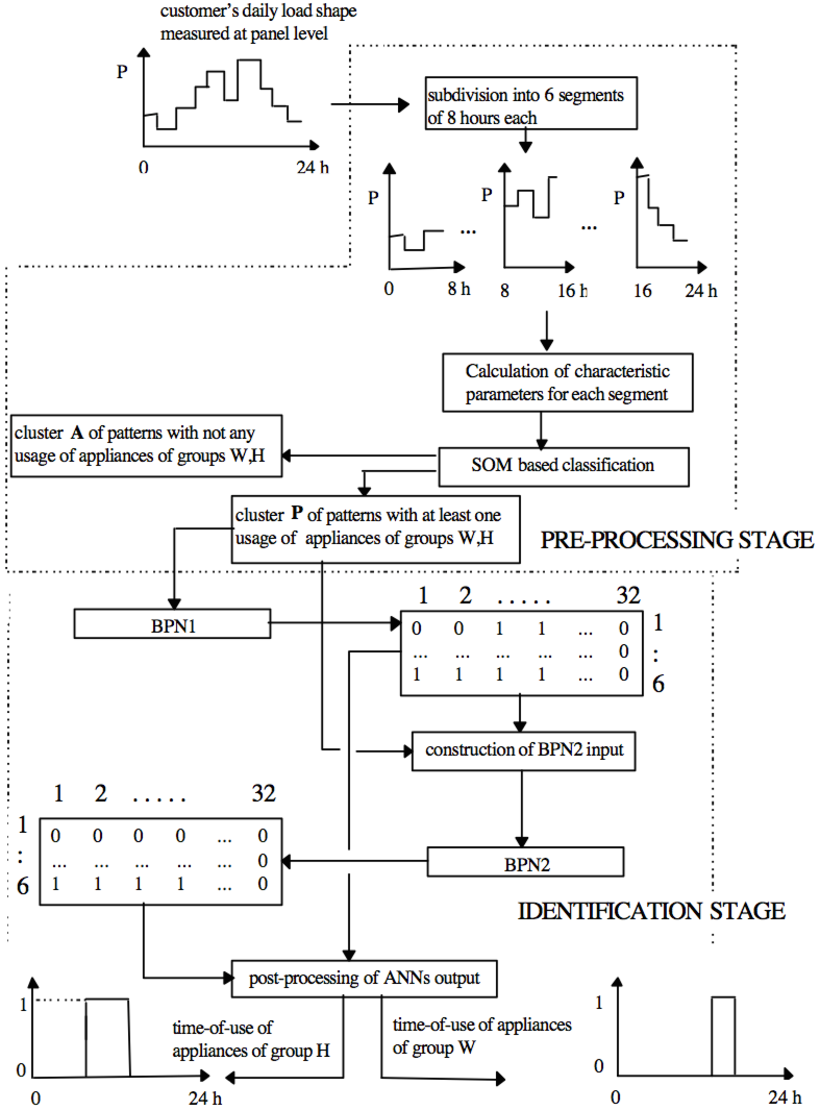
\includegraphics[width=0.6\textwidth]{./chapters/chapter2/images/3-stage_ANN.pdf} 
\caption{ANN to identify the water heater (group H) and washing machine/dish washer (group W)~\cite{Prudenzi02}.} 
\label{fig:A10} 
\end{figure}

Similarly, an ANN architecture is also applied in a system called real-time RECognition of electrical Appliances and Profiling (RECAP)~\cite{Ruzzelli10,Najmeddine08,Figueiredo11}, where the current and voltage waveforms are analyzed to extract the peak and Root Mean Square (RMS) values of both current and voltage, phase difference and power factor to define a profile of device. Besides, two other factors including signature length and sampling frequency are also captured to standardize the signatures from dissimilar types of energy meters. Although the RECAP system can profile and recognize the devices under a single framework and show a good performance when identifying the kitchen devices, it is not suitable for the multi-state devices.


% Add: Neural NILM

In another research, deep neural networks are constructed to disaggregate the domestic energy \cite{KellyK15} and applied to the UK Domestic Appliance-Level Electricity (UK-DALE) dataset \cite{UK-DALE}. The input of the network is a window of aggregate data with length determined by the maximum operating duration of the target device, while the output contains the information to reconstruct its power consumption. Before to be fed to the network, the input sequence in each data window is normalized by subtracting by the mean of sequence and by dividing by the standard deviation. The device activations used as the targets in training the networks are extracted based on some arguments such as maximum power, on-power threshold, minimum on-duration, minimum off-duration~\cite{Batra14}. The authors of \cite{KellyK15} propose three deep learning architectures to reconstruct the power consumption of target devices. The first one is a Recurrent Neural Network (RNN), which allows the output from each neuron in a layer at time step $t$ to be fed via weighted connections to all neurons of that layer at time step $(t+1)$. This makes RNNs suitable for the sequential data. To enhance the performance of RNNs in term of memory, the Long Short-Term Memory (LSTM) architecture \cite{Hochreiter97}, using the memory cells with a gated input, gated output and gated feedback loop, is applied. Besides, a bidirectional RNN, which is composed of two parallel RNNs, one for the input sequence forwards and one for the input sequence backwards, is also applied. The concrete architecture with type of each layer is as follows: Input $\rightarrow$ CONVolutional layer (CONV) $\rightarrow$ Bidirectional RNN layer (BiRNN) $\rightarrow$ BiRNN $\rightarrow$ Fully Connected layer (FC) $\rightarrow$ FC (Output). Examples of neural networks using CONV, BiRNN and FC are given in Figure~\ref{fig:AA3}.


The second deep learning architecture is Denoising Autoencoder (DAE) \cite{Vincent08}. The role of this architecture is to recover the power consumption of the target devices from the background noise. To do that, the DAEs at first try to encode the input to a compact vector with a coding layer and then decode it to reconstruct the input. The proposed architecture of DAEs includes six layers, in which the first convolutional layer can be considered as an encoder and the last one is a decoder, as follows: Input $\rightarrow$ CONV $\rightarrow$ FC $\rightarrow$ FC $\rightarrow$ FC $\rightarrow$ CONV (Output).


Meanwhile, in the last architecture, the power activation in each data window can be reconstructed by detecting the  start time, end time and average power consumption. In other words, they want to draw a rectangle around each activation in which the left side is the start time, right side is the end time and the height is the average power. Therefore, the output layer of this network includes three neurons and the output data are encoded to be in the range $[0,1]$. The exact architecture consists of eight layers: Input $\rightarrow$ CONV $\rightarrow$ CONV $\rightarrow$ FC $\rightarrow$ FC $\rightarrow$ FC $\rightarrow$ FC $\rightarrow$ FC (Output).
\begin{figure}[htb]
\begin{minipage}[h]{1\linewidth}
\centering
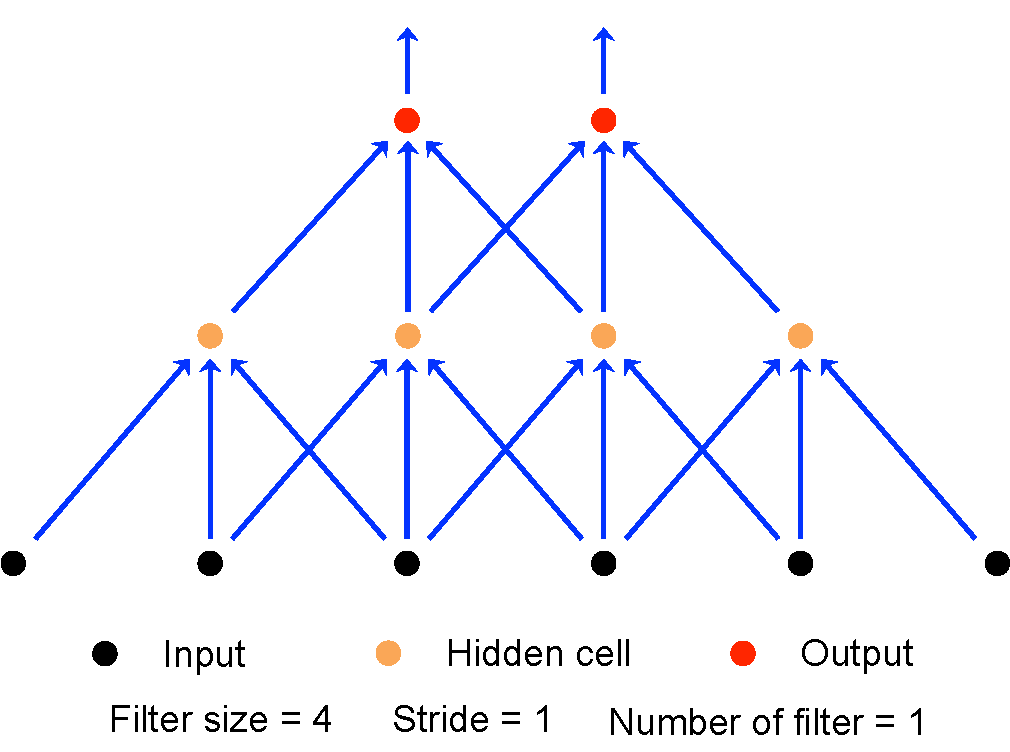
\includegraphics[width=0.48\textwidth]{./chapters/chapter2/images/ConvANN.pdf}
%  \vspace{1.5cm}
\centerline{(a) Convolutional neural network}\medskip
\end{minipage}
\hfill
\begin{minipage}[h]{1\linewidth}
\centering
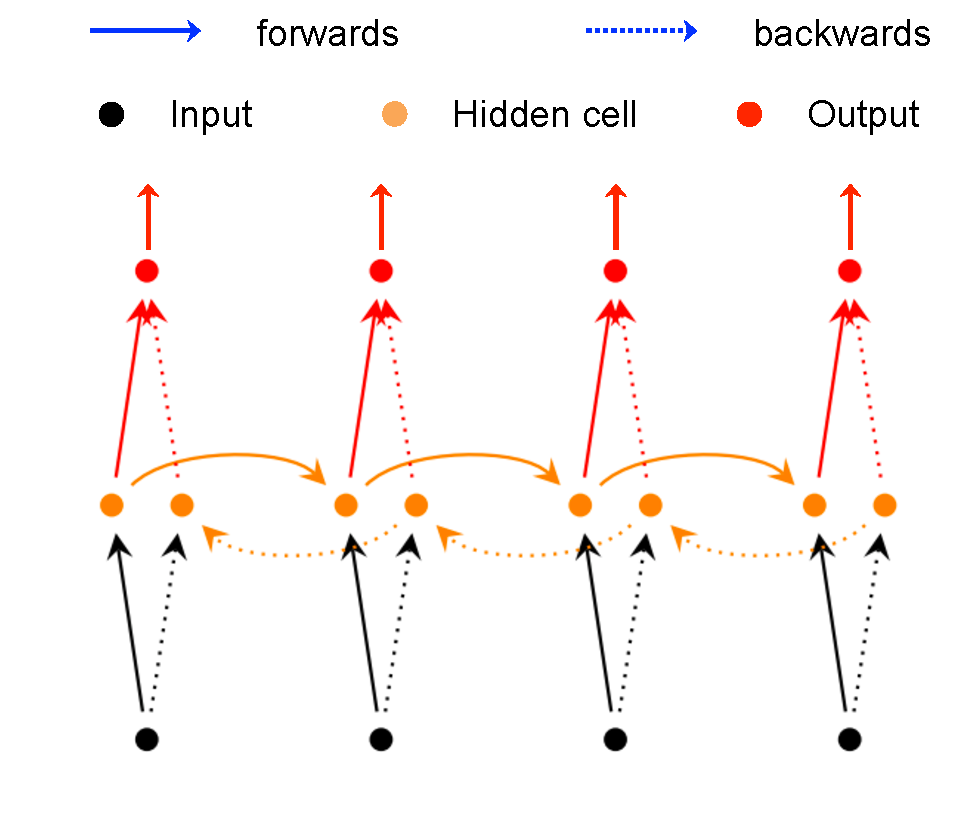
\includegraphics[width=0.48\textwidth]{./chapters/chapter2/images/BiRNN.pdf}
%  \vspace{1.5cm}
\centerline{(b) Bidirectional RNN}\medskip
\end{minipage}
\hfill
\begin{minipage}[h]{1\linewidth}
\centering
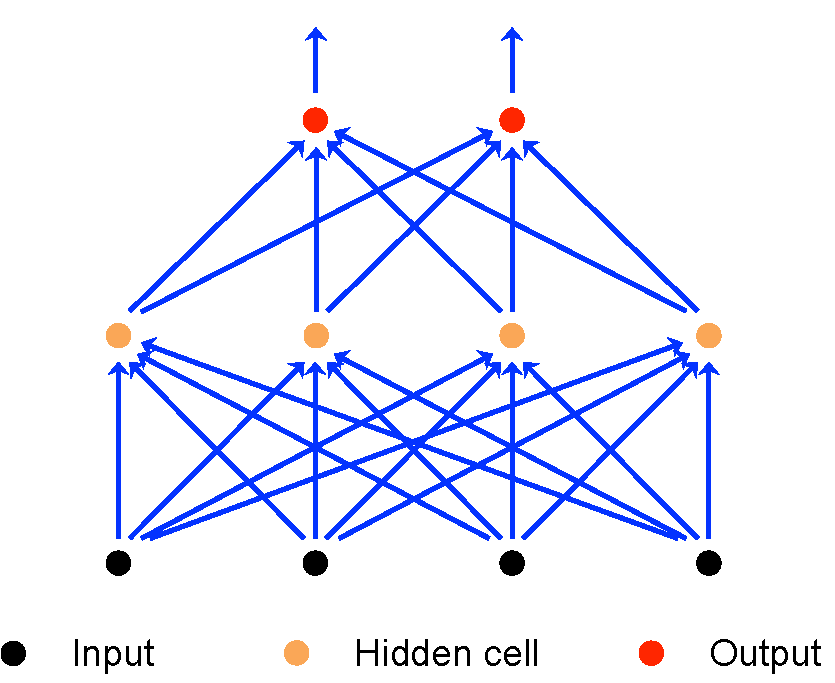
\includegraphics[width=0.48\textwidth]{./chapters/chapter2/images/fullyConn.pdf}
%  \vspace{1.5}
\centerline{(c) Fully connected neural network}\medskip
\end{minipage}
\caption{Examples of convolutional neural network, bidirectional RNN and fully connected neural network.}
\label{fig:AA3}
%
\end{figure}

Figure~\ref{fig:AA4} illustrates the outputs produced by three deep neural networks in~\cite{KellyK15}. Apparently, the DAE architecture performs a good estimation for the varying power consumers such as washing machine, while the third architecture (Rectangles) is suitable for the stable loads such as kettle, fridge. In addition, the RNN using LSTM architecture gives a worse estimation than DAE but better than Rectangles with variable loads.

\begin{figure}
\centering
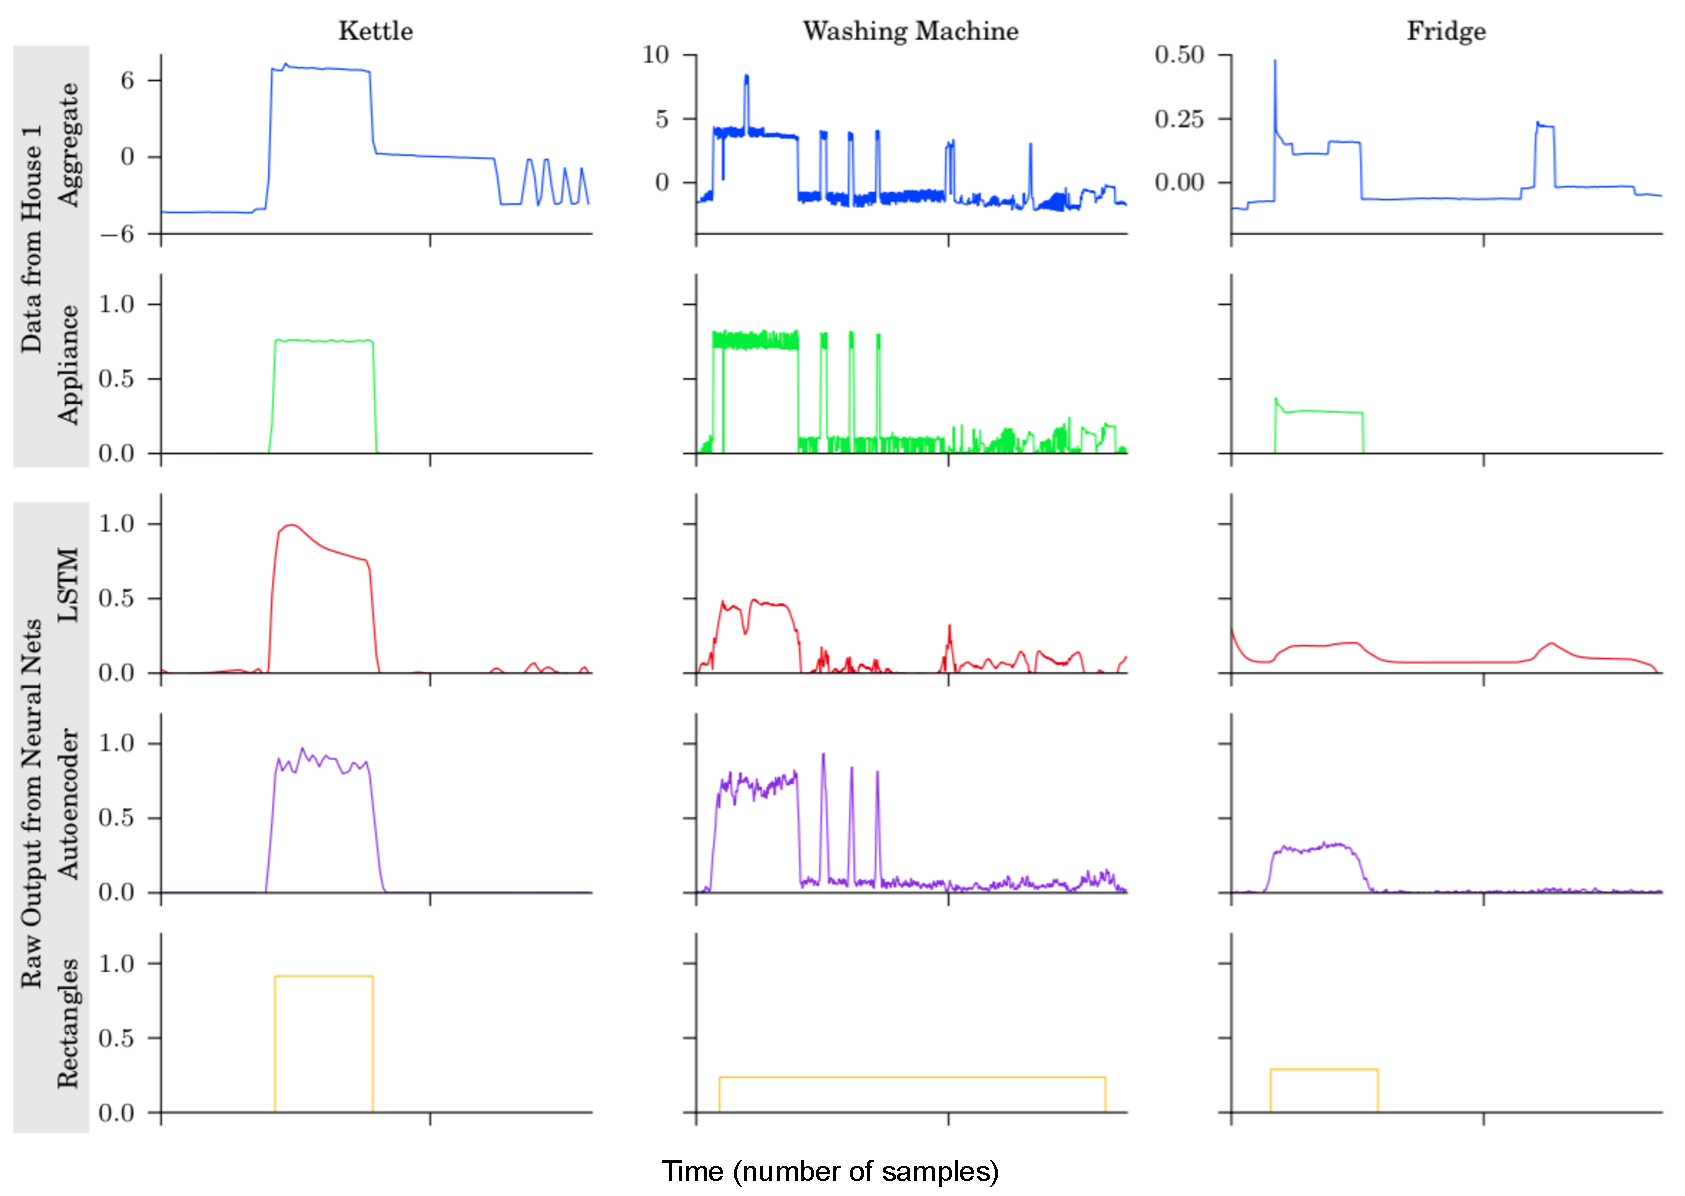
\includegraphics[width=1\textwidth]{./chapters/chapter2/images/neuralNILM.pdf} 
\caption{Outputs produced by three deep neural networks~\cite{KellyK15}.} 
\label{fig:AA4} 
\end{figure}

Besides ANN, HMM is also applied to find the state of devices in NILM~\cite{Parson12,Kim11ICDM,Kolter11redd,Nambi13,Lukaszewski13,Zoha13,Jia15,Ridi14}. The state of each device can be considered as a hidden variable, while the observations relate to the aggregate power consumption. In~\cite{Parson12}, the aggregate power consumption $x$ as well as the difference on the power between two consecutive time slices, denoted as $y=x_i-x_{i-1}$, are considered as the observations of a so-called difference HMM, as represented in Figure~\ref{fig:A11}, to find the state sequence $s$ of the devices.
\begin{figure}
\centering
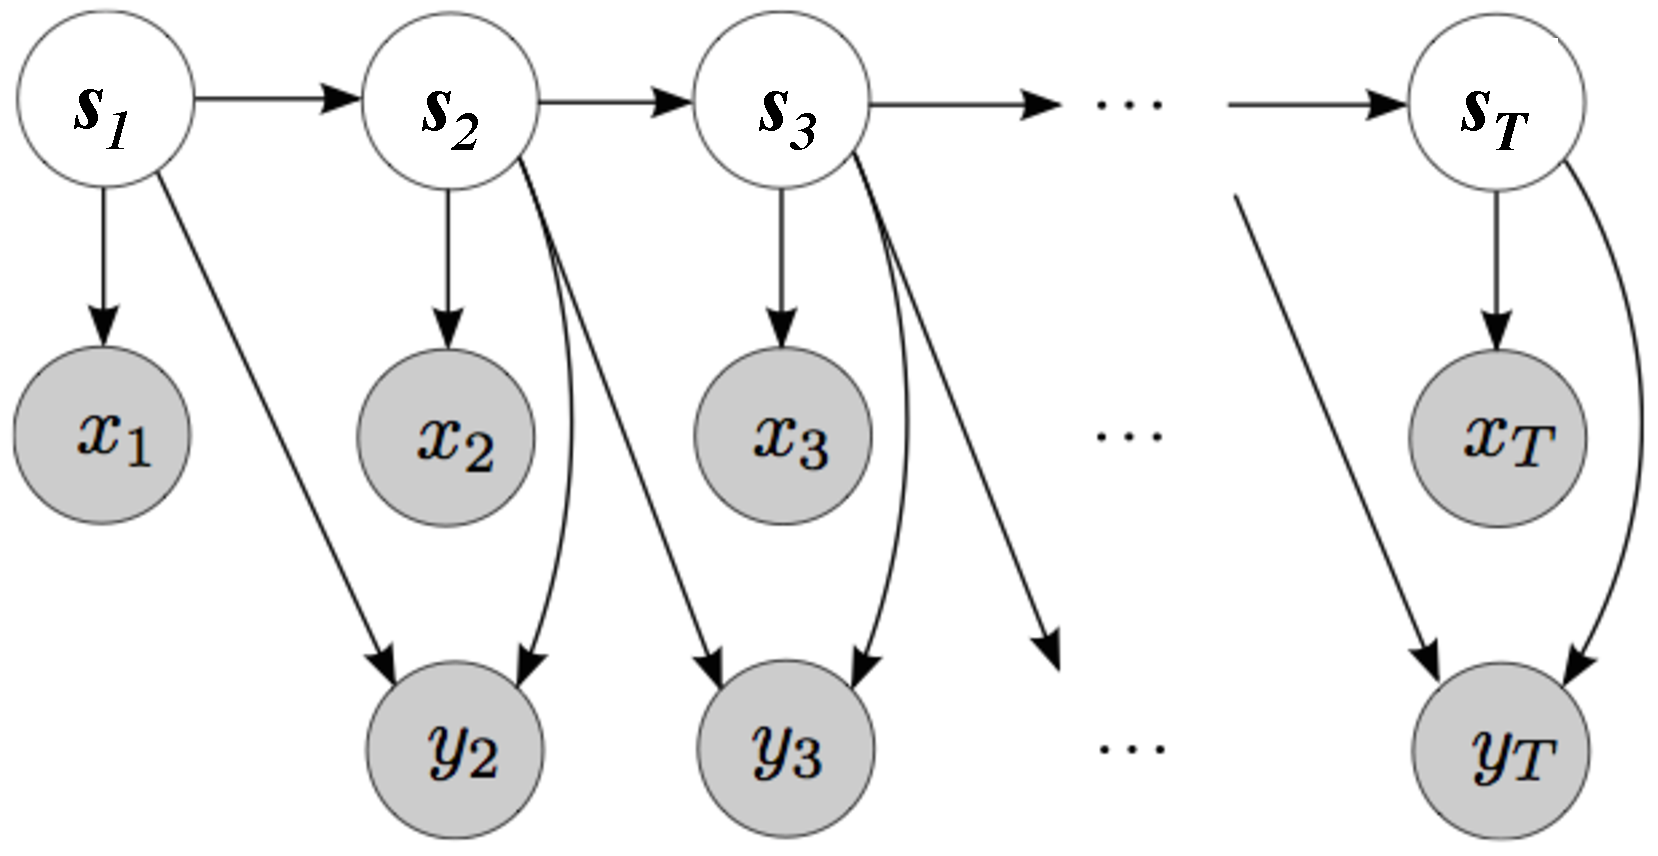
\includegraphics[width=0.5\textwidth]{./chapters/chapter2/images/HMM.pdf} 
\caption{Difference HMM~\cite{Parson12}. Shaded nodes represent the observations and unshaded nodes represent the hidden variables.} 
\label{fig:A11} 
\end{figure}
The correlation of the variables in this model are defined by a set $\theta$ of three parameters learned from the training dataset 
\begin{equation}
\theta = \{\pi ,\mathbf{A},\phi\},
\end{equation}
where $\pi$ denotes the probability of the initial state, $\mathbf{A}$ the transition probability matrix from a state at time $(t-1)$ to another at time $t$ and $\phi$ the emission probability generated by a state and assumed to follow the Gaussian distribution. Besides, a constraint that a device is only in on-state if the aggregate power is larger than its own power demand is also necessary to be imposed.
The state of each device is determined by applying the extension of Viterbi algorithm through two steps. In the first step, a filter is applied to suppress the observations whose joint probability does not excess the predefined threshold and the second step evaluates the joint probability of all sequences $x$, $y$, $s$ to identify the state of devices is defined as
\begin{equation}
\begin{split}
p(x,y,s|\theta)=p(s_1|\pi)\prod_{t=2}^{T}{p(s_t|s_{t-1},\mathbf{A})}
\prod_{t=1}^{T}{P(w_{s_t}\leq x_t|s_t,\phi)}\prod_{t\in S}{p(y_t|s_t,s_{t-1},\phi)},
\end{split}
\end{equation}
where $S$ is the set of filtered observations and $T$ is the length of observation sequence.

Meanwhile, in~\cite{Kim11ICDM}, only the aggregate power consumption is considered as observation sequence. In this research, the on-duration of home devices can be modeled as following the gamma distribution with a couple of parameters $\kappa^{(i)}$, $\theta^{(i)}$ for each device $i$. This assumption is drawn from the on-duration histogram of some popular electrical devices such as television, laptop, monitor, etc. as shown in Figure~\ref{fig:AA12}. Moreover, some additional features such as time of day, day of week and environment information from a monitoring sensors network are also taken into account. Considering $K$ additional conditions with corresponding sequences $c^{(1)}, \ldots, c^{(K)}$ in HMM creates a Conditional Factorial Hidden Semi-Markov Model (CFHSMM) and is illustrated by the graphical model in Figure~\ref{fig:A12}. 

\begin{figure}
\centering
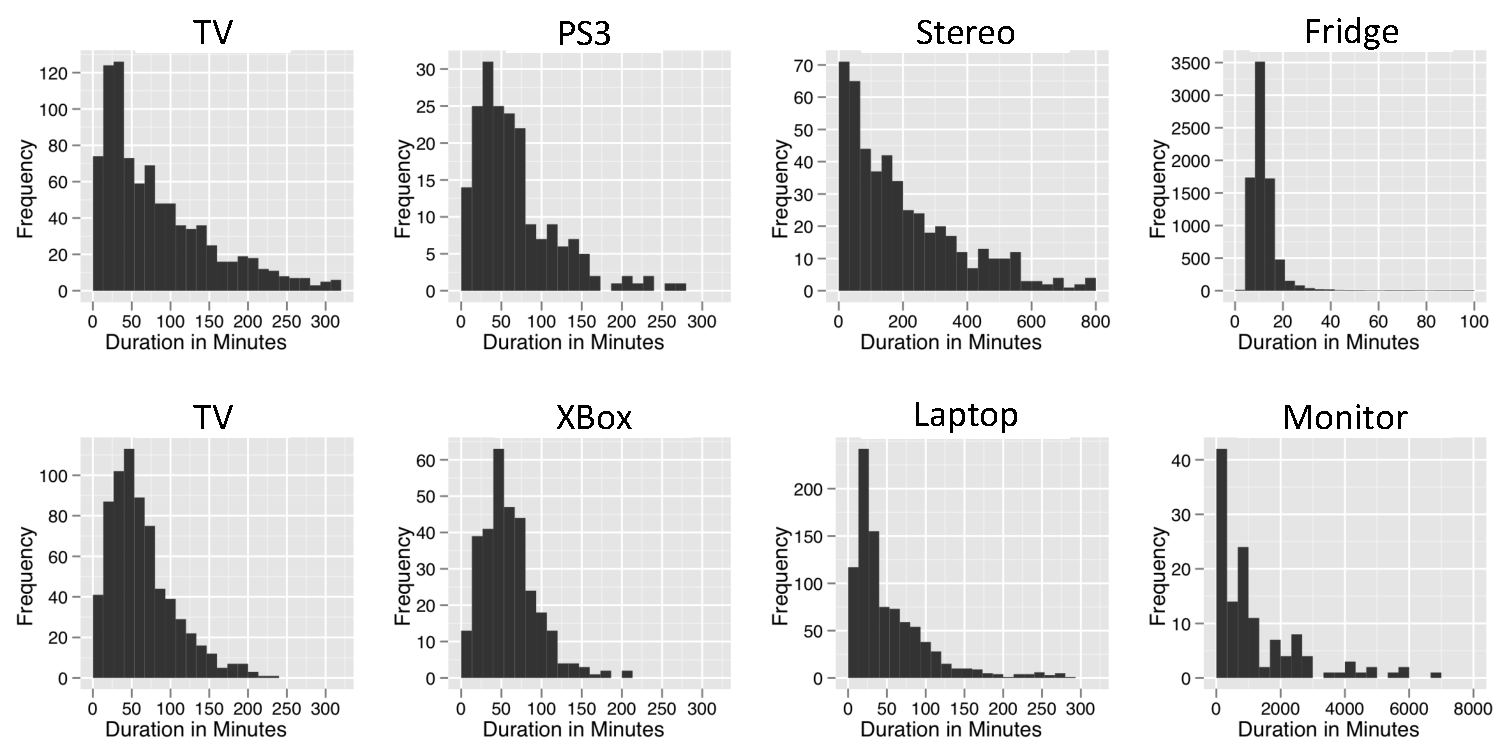
\includegraphics[width=1\textwidth]{./chapters/chapter2/images/on-duration_gamma.pdf} 
\caption{On-duration histogram of some devices~\cite{Kim11ICDM}.} 
\label{fig:AA12} 
\end{figure}

\begin{figure}
\centering
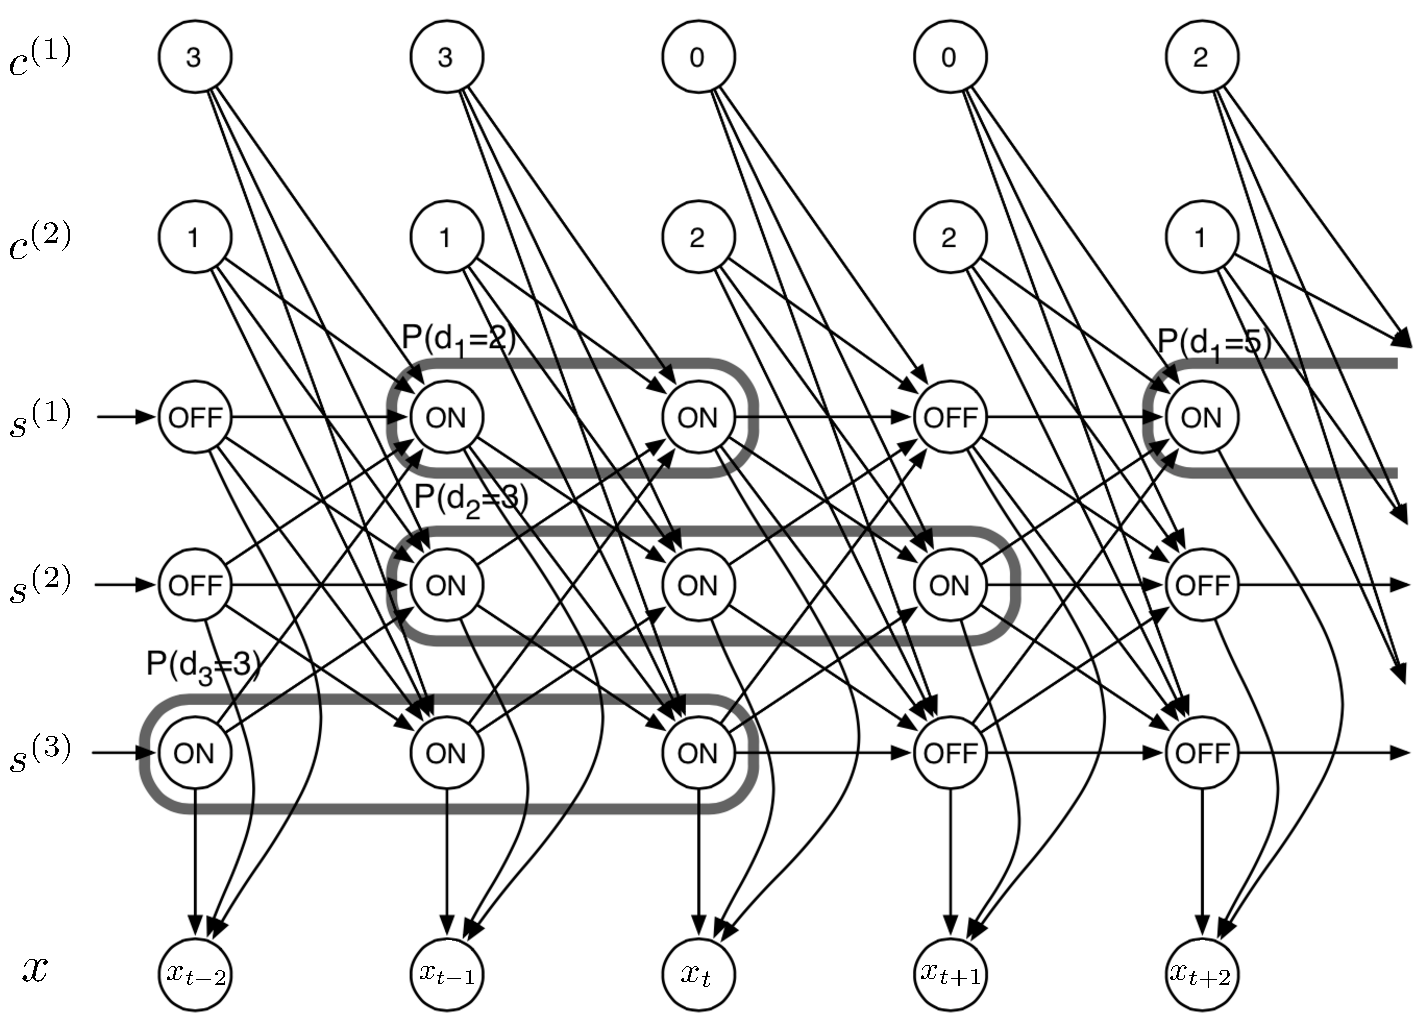
\includegraphics[width=.8\textwidth]{./chapters/chapter2/images/CFHSMM.pdf} 
\caption{Graphical representation of CFHSMM with the additional conditions $c^{(1)}$, $c^{(2)}$~\cite{Kim11ICDM}.} 
\label{fig:A12} 
\end{figure}

The hidden variables $s^*$ of this model can be found by applying the Maximum Likelihood Estimation (MLE) after training the set of parameters $\lambda$,
\begin{equation}
s^*=\argmax_{s}{P(X,s|\lambda)},
\end{equation}
where $P(X,s|\lambda)$ is the joint probability computed by the product of the initial probability $\psi_{in}(X,s|\lambda)$, the emission probability $\psi_e(X,s|\lambda)$, and the transition probability $\psi_t(X,s|\lambda)$, i.e.,
\begin{equation}
P(X,s|\lambda)=\psi_{in}(X,s|\lambda)\times \psi_e(X,s|\lambda)\times \psi_t(X,s|\lambda).
\end{equation}
The difference of this model compared to other HMMs is the consideration of external information in estimating the transition probability, as follows:
\begin{equation}
\begin{split}
\psi_t(X,s|\lambda)=&\prod_{i=1}^{N}{\prod_{t:s_t^{(i)}=0}{\left(\left(\prod_{j=1}^N{m_{s_{t+1}^{(i)}js_t^{(j)}}^{(i)}} \right) \left(\prod_{j=1}^K{f_{s_{t+1}^{(i)}jc_t^{(j)}}^{(i)}}\right)\right)}}\\
&\prod_{t:s_t^{(i)}=1}{\left(\left(\prod_{j=1:i\neq j}^N{m_{s_{t+1}^{(i)}js_t^{(j)}}^{(i)}} \right)\left(\prod_{j=1}^K{f_{s_{t+1}^{(i)}jc_t^{(j)}}^{(i)}}\right)\right)}\\
&\prod_{t:s_t^{(i)}=1,s_{t-1}^{(i)}=0}P(d=l_t^{(i)}|\kappa^{(i)},\theta^{(i)}),
\end{split}
\end{equation}
where $m_{kjl}^{(i)} = P(s_{t}^{(i)}=k|s_{t-1}^{(j)}=l)$ is the conditional probability for device $j$ of state $l$, $f_{kjl}^{(i)} = P(s_{t}^{(i)}=k|c_{t-1}^{(j)}=l)$ is the conditional probability for external feature $j$ of value $l$, $d$ is the on-duration length and $l_t^{(i)}$ is the length of on-duration of device $i$ beginning from time $t$.

Another less complex model of CFHSMM also applied in NILM is the Factorial Hidden Markov Model (FHMM) \cite{Kolter11redd,Nambi13,Lukaszewski13,Zoha13,Jia15}, in which the states of each device are considered as a hidden sequence and the external information is ignored. In those researches, we can find a Nonparametric Factorial Hidden Markov Model~\cite{Jia15}, which helps to eliminate the need of sub-metered data to train the model or the prior knowledge about the number of devices. Nevertheless, detecting the devices with many levels of power demand is a challenge. Constructing the problem in the context of NILM as an HMM can give an effective state determination approach for low-frequency power measurement. It helps to improve the accuracy and opens many perspectives to develop in future work. The accuracy of this method varies depending on the type and number of devices. Nevertheless, this approach has some limitations such as excessive training period to consider the distribution of the variables as well as complexity computation.







\subsection{Optical Network Interface}\label{micro}

In many cases, low-frequency based algorithms cannot discern the devices with the same power characteristics such as power demand, operating duration, rising and falling edges, etc. Besides, if a device consumes a variable energy over time, the steady state does not exist and the detection algorithm cannot accurately execute. Therefore, studies on other algorithms based on a higher sampling frequency are necessary. These algorithms will focus on harmonics and especially transient phase, which contains much useful information about the devices.

\begin{figure}[!ht]
\centering
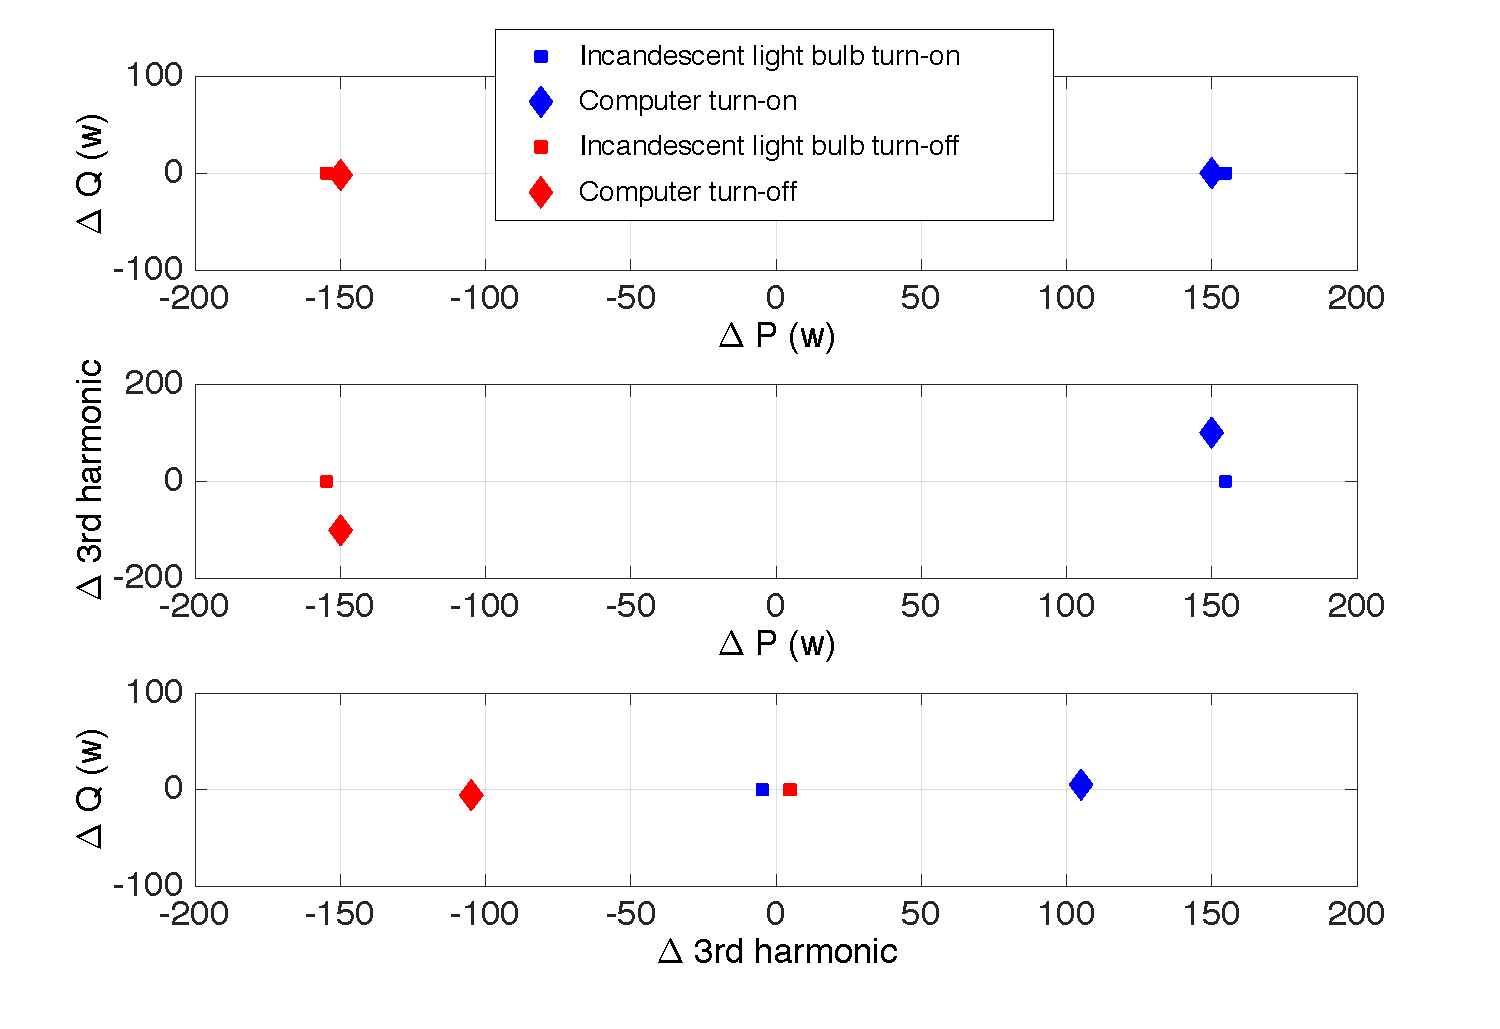
\includegraphics[width=0.8\textwidth]{./chapters/chapter2/images/third_harmonic_discrimination.pdf} 
\caption{A computer and an incandescent light bulb cannot be discriminated by the real and reactive power but can be distinguished by analyzing the third harmonic~\cite{Laughman03PEM}.} 
\label{fig:A14} 
\end{figure}
In \cite{Liang10I,Liang10II,Laughman03PEM,Cole2000,Suzuki08,Li12}, the authors propose to use the Fourier transform to determine the current harmonics. In~\cite{Laughman03PEM}, the indistinguishable problem of the devices consuming the same power in~\cite{Hart92} is solved by using the third harmonic obtained from the phase-locked short-time Fourier transform of current waveform collected at 8000~Hz and higher sampling frequency. As shown in Figure~\ref{fig:A14}, an incandescent light bulb and a computer cannot be discriminated by the first harmonics, i.e. real and reactive power, but can be distinguished by analyzing the third harmonics. Additionally, as presented in~\cite{Laughman03PEM}, the operating devices can also be detected by matching the events on the transient phase with the predefined signatures obtained from the training period. For example, the transient phases of a computer and an incandescent lamp are distinguishable because heating a lamp filament is different from charging the power supply or the batteries of a computer. Furthermore, transient-based recognition also allows near-real-time identification of energy consumers.
That is the reason why the transient signal is studied in many other researches \cite{Shaw08,Cox06,Yang07,Lin10,Chang11, Leeb95PD,Chang08,Lee05,Wichakool09,Chang12}.

In \cite{Shaw08,Cox06}, short-time Fourier transform is used to compute the spectral envelope coefficients of the transient signal when starting a device. The electrical load transients detected by the system will be classified by comparing with the existing transient signatures in the library.
In contrast, the authors of \cite{Yang07,Lin10,Chang11} try to apply an ANN to process the transient signal. In \cite{Yang07}, the transient period is segmented into windows and a wavelet transform is applied to each one. Meanwhile, the load current acquisition can be measured instead of power consumption to reduce the complexity and computation~\cite{Lin10}. ANN can also be combined with a genetic algorithm to identify load demands and improve recognition accuracy of NILM results~\cite{Chang11}. 

However, detecting complete transient shapes is sometimes a waste of memory and not necessary. That is the reason why in~\cite{Leeb95PD}, the authors introduce a new time pattern called \textit{v-shape}, which is the periods containing the significant changes during the transient phase. Figure~\ref{fig:A15} shows an example of the \textit{v-shapes} in the transient signal of an induction motor. The principle of \textit{v-shape}-based identification is to search for the precise time pattern of \textit{v-shape} and compare with the existing patterns in the library.
\begin{figure}[!ht]
\centering
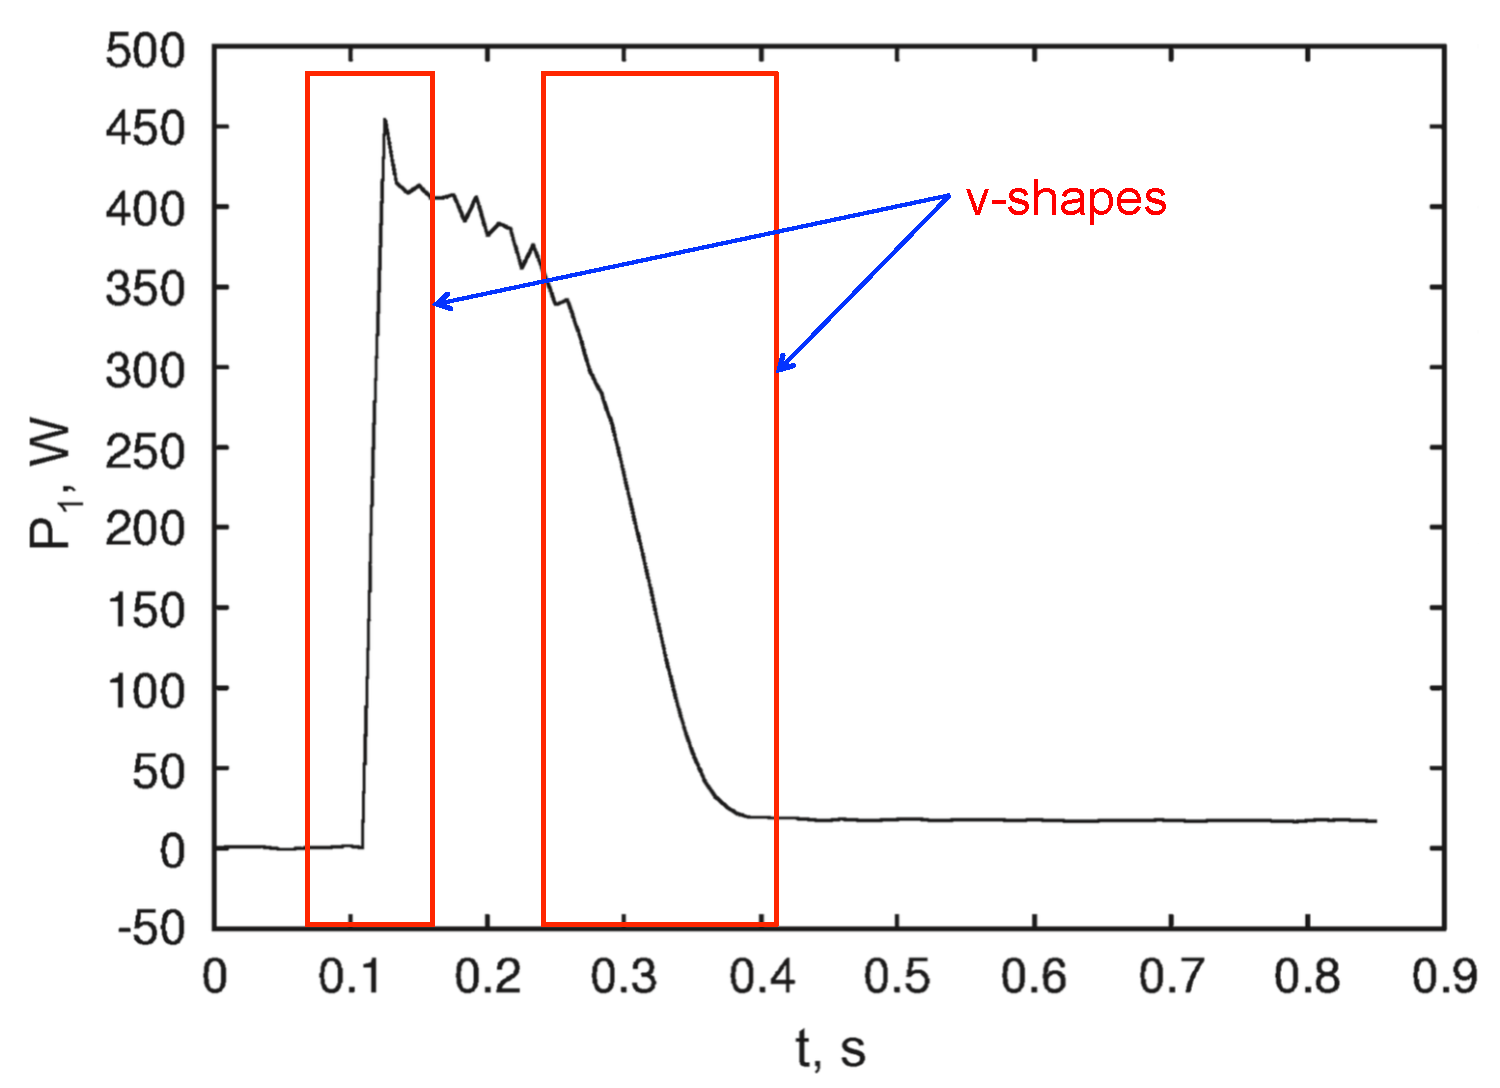
\includegraphics[width=0.6\textwidth]{./chapters/chapter2/images/v-shape.pdf} 
\caption{\textit{v-shapes} on the transient of an induction motor~\cite{Leeb95PD}.} 
\label{fig:A15} 
\end{figure}


A limitation of the transient-based algorithms relates to the simultaneous operation in which two or more devices are switched on at the same time. To overcome this restriction, in~\cite{Srinivasan06PD}, Fast Fourier Transform (FFT) is applied to analyze the harmonics of the incoming current waveform. Both real and imaginary parts of the harmonics are the inputs of an ANN, in which the number of inputs depends on the effectiveness of the additional harmonics, while the number of outputs relates to the number of classes, i.e. number of known devices. Figure~\ref{fig:A16} represents the mean value and standard deviation of the harmonics of some typical devices.
\begin{figure}
\centering
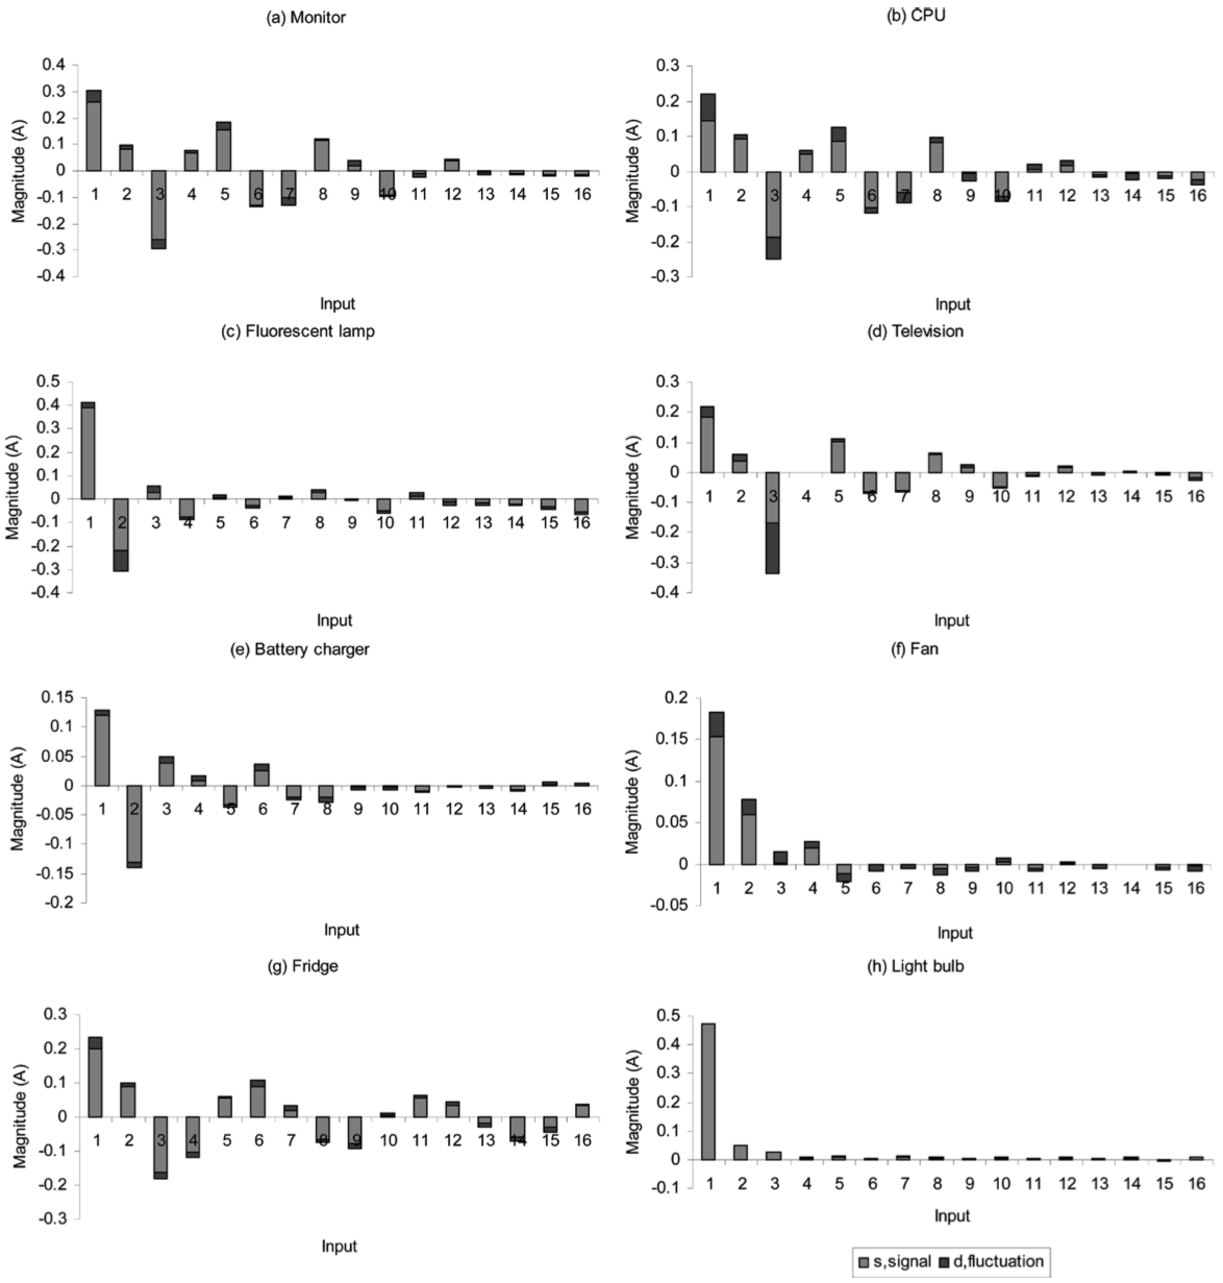
\includegraphics[width=1\textwidth]{./chapters/chapter2/images/harmonic_of_devices.pdf} 
\caption{Harmonic signatures of typical devices~\cite{Srinivasan06PD}.} 
\label{fig:A16} 
\end{figure}

Besides analyzing the spectral and harmonic content, a novel method using V-I trajectory to categorize the groups of devices is also proposed in \cite{Lee04,Lam07}. The V-I trajectory is plotted for each device using the normalized current and voltage values. Figure~\ref{fig:A17} illustrates an example of the voltage and current waveforms of a television and the corresponding V-I trajectory. This method can form a high performance due to the distinctive V-I curves of devices. However, it is sensitive to the operation scenario of the multi-state loads. Moreover, the trajectory patterns of small loads are difficult to be distinguished.

\begin{figure}
\centering
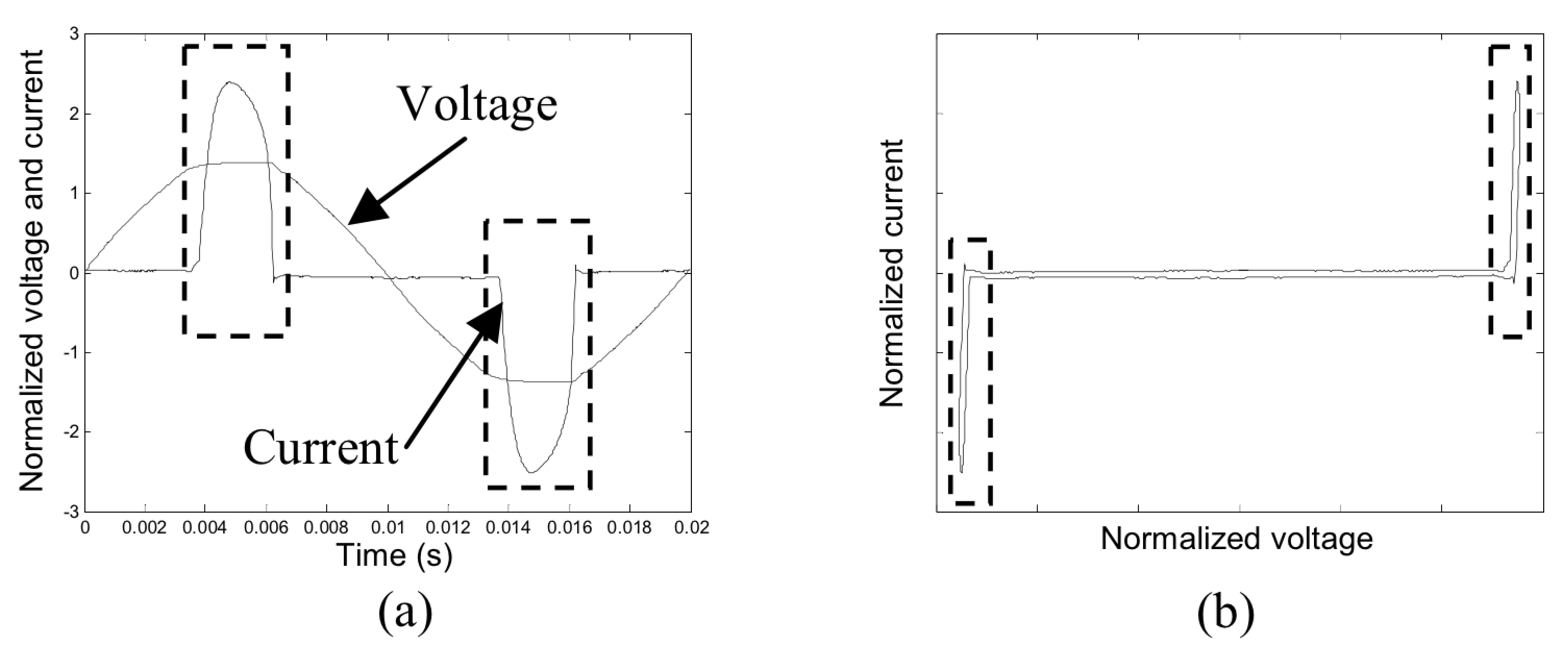
\includegraphics[width=0.9\textwidth]{./chapters/chapter2/images/VItrajectory.pdf} 
\caption{(a) Current and voltage waveforms of a television. (b) Corresponding V-I trajectory~\cite{Lam07}.} 
\label{fig:A17} 
\end{figure}

In another research, the authors of~\cite{Gupta10} introduce a new approach to identify the running devices by detecting the noise created on the monitored power line, based on a high frequency hardware and 2048-point FFT. In homes and buildings, there are some devices running on background and their power waveform is detected and saved on the memory. Whenever a new device is turned on, a noise is created on the background and the respective new device can be identified by analyzing the frequency components of the measured signal. For example, Figure~\ref{fig:A18} shows the new signal appearing on the background noise and its extracted frequency components. 
\begin{figure}
\centering
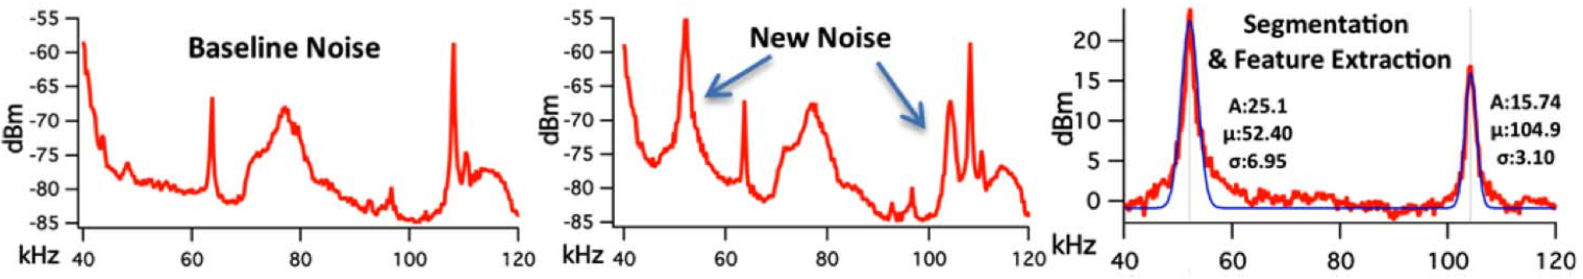
\includegraphics[width=1\textwidth]{./chapters/chapter2/images/noiseEMI.pdf} 
\caption{New noise feature extracted from the background noise~\cite{Gupta10}.} 
\label{fig:A18} 
\end{figure}

Similarly, a system called Detecting Operating States of Electronic devices (DOSE)~\cite{Chen15} tries to detect the variation on the electromagnetic field to identify the corresponding devices. The Electromagnetic Interference (EMI), generated when an electronic device operates, is coupled to the power line and its form is picked up by a sensing hardware attached to the outlet. As shown in Figure~\ref{fig:A19}, the time-varying EMI of a laptop is different and distinguishable at idle, medium load and high load.

\begin{figure}
\centering
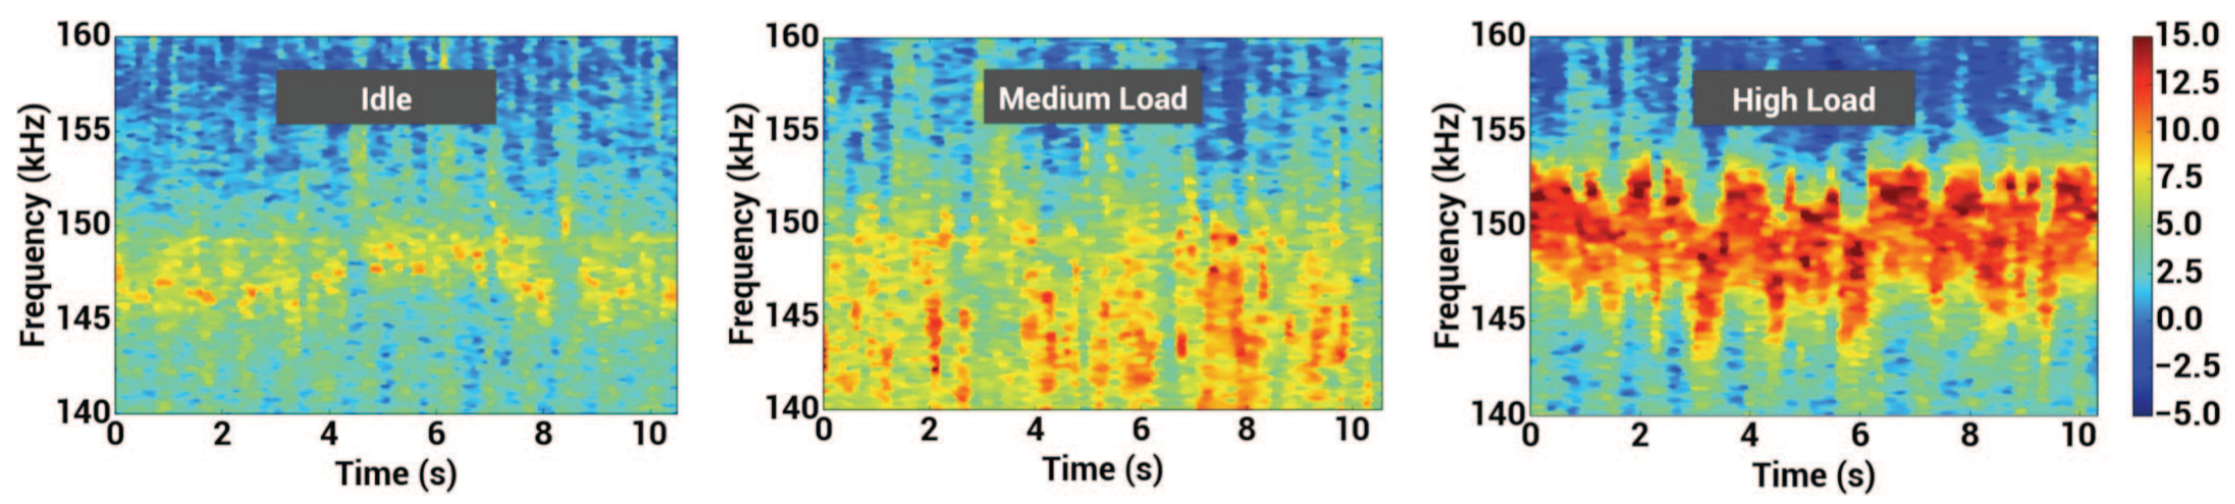
\includegraphics[width=1\textwidth]{./chapters/chapter2/images/DOSE.pdf} 
\caption{Time-varying EMI of a laptop at idle, medium load and high load~\cite{Chen15}.} 
\label{fig:A19} 
\end{figure}
Although high-frequency based methods show a perspective to significantly improve device identification, the most important drawback preventing it from being widely implemented is the deployment cost, which increases along with the frequency of hardware.
\lhead{\emph{State of the Art}}
\section{State-of-the-art of Error Correction Code}
\subsection{Related works}
\subsection{ECC for Optical Interconnects}

Instead of deploying a WSN to monitor all devices in home as in ILM, a hybrid system uses less sensors to detect the environmental parameters and infer the state of some specific devices, while the others are still identified by an NILM algorithm. 
In order to reduce the computational complexity while still ensuring the accuracy for load monitoring, in \cite{TangW16}, the occupancy is considered as a significant external feature because a part of devices operates during occupied periods. Figure~\ref{fig:A13} illustrates the correlation between the operation of some devices and the occupancy in home. Therefore, the NILM algorithms can be applied only when the occupancy monitoring system, as introduced in Chapter \ref{Introduction}, detects an occupancy. By cutting out the unoccupied periods, the computational complexity can significantly decrease, particularly if the unoccupied periods are dominating. Obviously, the detection accuracy also decreases if there are too many background loads or automatically fluctuated devices such as fridge, washing machine, dish washer, heater, etc. Meanwhile, in \cite{Berges10,Berges11,Guvensan13}, the environmental parameters such as light intensity or audio signal are analyzed to give conclusion on the operation of some specific devices, e.g. the variations in acoustic signal relate to the operation of an air blower and a refrigerator as shown in Figure~\ref{fig:AA13}. Instead of installing new sensors, the embedded sensors of mobile phones can also be used to fingerprint the profile of each device~\cite{Uddin12}. Although the hybrid approach allows to increase the performance of load monitoring systems, more algorithms must be studied for sensors signal processing.

\begin{figure}[!ht]
\centering
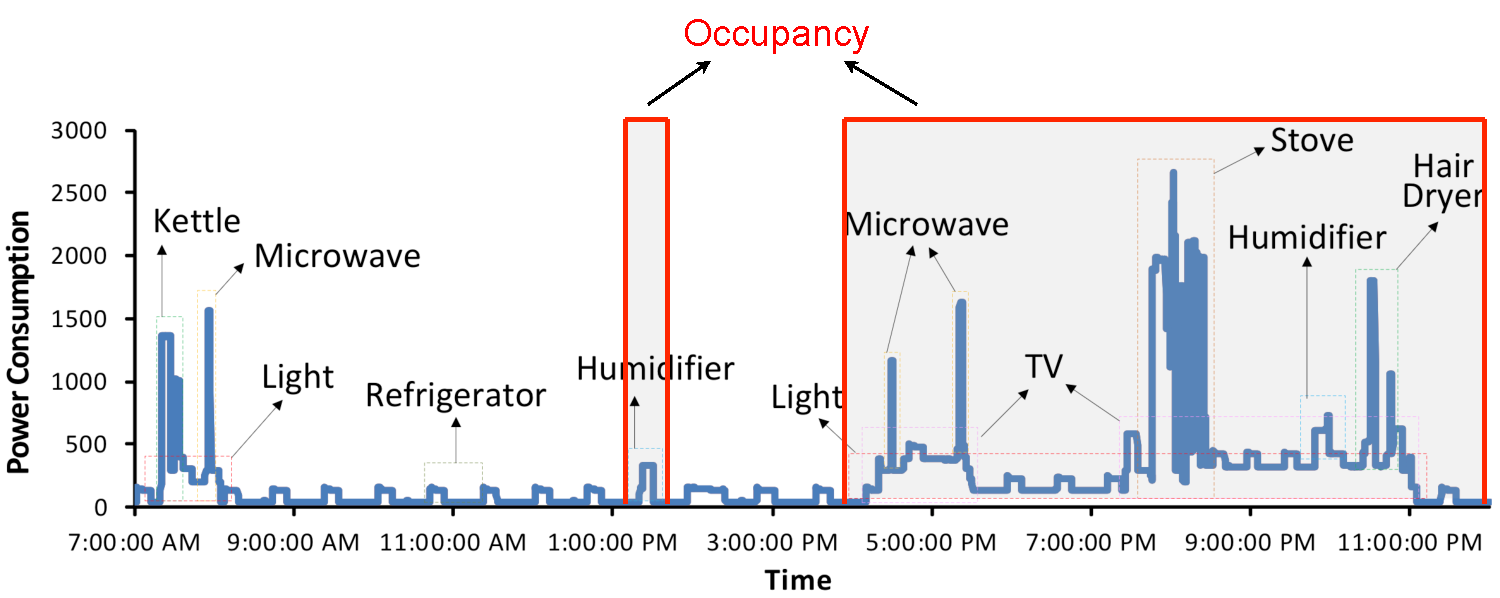
\includegraphics[width=1\textwidth]{./chapters/chapter2/images/occupancy_states.pdf} 
\caption{Power consumption with and without the occupants~\cite{TangW16}.} 
\label{fig:A13} 
\end{figure}

\begin{figure}[!ht]
\centering
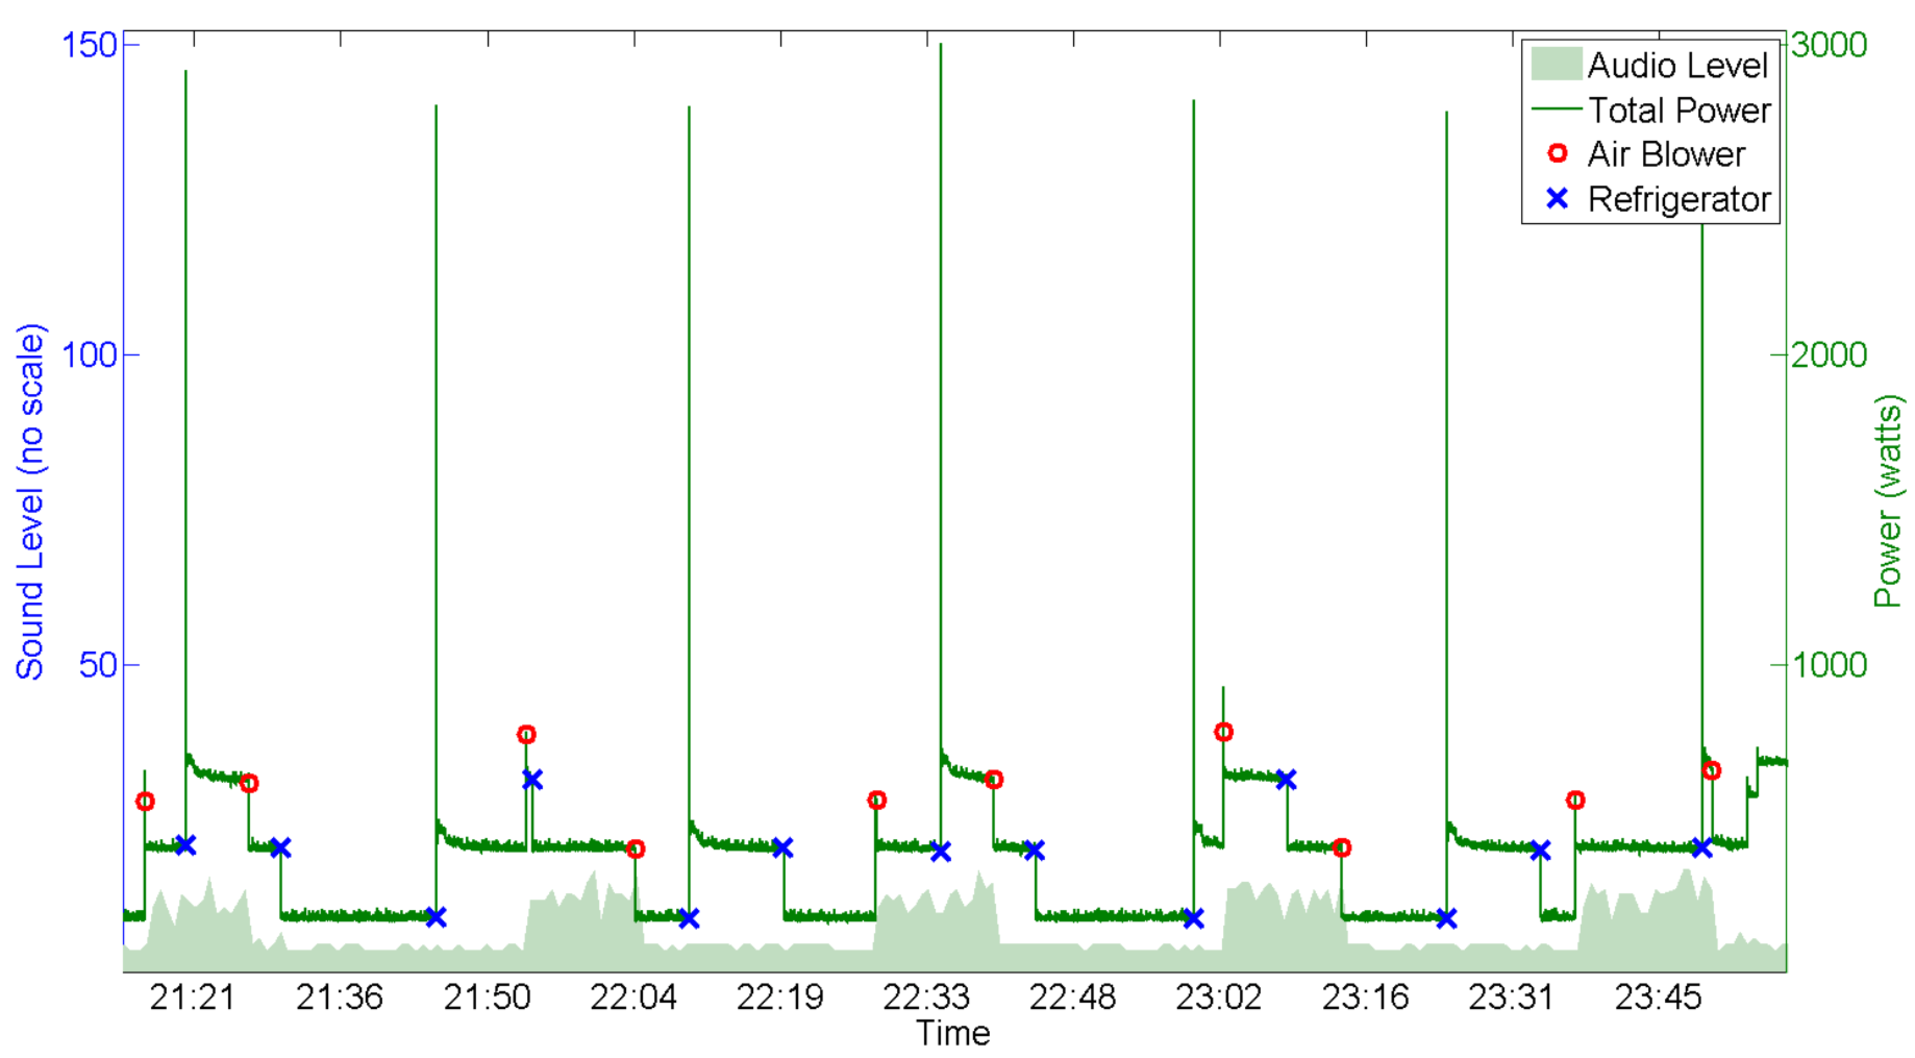
\includegraphics[width=1\textwidth]{./chapters/chapter2/images/audiochange.pdf} 
\caption{Aggregate power consumption and the variation of audio signal in a living room~\cite{Berges10}.} 
\label{fig:AA13} 
\end{figure}



\section{Conclusions}
In this chapter, we have an overview on the load monitoring including intrusive, non-intrusive and hybrid approaches. ILM is the most accurate approach, but it needs very large amount of sensors to monitor all electrical consumers and therefore it is impossible to be widely applied. Meanwhile, non-intrusive approaches help to significantly reduce the deployment cost as well as technical intervention on the power supply. Nevertheless, ambiguity in the power characteristics of the devices is the most important problem in an NILM system and prevents the system from increasing the performance. As a consequence, HLM can be considered as a compromise between two approaches, which can reduce the deployment cost of ILM and increase the performance of NILM. In this thesis, we will study on hybrid methods, which use external information such as state transition probability or operating probability of each device to improve the performance of existing NILM algorithms. Concretely, in Chapter 3, we propose to use the state transition of each device from previous instant to current instant as an external information and combine it to the minimization problem in Eq.~\eqref{eqI7}. Meanwhile, in Chapter 4, we introduce SmartSense model, in which a WSN is deployed to monitor the operation of a subset of all devices. Sensor detection is then transformed to the operating probability of corresponding devices. Disaggregation algorithms use this probability along with other specific features extracted from the global power signal to determine the state of each device.


























% Chapter 4

\chapter{Modeling and analyzing of attenuation in optical interconnects} % Write in your own chapter title
\label{l1norm}
%\addtotoc{State of the Arts}
\lhead{\emph{Algorithms for NILM based on $l1$-norm Minimization}} % Write in your own chapter title to set the page header

In this chapter, we try to solve the $l1$-norm minimization problem in Eq.~\eqref{eqI7} defined in Section~\ref{nilm} by brute force approach, also called Least Absolute Error (LAE) based algorithm. Thereby, all possible combinations of states will be sequentially tested and the most suitable one will be selected as solution. However, because of the ambiguity on power demand of different devices, many combinations can give the same or near results, which reduces the algorithm accuracy. To improve performance, we propose to apply an additional information to select the solution among all possible combinations. This is a contribution to research on NILM. Two new methods are studied and introduced in this chapter. The first one, state difference-based algorithm, uses the Hamming distance between the possible combinations and the previous state of devices to find the solution for the $l1$-norm minimization problem, as introduced in Section~\ref{diff}. Meanwhile, the second one, called state transition probability-based algorithm and introduced in Section~\ref{proba}, considers the state transition probability from previous state to current state to determine the most suitable combination. The three proposed algorithms will be simulated in Matlab with data retrieved from a set of devices in our laboratory. Simulation results will be then compared with edge detection algorithm~\cite{Hart92}.
\section{Introduction}\label{LAE}
\section{Loss at device level}\label{LAE}
The $l1$-norm minimization problem for Equation~\eqref{eqI7} is presented as follows:
\begin{eqnarray}\label{eqL1}
 &&\min_{\mathbf{s}}\parallel x(t)-\sum_{i=1}^{N}{\sum_{j=1}^{m_i}{s_{ij}(t)\times w_{ij}}}\parallel\\
\mbox{subject to:}&& s_{ij}(t)\in \{0,1\}, i=1,\ldots,N,j=1,\ldots,m_i\nonumber\\
&&\sum_{j=1}^{m_i}{s_{ij}(t)}\in \{0,1\}, i=1,\ldots,N. \nonumber
\end{eqnarray} 

To find the solution for problem \eqref{eqL1}, the conditions are at first processed by presenting all possible combinations of state vector $\mathbf{s}$ in matrix $\mathbf{S}$. Each row of $\mathbf{S}$ corresponds to a combination. For example, if there are two devices and each of them has two operation states, the state matrix $\mathbf{S}$ is defined as
\begin{equation*}
\mathbf{S}=\left[ \begin{array}{cccc}
0&0&0&0\\
0&0&0&1\\
0&1&0&1\\
0&1&0&0\\
0&1&1&0\\
0&0&1&0\\
1&0&1&0\\
1&0&0&0\\
1&0&0&1
\end{array}
\right]
\end{equation*}
Then, all combinations will be sequentially applied to the following equation to calculate the absolute error between the aggregate power and the total power demand of devices with corresponding state defined as
\begin{equation}\label{eqL2}
e(k) = |x(t) - \mathbf{s}^{(k)}\times \mathbf{w}^T|,
\end{equation}
where $e(k)$ is the absolute error corresponding to the combination $s^{(k)}$ in row $k$ of matrix $\mathbf{S}$. The combination giving the least value of $e(k)$ is selected as the solution. Therefore, this method is also called Least Absolute Error (LAE) based algorithm and presented in Algorithm~\ref{algoL1}. Obviously, the LAE based algorithm is exponentially complex and may be intractable with a large number of devices. However, it is considered in this chapter to study the performance improvement with the extrinsic information.

\begin{algorithm}
\caption{LAE-based algorithm for $l1$-norm minimization problem.}\label{algoL1}
\begin{algorithmic}[1]
\Function{LAEsolve}{$x,\mathbf{w}$}
\State Find all possible combinations of $\mathbf{s}$ and save in matrix $\mathbf{S}$
\State $l = \text{length}(x),x(0) = 0$
	\For {$t=1,\ldots,l$}
		\State $\mathbf{s} = \argmin_{\mathbf{s^{(k)}}\in \mathbf{S}}{|x(t) - \mathbf{s^{(k)}}\times \mathbf{w}^T|}$
		\State $ \mathbf{S_{out}}(t) = \mathbf{s}$
	\EndFor
	%\State \textbf{end for}
\State output = matrix $\mathbf{S_{out}}$
\EndFunction
%\State \textbf{end function}
\end{algorithmic}
\end{algorithm}







\section{Signal to noise ratio and model of loss at the system level}\label{diff}
In real condition, power consumption of a device is not stable. It can vary around an average value due to noise. In order not to leave out the true combination, it is necessary to retain the combinations giving an error closed to the least absolute error value and apply an additional constraint to select the solution: among all possible combinations, the final solution gives the smallest Hamming distance with the previous state. Hamming distance between two binary vectors is defined as the number of positions at which the corresponding values are different. 
A combination at row $k$ of $\mathbf{S}$ is retained if it satisfies the following condition:
\begin{equation}\label{eqL22}
\frac{|e(k)-e_{LAE}|}{e_{LAE}}\leq \gamma,
\end{equation}
where $e_{LAE}$ denotes the least absolute error and $\gamma$ is an empirically chosen threshold.
If this value is too small, the true solution of state vector $\mathbf{s}$ may be left out, while large value increases the number of retained combinations and the risk of error detection. Therefore, the selection of $\gamma$ needs to consider the standard deviation of the power consumption of devices as well as the difference between their power demand. Other combinations not satisfying condition \eqref{eqL22} will be ignored.
Finally, the combination having the smallest distance to the previous state is selected as the current state of devices, i.e.,
\begin{equation}
\mathbf{s} = \argmin_{\mathbf{s}\in \mathbf{S_C}}{|\mathbf{s}\oplus \mathbf{s}(t-1)|},
\end{equation}
where $\mathbf{S_C}$ is the set of combinations satisfying condition \eqref{eqL22}. The step-by-step procedure for state difference based method for $l1$-norm minimization problem is presented in Algorithm~\ref{algoL2}.
The retention of the combinations giving an absolute error close to the least one can prevent the algorithm from rejecting the accurate solution. However, this also increases the amount of computations to process the retained combinations, depending on the ambiguity level of the set of devices.

\begin{algorithm}
\caption{State difference based algorithm for $l1$-norm minimization problem.}\label{algoL2}
\begin{algorithmic}[1]
\Function{DIFFsolve}{$x,\mathbf{w}$,$\gamma$}
\State Find all possible combinations of $\mathbf{s}$ and save in matrix $\mathbf{S}$
\State $l = \text{length}(x),x(0) = 0,K=\text{length}(\mathbf{S})$
	\For{$t=1,\ldots,l$}
	    \For{$k=1,\ldots,K$}
	        \State $e(k) = |x(t)-s^{(k)}\times w^T|$
	    \EndFor
		\State $e_{LAE} = \min{\{e(i)|i=1,\ldots,K\}}$
		\State Find $\mathbf{S_C}\subset \mathbf{S}: \forall \mathbf{s^{(i)}}\in \mathbf{S_C},|e(i)-e_{LAE}|\leq \gamma \times e_{LAE}$
		\State $\mathbf{s} = \argmin_{\mathbf{s^{(i)}}\in \mathbf{S_C}}{\{|\mathbf{s^{(i)}}\oplus \mathbf{s}(t-1)|\}}$
		\State $\mathbf{S_{out}}(t) = \mathbf{s}$ 
	\EndFor
\State output = matrix $\mathbf{S_{out}}$
\EndFunction
%\State \textbf{end function}
\end{algorithmic}
\end{algorithm}





\subsection{Impact of crosstalk noise in loss}
\subsection{Impact of thermal issue in loss}\label{IoTherm}
Different from the previous algorithm, this method considers the state transition probability of each device to determine the current state instead of calculating the Hamming distance from all suitable combinations to the previous state of devices. Transition probability of each device, as shown in Figure~\ref{fig:L1}, is obtained from the training period. Based on condition \eqref{eqL22}, a subset of suitable combinations is retained and the coincidence probability for each one is calculated by the product of state transition probability of each element device, i.e.,
\begin{equation}\label{eqL5}
Pr(\mathbf{s}(t)|\mathbf{s}(t-1)) = \prod_{i=1}^{N}{p((s_i(t)|s_i(t-1))},
\end{equation}
where $p((s_i(t)|s_i(t-1))$ denotes the state transition probability of device $i$. The combination giving the largest probability will be selected to determine the current state of devices. Algorithm~\ref{algoL3} details the state determination in $l1$-norm minimization problem based on the state transition probability.
Similar to the state difference based algorithm, this method also needs more computations to calculate the coincidence transition probability of the retained combinations.

\begin{figure}
\centering
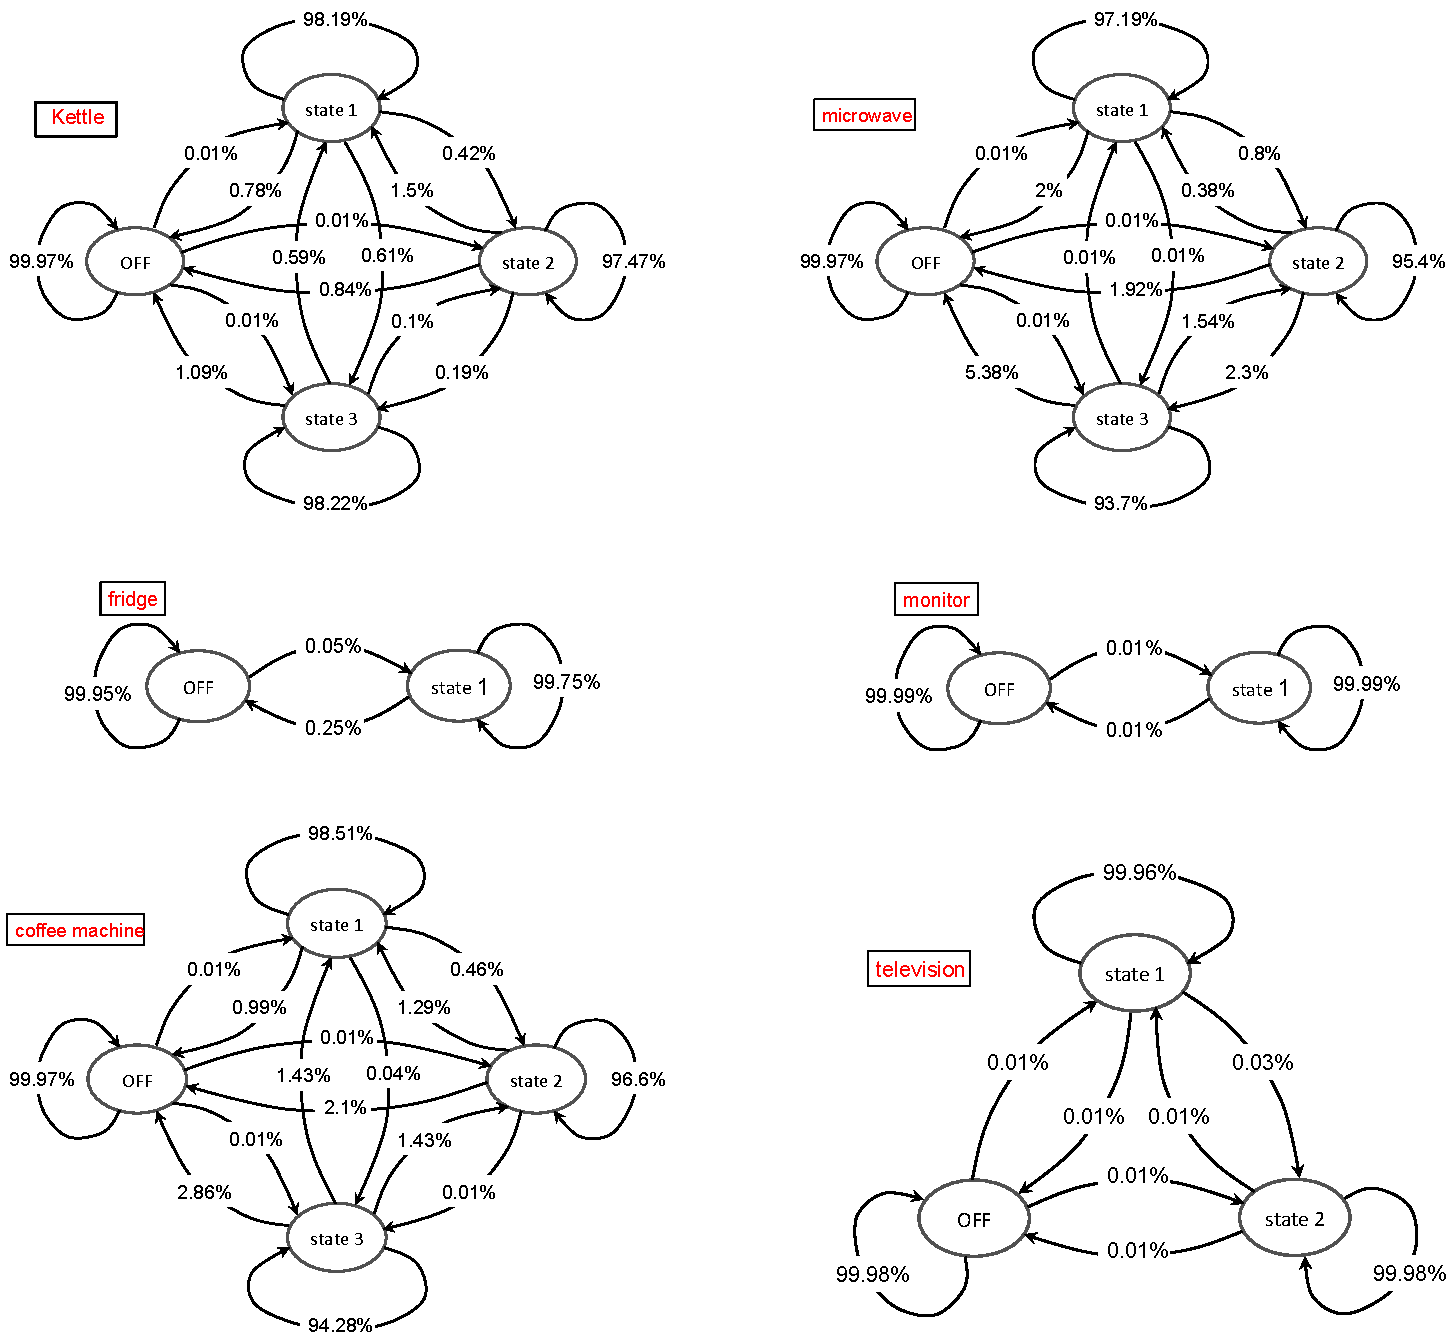
\includegraphics[width=1\textwidth]{./chapters/chapter3/images/Athemium_trans_proba.pdf} 
\caption{State transition probability of some devices in Athemium dataset obtained from a training period by attaching each of them to a power meter.} 
\label{fig:L1} 
\end{figure}

\begin{algorithm}
\caption{State transition probability based algorithm for $l1$-norm minimization problem.}\label{algoL3}
\begin{algorithmic}[1]
\Function{PROBsolve}{$x,\mathbf{w}$,$\gamma$}
\State Find possible combinations of $\mathbf{s}$ and save in matrix $\mathbf{S}$
\State $l = \text{length}(x),x(0) = 0,K=\text{length}(\mathbf{S})$
	\For {$t=1,\ldots,l$}
	    \For{$k=1,\ldots,K$}
	        \State $e(k) = |x(t)-s^{(k)}\times w^T|$
	    \EndFor
		\State $e_{LAE} = \min{\{e(i)|i=1,\ldots,K\}}$
		\State Find $\mathbf{S_C}\subset \mathbf{S}: \forall \mathbf{s^{(i)}}\in \mathbf{S_C},|e(i)-e_{LAE}|\leq \gamma \times e_{LAE}$
		\State $\mathbf{s} = \argmax_{\mathbf{s^{(i)}}\in \mathbf{S_C}}{\{Pr(\mathbf{s^{(i)}}|\mathbf{s}(t-1))\}}$
		\State $\mathbf{S_{out}}(t) = \mathbf{s}$
	\EndFor
\State output = matrix $\mathbf{S_{out}}$
\EndFunction
%\State \textbf{end function}
\end{algorithmic}
\end{algorithm}


\section{Simulation Results}
In this section, the three proposed algorithms for $l1$-norm minimization problem will be applied to our \emph{Athemium dataset} retrieved from a monitoring system presented in the next section. The performance of these algorithms will then be compared with the edge detection one~\cite{Hart92} to evaluate the improvement. Besides, they are also applied to detect the state of devices in the Reference Energy Disaggregation Dataset (REDD)~\cite{Kolter11redd}, one of the biggest publicly available dataset for NILM research community. In REDD, the power consumption in two main phases of electricity in six households in the USA is measured every second during many days and the power consumption of some typical devices is retrieved every 3-4 seconds.




%\subsection{The Worst-Case SNR in Chameleon ONoC}

\begin{figure}[h]
\centering
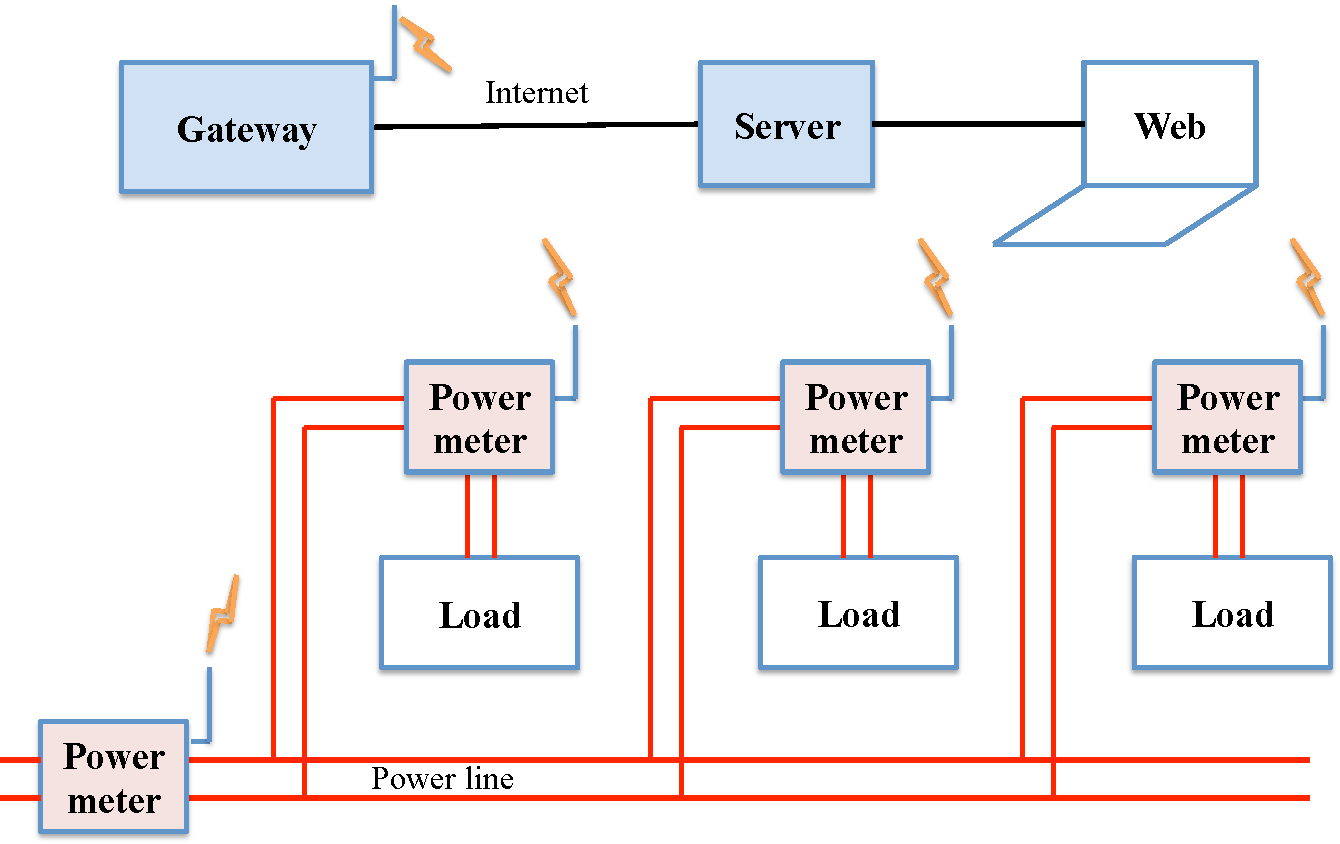
\includegraphics[width=.8\textwidth]{./chapters/chapter3/images/measurement_system.pdf} 
\caption{Smart meters network to retrieve the Athemium data.} 
\label{fig:L2} 
\end{figure}

To retrieve the Athemium data, a meter network supporting Zigbee wireless communications provided by Athemium company~\cite{Athemium} is deployed in the coffee room of our laboratory. 
The smart meter network is illustrated in Figure~\ref{fig:L2}, in which each device is attached to an individual meter. Data provided by these meters are used to learn the characteristics of each device as well as considered as ground truth data to evaluate performance of disaggregation algorithms. Additionally, a global power meter is also installed at the main circuit to measure the aggregate power consumption, which will be used to detect the operating states of each device. These power meters, fabricated by Netvox Technology Company~\cite{Netvok}, support wireless communication to send the power measurement to a gateway, which will forward it to an Athemium server through Internet connection. A web interface allows users to observe and download data. This interface lists all deployed power meters and sensors as well as their detailed parameters such as name, position, label, MAC address, as illustrated in Figure~\ref{fig:L22}. Besides, users can also display the power consumption of each device during hours, days, weeks, months and years.
\begin{figure}[htb]
\begin{minipage}[h]{1\linewidth}
\centering
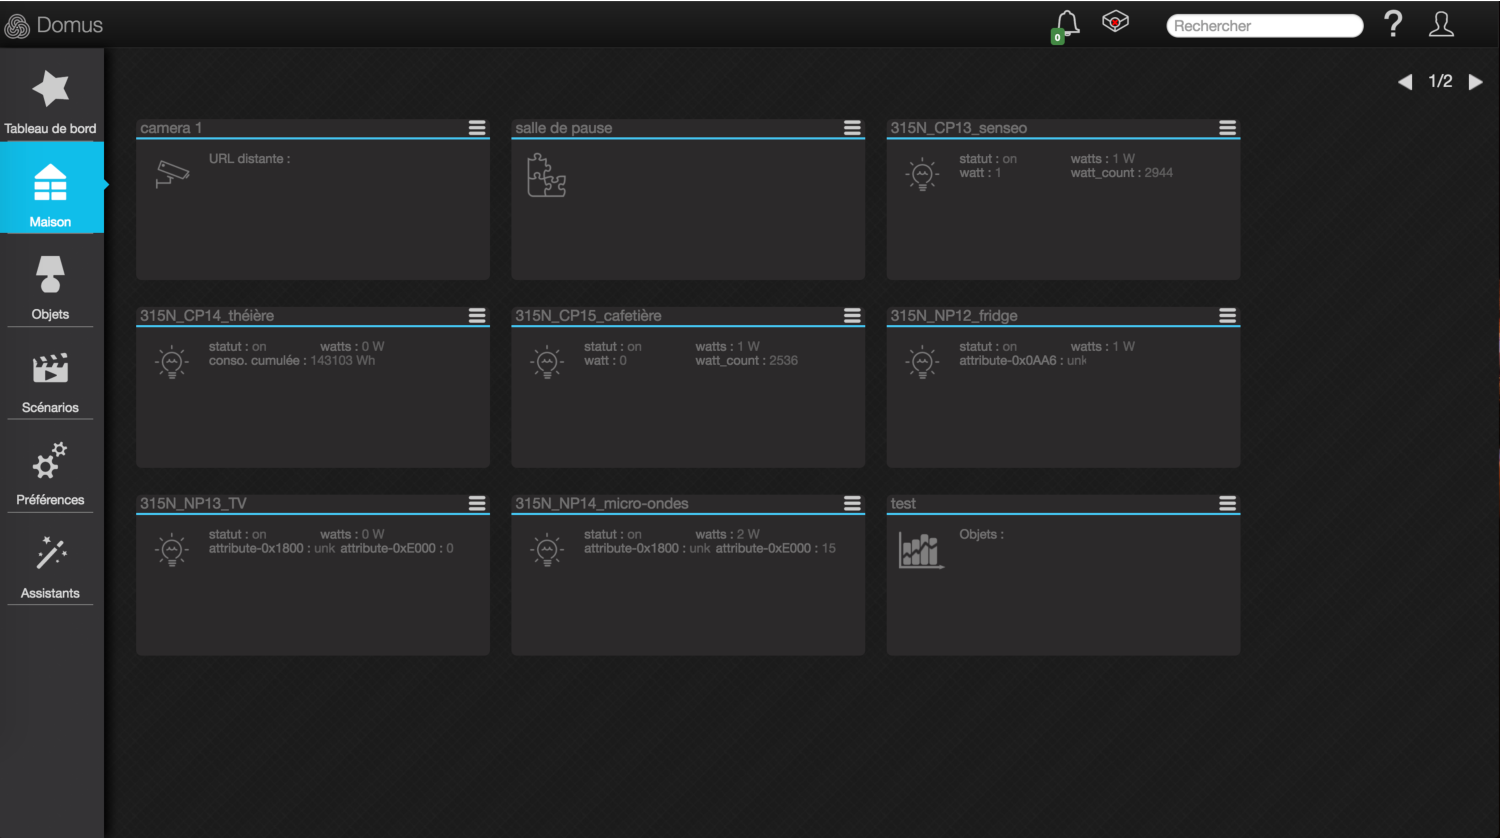
\includegraphics[width=0.8\textwidth]{./chapters/chapter3/images/A_web1.pdf}
%  \vspace{1.5cm}
\centerline{(a) List of deployed meters and sensors}\medskip
\end{minipage}
\hfill
\begin{minipage}[h]{0.48\linewidth}
\centering
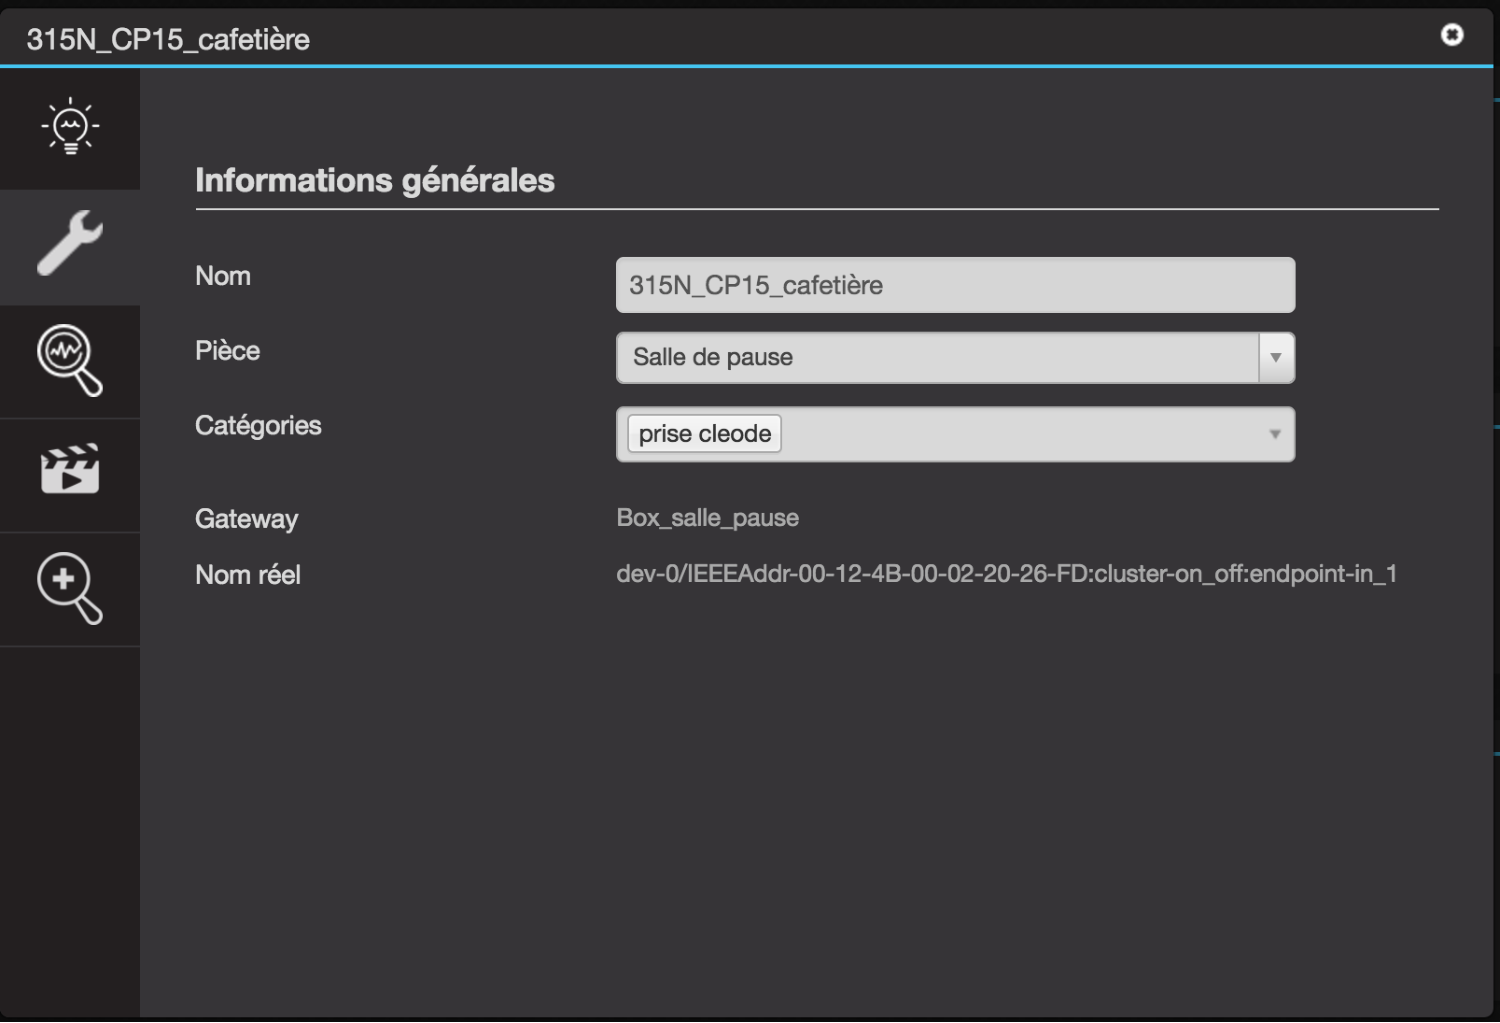
\includegraphics[width=1\textwidth]{./chapters/chapter3/images/A_web2.pdf}
%  \vspace{1.5cm}
\centerline{(b) Meters configuration}\medskip
\end{minipage}
\hfill
\begin{minipage}[h]{0.48\linewidth}
\centering
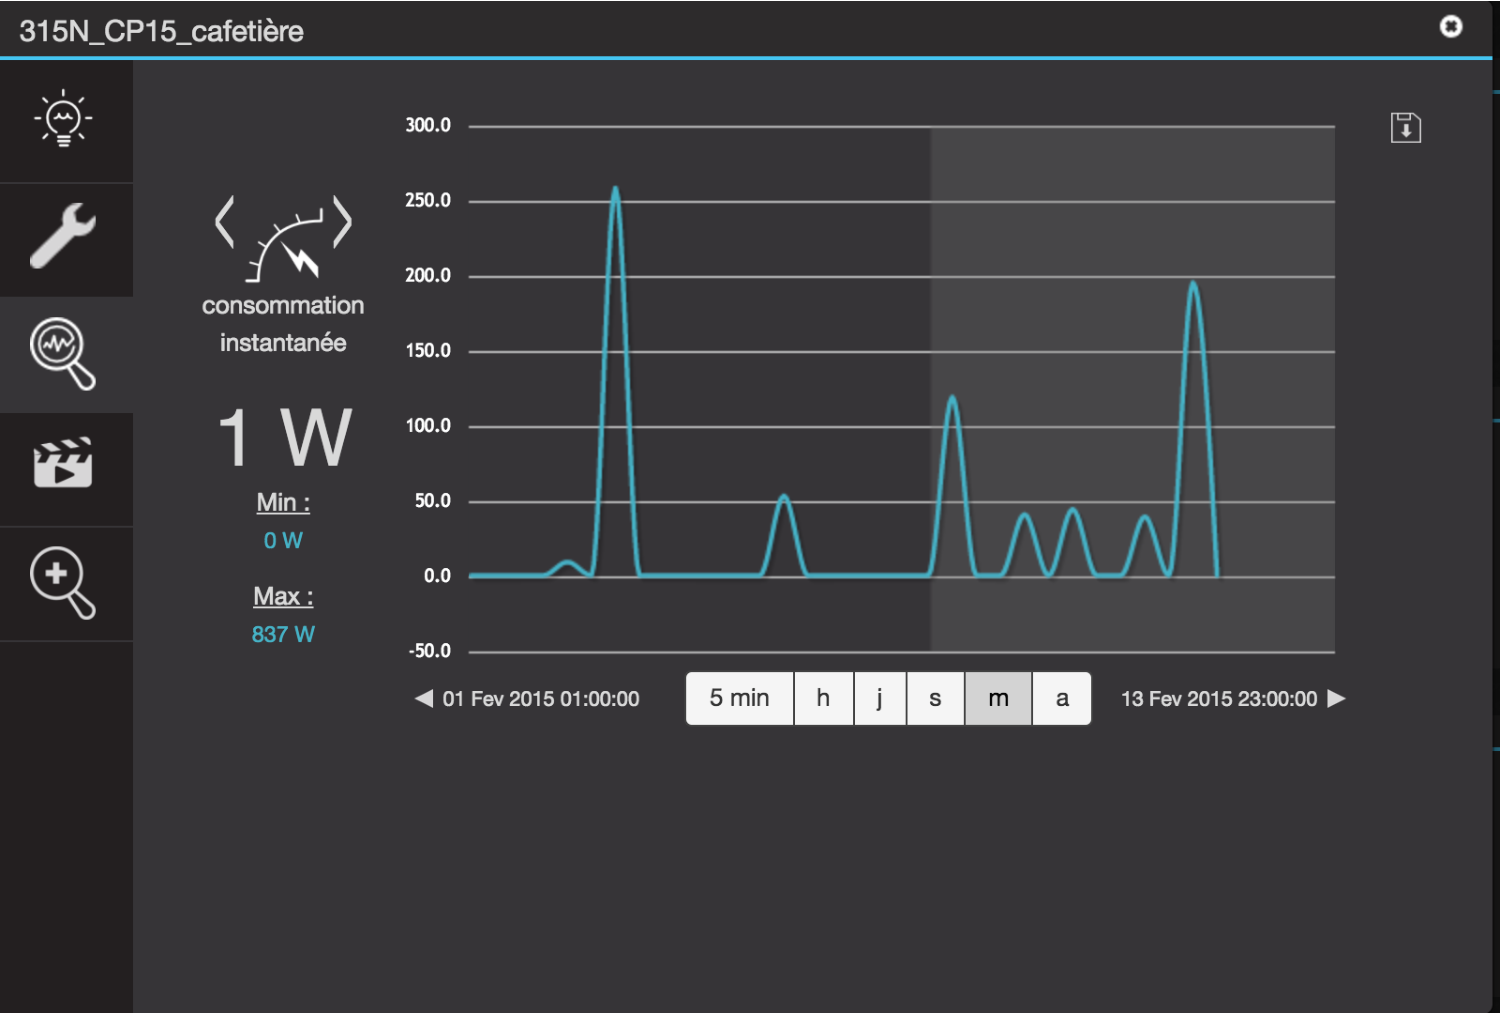
\includegraphics[width=1\textwidth]{./chapters/chapter3/images/A_web3.pdf}
%  \vspace{1.5}
\centerline{(c) Power measurement display}\medskip
\end{minipage}
\caption{Athemium web interface.}
\label{fig:L22}
%
\end{figure}

In this experiment, six devices including fridge, coffee machine, kettle, microwave, television and screen monitor are connected to power meters, as shown in Figure~\ref{fig:L23}. Other loads such as lamps, telephone chargers, Internet modem, outlets, etc., are considered as noise sources. Table~\ref{table:t1} shows the power demand of each device, while an example of their daily power consumption as well as aggregate power is illustrated in Figure~\ref{fig:L3}. Based on these retrieved data, state transition probability of each device can be calculated as presented in Figure~\ref{fig:L1}.

\begin{figure}
\centering
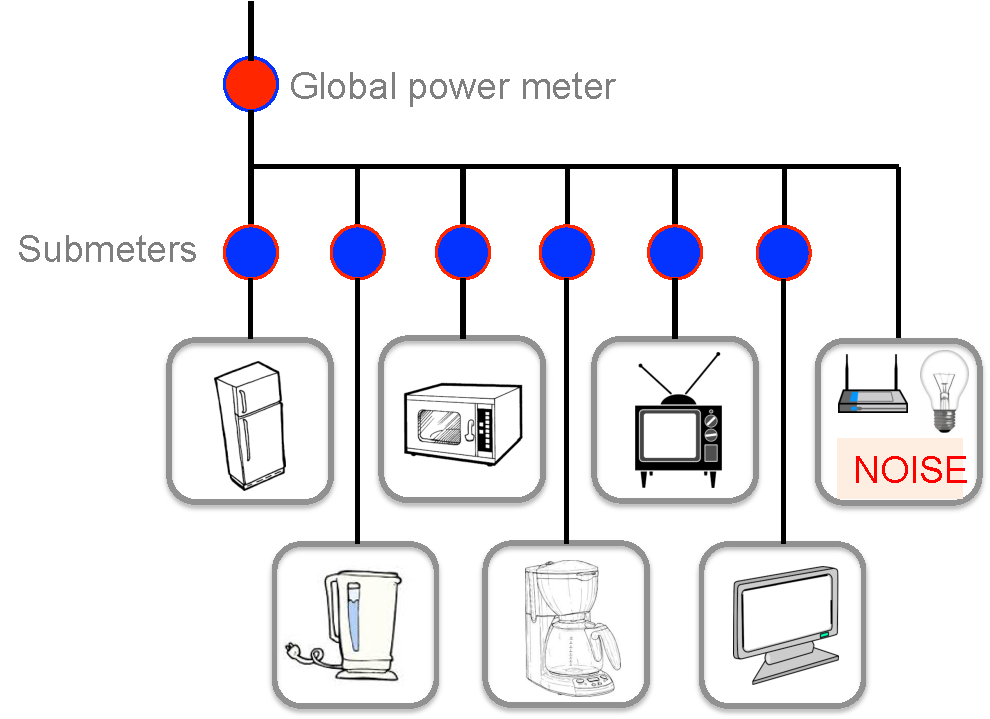
\includegraphics[width=.65\textwidth]{./chapters/chapter3/images/A_topo.pdf} 
\caption{Athemium power measurement: a global power meter measures the aggregate power consumption and some sub-meters provide training data and ground truth data of each device.} 
\label{fig:L23} 
\end{figure}

\begin{table}
\caption{Power demand of devices in Athemium dataset.}\label{table:t1}
\begin{center}
\begin{tabular}{|c|c|c|c|}
\hline
Power demand (Watt)& State 1&State 2&State 3 \\ \hhline{|=|=|=|=|}
Fridge &75& & \\ \hline
Coffee machine &823 &797 & 214 \\ \hline
Kettle & 1667 & 1692 & 1635\\ \hline
Microwave &1350 & 1316 & 1290 \\ \hline
Television & 203 & 29 & \\ \hline 
Screen monitor & 727 & & \\ \hline
\end{tabular}
\end{center}
\end{table}



\begin{figure}
\begin{minipage}[b]{1.0\linewidth}
  \centering
  \centerline{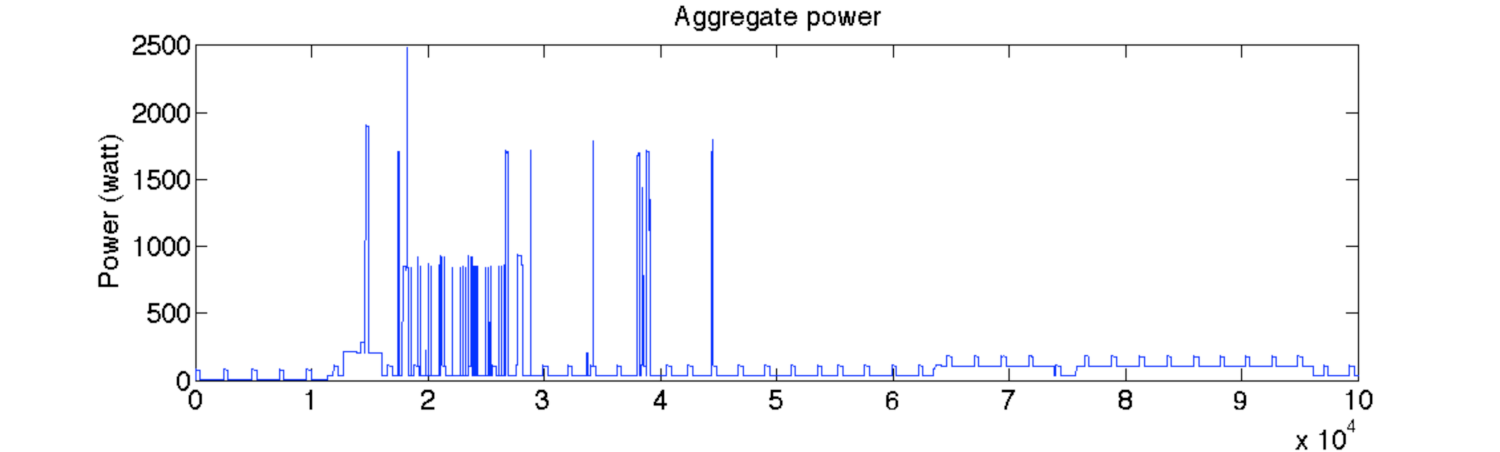
\includegraphics[width=1\textwidth]{./chapters/chapter3/images/A_aggpow.pdf}}
%  \vspace{2.0cm}
  \centerline{(a) Aggregate power consumption}\medskip
\end{minipage}
\begin{minipage}[b]{1.0\linewidth}
  \centering
  \centerline{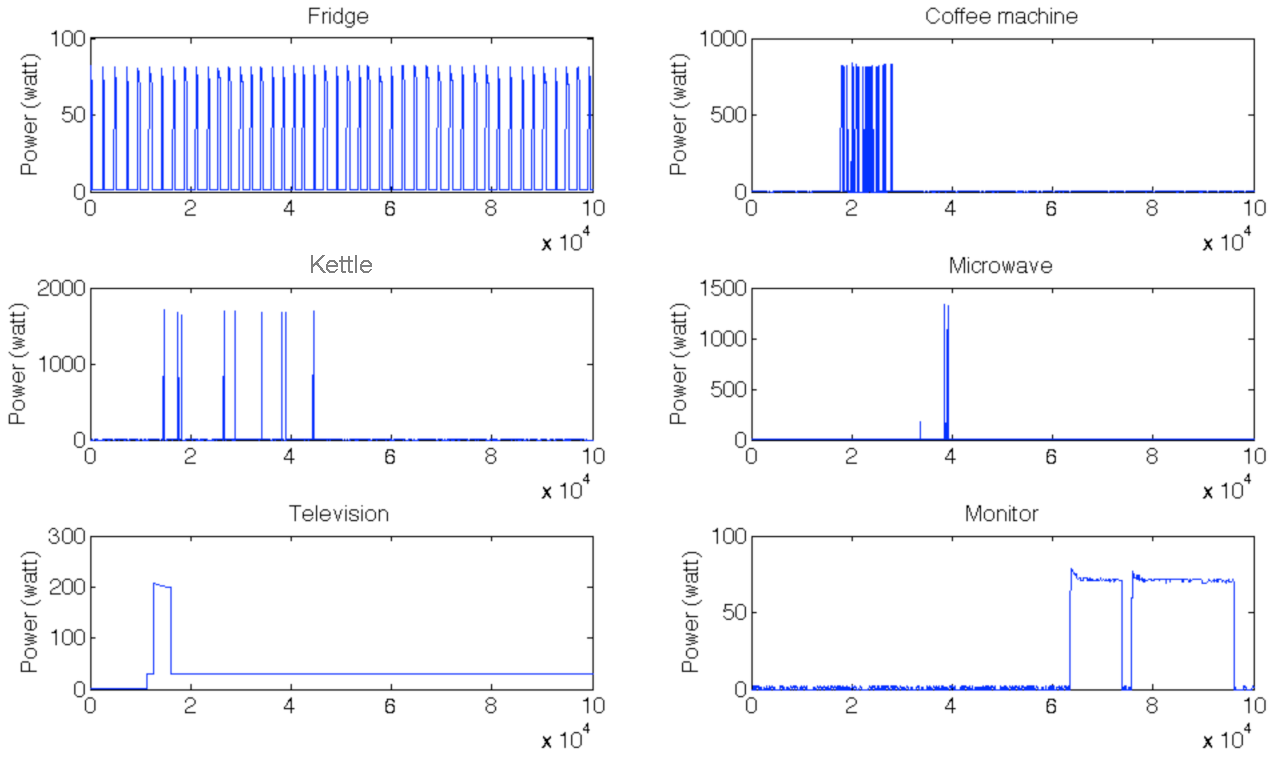
\includegraphics[width=1\textwidth]{./chapters/chapter3/images/A_pow.pdf}}
%  \vspace{2.0cm}
  \centerline{(b) Power consumption of each individual device}\medskip
\end{minipage}
\caption{Power measurement of the devices in Athemium dataset during one day.}
\label{fig:L3} 
\end{figure}




%\subsection{The Average-Case SNR in Chameleon ONoC}\label{resultl1}
To evaluate the algorithms, three metrics are used including \textit{precision} ($pr$), \textit{recall} ($rc$) and \textit{F-measure} ($Fm$)~\cite{Olson2008}, which are theoretically defined as:
\begin{eqnarray}\label{eva-metrics}
pr &=& \frac{TP}{TP+FP},\\
rc &=& \frac{TP}{TP+FN},\\
Fm &=& \frac{2\times pr \times rc}{pr+rc},
\end{eqnarray}
where $TP$, $FP$ and $FN$ are the number of true positives, false positives and false negatives, respectively. A true positive is a true detection of an event, while a false positive (false negative) means a non-event (event) being not correctly detected. As a consequence, the precision can be considered as the reliability of a detected event and the recall is the sensibility to the events of algorithms. Meanwhile, F-measure is interpreted as a weighted average of the precision and recall, which reaches its best value at 1 and worst at 0. For example, if there are 1500 of 2000 time instants that a fridge operates are correctly detected, we have $TP=1500$ and $FN=500$. Similarly, $FP = 200$ if 200 instants that the device is turned off are detected as on. As a consequence, we can obtain:

\begin{eqnarray*}
pr &=& \frac{1500}{1500+200} = 0.88,\\
rc &=& \frac{1500}{1500+500} = 0.75,\\
Fm &=& \frac{2\times 0.88 \times 0.75}{0.88+0.75} = 0.81.
\end{eqnarray*}


\begin{figure}
\centering
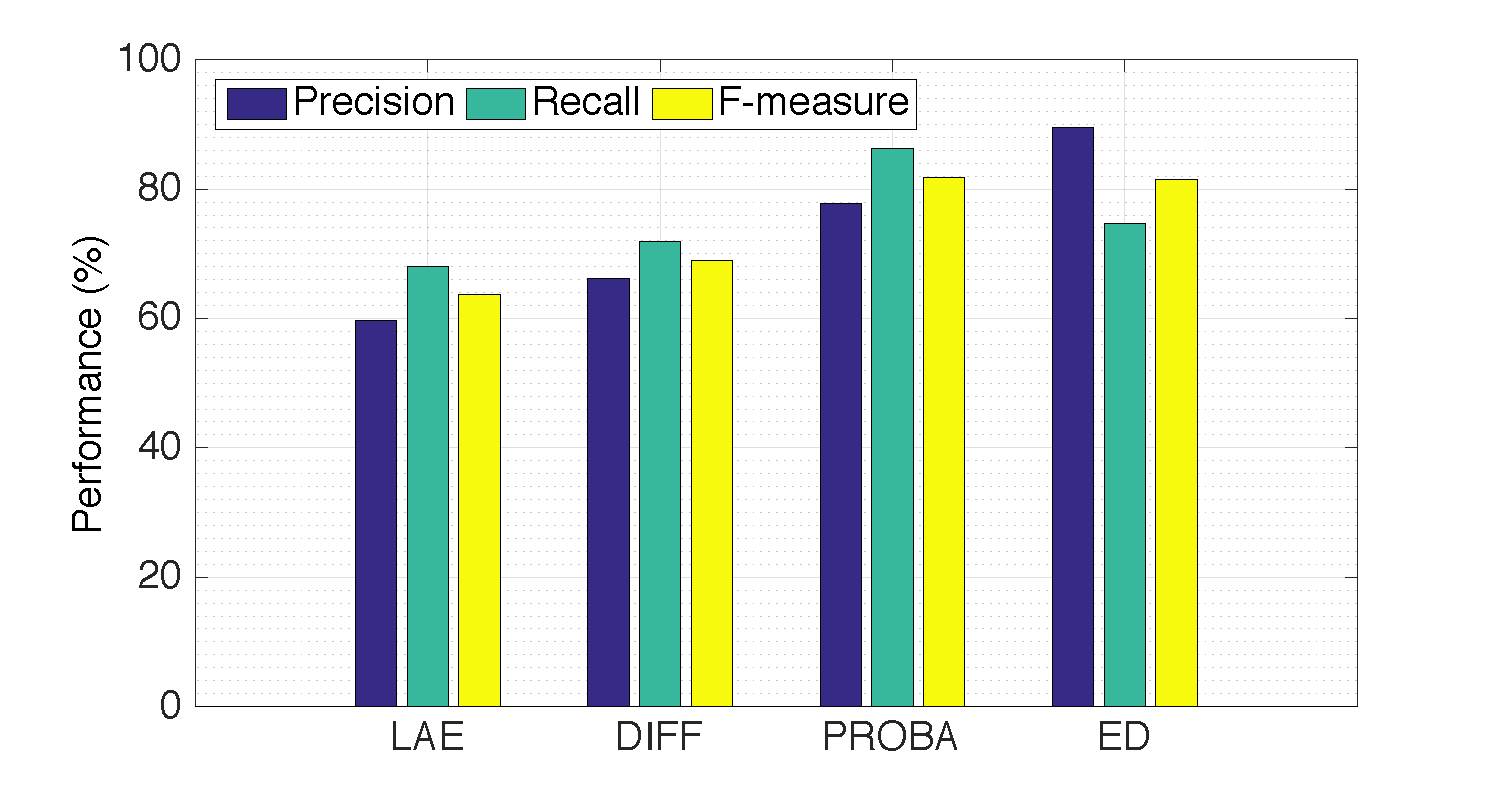
\includegraphics[width=.8\textwidth]{./chapters/chapter3/images/l1_perf.pdf} 
\caption{Performance of the proposed algorithms including LAE, state difference based (DIFF) and transition probability based (PROBA) compared with edge detection algorithm (ED) applied to Athemium data.}
\label{fig:L4} 
\end{figure}
In our Matlab simulation, 30$\%$ of data are used to learn the parameters while state detection algorithms are applied to the remaining.
In Figure~\ref{fig:L4}, performance of the three proposed algorithms with Athemium dataset is shown in comparison with the edge detection algorithm. Apparently, the brute force algorithm without any additional information shows a worse performance than the edge detection approach. While the edge detection algorithm can detect the devices with an overall precision of 89.58$\%$ and recall of 74.65$\%$, the LAE based algorithm only shows a poor performance of 60$\%$ and 69$\%$, respectively. This result comes from the fact that there are some devices consuming a close power level, e.g. coffee machine (214W) and television (203W). Nevertheless, because the coffee machine has three states, the detection based on the edges height is more effective. This is also the reason why considering the state transition of the devices, executed by selecting a subset of suitable combinations giving an error closed to the least value and applying the difference between each combination with the previous state as a criterion to select the solution, can increase the performance of the brute force algorithm. Concretely, the precision can be improved from 60$\%$ to 67$\%$ and the recall from 69$\%$ to 71$\%$. Especially, the performance improvement is more significant if the state transition probability is applied instead of the Hamming distance between the state combinations. Although performing a lower precision (79$\%$ \emph{vs.} 89.58$\%$), the probability based algorithm shows a better recall (87$\%$) than the edge detection one (74.65$\%$), which results in a close F-measure (81.8$\%$ \emph{vs.} 81.43$\%$) for both algorithms.

Table~\ref{table:t2} details the performance of the proposed algorithms correlated to each individual device. Apparently, the LAE based algorithm shows a high reliability in detecting the kettle ($pr=96.89\%$) while it is sensible to the operation of the coffee machine ($rc=99.05\%$) and television ($rc=95.74\%$). The fridge and microwave with many spikes on the power signal are identified with a lower precision than other devices ($pr=43.08\%$ and $pr=44.30\%$, respectively). Meanwhile, the state difference based algorithm allows to significantly improve the performance of the television (F-measure from 86.12$\%$ to 91.02$\%$) and kettle (60.53$\%$ to 76.9$\%$). With the transition probability based algorithm, the remarkable increase of the performance corresponds to the fridge (56.22$\%$ to 75.30$\%$), kettle (60.53$\%$ to 84.43$\%$), microwave (56.03$\%$ to 67.53$\%$) and monitor (55.25$\%$ to 79.13$\%$).

\begin{table}
\caption{Detailed performance of the three proposed algorithms including LAE based, state difference based (DIFF) and state transition probability based (PROBA) to detect each device: fridge (FR), coffee machine (CF), kettle (TE), microwave (MW), television (TV) and monitor (MO).}\label{table:t2}
\begin{center}
\begin{tabular}{|c|c|c|c|c|c|c|c|c|c|}
\hline
&\multicolumn{3}{|c|}{Precision ($\%$)} & \multicolumn{3}{|c|}{Recall ($\%$)}&\multicolumn{3}{|c|}{F-measure ($\%$)}\\
\hline
&LAE & DIFF & PROBA & LAE & DIFF & PROBA & LAE & DIFF & PROBA\\
\hline
FR & 43.08 &44.24&63.80&80.88&73.95&91.86&56.22&55.36&75.30\\
\hline
CM&76.64&80.25&76.34&99.05&98.94&98.90&86.42&86.62&86.17\\
\hline
TE &96.89&98.97&98.98&44.01&62.88&73.61&60.53&76.90&84.43\\
\hline
MW & 44.30 & 47.01&57.63&76.22&81.55&81.55&56.03&59.64&67.53\\
\hline
TV &78.25&86.99&83.05&95.74&95.44&95.79&86.12&91.02&89.97\\
\hline
MO & 55.52&57.80&89.83 &54.99&59.86&70.71&55.25&56.67&79.13\\
\hline
\end{tabular}
\end{center}
\end{table}

As mentioned in the previous section, an important parameter affecting the performance of the state difference based and state transition probability based algorithms for $l1$-norm minimization problem is the threshold $\gamma$ to select the retained combinations. If this threshold is too small, the true combination may be left out. In contrast, if it is too high, too many combinations are maintained and that may cause the decrease of the performance as well as the increase of the execution time. Figure~\ref{fig:L6} shows the effect of the threshold $\gamma$ on the performance of the algorithm based on the state transition probability with the best result obtainable at $\gamma = 3$.

\begin{figure}
\centering
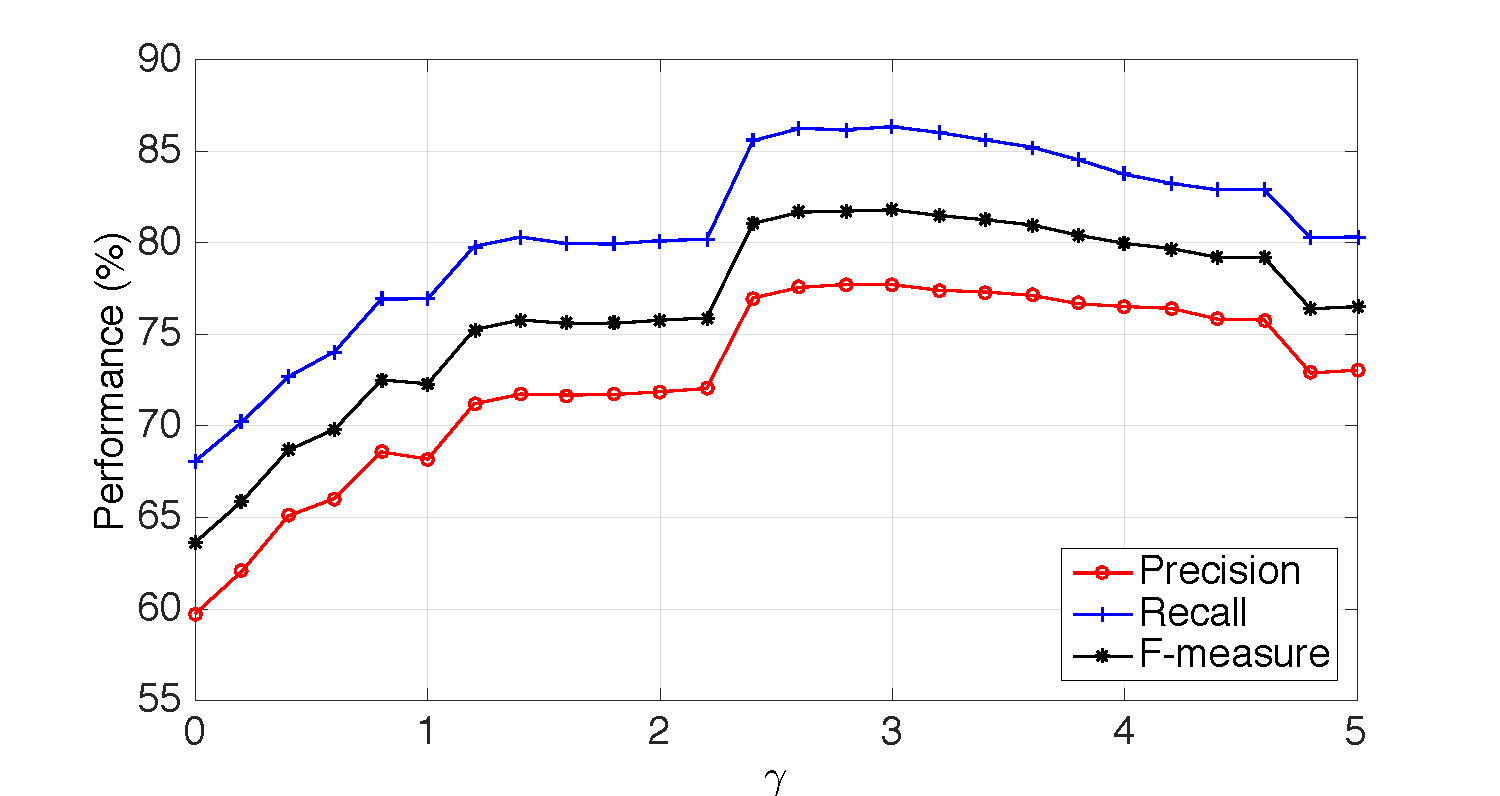
\includegraphics[width=.8\textwidth]{./chapters/chapter3/images/PROBAvsTHR.pdf} 
\caption{Effect of threshold $\gamma$ on the performance of state transition probability based algorithm simulated with Athemium dataset.}
\label{fig:L6} 
\end{figure}

Although the additional subroutines significantly improve the performance of LAE based algorithm with Athemium data, it is still less effective when applied to other dataset with more confusions among combinations as well as too much \emph{ghost power} consumed by unmonitored devices such as REDD \emph{House 1}~\cite{Kolter11redd}, as illustrated in Figure~\ref{fig:L7}. In this dataset, besides the devices connected to an individual power meter, the total power consumption of other unmonitored devices can be considered as consumed by a unique unknown device. Though there are over 20 channels, we use only nine channels as shown in Table~\ref{table:t3}, because the others have no activation of devices. Besides, two main phases of electricity are combined to have a unique main power signal.
As shown in Figure~\ref{fig:L7}, the precision of $l1$-norm minimization based algorithm can be improved from 58.63$\%$ to 60.75$\%$ and the recall from 64.62$\%$ to 70.43$\%$ with state transition probability. Nevertheless, they are still lower than the performance given by the edge detection one, with $pr=80.95\%$ and $rc = 70.58\%$, respectively. Therefore, in the next chapter, a new monitoring system will be used to significantly improve the performance of NILM algorithms based on probability information of each device provided by an additional sensor network.

\begin{table}
\caption{Power demand of devices in REDD dataset \emph{House 1}.}\label{table:t3}
\begin{center}
\begin{tabular}{|c|c|c|c|}
\hline
Power demand (watt)& State 1&State 2&State 3 \\ \hhline{|=|=|=|=|}
Oven&4140&4075&3377 \\ \hline
Fridge &193&423 & \\ \hline
Dish washer & 214& 1107 & \\ \hline
Lighting & 169 & 275 & 345 \\ \hline
Microwave &1531 & 1571 & 1396 \\ \hline
gfi bathroom & 1595 & & \\ \hline
Outlet & 1056 & & \\ \hline
Outlet & 1521 & & \\ \hline
Washer dryer & 5097 & 5250 & 5008 \\ \hline
\end{tabular}
\end{center}
\end{table}

\begin{figure}
\centering
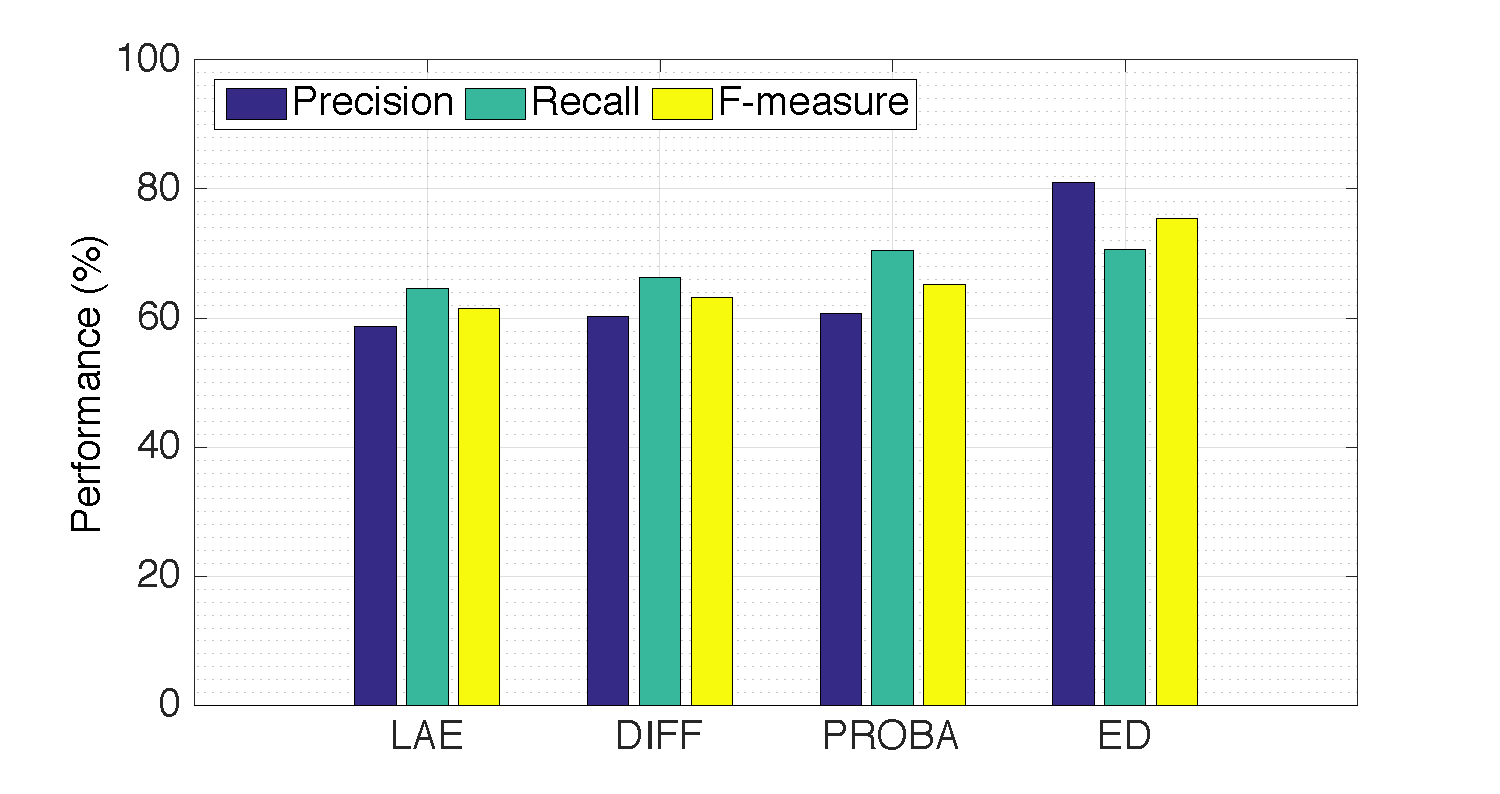
\includegraphics[width=.8\textwidth]{./chapters/chapter3/images/R1_l1_perf.pdf} 
\caption{Performance of the proposed algorithms including LAE, state difference based (DIFF) and transition probability based (PROBA) compared with the edge detection (ED) algorithm applied to REDD \emph{House 1}.}
\label{fig:L7} 
\end{figure}


\section{Conclusions}
In this chapter, we directly solve the $l1$-norm minimization problem in NILM by applying three proposed algorithms, including:
\begin{itemize}
\item LAE-based algorithm: this algorithm is a brute force method to apply all possible combinations of states to calculate the absolute error between the aggregate power and the total power demand corresponding to each combination. The combination giving the least value of error is selected to determine the state of devices;
\item State difference based algorithm: instead of selecting the least absolute error, this algorithm finds all possible combinations giving an error around it and then compares with the previous state to to select one having the smallest Hamming distance;
\item State transition probability based algorithm: the solution is selected among suitable combinations by considering the state transition probability from the previous state to the current state of each device.
\end{itemize}

The experimental results show that by applying the state difference and state transition probability to select suitable combination of state, performance of the brute force algorithm is improved and outperforms the edge detection one. Nevertheless, these proposed algorithms show an exponential complexity and may be intractable with larger number of devices. In addition, an excessive training data is necessary to learn the characteristics of each device such as power demand and state transition probability.
% Chapter 4

% NOTE: 1. REPLACE THE MODEL AND DP BY SENSYS PAPER, RESIMULATE THE RESULTS FOR CPH AND ADD THE RESULT OF DP 

\chapter{Error Correction Codes in optical interconnects -- Energy efficiency channel} % Write in your own chapter title
\label{SmartSense}
%\addtotoc{State of the Arts}
\lhead{\emph{SmartSense: Sensor-Aided NILM}} % Write in your own chapter title to set the page header

\section{The transmitted laser power and communication loss modeling}\label{model}
\subsection{Point-to-point optical interconnect}
In NILM, the disaggregation algorithms always try to extract the features from the overall electrical load signal to identify the devices. However, how can we discern the devices with the same power characteristics? For example~\cite{Laughman03PEM}, if the algorithms use the features related to the average power consumption such as power level, length of steady state, step-change, etc., to discriminate the devices, it can lead to a false detection when  separating an incandescent light bulb and a desktop computer, which consume the same power of 150W.
\subsection{Model of loss}

%---------------------------------
\begin{figure}[!hbt]
\begin{center}
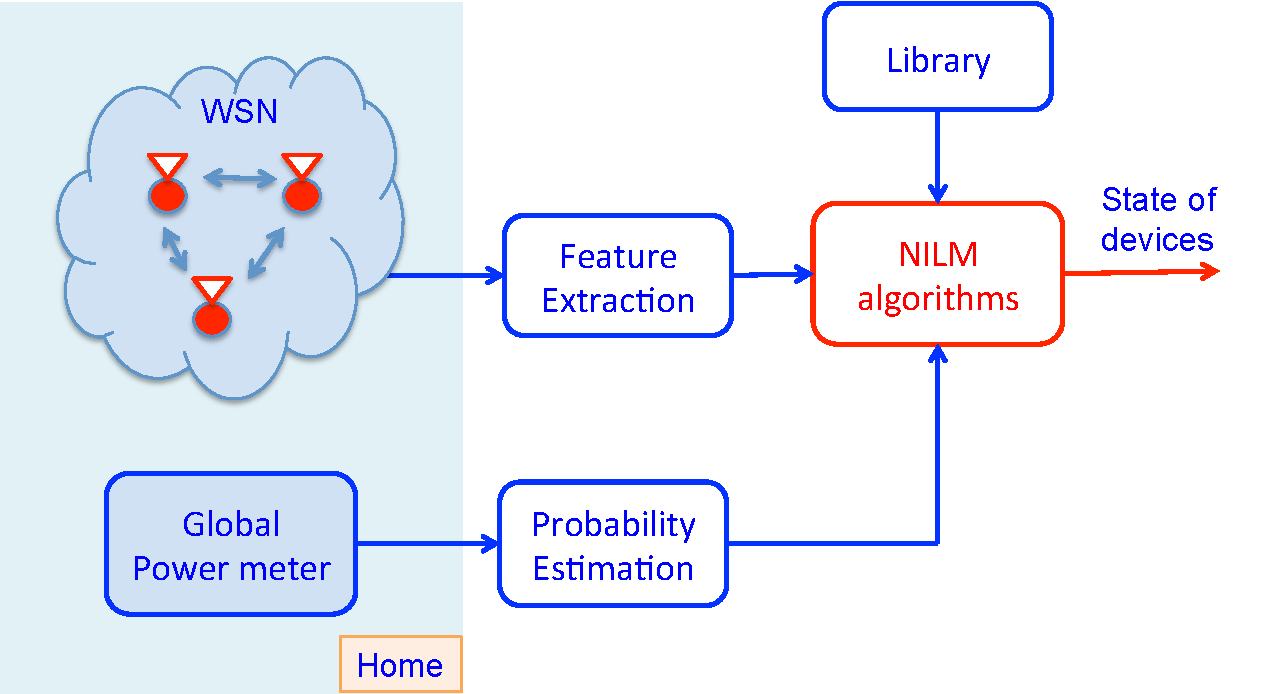
\includegraphics[width=1\textwidth]{./chapters/chapter4/images/SSmodel.pdf}
\caption{SmartSense system model: an NILM system combining with a sensor network providing the operating probability of some specific devices.}
\label{fig:S1}
\end{center}
\end{figure}

To overcome this restriction and improve the performance of the detection algorithms, we propose to use the operating probability of each device as an additional feature. A low-cost and low-power WSN is proposed to be deployed in homes and buildings to monitor the operation of some specific devices. A system combining NILM with such a WSN, called SmartSense, is shown in Figure~\ref{fig:S1}. However, different from ViridiScope~\cite{Kim09Ubicomp} which is fully intrusive, our approach only monitors a subset of all devices, which makes it less intrusive. On the other hand, the purpose of the WSN is not to directly provide the state of devices but to estimate their state probability to improve the performance of NILM algorithms. Depending on the type of monitored devices, the corresponding sensors are deployed.
For example, the operation of light-emitting devices such as screens, televisions, lamps can be detected by using the light intensity sensors, while the motor-based devices such as washing machine, fridge can be identified with a vibration sensor. Besides, other types of sensors can also be used to monitor other electrical equipment such as microphones, magnetometers, etc. A local algorithm in the WSN is then constructed to transform the detection of sensors to the probability of the corresponding devices. The probability estimation is executed based on the performance evaluation metrics including \textit{precision} and \textit{negative predictive value}, calculated by
\begin{eqnarray}
pr &=& \frac{TP}{TP+FP}\\
npv &= &\frac{TN}{TN+FN},
\end{eqnarray}
where $pr$, $TP$, $FP$ and $FN$ are defined in Chapter~\ref{l1norm} on page~\pageref{eva-metrics}, while $npv$ and $TN$ denote the negative predictive value and the number of true negatives, respectively. A true negative is defined as a true detection of non-event. Therefore, the negative predictive value can be considered as the reliability of a detected non-event.
As a consequence, when a device is determined as running, the probability of on-state and off-state are equal to $pr$ and $(1-pr)$, respectively. In contrast, when not running, they correspond to $(1-npv)$ and $npv$. For other unmonitored devices, all states can occur with the same probability.
\subsection{BER and Laser Power Trade-Offs for uncoded optical interconnect}
To prove the efficiency of the operating probability in improving the performance of NILM, in this research, we propose two main approaches for the state detection. In the first approach, the minimization problem \eqref{eqL1} of NILM can be modeled as a Knapsack problem and solved by two proposed algorithms including Compositional Pareto-algebraic Heuristic (CPH) and Dynamic Programming (DP). Meanwhile, the second one applies the probability to two existing algorithms including edge detection~\cite{Hart92} and dynamic time warping~\cite{Liao14}. In the rest of this chapter, the word \textit{event} is used to denote an on-state in the CPH, DP and DTW algorithms and an edge in the ED one.






\section{Error Correction Codes for optical interconnects}\label{knapsack}
%%------------------ modification: add a part of one-state devices
Let consider again the $l1$-norm minimization problem \eqref{eqL1} of NILM:
\begin{eqnarray}\label{eqSS2}
& &\min_{\mathbf{s}}{E(\mathbf{s}) = \left|\sum_{i=1}^N{\sum_{j=1}^{m_i}{w_{ij}s_{ij}}}-x\right|} \\
\mbox{subject to}&&s_{ij}\in \{0,1\},  i=1,\ldots,N,j=1,\ldots,m_i \nonumber\\
& & \sum_{j=1}^{m_i}{s_{ij}}\in \{0,1\}, i=1,\ldots,N, \nonumber
\end{eqnarray}
where $E(\mathbf{s})$ can be interpreted as the absolute error between the measured aggregate power consumption and the total power demand of all operating devices. Solving Eq.~\eqref{eqSS2} is equivalent to find a vector $\mathbf{s}$ comprising all state indicators $s_{ij}$, $i=1,\ldots,N, j=1,\ldots,m_i$ of all devices, i.e., $\mathbf{s}=\{s_{11},\ldots,s_{1m_1},s_{21},\ldots,s_{2m_2},\ldots,s_{N1},\ldots,s_{Nm_N}\}$.
In Chapter \ref{l1norm}, this problem is solved by applying three proposed methods including least absolute error, state difference and state transition probability. However, in the SmartSense system, by using an additional parameter related to the operating probability, a new problem is formulated from \eqref{eqSS2} and two methods are proposed to solve it including CPH and DP. The on/off state probability of each device is estimated as mentioned in Section \ref{model}. Nevertheless, as the sensors can only detect if a device is on or off but cannot distinguish its different power states, the operating probability will then be equally divided to all states, i.e. $p_{ij} = p_i/m_i,j=1,\ldots,m_i$. Let consider the problem formulation in the case that each device has only two states, on or off, and in a general case in which each device has a finish number of power states.


\subsection{Problem formulation}
%%------------------ modification: add a part of one-state devices

\paragraph*{One-state devices}
Firstly, let consider the simplest case in which each device can only operate at a unique stable state with a corresponding power demand $w_i$. Denote $s_i$ as the state indicator of device $i$ and notation $^{(1)}$ for one-state using case, problem \eqref{eqSS2} becomes:
\begin{eqnarray}\label{eqSS3}
& &\min_{\mathbf{s}}{E^1(\mathbf{s})=\left |\sum_{i=1}^N{w_is_i}-x\right |}\\
\mbox{subject to } & &s_i\in \{0,1\}, i=1,\ldots ,N, \nonumber
\end{eqnarray}
where $\mathbf{s} = \{s_1,s_2,\ldots ,s_N\}$.
Assuming device $i$ is in on-state with probability of $p_i,0\leq p_i\leq 1$, the probability mass function is then:
\begin{equation}\label{eqSS4}
Pr(s_i) = p_i^{s_i}(1-p_i)^{(1-s_i)}.
\end{equation}
%
Because the operation of $N$ devices is assumed to be independent, the coincidence probability, the probability that all events happen simultaneously, is as follows:
\begin{eqnarray}\label{eqSS6}
Pr(\mathbf{s})& =& \prod_{i=1}^N{Pr(s_i)}\nonumber \\
&=&\prod_{i=1}^N{p_i^{s_i}(1-p_i)^{(1-s_i)}}.
\end{eqnarray}
To reduce the computational complexity, the log-linear form can be applied to transform the multiplication in~\eqref{eqSS6} to an addition, which gives:
\begin{eqnarray}\label{eqSS7}
L^1(\mathbf{s}) &=& -\log{(Pr\left(\mathbf{s})\right)} \nonumber \\
&=&-\log{\left( \prod_{i=1}^N{p_i^{s_i}(1-p_i)^{(1-s_i)}}\right)}\nonumber \\
&=& -\sum_{i=1}^N{\left(s_i\log{p_i}+(1-s_i)\log{(1-p_i)}\right)}.
\end{eqnarray}
Denote $L^1(s_i) = (1-s_i) l^1_{i0}+s_i l^1_{i1}$ with $l^1_{i0} = -\log{(1-p_i)}$ and $l^1_{i1} = -\log{p_i}$, Eq.~\eqref{eqSS7} can be written as
\begin{eqnarray}
L^1(\mathbf{s}) &=& \sum_{i=1}^N{L^1(s_i)}.
\end{eqnarray}
By this transformation, the increase of $Pr(\mathbf{s})$ corresponds to the decrease of $L^1(\mathbf{s})$. The problem is now to find a combination of operating devices not only giving the least absolute error $E^1(\mathbf{s})$ but also having the maximum probability, i.e. the minimum value of $L^1(\mathbf{s})$. Therefore, the problem~\eqref{eqSS3} is developed to a co-optimization problem as follows:
\begin{eqnarray}\label{eqSS8}
& &\min_{\mathbf{s}}{\left[P^1(\mathbf{s}) = E^1(\mathbf{s}) + \lambda \times L^1(\mathbf{s})\right]}\\
\mbox{subject to } & & \sum_{i=1}^N{w_is_i} \leq x+\epsilon \nonumber \\
& &s_i\in \{0,1\}, i=1,\ldots ,N, \nonumber
\end{eqnarray}
where $\lambda$ is a regularization parameter and empirically chosen, $\epsilon$ corresponds to the standard deviation of the aggregate power consumption. The problem~\eqref{eqSS8} is a kind of \textbf{0-1 Knapsack problem}, in which the aim is to fill the knapsack by selecting among various objects, each of which having a particular weight and giving a particular profit~\cite{Lagoudakis96the0-1}. The optimization problem is then to choose the objects in order to obtain the maximum profit while respecting the knapsack capacity.
%%------------------ end modification




%=======================================
\paragraph*{Multi-state devices}
Return to the general case where each device has a finite number of states, the following condition needs to be satisfied:
\begin{equation}
\sum_{j=1}^{m_i}{s_{ij}}\leq 1,s_{ij} \in \{0,1\}, i=1,\ldots,N,
\end{equation}
where $m_i$ is the number of states of device $i$.
Therefore, the operating probability of device $i$, denoted as $Pr(\mathbf{s}_i)$, $\mathbf{s}_i = \{s_{i1},s_{i2},\ldots,s_{im_i}\}$, is
\begin{eqnarray}\label{eqSS9}
Pr(\mathbf{s}_i) = p_{i0}^{\prod_{j=1}^{m_i}{(1-s_{ij})}}\times \prod_{k=1}^{m_i}{p_{ik}^{\prod_{j=1,j\neq k}^{m_i}{s_{ik}(1-s_{ij})}}},
\end{eqnarray}
where  $p_{i0} = p(s_{ij}=0, j=1,\ldots,m_i)$ is the probability of off-state of device $i$ and $p_{ik} = p(s_{ik}=1,s_{ij}=0,\forall j\neq k)$ is the probability of operating at state $k$. Intuitively, we have $\sum_{j=0}^{m_i}{p_{ij}}=1$. 
Transforming Eq.~\eqref{eqSS9} to log-linear form gives
\begin{eqnarray}\label{eqSS10}
L^M(\mathbf{s}_i) &=& -\log{Pr(\mathbf{s}_i)} \nonumber\\
&=& -\prod_{j=1}^{m_i}{(1-s_{ij})}\log{p_{i0}} \nonumber \\
&& - \sum_{k=1}^{m_i}{\left\{\prod_{j=1,j\neq k}^{m_i}{s_{ik}(1-s_{ij})}\log{p_{ik}}\right\}}.
%&=& \sum_{j=0}^{m_i}{l_{ij}}.
\end{eqnarray}
Denoting $l^M_{ik} = -\log{p_{ik}}, k=0,\ldots,m_i$, Eq.~\eqref{eqSS10} can be rewritten as
\begin{equation}
L^M(\mathbf{s}_i) = \prod_{j=1}^{m_i}{(1-s_{ij})l^M_{i0}}+\sum_{k=1}^{m_i}{\left\{\prod_{j=1,j\neq k}^{m_i}{s_{ik}(1-s_{ij})}l^M_{ik}\right\}}.
\end{equation}
Similarly to the case of one-state devices, the concincidence probability $Pr(\mathbf{s})$, $\mathbf{s} = \{\mathbf{s}_1,\ldots,\mathbf{s}_N\}$, and its respective log-linear form $L^M(\mathbf{s})$ can be formulated as
\begin{eqnarray}\label{eqSS11}
Pr(\mathbf{s}) &=& \prod_{i=1}^N{Pr(\mathbf{s}_i)}\\
L^M(\mathbf{s})& =& \sum_{i=1}^N{L^M(\mathbf{s}_i)}.
\end{eqnarray}

As a consequence, the co-optimization problem to minimize the least absolute error in problem~\eqref{eqSS2} and maximize the coincidence probability in Eq.~\eqref{eqSS11} is modified to
\begin{eqnarray}\label{eqSS12}
&&\min_{\mathbf{s}}{\left[P^M(\mathbf{s}) = E^M(\mathbf{s}) + \lambda \times L^M(\mathbf{s})\right]} \\
\mbox{subject to } &&\sum_{i=1}^N{\sum_{j=1}^{m_i}{w_{ij}s_{ij}}}\leq x+\epsilon \nonumber\\
&& \sum_{j=1}^{m_i}{s_{ij}} \leq 1, j=1,\ldots,N \nonumber\\
&&s_{ij}\in \{0,1\},  i=1,\ldots ,N,j=1,\ldots,m_i.\nonumber
\end{eqnarray}
Considering the state of devices as objects and the aggregate power consumption as the knapsack capacity, Eq.~\eqref{eqSS11} is equivalent to the Knapsack problem. The state detection is apparently similar to dividing the available objects into groups and selecting a maximum of one object from each group to fill the knapsack. Hence, the problem~\eqref{eqSS12} can be considered as a so-called \textbf{Multiple-Choice Knapsack (MCK)} problem~\cite{Bean88}.

In SmartSense, at each data point, an algorithm will be applied to solve the co-optimization problem to find the corresponding state of each device. To solve the Knapsack problem, the naive and straightforward approach is brute force, as introduced in Chapter~\ref{l1norm}. However, the exponential complexity makes it intractable with large number of devices. Besides, there are several other approaches such as branch and bound \cite{Martello1980276,DYER1984231,Lukata1997}, genetic algorithm \cite{Anagun2006,Singh07,Fukunaga08,Shen11}, dynamic programming (DP)~\cite{Toth79,Bean88}, compositional Pareto-algebraic heuristic (CPH) \cite{Shojaei13,Shojaei5227146,Geilen07,Geilen05,Geilen07acm,Hifi04,Yukish2004}, or combining DP with branch and bound~\cite{Martello99}.

In this study, we focus on CPH and DP, two most effective approaches in Knapsack problem, to apply in the context of SmartSense. These algorithms have some driving parameters allowing to reduce the computational complexity.


\subsection{Error Correction Code implementations -- Case study}\label{sec:algo}
\subsubsection{Extended Hamming codes }\label{CPH}
%---------------------------------

The CPH algorithm is based on a recursive relation  and illustrated by an example in Figure~\ref{fig:SS2}. Figure~\ref{fig:SS2}(a) presents a set of three devices with different operation states. Each state consumes a stable power with a corresponding probability. Assuming at time instant $t$, the aggregate power consumption $x$ is equal to 150~W. With the standard deviation $\epsilon$ of 5~W, the total power demand of any set of operating devices cannot exceed the bound $R=x +\epsilon = 155$~W. Figure~\ref{fig:SS2}(b) shows how the CPH algorithm operates. In the first step, each device is represented as a set of \textit{tuples}, each corresponding to a state. For example, device $D_1$ comprises three tuples: $(0, 23.03,173.03)$, $(50,2.23,102.23)$, $(150,23.03,23.03)$. The first element $d_1$ of each tuple represents the power demand, the second one $d_2$ contains the product of the operating probability in log-linear form and the regularization parameter $\lambda$, equal to 10 in this example, and the third one $d_3$ is calculated from two first elements $d_1$ and $d_2$ as follows:
\begin{eqnarray}
d_1 &=& w\\
d_2 &=& -\lambda \times \log{p}\\
d_3 &=& \left|x-d_1\right|+d_2. \label{eqCPH1}
\end{eqnarray}
\begin{figure}[h]
%\centering
\begin{minipage}[b]{1\linewidth}
  \centering
  \centerline{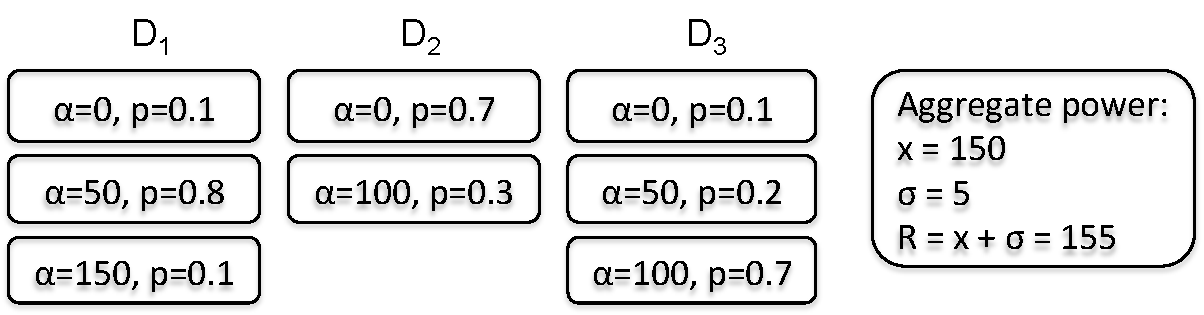
\includegraphics[width=0.8\textwidth]{./chapters/chapter4/images/cph1}}
%  \vspace{2.0cm}
  \centerline{(a)}\medskip
\end{minipage}
\begin{minipage}[b]{1\linewidth}
  \centering
  \centerline{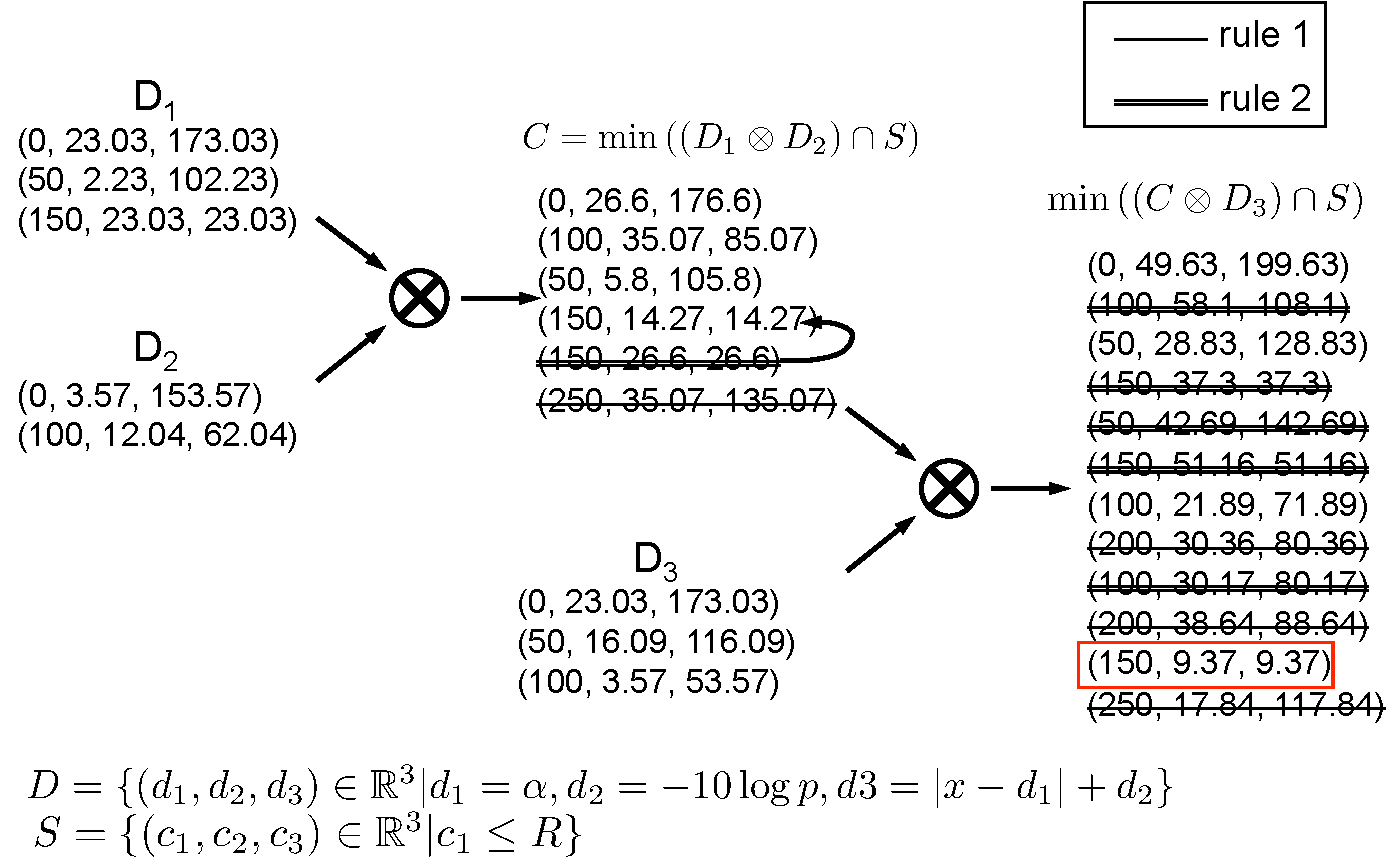
\includegraphics[width=0.9\textwidth]{./chapters/chapter4/images/cph2}}
%  \vspace{2.0cm}
  \centerline{(b)}\medskip
\end{minipage}
%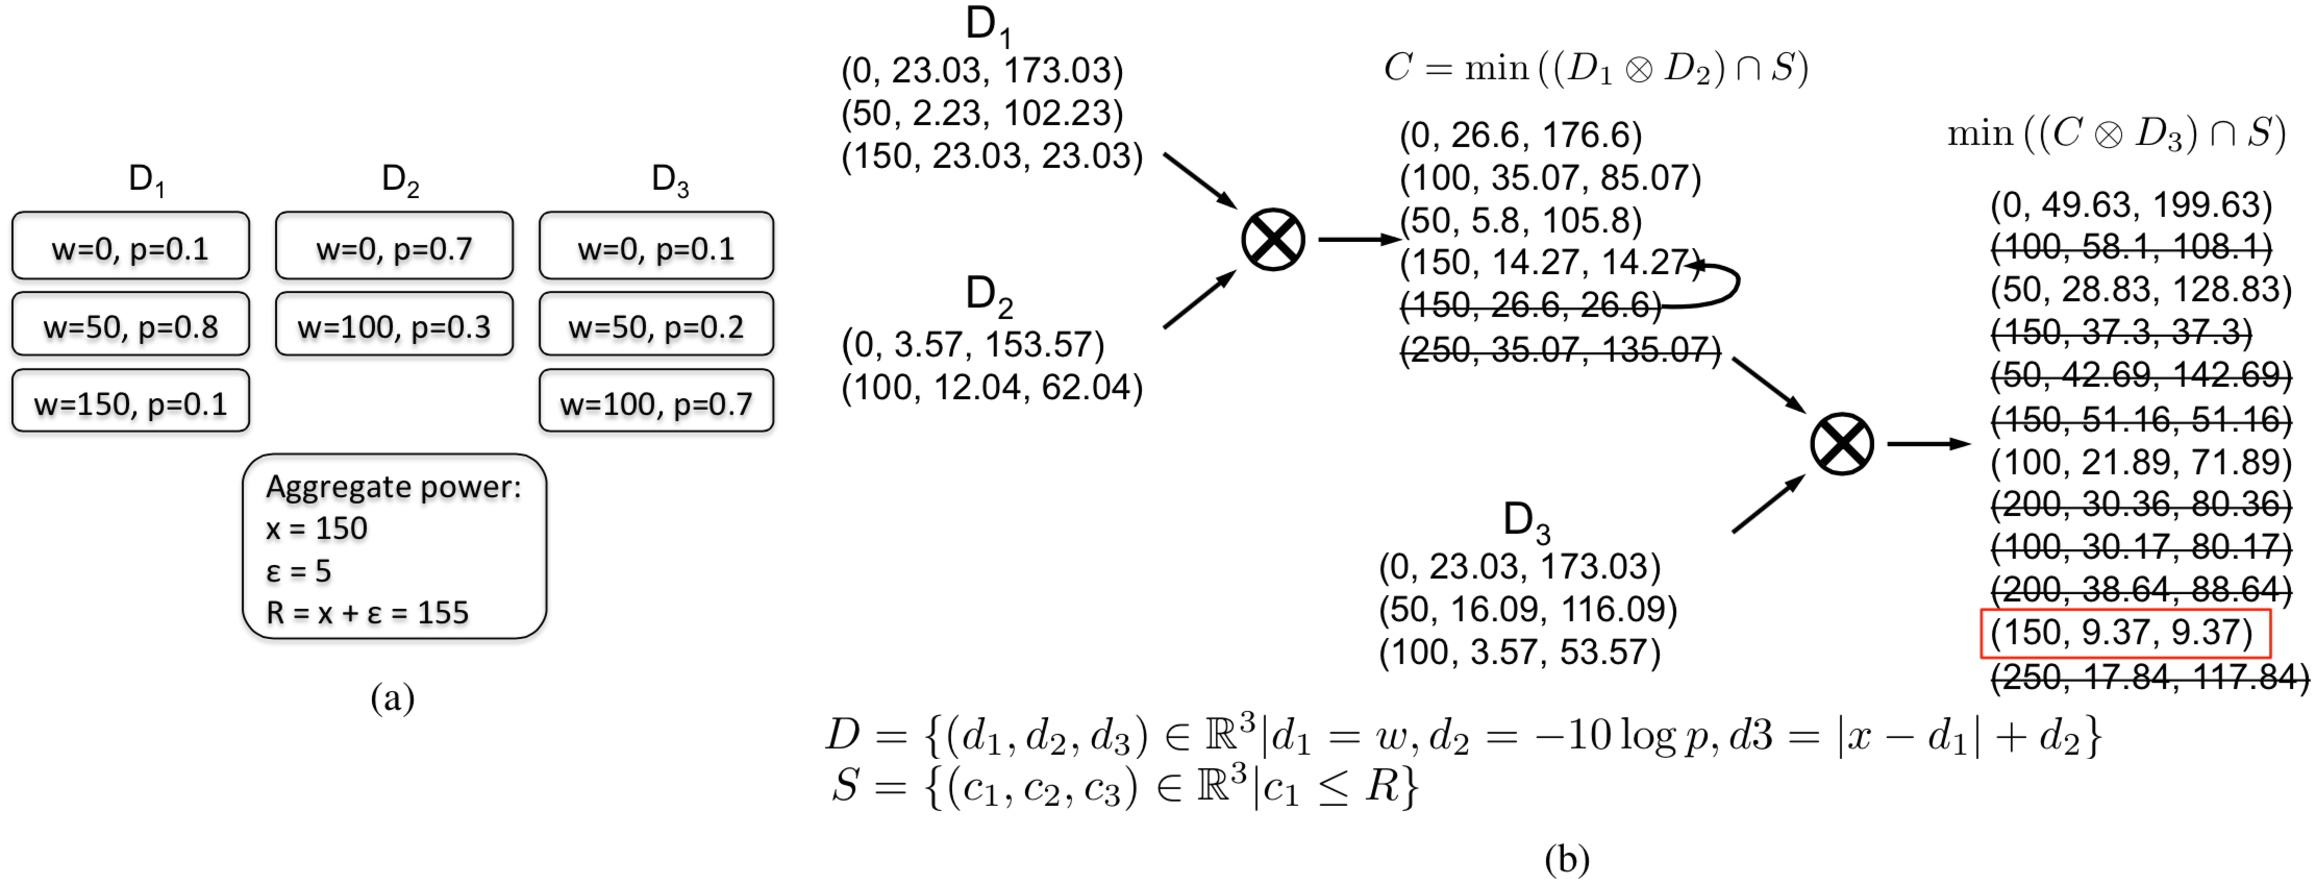
\includegraphics[width=1\textwidth]{./chapters/chapter4/images/CPHex.pdf} 
\caption{Running example of CPH. (a)~Three devices with corresponding power demand and probability of each state as well as the aggregate power consumption. (b)~Each device is represented as a set of tuples, each tuple corresponds to a state. At each iteration, a partial solution can be discarded if its first element (power consumption) exceeds the bound $R$ (rule~1), or its third element is greater than another solution while consuming larger or same power (rule~2). After all sets are combined, the tuple giving the smallest value of the third element is selected as the final solution.} 
\label{fig:SS2} 
\end{figure}

\begin{figure}[ht]
\centering
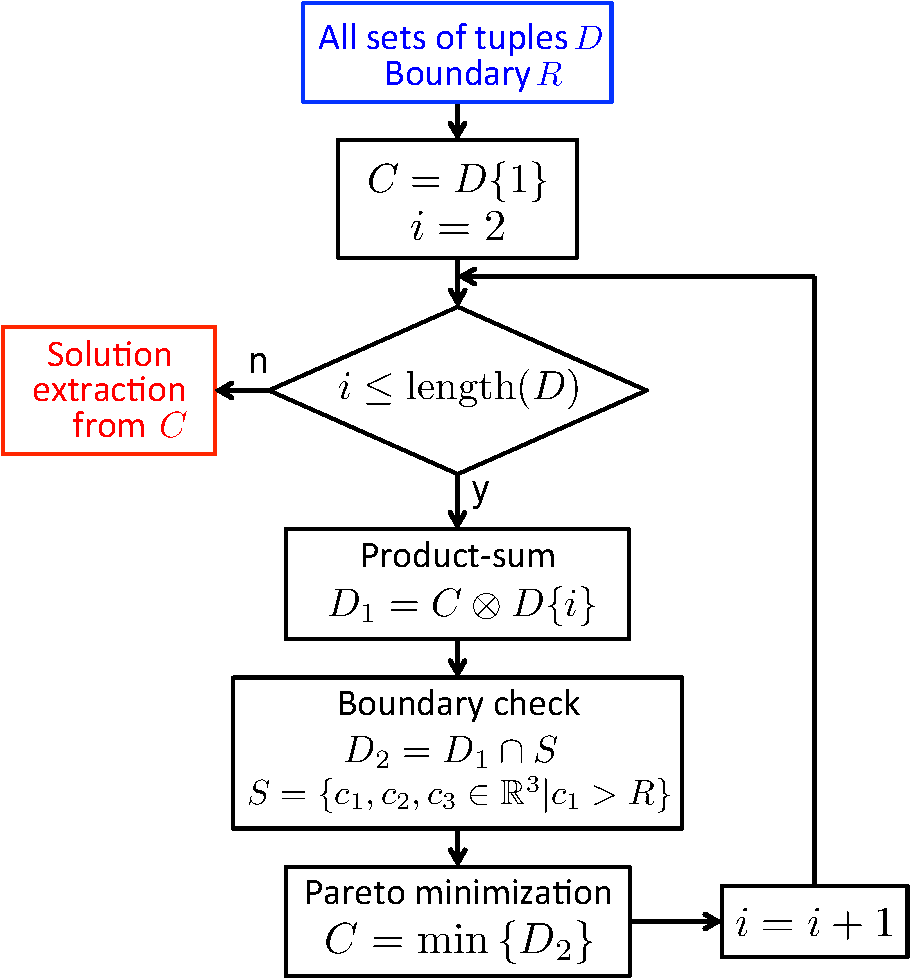
\includegraphics[width=0.55\textwidth]{./chapters/chapter4/images/CPHschema.pdf} 
\caption{CPH algorithm flowchart. All sets of tuples are saved in cell $D$. After the last iteration, the solution is extracted by selecting a tuple in $C$ with the least value of the third dimension.} 
\label{fig:SS2b} 
\end{figure}
In the second step, the sets of tuples are pairwise and iteratively combined by a so-called \textit{product-sum} operation~$\otimes$, which takes all possible combinations from two sets, sums their first and second elements per dimension and then calculates the third element by Eq.~\eqref{eqCPH1}. Some of the partial solutions will be discarded in the third step by two criteria. The first criterion to reject a tuple is that its power demand violates the bound $R$ (rule~1), denoted by the operation $(D_1 \otimes D_2)\cap S$, and the second one is that this tuple is dominated, i.e. it has a greater third value but the same or larger first value than another tuple (rule~2). This process is called \textit{Pareto minimization}~\cite{Shojaei13} and denoted by the operation $C=\min{((D_1 \otimes D_2)\cap S)}$, where $C$ contains the remaining solutions called \textit{Pareto points}. In the final step, after all sets are combined and the Pareto points are found, the point giving the smallest value in the third element is selected as the final solution. 

Figure~\ref{fig:SS2b} resumes the operation of CPH algorithm with
the procedure to combine two sets of tuples presented in Algorithm~\ref{algocph1} and the Pareto minimization illustrated in Algorithm~\ref{algocph2}. The notations $D_1 \preceq D_2$ and $D_1 \prec D_2$ mean that the tuple $D_1$ is dominated and strictly dominated, respectively, by $D_2$.

\begin{algorithm}
\caption{Combine two sets of tuples.} \label{algocph1}
\begin{algorithmic}[1]
\Function{AllComb}{$D_1,D_2,x$}
\State $l1 = \text{length}(D_1)$
\State $l2 = \text{length}(D_2)$
\For {$i=1,\ldots,l1$}
		 \For{$j=1,\ldots,l2$}
		    \State $D\{(i-1)l_1+j\}(1) = D_1\{i\}(1) + D_2\{j\}(1)$
		    \State $D\{(i-1)l_1+j\}(2) = D_1\{i\}(2) + D_2\{j\}(2)$
		    \State $D\{(i-1)l_1+j\}(3) = |D\{(i-1)l_1+j\}(1)-x|+D\{(i-1)l_1+j\}(2)$
		 \EndFor
\EndFor
\State output = $D$
\EndFunction
%\State \textbf{end function}
\end{algorithmic}
\end{algorithm}

\begin{algorithm}
\caption{Pareto minimization.} \label{algocph2}
\begin{algorithmic}[1]
\Function{ParetoMin}{$D,R$}
\State $l = \text{length}(D)$
\State $reject = \text{zeros}(l,1)$
\For {$i=1,\ldots,l$}
    \If {$D\{i\}(1)>R$}
	    \State $reject(i) = 1$
	\EndIf
\EndFor
\State $Ind = \text{find}(reject\neq 1)$
\State $D1 = D\{Ind\}$
\State $l1 = \text{length}(D1)$
\State $reject1 = \text{zeros}(l1,1)$
\For {$i=1,\ldots,l1-1$}
    \For {$j=i+1,\ldots,l1$}
        \If {$reject(j)\neq 1$ and $D1\{i\}\prec D1\{j\}$}
            \State $reject(i)=1$
        \ElsIf {$reject(j)\neq 1$ and $D1\{j\}\preceq D1\{i\}$}
            \State $reject(j)=1$
        \EndIf
    \EndFor
\EndFor
\State $Ind1 = \text{find}(reject1\neq 1)$
\State $D2 = D1\{Ind1\}$
\State output = $D2$
\EndFunction
%\State \textbf{end function}
\end{algorithmic}
\end{algorithm}




\subsubsection{Reed--Solomon codes}\label{DP}
The principle of the DP algorithm to solve the Knapsack problem is that, if the last item is rejected, the best profit will only depend on the remaining items with the full capacity of the knapsack. In contrast, if it is selected, the best profit includes the profit of this item and the best profit obtainable from the remaining items with the remaining capacity of knapsack after subtracting the weight of the last item. 

Therefore, the DP procedure is to construct a profit table with each row corresponding to an item and the number of columns depending on the knapsack capacity with unit step. The profit value of each cell will be calculated based on the current capacity, the corresponding item as well as the recursive relation with the previous cells, which can be explained as follows. At any cell corresponding to an item and a value of capacity, if the item is heavier than the available capacity, it will be rejected and the profit value of the cell is obtained from the previous items. In contrast, it is necessary to compare the profit obtainable with and without that item. The set of the previous items must ensure enough capacity if new item is selected.

\paragraph*{One-state devices}
In the context of one-state devices, each device is considered as an item with its power demand as weight, while the profit is computed from the power demand as well as the operating probability. Although the absolute error between the aggregate power and the total power demand of the identified devices is a criterion to identify the operating devices, it does not satisfy the recursive relation. Concretely,
\begin{eqnarray}
&&\left |\sum_{j=1}^i{w_js_j-x}\right | \neq w_is_i +\left |\sum_{j=1}^{i-1}{w_js_j}-x\right |\\
\mbox{if } &&w_is_i \times \left (\sum_{j=1}^{i-1}{w_js_j}-x\right )<0.\nonumber
\end{eqnarray}

To overcome this restriction, we construct two separated tables, $P^1_e$ and $P^1_l$, for the power and the probability parameters, respectively. Each table is composed of $N$ rows and $R$ columns with $R=\lceil x+\epsilon\rceil$, where $\lceil . \rceil$ is the rounding up operator. The entry of the first table $P^1_e(i,\beta)=\sum_{j=1}^i{w_js_j-x}$ and second table $P^1_l(i,\beta)=\lambda \times \sum_{j=1}^i{L^1(s_j)}$ are calculated by Algorithm~\ref{algo1}. A flag table $F$ is also constructed to mark if a device is running or not.
\begin{algorithm}
\caption{Entry calculation for profit tables in case of one-state devices.}
\label{algo1}
\begin{algorithmic}[1]
\Ensure $P^1_e(i,\beta),P^1_l(i,\beta)$
\State $a^1_1 = P^1_e(i-1,\lfloor \beta-w_i\rfloor)+w_i$
\State $a^1_2 = P^1_l(i-1,\lfloor \beta-w_i\rfloor)+\lambda \times l^1_{i1}$
\State $b^1_1 = P^1_e(i-1,\beta)$
\State $b^1_2 = P^1_l(i-1,\beta)+\lambda \times l^1_{i0}$
\State $A^1 =  \left |a^1_1\right|+a^1_2$
\State $B^1 = \left |b^1_1\right |+b^1_2$
\State $F(i,\beta) = 0$

\If{$w_i \leq \beta$ and $ A^1 \leq B^1$}
  \State $P^1_e(i,\beta) =  a^1_1$
  \State $P^1_l(i,\beta) = a^1_2$
  \State $F(i,\beta) = 1$
\Else
  \State $P^1_e(i,\beta)= b^1_1$
  \State $P^1_l(i,\beta)= b^1_2$
\EndIf
\end{algorithmic}
\end{algorithm}
In Algorithm~\ref{algo1}, because the weight of an item is not an integer number, the notation $\lfloor . \rfloor$ is used to round down the value of $(\beta-w_i)$. The values of $A^1$ and $B^1$ denote the profit obtainable with and without new device in the list of operating ones, respectively. The case that gives better profit is then selected and the respective values are filled in the tables. The initial conditions of each tables are
\begin{eqnarray*}
P^1_e(0,\beta)& =&-x,\beta = 0,\ldots, R\\
P^1_l(0,\beta)& = &0,  \beta = 0,\ldots,R\\
P^1_e(i,0)&=& -x,i=1,\ldots,N\\
P^1_l(i,0) &= &\sum_{j=1}^i{\lambda \times l^1_{j0}},i=1,\ldots,N.
\end{eqnarray*}
After calculating all entries of the profit tables, a backtracking procedure, illustrated in Algorithm~\ref{algo2}, is used to backtrack through the tables from the last cell to obtain the set of running devices with aid of the flag table $F$.

\begin{algorithm}
\caption{Backtracking algorithm in case of one-state devices.}
\label{algo2}
\begin{algorithmic}[1]
\Ensure State indicator vector $\mathbf{s} = \{s_1,\ldots,s_N\}$ 
\State $i = N$
\State $\beta =  R $
\While{$i > 0$ and $\beta>0$}
\If{$P^1_e(i,\beta) \neq P^1_e(i-1,\beta)$ or $F(i,\beta)=1$}
\State $s_i = 1$
\State $\beta = \beta-\lceil w_i \rceil $
\State $i = i-1$
\Else
\State $s_i=0$
\State $i = i-1$
\EndIf
\EndWhile
\end{algorithmic}
\end{algorithm}

Let consider an example for three devices with the respective weight and operating probability: $(w_1,p_1) = (2,0.8)$, $(w_2,p_2) = (5,0.3)$, $(w_3,p_3) = (3.5,0.9)$.
With $P = 10$, $x = 5$, $\epsilon=0.5$, the log-linear form of the operating probability of each device, i.e. $l_{i0} = -\log{(1-p_i)}$ and $l_{i1} = -\log{p_i},i = 1,\ldots,3$, are $(l_{10},l_{11})=(0.7,0.1)$, $(l_{20},l_{21})=(0.15,0.52)$, $(l_{30},l_{31})=(1,0.05)$, respectively, and the boundary of total power $R$ is equal to 6.

The entries of the profit tables are calculated by Algorithm~\ref{algo1} and filled in Table~\ref{table:DP1}. The best profit is obtained at $(i,\beta)=(N,R)$. From this optimal point, the respective combination of running devices can be determined by backtracking through the table by applying Algorithm~\ref{algo2}. As a result, $\mathbf{s} = (1,0,1)$, i.e. the first and third devices are operating while the second one is turned off. Apparently, this combination of devices gives the least absolute error on the power as well as the maximum operating probability.

\begin{table}
\caption{Running example of DP in SmartSense for one-state devices}\label{table:DP1}
\begin{center}
\begin{tabular}{|c|c|c|c|c|c|c|c|}
\hline
\multicolumn{8}{|c|}{$P^1_e(i,\beta)$}\\ \hline 
$(i,\beta)$&0&1&2&3&4&5&6\\ \hline
0&-5&-5&-5&-5&-5&-5&-5 \\ \hline
1&-5&-5&-3&-3&-3&-3&-3 \\ \hline
2&-5&-5&-3&-3&-3&-3&-3 \\ \hline
3&-5&-5&-3&-3&-1.5&-1.5&-0.5 \\ \hline
\multicolumn{8}{|c|}{$P^1_l(i,\beta)$}\\ \hline 
$(i,\beta)$&0&1&2&3&4&5&6\\ \hline
0&0&0&0&0&0&0&0 \\ \hline
1&7&7&1&1&1&1&1\\ \hline
2&8.5&8.5&2.5&2.5&2.5&2.5&2.5\\ \hline
3&18.5&18.5&12.5&12.5&9&9&3\\ \hline
\end{tabular}
\end{center}
\end{table}



\paragraph*{Multi-state devices}

Each multi-state device is considered as a group of items, in which each state is an item with individual weight and profit. Similar to the case of one-state devices, two tables, $P^M_e$ and $P^M_l$, are also constructed to contain the power and probability parameters of the profit. The algorithm to calculate the entries of the first table, $P^M_e(i,\beta)=\sum_{j=1}^i{\sum_{m=1}^{m_i}{(w_{jm}s_{jm}}-x)}$, and the second one, $P^M_l(i,\beta)=P\times \sum_{j=1}^i{L^M(\mathbf{s}_j)},i=1,\ldots,N,\beta=1,\ldots,R$, is detailed in Algorithm~\ref{algo3}. 

\begin{figure}[h]
\centering
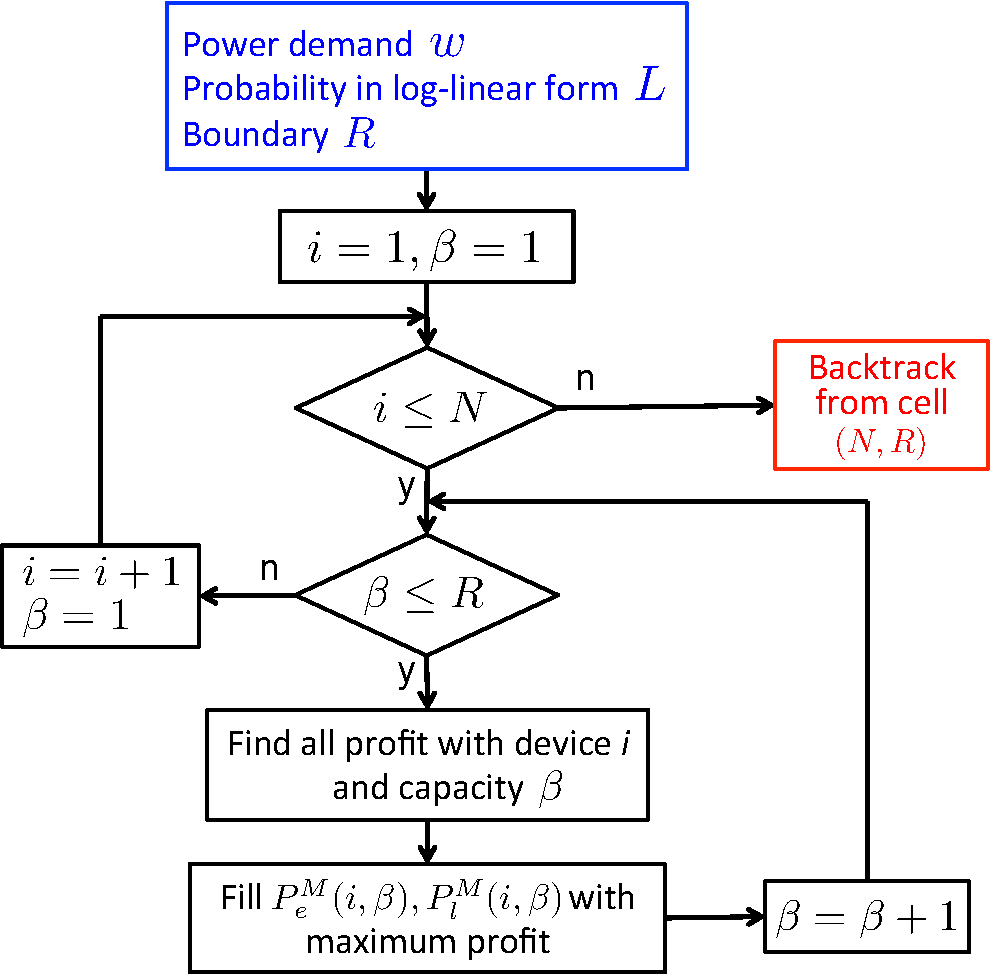
\includegraphics[width=0.6\textwidth]{./chapters/chapter4/images/DPschema.pdf} 
\caption{DP algorithm flowchart. When all entries are filled, the corresponding state vector is obtained by backtracking through the profit tables from the last cell (optimal value).} 
\label{fig:DP1} 
\end{figure}

\begin{algorithm}
\caption{Entry calculation for profit tables in case of multi-state devices.}
\label{algo3}
\begin{algorithmic}[1]
\Ensure $P^M_e(i,\beta),P^M_l(i,\beta)$
\State $Sol(i,\beta) = 0$
\State $a^M_1 = P^M_e(i-1,\beta)$
\State $a^M_2 = P^M_l(i-1,\beta) + \lambda \times l^M_{i0}$
\State $A^M =  \left|a^M_1\right|+a^M_2$
\For{$j=1,\ldots,m_i$}
\If{$w_{ij}\leq \beta$}
\State $b^M_{j1} = P^M_e(i-1,\lfloor \beta-w_{ij}\rfloor)+w_{ij}$
\State $b^M_{j2} = P^M_l(i-1,\lfloor \beta-w_{ij}\rfloor)+\lambda \times l^M_{ij}$
\State $b^M_j = \left|b^M_{j1}\right|+b^M_{j2}$
\Else
\State $b^M_j = +\infty$
\EndIf
\EndFor
\State $k = \min_j{\{b^M_j\}}$; $B^M = b^M_k$
\If{$\min_j{\{w_{ij}\}}\leq \beta$ and $A^M \leq B^M$}
  \State $P^M_e(i,\beta) = a^M_1$
  \State $P^M_l(i,\beta) = a^M_2 $
  \Else
  \State $P^M_e(i,\beta) = b^M_{k1}$
  \State $P^M_l(i,\beta) = b^M_{k2}$
  \State $Sol(i,\beta) = k$
\EndIf
\end{algorithmic}
\end{algorithm}
In other words, the value of each entry when considering a new device is determined by comparing the obtainable profit in two cases: the device is turned off, with profit $A^M$ and the device is operating at a state satisfying the capacity $\beta$, with profit $B^M$.
The initial conditions of the profit tables are
\begin{eqnarray*}
P^M_e(0,\beta) &=& -x,\beta=0,\ldots,R \\
P^M_l(0,\beta)&=&0,\beta = 0,\ldots,R\\
P^M_e(i,0) &=& -x,i=1,\ldots,N\\
P^M_l(i,0)&=&\sum_{j=1}^i{l^M_{j0}},i=1,\ldots,N.
\end{eqnarray*}

To get the state of each device, a backtracking procedure is also constructed as illustrated in Algorithm~\ref{algo4}, in which an additional table $Sol$ with the same size as the profit tables is used to mark the state of devices corresponding to each cell of profit tables.

\begin{algorithm}
\caption{Backtracking algorithm in case of multi-state devices.}
\label{algo4}
\begin{algorithmic}[1]
\Ensure State indicator vector $\mathbf{s} = \{s_1,\ldots,s_N\}$
\State $i = N$ 
\State $\beta =  R$
\While{$i > 0$ and $\beta>0$}
\If{$Sol(i,\beta)>0$}
\State $k = Sol(i,\beta)$
\State $s_i = k$
\State $\beta = \beta-\lceil w_{ik} \rceil $
\State $i = i-1$
\Else
\State $s_i=0$\; $i = i-1$
\EndIf
\EndWhile
\end{algorithmic}
\end{algorithm}

Figure~\ref{fig:DP1} illustrates the flowchart of the proposed DP algorithm in the general case with multi-state devices. Meanwhile, Table~\ref{table:DP2} shows the profit tables relating to the DP algorithm for three multi-state devices with the individual power demand $w_{11}=2$, $(w_{21},w_{22})=(1,4)$, $(w_{31},w_{32}) = (3,5)$ and the respective operating probability $p_{11} = 0.8$, $(p_{21},p_{22}) = (0.7,0.2)$, $(p_{31},p_{32}) = (0.6,0.2)$. The aggregate power consumption $x$ in this example is equal to 6 with standard deviation $\epsilon=0$ and the respective total power boundary $R = \lceil x+\epsilon \rceil = 6$. The regularization parameter $P$ is set to be of $10$. Applying the log-linear form to the operating probability, i.e. $l_{ij} = -\log{p_{ij}},i=1,\ldots,3,j=0,\ldots,m_i$, the corresponding results are $(l_{10},l_{11}) = (0.7,0.1)$, $(l_{20},l_{21},l_{22}) = (1, 0.15, 0.7)$, $(l_{30},l_{31},l_{32}) = (0.7,0.22,0.7)$. Each entry of these tables is calculated by Algorithm~\ref{algo3} and the set of operating state of each device is backtracked through the tables from the optimal point, i.e. $(i,\beta) = (N,R)$, by applying Algorithm~\ref{algo4} is then $\mathbf{s} = (1,1,1)$. This result means that all three devices are operating at the first power state. This determination also satisfies the requirement on the least absolute error on the power consumption and the maximum coincidence operating probability. Presenting vector $\mathbf{s}$ as in Eq.~\ref{eqSS12}, we have $\mathbf{s} = \{1,1,0,1,0\}$.
\begin{table}
\caption{Running example of DP in SmartSense for multi-state devices}\label{table:DP2}
\begin{center}
\begin{tabular}{|c|c|c|c|c|c|c|c|}
\hline
\multicolumn{8}{|c|}{$P^M_e(i,\beta)$}\\ \hline 
$(i,\beta)$&0&1&2&3&4&5&6\\ \hline
0&-6&-6&-6&-6&-6&-6&-6 \\ \hline
1&-6&-6&-4&-4&-4&-4&-4 \\ \hline
2&-6&-5&-5&-3&-3&-3&-3 \\ \hline
3&-6&-5&-5&-3&-3&-3&0 \\ \hline
\multicolumn{8}{|c|}{$P^M_l(i,\beta)$}\\ \hline 
$(i,\beta)$&0&1&2&3&4&5&6\\ \hline
0&0&0&0&0&0&0&0 \\ \hline
1&7&7&1&1&1&1&1\\ \hline
2&17&8.5&8.5&2.5&2.5&2.5&2.5\\ \hline
3&24&15.5&15.5&9.5&9.5&9.5&4.7\\ \hline
\end{tabular}
\end{center}
\end{table}







\section{Energy and power savings from ECC}
The edge detector was firstly proposed in \cite{Hart92} to detect the step-changes on the power signal. Both ED and DTW algorithms at first try to detect the rising edge and falling edge of a device activation and pair them together. Denote $\Delta x(t) = x(t) - x(t-1)$, a rising edge is detected at time $t$ if
$\Delta x(t)\geq \gamma$,
where $\gamma$ is empirically chosen so that it is small enough not to miss the edges, but large enough to ignore the variations in a stable period. In contrast, a falling edge is detected at time $(t-1)$ if $\Delta x(t)\leq -\gamma$. A rising edge and a falling edge are paired together if the difference between their height is lower than a threshold $\alpha$, i.e.,
\begin{equation}
|\Delta x(t_s) - |\Delta x(t_e)||\leq \alpha.
\end{equation}
In the case of multi-state devices, it appears more than one consecutive rising edges or falling edges in an activation. These edges will be grouped together if
\begin{eqnarray}
\left|\sum_{i=1}^{n_s}{\Delta x(t_s^i)}-\left |\sum_{i=1}^{n_e}{\Delta x(t_e^i)}\right| \right|\leq \alpha,
\end{eqnarray}
where $n_s$, $n_e$ are the number of consecutive rising edges and falling edges, respectively.

In the ED algorithm, a feature is composed of the first rising edge and the last falling edge, while all active power values between them are used in DTW feature. To improve the performance of the edge detector, a median filter can also be applied to remove the peaks~\cite{Norford96,Marceau2000ECM}.

\subsection{Results}
In training period, all possible patterns of each device are extracted and saved in the library $\mathbf{EDlib}$, in which pattern $j$ of device $i$ is denoted as 
\begin{equation}
f_{ij}^{ed} = \{\Delta x_{ij}^R,\Delta x_{ij}^F\},
\end{equation}
with notation $R$ for rising edge and $F$ for falling edge.
If the edge detector detects an event switched on at time $t_s$ and switched off at time $t_e$, the corresponding feature is
\begin{equation}
f^{ed} = \{\Delta x(t_s^1),\Delta x(t_e^{n_e})\}.
\end{equation}
The distance between two patterns $f_{ij}^{ed}$ and $f^{ed}$ can be calculated as
\begin{eqnarray}\label{eqED1}
\delta_{ij}^{ed} &=& d(f^{ed},f_{ij}^{ed})\nonumber \\
&=&|\Delta x(t_s^1)-\Delta x_{ij}^R|+|\Delta x(t_e^{n_e})-\Delta x_{ij}^F|.
\end{eqnarray}
In the ED algorithm, the detected event will be matched with the device having a pattern with the minimum distance. Nevertheless, in homes and buildings, there are several devices with the same edge height, which decreases the load disaggregation performance. To overcome this challenge, in SmartSense, the probability that each device $i, i=1,\ldots,N$, is turned on and off at the same time as the detected event, denoted as $p_i^R(t_s^1)$ and $p_i^F(t_e^{n_e})$, respectively, is estimated as in Section~\ref{model}. This means, $p_i^R(t_s^1)=(1-npv)$ if a rising edge of device $i$ is detected at time $t_s^1$ and $p_i^R(t_s^1)=(1-npv)$ on the contrary. Similarly, $p_i^F(t_e^{n_e})=pr$ if device $i$ has a falling edge at time $t_e^{n_e}$ and $p_i^F(t_e^{n_e})=(1-npv)$ on the contrary. In the case of unsupervised devices, $p_i^R(t_s^1) = p_i^F(t_e^{n_e}) = 0.5$. The coincidence probability that both edges appear is then
\begin{equation}\label{eqED2}
Pr_i^{ed} = p_i^R(t_s^1)\times p_i^F(t_e^{n_e}).
\end{equation}

To reduce the computational complexity, the multiplication in Eq.~\eqref{eqED2} can be transformed to an addition by applying the log-linear form, which gives
\begin{eqnarray}\label{eqED3}
\phi_i^{ed} &=& -\log{Pr_i^{ed}}\nonumber \\
&=& -\log{p_i^R(t_s^1)}-\log{p_i^F(t_e^{n_e})}.
\end{eqnarray}
The identified device does not only have a pattern with the minimum distance $\delta_{ij}^{ed}$, but also has the maximum probability $Pr_i^{ed}$, i.e. the minimum log-linear form $\phi_i^{ed}$. In other words, the ED algorithm will try to find the pattern giving the minimum modified distance, calculated as
\begin{eqnarray}
d_{ij}^{ed} = \delta_{ij}^{ed}+\lambda_1\times \phi_i^{ed},
\end{eqnarray}
where $\lambda_1$ is a regularization parameter. The load identification procedure for each detected pattern is presented in Algorithm~\ref{algo:ED1}, where $\Phi^{ed}$ contains the probability in log-linear form of all devices and $m_i$ denotes the number of patterns of device $i$ in $\mathbf{EDlib}$. The procedure is illustrated by a flowchart in Figure~\ref{fig:ed1}.
\begin{figure}[!h]
\centering
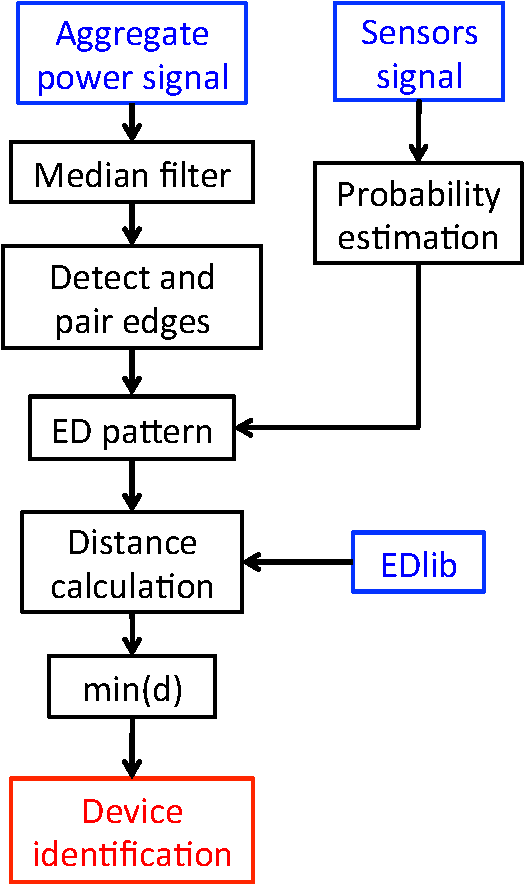
\includegraphics[width=0.45\textwidth]{./chapters/chapter4/images/EDschema.pdf} 
\caption{Load disaggregation based on the ED algorithm.} 
\label{fig:ed1} 
\end{figure}

\begin{algorithm}
\caption{Matching detected event in ED.}\label{algo:ED1}
\begin{algorithmic}[1]
\Function{EDiden}{$f^{ed},\Phi^{ed},\mathbf{EDlib}$}
\State $MIN = +\infty$
\State $k = 0$
	\For {$i=1,\ldots,N$}
	    \State{$\phi^{ed}_i=\Phi^{ed}(i)$}
		 \For{$j=1,\ldots,m_i$}
		    \State $f_{ij}^{ed} = \mathbf{EDlib}\{i,j\}$
		    \State $\delta_{ij}^{ed} = |\Delta x(t_s^1)-\Delta x_{ij}^R|+|\Delta x(t_e^{n_e})-\Delta x_{ij}^F|$
		    \State $d_{ij}^{ed} = \delta_{ij}^{ed}+\lambda_1\times \phi_i^{ed}$
		    \If{$d_{ij}^{ed}\leq MIN$}
		        \State $MIN = d_{ij}^{ed}$
		        \State $k = i$
		    \EndIf
		 \EndFor
	\EndFor
	%\State \textbf{end for}
\State output = $k$
\EndFunction
%\State \textbf{end function}
\end{algorithmic}
\end{algorithm}



\subsection{Analyzing}
Different from the ED algorithm, in DTW, all active power values between the first rising edge and the last falling edge are extracted to comprise a pattern, i.e. $f^{dtw}=\{f^{dtw}(k)|k=1,\dots,t_e^{n_e}-t_s^1+1\}$, which
\begin{eqnarray}
f^{dtw}(k)=\begin{cases}
h_s^i, & z_s^i\leq k <z_s^{i+1},1\leq i \leq n_s-1\\
h_s^{n_s}+\frac{h_e^1-h_s^{n_s}}{z_e^1-z_s^{n_s}}\left(k-z_s^{n_s} \right), & z_s^{n_s}\leq k \leq z_e^1\\
h_s^{i+1}, & z_e^i < k \leq z_e^{i+1},1< i\leq n_e-1
\end{cases}
\end{eqnarray}
where $h_s^i = \sum_{j=1}^i{\Delta x(t_s^j)}$, $h_e^i=\left|\sum_{j=i}^{n_e}{\Delta x(t_e^j)}\right|$, $z_s^i=t_s^i-t_s^1+1$, and $z_e^i=t_e^i-t_s^1+1$.
Figure~\ref{fig:dtw2} illustrates a DTW pattern with two rising edges and two falling edges.
\begin{figure}[!h]
\centering
\centerline{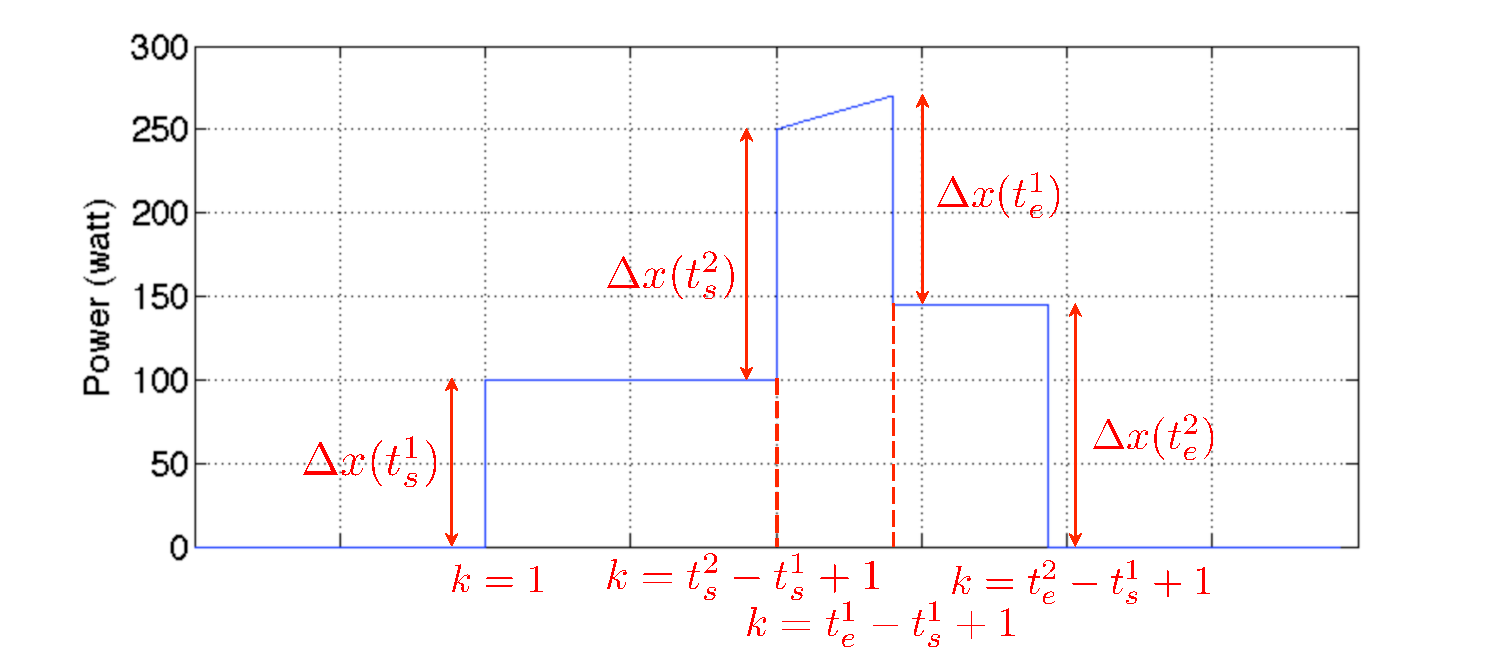
\includegraphics[width=0.8\textwidth]{./chapters/chapter4/images/dtwpattern.pdf}}
\caption{DTW pattern.}
\label{fig:dtw2}
%
\end{figure}
All possible patterns of each device are extracted and saved in library $\mathbf{DTWlib}$ from the training period. Because the length of patterns is different, the accumulated distance between the detected pattern $f^{dtw}$ and a pattern $j$ of device $i$ in the library is calculated by Algorithm~\ref{algo:DTW1}. Concretely,
\begin{equation}\label{eqDTW1}
\delta_{ij}^{dtw} = AccDistance(f^{dtw},f_{ij}^{dtw}).
\end{equation}
\begin{algorithm}
\caption{Accumulated distance between two different length vectors~\cite{Liao14}.} \label{algo:DTW1}
\begin{algorithmic}[1]
\Function{AccDistance}{$f1,f2$}
\State $l1 = \text{length}(f1)$
\State $l2 = \text{length}(f2)$
\State $\delta(0,0) = 0;\delta(i,0) = \delta(0,i) = +\infty$
	\For {$i=1,\ldots,l1$}
		 \For{$j=1,\ldots,l2$}
		    \State $d(i,j) = |f1(i)-f2(j)|$
		    \State $\delta(i,j) = d(i,j)+\min{\{\delta(i-1,j),\delta(i-1,j-1),\delta(i,j-1)\}}$
		 \EndFor
	\EndFor
	%\State \textbf{end for}
\State output = $\delta(l1,l2)$
\EndFunction
%\State \textbf{end function}
\end{algorithmic}
\end{algorithm}

In~\cite{Liao14}, the detected pattern will be matched to the device having a pattern with minimum accumulated distance calculated by Eq.~\eqref{eqDTW1}. 
However, in SmartSense, in order to improve the performance, the operating probability of each device during the same period as the detected event will also be used in log-linear form, and is defined as
\begin{eqnarray}
Pr_i^{dtw} &=& \prod_{t=t_s^1}^{t_e^{n_e}}{p_i(t)}\\
\phi_i^{dtw} &=& -\log{Pr_i^{dtw}}\nonumber \\
&=& -\sum_{t=t_s^1}^{t_e^{n_e}}{\log{p_i(t)}},\label{eqDTW2}
\end{eqnarray}
where $p_i(t)$ is the on-state probability of device $i$ at time instant $t$, estimated as in Section~\ref{model}, i.e. $p_i(t) =pr$ if device $i$ is detected as on and $p_i(t) = (1-npv)$ if detected as off. In the case of unsupervised devices, $p_i(t) = 0.5$. The load identification, as presented in Algorithm~\ref{algo:DTW2}, is not only based on the accumulated distance as in Eq.~\eqref{eqDTW1}, but also considers the operating probability of each device in Eq.~\eqref{eqDTW2}. The probability in log-linear form of all devices is contained in vector $\Phi^{dtw}$. A modified distance then combines these two parameters with a regularization parameter $\lambda_2$, which gives
\begin{equation}
d_{ij}^{dtw} = \delta_{ij}^{dtw} + \lambda_s\times \phi_i^{dtw}.
\end{equation}
The pattern giving the minimum distance will be selected to identify the corresponding device. Because the length of patterns strongly affects the accumulated distance, the DTW algorithm is only suitable for devices with fixed on-duration, such as fridge, washing machine, dish washer. Other devices controlled by the human intervention, e.g. lamp, computer, etc., cannot be exactly identified. Therefore, we propose to combine DTW with ED, in which $\mathbf{DTWlib}$ only contains the patterns of fixed on-duration devices and $\mathbf{EDlib}$ saves the edge patterns of the others. The flowchart of the proposed DTW algorithm is shown in Figure~\ref{fig:dtw1}. A threshold $\beta$ is used to reject a DTW pattern if it does not match with any one in $\mathbf{DTWlib}$. The detected pattern will be then extracted based only on the first rising edge and the last falling edge, by applying the ED procedure.
\begin{algorithm}
\caption{Matching detected event in DTW.}\label{algo:DTW2}
\begin{algorithmic}[1]
\Function{DTWiden}{$f^{dtw},\Phi^{dtw},\mathbf{DTWlib}$}
\State $MIN = +\infty$
\State $k = 0$
	\For {$i=1,\ldots,N$}
	    \State{$\phi_i^{dtw}=\Phi^{dtw}(i)$}
		 \For{$j=1,\ldots,m_i$}
		    \State $f_{ij}^{dtw} = \mathbf{DTWlib}\{i,j\}$
		    \State $\delta_{ij}^{dtw} = AccDistance(f^{dtw},f_{ij}^{dtw})$
		    \State $d_{ij}^{dtw} = \delta_{ij}^{dtw} + \lambda_2\times \phi_i^{dtw}$
		    \If{$d_{ij}^{dtw}\leq \beta$ and $d_{ij}^{dtw}\leq MIN$}
		        \State $MIN = d_{ij}^{dtw}$
		        \State $k = i$
		    \EndIf
		 \EndFor
	\EndFor
	%\State \textbf{end for}
\State output = $k$
\EndFunction
%\State \textbf{end function}
\end{algorithmic}
\end{algorithm}

\begin{figure}[!ht]
\centering
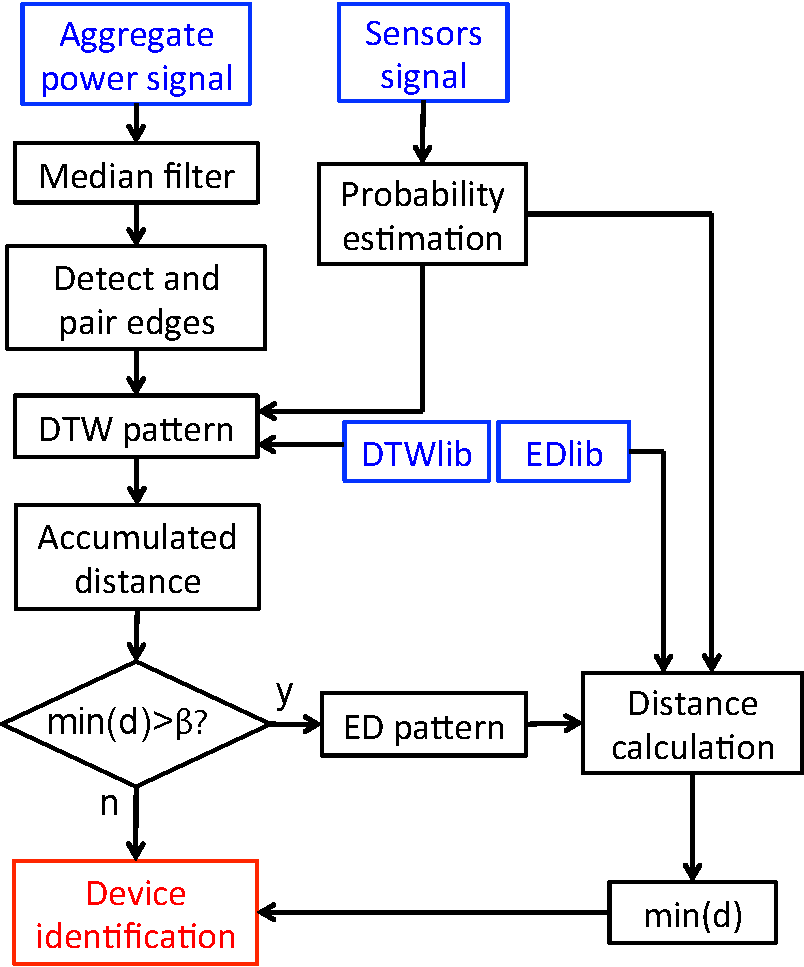
\includegraphics[width=0.65\textwidth]{./chapters/chapter4/images/DTWschema.pdf} 
\caption{Combination of DTW and ED algorithms. A threshold $\beta$ is used to reject a pattern if it does not match with any one in $\mathbf{DTWlib}$} 
\label{fig:dtw1} 
\end{figure}


\section{Conclusion}


\chapter{Optical Network Interface Design} % Write in your own chapter title
\label{ResultsSS}
%\addtotoc{State of the Arts}
\lhead{\emph{Experimental Results on SmartSense}} % Write in your own chapter title to set the page header
%\section{Experimental Results}
\section{Introduction}
In the context of this thesis, the sensor signal processing to extract the state of devices is not studied nor implemented. We just focus on how to transform this information to probability feature to help the existing NILM algorithms to improve their performance. Therefore, with each dataset applied to the simulation in Matlab, we assume a WSN monitoring some specific devices. The operation of these devices can be detected with a certain accuracy.
To evaluate the WSN performance, besides the precision, recall, F-measure introduced in Chapter~\ref{l1norm} and negative predictive value as in Section~\ref{model}, another metric called \textit{true negative rate} ($tnr$) is also used and calculated as follows:
\begin{eqnarray}
tnr &= &\frac{TN}{TN+FP}.
\end{eqnarray}
Denote $r$ as the ratio between the total events and total non-events of the data, the true negative rate and negative predictive value are calculated as functions of precision and recall, such as:
\begin{eqnarray}
tnr &=& 1-\frac{rc\times r\times (1-pr)}{pr} \\
npv &=& 1-\frac{pr\times r\times (1-rc)}{pr \times (1+r)-rc\times r}.
\end{eqnarray}
Knowing the characteristics of the sensor network, the data of individual circuits can be modified to apply in SmartSense. Whereby, $(1-rc)$ of events are randomly selected and changed to non-events, and in contrast, $(1-tnr)$ of non-events are randomly selected and changed to events. At these instants, the corresponding devices are assumed to be incorrectly detected.
As a consequence, the operating probability of each device will be determined from the modified data based on the precision and negative predictive value as presented in Section~\ref{model}.
\section{Target Architecture and Principle}
In the simulation, the proposed algorithms are applied to four datasets: UK-DALE House~5 (UK-DALE~5)~\cite{UK-DALE}, REDD House 1 (REDD~1) and House 2 (REDD~2)~\cite{Kolter11redd}, and our Athemium dataset retrieved from the coffee room as introduced in Chapter~\ref{l1norm}. The devices as well as their characteristics in each dataset are detailed in Tables \ref{table:SR1}, \ref{table:SR2}, \ref{table:SR3} and \ref{table:SR4}, respectively. Both UK-DALE and REDD public datasets are retrieved by measuring the power consumption at the main power line and of several typical devices in home sampled every 3-4 seconds.
Although there are over 20 channels in each dataset, we use only a part of them because the others have no activation and the variable loads are ignored. In addition, the data from two main phases in REDD dataset are also combined to have a unique main power signal. The data in each dataset are divided into two parts: the first one (30$\%$) to train the power characteristics of each device and the second one (70$\%$) to test the algorithms. During the training period, the \textit{ghost power}, coming from the unsupervised devices, is assumed to be consumed by a virtual device. 


\begin{table}
\caption{List of devices in REDD~1 and their characteristics.}\label{table:SR1}
\begin{center}
\begin{tabular}{|c|c|c|c|c|c|c|c|}

\hline
 Label & Device& \shortstack{Number of uses} &\shortstack{Using rate (\%)}&Power (watts)\\
 \hline 
 1 & Oven & 153 &0.24& $\{4140, 4075,3377\}$\\
 \hline
 2 & Fridge  & 1695 &24.94& $\{193,423\}$\\
 \hline
 3&Dish washer & 383&3.80& $\{214,1107\}$ \\
 \hline
 4& Lighting &67&48.99&$\{169,275,345\}$\\
 \hline
 5& Microwave   &522&1.94& $\{1531,1571,1396\}$\\
 \hline
 6& Outlet bathroom  & 226&0.39& 1595\\
 \hline
 7& Outlet  & 189&0.38&1056\\
 \hline
 8&Outlet&90&0.2&1521\\
 \hline
 9&Washer dryer&234&0.76&$\{5097,5250,5008\}$\\
 \hline
\end{tabular}
\end{center}
\end{table}

\begin{table}
\caption{List of devices in REDD~2 and their characteristics.}\label{table:SR2}
\begin{center}
\begin{tabular}{|c|c|c|c|c|c|c|c|}

\hline
  Label & Device  & \shortstack{Number of uses} &\shortstack{Using rate (\%)}&Power (watts)\\
 \hline 
 1 & Outlet   & 180 &0.25& 779 \\
 \hline
 2 & Lighting   & 275 &12.67& $\{153,71\}$ \\
 \hline
 3&Stove & 63 &0.22& 406 \\
 \hline
 4& Microwave  & 120 &0.69& $\{1887,1778\}$\\
 \hline
 5&Outlet&126 &0.86&$1058$\\
 \hline
 6& Fridge  & 2715 &44.40&$\{163,426\}$\\
 \hline
 7&Dish washer&207 &1.19&$\{244,1214\}$\\
 \hline
\end{tabular}
\end{center}
\end{table}
\subsection{Electrical -- Optical Interface}
\begin{table}
\caption{List of devices in UK-DALE~5 and their characteristics.}\label{table:SR3}
\begin{center}
\begin{tabular}{|c|c|c|c|c|c|c|c|}

\hline
 Label & Device  & \shortstack{Number of uses} &\shortstack{Using rate (\%)}&Power (watts)\\
\hline 
1 & Toaster & 162 &0.06 &  1088\\
\hline
2& Kettle &  1013 &0.37 &$\{2826,2960\}$\\
\hline
3& Fridge & 8312 & 36.48 & 109.5\\
\hline
4 & Oven & 4268 & 22.56 &  $\{110.6, 2119,2933\}$\\
\hline
5 & Electric hob & 2260 & 0.52 & $\{961,1878,1611\}$\\
\hline
6 & Dish washer & 365 & 2.38 & $\{1660,96.3,57.4\}$\\
\hline
7& Microwave & 186 & 68.40&$\{1496,1258,49.8\}$\\
\hline
8 & Washer dryer & 5942 & 2.89 & $\{61.7,1492,290.6\}$\\
\hline
\end{tabular}
\end{center}
\end{table}
\subsection{Optical -- Electrical Interface}
\begin{table}
\caption{List of devices in Athemium dataset and their characteristics.}\label{table:SR4}
\begin{center}
\begin{tabular}{|c|c|c|c|c|c|c|c|}

\hline
  Label & Device  & \shortstack{Number of uses} &\shortstack{Using rate (\%)}&Power (watts)\\
 \hline 
1&Fridge & 3040 & 17.79 & 75\\
\hline
2& Coffee machine & 1345 & 1.57 & $\{823,798,234\}$ \\
\hline
3& Teapot & 640 & 0.94 & $\{1635,1692\}$\\
\hline 
4& Microwave & 250 & 0.24 & $\{1290,1349\}$\\
\hline
5& Television & 70 & 35.76 & $\{203,29\}$\\
\hline
6& Monitor & 110 & 27.35 & 73\\
\hline
\end{tabular}
\end{center}
\end{table}

The simulation with the training data also allows to empirically choose the value of the regularization parameters, as shown in Table~\ref{table:SR5}.

\begin{table}
\caption{Regularization parameters.}\label{table:SR5}
\begin{center}
\begin{tabular}{|c|c|c|c|c|c|c|c|}

\hline
 & $\alpha$  & $\beta$ & $\gamma$ & $\delta$ & $\lambda$ & $\epsilon$ &$L$\\
\hline 
CPH & & & & & 60 & 20 &128\\
\hline
DP & & & &10 & 60 & 20& \\
\hline
DTW & & 500 & 60 & & 2 & & \\
\hline
ED & 30 & & 60 & & 10 & & \\
\hline
\end{tabular}
\end{center}
\end{table}








\section{Results and Evaluation of Optical Network Interface}

\subsection{Methodology}

To evaluate the effect of the probability information on the performance improvement of NILM algorithms, we consider the gain obtained by comparing the overall performance of each algorithm without monitored device. The performance of the algorithms without probability information are provided in Table~\ref{table:SR6}. In an original NILM system, both DTW and ED algorithms show a better performance than the CPH and DP ones. Not only that, in \cite{Liao14}, DTW is proved to outperform other state-of-the-art approaches when applied to REDD dataset. 
\begin{table}
\caption{Performance of the algorithms without monitored device~($\%$).}\label{table:SR6}
\begin{center}
\begin{tabular}{|c|c|c|c|c|c|c|}
\hline
 & \multicolumn{3}{c|}{REDD~1}&\multicolumn{3}{c|}{REDD~2}\\
 \hline
 & \shortstack{$pr_0$} &\shortstack{$rc_0$} &\shortstack{$Fm_0$} & \shortstack{$pr_0$} & \shortstack{$rc_0$} & \shortstack{$Fm_0$} \\
 \hline
 CPH & 61.09& 65.12 & 63.04 &66.64 & 74.21 & 70.22\\
 \hline
 DP & 61.34& 65.11 & 63.17 & 67.18 & 73.49 & 70.19  \\
 \hline
 DTW & 83.53 & 76.48  & 79.85  & 83.77  & 76.50 & 79.97 \\
 \hline
 ED & 80.95 & 70.58 & 75.41 &83.71 & 68.32 & 75.24\\
 \hline
 \multicolumn{7}{c}{}\\
\hline
 & \multicolumn{3}{c|}{UK-DALE~5}&\multicolumn{3}{c|}{Athemium}\\
  \hline
 & \shortstack{$pr_0$} &\shortstack{$rc_0$} &\shortstack{$Fm_0$} & \shortstack{$pr_0$} & \shortstack{$rc_0$} & \shortstack{$Fm_0$} \\
 \hline
 CPH & 66.88 & 59.19 & 62.80 & 65.51 & 71.25  & 68.26 \\
 \hline
 DP &68.67 & 59.48 & 63.74 & 65.92 & 71.10 & 68.41   \\
 \hline
\end{tabular}
\end{center}
\end{table}

%==================
\begin{table}
\caption{Performance per device in REDD~1 without monitored device~($\%$).}\label{table:SR6a}
\begin{center}
\begin{tabular}{|c|c|c|c|c|c|c|c|c|c|c|}
\hline
\multicolumn{2}{|c|}{Device}& 1&2&3&4&5&6&7&8&9\\
\hline
\multirow{3}{*}{CPH} & $pr_0$ &26.49&62.13&23.83&77.02&26.01&19.16&13.14&24.46&80.25 \\
& $rc_0$ &49.71&57.78&69.28&71.86&16.07&20.52&21.57&18.14&70.67 \\
& $Fm_0$ & 34.57&59.88&35.48&74.35&19.86&19.82&16.33&20.83&75.16\\
\hline
\multirow{3}{*}{DP} & $pr_0$ & 48.27&58.62&24.09&73.49&25.87&15.84&18.22&13.82&90.31 \\
& $rc_0$ & 35.61&34.80&70.23&71.85&40.51&24.19&23.17&35.71&71.17 \\
& $Fm_0$ &40.99&43.67&35.87&72.66&31.58&19.14&20.40&19.92&79.61 \\
\hline
\multirow{3}{*}{ED} & $pr_0$ & 42.88&89.70&79.47&34.85&28.85&40.52&49.27&19.16&90.75\\
& $rc_0$ &59.66&78.32&51.48&25.05&58.01&61.90&43.21&17.45&54.18  \\
& $Fm_0$ &49.89&83.62&62.48&29.15&38.53&48.98&46.04&18.26&67.85 \\
\hline
\multirow{3}{*}{DTW} & $pr_0$ &47.54 &85.39 &78.85 &68.81 &34.17 &39.74 &49.27 &21.46 &99.36 \\
& $rc_0$ &74.95 &83.49 &56.19 &25.05 &68.01 &61.90 &43.21 &20.45 &67.61  \\
& $Fm_0$ &58.18 &84.43 &65.62 &36.73 &45.48 &48.40 &46.04 &20.94 &80.47 \\
\hline
\end{tabular}
\end{center}
\end{table}

\begin{table}
\caption{Performance per device in REDD~2 without monitored devices~($\%$).}\label{table:SR6b}
\begin{center}
\begin{tabular}{|c|c|c|c|c|c|c|c|c|}
\hline
\multicolumn{2}{|c|}{Device}& 1&2&3&4&5&6&7\\
\hline
\multirow{3}{*}{CPH} & $pr_0$ & 19.72&26.07&26.17&90.98&29.05&82.40&25.64\\
& $rc_0$ & 22.63&37.09&50.87&16.13&25.62&90.46&51.05  \\
& $Fm_0$ & 21.08&30.62&34.56&27.40&27.23&86.24&34.14 \\
\hline
\multirow{3}{*}{DP} & $pr_0$ & 17.86&26.94&23.93&90.52&24.86&89.06&24.43 \\
& $rc_0$ & 18.37 & 25.06&57.10&11.46 &23.08 & 80.64&48.07  \\
& $Fm_0$ & 18.11&25.97& 33.73&20.34&23.94&84.64&32.40 \\
\hline
\multirow{3}{*}{ED} & $pr_0$ &80.65&93.81&21.55&98.65&60.09&67.60&21.08 \\
& $rc_0$ & 19.65&40.04&95.13&17.62&75.12&83.96&45.66 \\
& $Fm_0$ & 31.60&56.12&35.15&29.90&68.67&71.54&28.83 \\
\hline
\multirow{3}{*}{DTW} & $pr_0$ & 80.65&94.17 &21.55 &52.80 &63.09 &80.57 &27.82 \\
& $rc_0$ &19.65 &39.01 &93.13 &39.04 &85.12 &84.11 &55.15  \\
& $Fm_0$ &31.60 &55.17 &35.01 &44.89 &72.47 &82.30 &36.98  \\
\hline
\end{tabular}
\end{center}
\end{table}


\begin{table}
\caption{Performance per device in UK-DALE~5 without monitored device~($\%$).}\label{table:SR6c}
\begin{center}
\begin{tabular}{|c|c|c|c|c|c|c|c|c|c|}
\hline
\multicolumn{2}{|c|}{Device}& 1&2&3&4&5&6&7&8\\
\hline
\multirow{3}{*}{CPH} & $pr_0$ &11.76&32.82&73.26&26.39&14.67&6.10&86.61&75.25 \\
& $rc_0$ &51.02&38.87&27.04&21.04&44.28&54.05&65.34&62.82  \\
& $Fm_0$ &19.11&35.59&39.50&23.41&22.04&10.97&74.49&68.48 \\
\hline
\multirow{3}{*}{DP} & $pr_0$ &6.23 &39.96 &82.27 &24.17 &14.91 &3.85 &83.76 &88.50 \\
& $rc_0$ &23.62 &53.23 &82.42 &7.30 &52.20 &50.40 &53.90 &65.02  \\
& $Fm_0$ &9.86 &45.65 &82.34 &11.22 &23.20 &7.16 &65.59 &74.97 \\
\hline
\end{tabular}
\end{center}
\end{table}

\begin{table}
\caption{Performance per device in Athemium without monitored device~($\%$).}\label{table:SR6d}
\begin{center}
\begin{tabular}{|c|c|c|c|c|c|c|c|c|c|}
\hline
\multicolumn{2}{|c|}{Device}& 1&2&3&4&5&6\\
\hline
\multirow{3}{*}{CPH} & $pr_0$&48.30&79.78&96.95&54.51&83.84&72.32  \\
& $rc_0$&94.09&99.05&44.92&76.22&97.24&52.47   \\
& $Fm_0$ &63.83&88.38&61.39&63.56&90.04&60.82\\
\hline
\multirow{3}{*}{DP} & $pr_0$ &47.75 &89.34 &99.44 &47.02 &82.29 &85.40  \\
& $rc_0$ &97.11 &98.98 &62.22 &83.99 &97.26 &57.78   \\
& $Fm_0$ &64.02 &93.91 &76.55 &60.29 &89.15 &68.93  \\
\hline
\end{tabular}
\end{center}
\end{table}
%=======================

Additionally, the performance per device is also considered and compared with the traditional NILM system given in Tables~\ref{table:SR6a}, \ref{table:SR6b}, \ref{table:SR6c} and \ref{table:SR6d}. 
Apparently, the performance of the DTW algorithm in terms of F-measure related to the devices with fixed on-duration is improved compared with the ED one. For example in REDD~1, the fridge (device 2) is detected with a precision of 89.7$\%$ and recall of 78.32$\%$ by the ED algorithm. Although the DTW method can only identify it with a lower reliability (85.39$\%$), the significant improvement of the recall (from 78.32$\%$ to 83.49$\%$) allows to increase the F-measure from 83.62$\%$ to 84.43$\%$. Meanwhile, the performance related to the washer dryer (9) is improved from 90.75$\%$ of precision and 54.18$\%$ of recall by ED algorithm to 99.36$\%$ and 67.61$\%$, respectively, by the DTW algorithm.
Similarly, the detection of the fridge (6) in REDD~2 increases from the precision of 67.6$\%$ and recall of 83.96$\%$ up to 80.57$\%$ and 84.11$\%$, respectively.
In Knapsack approach, because of directly using the power consumption as feature, the performance of the corresponding algorithms is strongly affected by the power demand of each device. The devices with confusion on the power consumption with the others, especially one-state devices, are detected with low accuracy. For example, the device connected to the outlet 8 (1521W) in REDD~1 has a very closed power demand to the microwave (1531W) and the outlet bathroom (1595W). This is the reason why the algorithms detect its operation with a precision and recall lower than 35$\%$. Similarly, in REDD~2, the power consumption of the dish washer (1214W) is incorrectly disaggregated to the combination of outlet 1 (779W) and stove (406W). Obviously, if one of these devices is monitored, not only this device but also other confused devices will be more correctly identified and the overall performance can be improved.
In the next section, we will analyze the elements affecting the performance of the proposed algorithms in the two proposed approaches: knapsack and edge detector.




% ==============================




\begin{figure}[htb]
\begin{minipage}[b]{0.48\linewidth}
  \centering
  \centerline{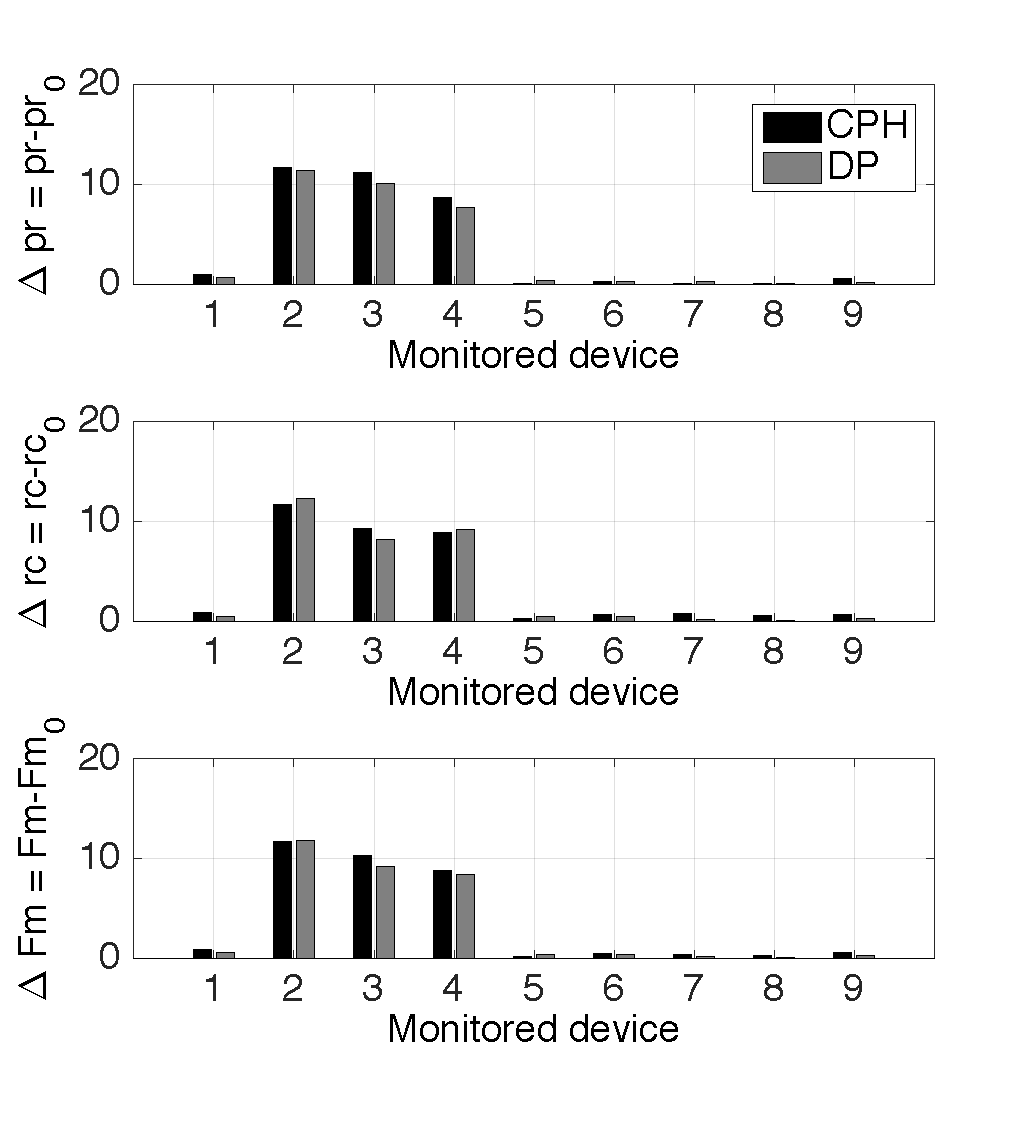
\includegraphics[width=7cm]{./chapters/chapter5/images/R1_kp_1modev.pdf}}
%  \vspace{1.5cm}
  \centerline{(a) REDD 1}\medskip
\end{minipage}
\hfill
\begin{minipage}[b]{.48\linewidth}
  \centering
  \centerline{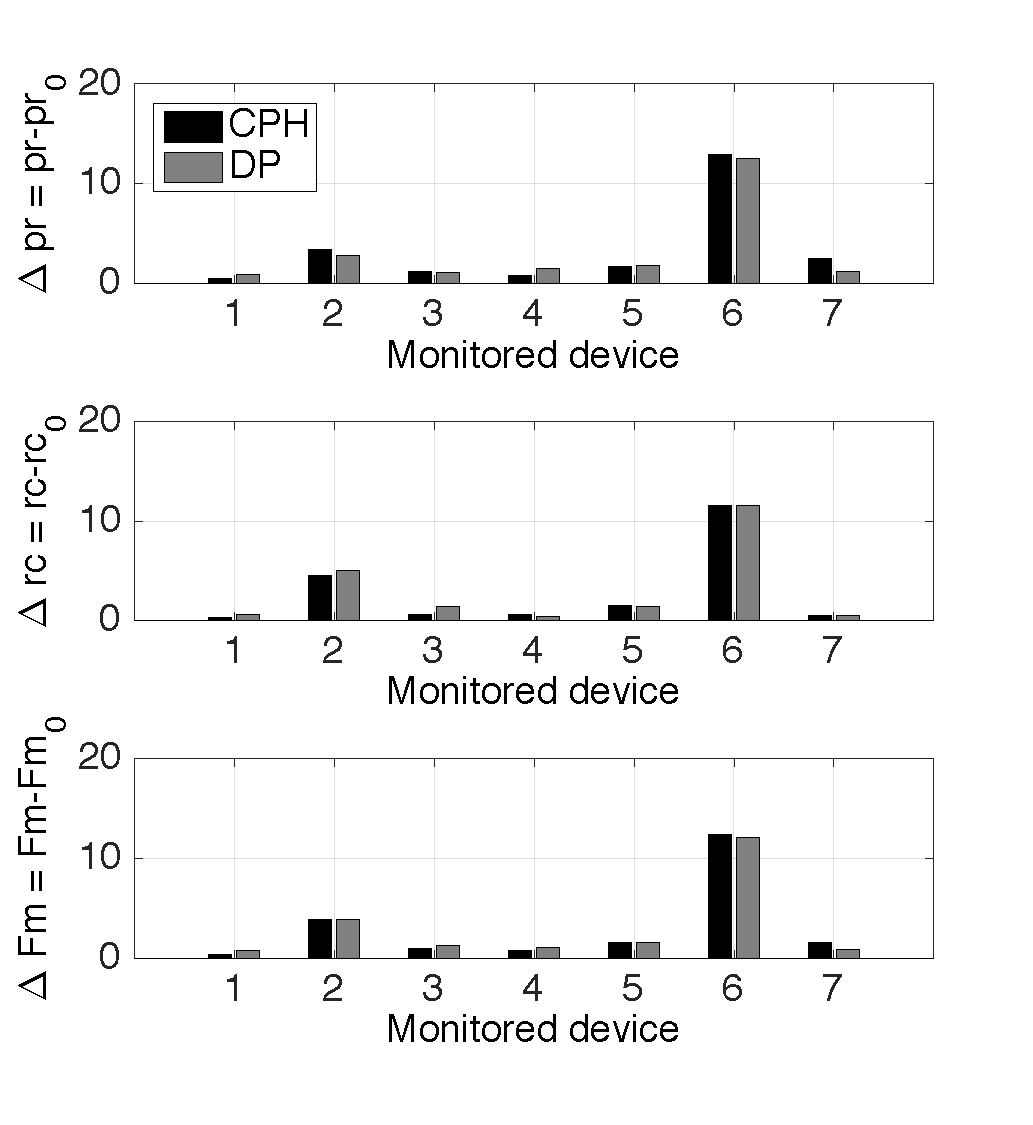
\includegraphics[width=7cm]{./chapters/chapter5/images/R2_kp_1modev.pdf}}
%  \vspace{1.5cm}
  \centerline{(b) REDD 2}\medskip
\end{minipage}
\begin{minipage}[b]{.48\linewidth}
  \centering
  \centerline{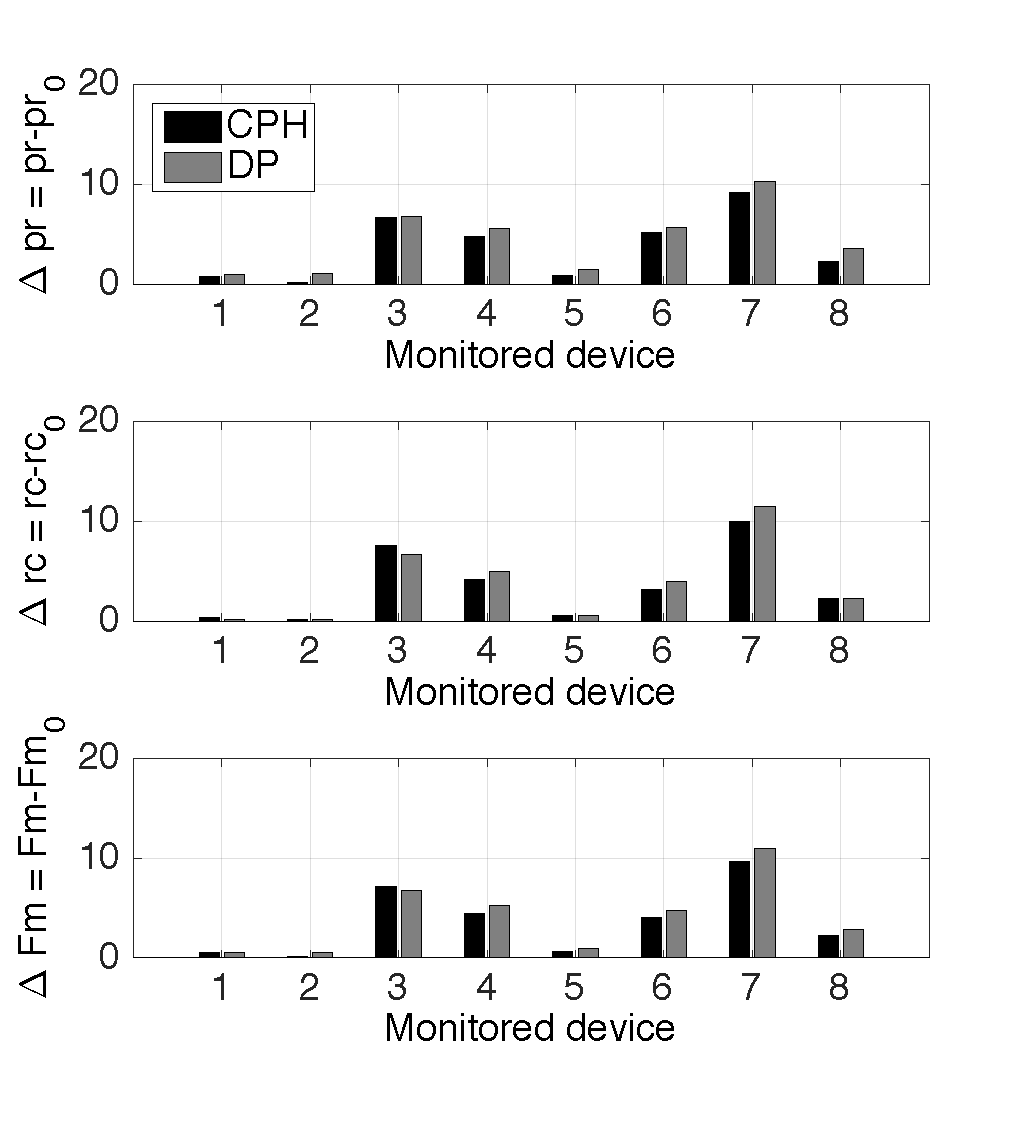
\includegraphics[width=7cm]{./chapters/chapter5/images/UK_kp_1modev.pdf}}
%  \vspace{1.5cm}
  \centerline{(c) UK-DALE 5}\medskip
\end{minipage}
\hfill
\begin{minipage}[b]{0.48\linewidth}
  \centering
  \centerline{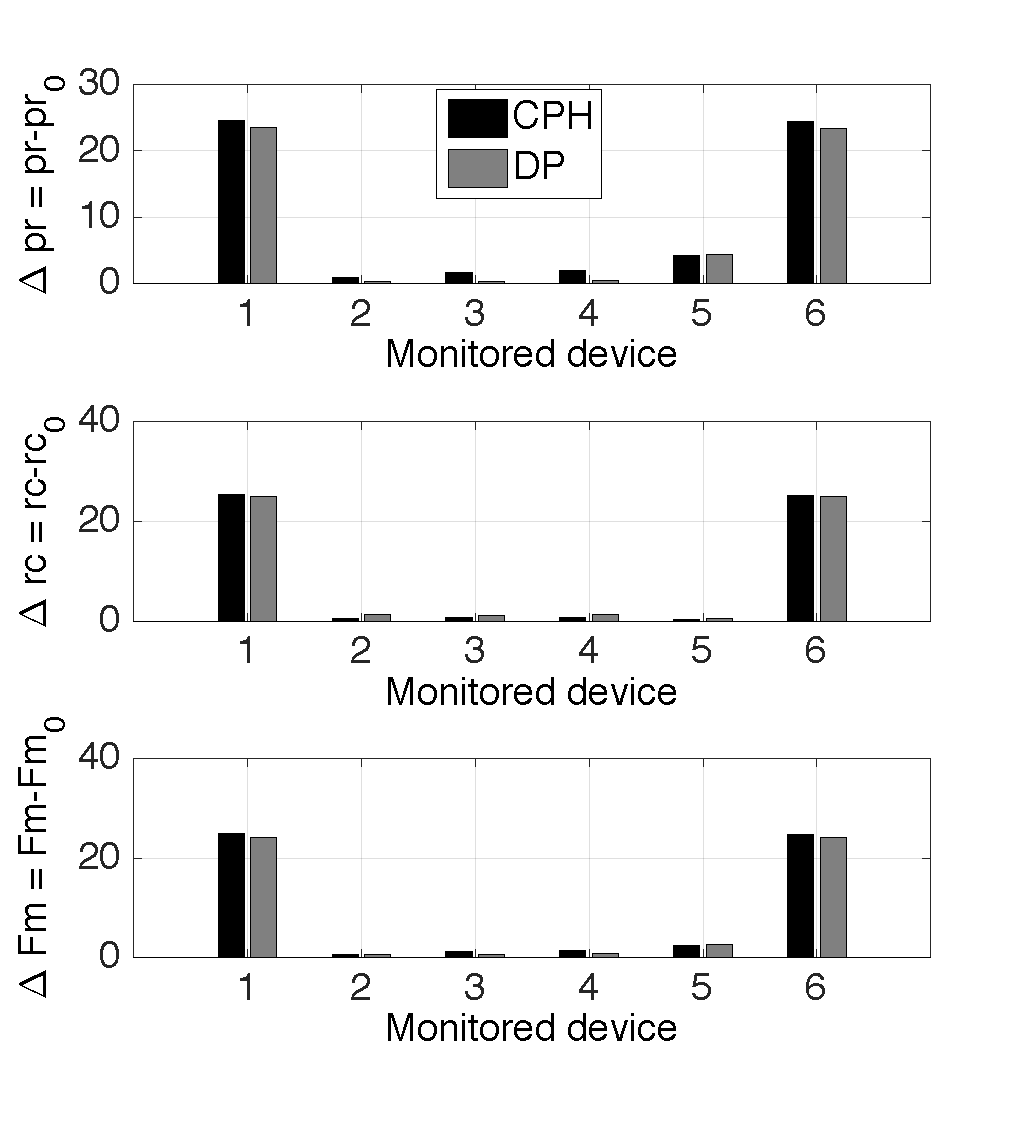
\includegraphics[width=7cm]{./chapters/chapter5/images/A_kp_1modev.pdf}}
%  \vspace{1.5cm}
  \centerline{(d) Athemium}\medskip
\end{minipage}
\caption{Effect of the type of monitored devices on the performance improvement of the CPH and DP algorithms. The values of $pr_0$, $rc_0$, $Fm_0$ correspond to the case without any monitored device, given in Table~\ref{table:SR6}.}
\label{fig:SR1}
%
\end{figure}

\subsection{Implementation results of Optical Network Interface}

In SmartSense, only several specific devices are selected to be monitored, but a relevant question is: Which type of devices can help to improve the performance of the algorithms? In the first experiment, sequentially each device is selected to monitor, the main characteristics of the devices giving the best performance are then analyzed to generalize the criteria to select the monitored devices. 
The precision and recall of the sensors detection are assumed to be equal to $0.9$. Figure~\ref{fig:SR1} shows the performance of the CPH and DP algorithms with different monitored devices in four dataset, in which the labels are respectively noted in Tables \ref{table:SR1}, \ref{table:SR2}, \ref{table:SR3} and \ref{table:SR4}. Because both CPH and DP are searching for the optimal solution, they give similar results.
Table~\ref{table:SR7} lists two devices with the best performance in each dataset. 
In REDD~1, as shown in Figure~\ref{fig:SR1}(a), the best performance corresponds to the fridge with the gain of both precision and recall around 12$\%$. From Table~\ref{table:SR1}, it can be seen that the fridge has a high using rate (24.94$\%$) and its power demand is confused with the dish washer (193W \emph{vs.} 214W). Two other devices also giving a high gain are the dish washer and the lighting system. The lighting system has the largest using rate (48.99$\%$). Although unusually operating, monitoring the dish washer also gives a high performance gain because it consumes a power similar to the fridge. Meanwhile, other devices show a very small gain (<2$\%$) if monitored.
In Figure~\ref{fig:SR1}(b), except for the fridge with the performance improvement over 12$\%$ for all evaluation metrics, deploying the sensors to monitor other devices in REDD~2 can only obtain a gain lower than 5$\%$. This result can be explained from Table~\ref{table:SR2} that besides the most used device (44.40$\%$), the fridge consumes a power very close to the lighting system (163W \emph{vs.} 153W) and stove (426W \emph{vs.} 406W). 
\par Therefore, we can come to a conclusion that the most effective devices to be monitored with CPH and DP algorithms have two main characteristics that are: high using rate and confusion on the power demand with other devices. This conclusion is also consolidated by the results from the UK-DALE~5 and Athemium dataset. As shown in Figure~\ref{fig:SR1}(c), the most effective devices in UK-DALE~5 are the microwave and fridge, which both have high using ratio (68.4$\%$ and 36.48$\%$ respectively) and their power demand is also confused with others. Concretely, the microwave consumes a power close to the washer dryer (1496W and 1492W) and dish washer (49.8W and 57.4W), while the power demand of the fridge is near to the dish washer (109.5W and 96.3W). Meanwhile, in Figure~\ref{fig:SR1}(d), the most effective devices in Athemium dataset are fridge and monitor, which are frequently used (17.79$\%$ and 27.35$\%$ respectively) and their power consumption is also similar (75W and 73W).

\begin{table}
\caption{Most effective devices with the CPH and DP algorithms.}\label{table:SR7}
\begin{center}
\begin{tabular}{|c|c|c|}
\hline
 & CPH & DP \\
 \hline
  \multirow{2}{*}{REDD 1} &2-fridge & 2-fridge \\
 & 3-dish washer & 3-dish washer  \\
 \hline
  \multirow{2}{*}{REDD 2} & 6-fridge & 6-fridge \\
 & 2-lighting & 2-lighting  \\
 \hline
  \multirow{2}{*}{UK-DALE 5} & 7-microwave & 7-microwave\\
  & 3-fridge &3-fridge \\
 \hline
  \multirow{2}{*}{Athemium} & 1-fridge & 1-fridge  \\
 & 6-monitor & 6-monitor  \\
 \hline
\end{tabular}
\end{center}
\end{table}

\begin{figure}[htb]
\begin{minipage}[b]{0.48\linewidth}
  \centering
  \centerline{\includegraphics[width=7cm]{./chapters/chapter5/images/R1_kp_nmodev.pdf}}
%  \vspace{1.5cm}
  \centerline{(a) REDD 1}\medskip
\end{minipage}
%
\hfill
\begin{minipage}[b]{.48\linewidth}
  \centering
  \centerline{\includegraphics[width=7cm]{./chapters/chapter5/images/R2_kp_nmodev.pdf}}
%  \vspace{1.5cm}
  \centerline{(b) REDD 2}\medskip
\end{minipage}
\begin{minipage}[b]{.48\linewidth}
  \centering
  \centerline{\includegraphics[width=7cm]{./chapters/chapter5/images/UK_kp_nmodev.pdf}}
%  \vspace{1.5cm}
  \centerline{(c) UK-DALE 5}\medskip
\end{minipage}
\hfill
\begin{minipage}[b]{0.48\linewidth}
  \centering
  \centerline{\includegraphics[width=7cm]{./chapters/chapter5/images/A_kp_nmodev.pdf}}
%  \vspace{1.5cm}
  \centerline{(d) Athemium}\medskip
\end{minipage}
\caption{Effect of the number of monitored devices on the performance improvement of the CPH and DP algorithms. The values of $pr_0$, $rc_0$, $Fm_0$ correspond to the case without any monitored device, given in Table~\ref{table:SR6}.}
\label{fig:SR2}
%
\end{figure}

Besides the type, the number of monitored devices is also a parameter strongly affecting on the performance improvement of the algorithms. Apparently, monitoring more devices allows to obtain a better performance. However, the deployment cost also increases along with the size of the monitoring sensors network and the non-intrusive requirement is violated. Therefore, it is necessary to make a trade-off between the size of the WSN and the desired performance when selecting the monitored devices. Figure~\ref{fig:SR2} shows the performance improvement when increasing the number of monitored devices. In each case, the devices are selected based on their performance in Figure~\ref{fig:SR1}. Obviously, there are some devices showing less effectiveness when monitored and adding them to the monitoring list cannot help to significantly improve the performance. Thus, these devices can be ignored when deploying the sensors network. 
Concretely, in REDD~1, three devices giving the best performance are fridge, dish washer and lighting system. Thus, adding these devices to the monitoring list allows to significantly improve the performance of the algorithms. This phenomenon can be illustrated by the slope from one to three devices in Figure~\ref{fig:SR2}(a). The corresponding precision gain increases from 12$\%$ to 30$\%$ and the recall from 11$\%$ to 19$\%$ in this interval. However, other devices are less effective, which results in a slow increase of the performance gain with more than three monitored devices (from 30$\%$ to 37$\%$ with precision and 19$\%$ to 23$\%$ with recall when increasing the number of devices from three to nine).
Similarly, in REDD~2, as shown in Figure~\ref{fig:SR2}(b), the performance is improved very slowly. After monitoring the first device (fridge) and obtaining the precision gain of 13$\%$ and recall gain of 12$\%$, we can only improve the recall around 3$\%$ (from 12$\%$ to 15$\%$) with other six devices added to the monitoring list. Therefore, the F-measure is still insignificant (11$\%$ improved) although the precision gain can be improved from 13$\%$ up to 31$\%$.
Meanwhile, in UK-DALE~5, there are two devices giving a remarkable increase of the performance when monitored including the microwave and fridge, as shown in Figure~\ref{fig:SR1}(c). This is the reason why the performance is significantly improved with the number of monitored devices from one to two, and slowly increased with more other devices.
In contrast, in Athemium dataset, because the fridge and the monitor have only one power state and their power demand are confused together, the performance can be significantly improved by monitoring one of them and it cannot increase anymore if another remaining device is also monitored. This results in the nearly horizontal line from one to two devices in Figure~\ref{fig:SR2}(d). Besides, the performance gain cannot be improved too much when monitoring more other devices.


\begin{figure}[htb]
\begin{minipage}[b]{1\linewidth}
  \centering
  \centerline{\includegraphics[width=0.75\textwidth]{./chapters/chapter5/images/R1_cph_pr.pdf}}
%  \vspace{1.5cm}
  \centerline{(a) REDD 1}\medskip
\end{minipage}
\hfill
\begin{minipage}[b]{1\linewidth}
  \centering
  \centerline{\includegraphics[width=0.75\textwidth]{./chapters/chapter5/images/R2_cph_pr.pdf}}
%  \vspace{1.5cm}
  \centerline{(b) REDD 2}\medskip
\end{minipage}
\caption{Performance improvement of the CPH algorithm when modifying WSN precision.}
\label{fig:SR3}
%
\end{figure}


\begin{figure}[h]
\centering
\includegraphics[width=0.65\textwidth]{./chapters/chapter5/images/breakPR.pdf} 
\caption{Dependence of the abnormally changing point on the number of states.} 
\label{fig:SR4} 
\end{figure}







\subsubsection{ECC codecs implementation}

In the experiments above, the WSN is assumed with a detection reliability of $0.9$. However, in real condition, this value can vary depending on the quality of the sensors. Therefore, we will consider the effect of the sensor detection on the overall performance of SmartSense algorithms by tuning the precision from 0.6 to 0.9 with two monitored devices (fridge and dish washer) for REDD~1 and REDD~2. Figure~\ref{fig:SR3} shows the performance gain of the CPH algorithm according to the increase of the WSN precision. 
In Figure~\ref{fig:SR3}(a), with monitored devices, the performance of the algorithm in REDD~1 decreases significantly if the reliability of the sensors is lower than 0.66. This is illustrated by the negative gain of both precision and recall. Meanwhile, when increasing this value from 0.66 to 0.68, the performance abnormally increases with the precision gain from 9$\%$ to 16.5$\%$ and the recall from 1$\%$ to 9$\%$. After this interval, the performance is slowly improved to 20$\%$ of precision gain and 15$\%$ of recall gain at a WSN precision of 0.9.
Similarly, with REDD~2, as shown in Figure~\ref{fig:SR3}(b), the performance gain is also negative with the WSN reliability less than 0.6 and there also exists an abnormally changing interval between 0.66 and 0.68, in which the precision gain increases from -7.5$\%$ to 12.5$\%$ and the recall from -12$\%$ to 8$\%$. Beyond this interval, the performance slowly increases along with the WSN precision.
To find the reason of the abnormally increasing interval, let return to Section~\ref{knapsack}. If an $m$-state device is detected as switched on, the corresponding probability of each power state is equal to $pr/m$ and off-state is $(1-pr)$. Thus, with $pr<m/(m+1)$, the probability of the off-state is greater than any on-state although the device is operating and that makes the decrease of performance. In contrast, if $pr>m/(m+1)$, the probability of any on-state is larger than off-state and the probability information allows to improve the detection accuracy. In both REDD~1 and REDD~2 dataset, the monitored devices are fridge and dish washer, each of which has two operation states, which creates a changing point at $pr\approx 0.67$. Obviously, with the edge detector approach, this phenomenon always happens at $pr = 0.5$. 
The dependence of the changing point $pr=\frac{m}{m+1}$ on the number of states of devices is presented in Figure~\ref{fig:SR4}. \par As a consequence, the reliability of the WSN needs to ensure to stay on the upper plane discriminated by the changing curve in order to allow the algorithm to reach a better performance. 










\begin{figure}[htb]
\begin{minipage}[b]{0.48\linewidth}
  \centering
  \centerline{\includegraphics[width=7cm]{./chapters/chapter5/images/R1_ed_1modev.pdf}}
%  \vspace{1.5cm}
  \centerline{(a) REDD 1}\medskip
\end{minipage}
%
\hfill
\begin{minipage}[b]{.48\linewidth}
  \centering
  \centerline{\includegraphics[width=7cm]{./chapters/chapter5/images/R2_ed_1modev.pdf}}
%  \vspace{1.5cm}
  \centerline{(b) REDD 2}\medskip
\end{minipage}

\caption{Effect of the type of monitored devices on the performance improvement of the DTW and ED algorithms. The values of $pr_0$, $rc_0$, $Fm_0$ correspond to the case without any monitored device, given in Table~\ref{table:SR6}.}
\label{fig:SR5}
%
\end{figure}



\subsubsection{Serializer -- Deserializer implementation}

Similar to CPH and DP algorithms, the performance of the DTW and ED algorithms in SmartSense also depends on the type of monitored devices. To analyze the main characteristics of the most effective devices, each device in REDD~1 and REDD~2 is sequentially selected to monitored. The performance gain compared with the original algorithms in NILM, given in Table~\ref{table:SR6}, is shown in Figure~\ref{fig:SR5}. Two devices in each dataset giving the best gain are listed in Table~\ref{table:SR8}.
As shown in Figure~\ref{fig:SR5}(a), the fridge is the best effective device to be monitored in REDD~1. By applying the ED algorithm, monitoring the fridge can achieve a precision gain of 4$\%$ and recall gain of 4.2$\%$. Comparing with Table~\ref{table:SR2}, because the fridge has the confusion on the power demand with the dish washer, both devices have a near value of edge height, which reduces the performance of the edge detector based algorithms in a traditional NILM system. By monitoring one of them, the ambiguity can be overcome. Besides, the fridge also has a high number of activations during the observation period (1695 times). Obviously, monitoring the devices with high number of uses allows to increase the overall performance of the algorithms. The second largest gain in REDD~1 corresponds to the dish washer with 3$\%$ and 2$\%$ for the gain of precision and recall, respectively. Besides confused with the fridge on the edges height, this device is also frequently switched on/off. 
Meanwhile, the performance improvement given by the DTW algorithm is lower then the ED one with only 2$\%$ of precision gain and 1.4$\%$ of recall gain when monitoring the fridge. The respective results for the dish washer are 1.9$\%$ and 0.25$\%$. The small gain of the DTW algorithm with this dataset can be explained by the fact that it shows a good performance without any monitored device ($pr=83.53\%$, $rc=76.48\%$) and it is difficult to improve its performance.
In REDD~2, as shown in Figure~\ref{fig:SR5}(b), the best gain also corresponds to the fridge with 3.9$\%$ of precision and 6.9$\%$ of recall with ED algorithm. The respective values with DTW method are 4.05$\%$ and 3.9$\%$. Similar to REDD~1, the fridge in REDD~2 is also the most frequently used device and its edges are also ambiguous with the lighting system (153W) and dish washer (426W) when it changes the state from 163W to 426W with a rising edge of 263W. This is also the reason why the dish washer is the second effective device in this dataset.
From the results in Figure~\ref{fig:SR5}, it can be concluded that the edge detector based algorithms are sensible with the devices more frequently switched on/off and having the confusion on the edges height (correlated to the power demand) with the others. Therefore, it is necessary to analyze these two characteristics to select the effective monitored devices.

\begin{figure}[htb]

\begin{minipage}[b]{0.48\linewidth}
  \centering
  \centerline{\includegraphics[width=7cm]{./chapters/chapter5/images/R1_ed_nmodev.pdf}}
%  \vspace{1.5cm}
  \centerline{(a) REDD 1}\medskip
\end{minipage}
%
\hfill
\begin{minipage}[b]{.48\linewidth}
  \centering
  \centerline{\includegraphics[width=7cm]{./chapters/chapter5/images/R2_ed_nmodev.pdf}}
%  \vspace{1.5cm}
  \centerline{(b) REDD 2}\medskip
\end{minipage}
\caption{Effect of the number of monitored devices on the performance improvement of the DTW and ED algorithms. The values of $pr_0$, $rc_0$, $Fm_0$ correspond to the case without any monitored device, given in Table~\ref{table:SR6}.}
\label{fig:SR6}
%
\end{figure}


\begin{table}
\caption{Most effective devices with DTW and ED algorithms.}\label{table:SR8}
\begin{center}
\begin{tabular}{|c|c|c|}
\hline
& DTW & ED\\
\hline
\multirow{2}{*}{REDD 1} & 2-fridge &2-fridge \\
& 3-dish washer & 3-dish washer \\
\hline
\multirow{2}{*}{REDD 2}  & 6-fridge&6-fridge \\
& 7-dish washer&7-dish washer \\
\hline
\end{tabular}
\end{center}
\end{table}
\subsubsection{Allocator implementation}
The performance gain also slowly increases when adding more devices to the monitoring list, as illustrated in Figure~\ref{fig:SR6}. In this results, the monitored devices are selected based on their performance in Figure~\ref{fig:SR5}. In Figure~\ref{fig:SR6}(a), with two monitored devices (fridge and dish washer) in REDD~1, the precision of the ED algorithm can be improved by 6$\%$ and the recall by 5$\%$. Meanwhile, with other additional devices, the precision can only increase by 2.8$\%$ (from 6$\%$ to 8.8$\%$) and the recall by 1.5$\%$ (from 5$\%$ to 6.5$\%$). Similarly, in REDD~2 as shown in Figure~\ref{fig:SR6}(b), the performance gain obtainable with the ED algorithm is 5$\%$ of precision and 8.5$\%$ of recall with only fridge and dish washer monitored. Then, it increases very slowly when adding more devices to the monitoring list. Concretely, the precision gain increases from 5$\%$ to 6.5$\%$ and the recall from 8.5$\%$ to 9$\%$ with the number of devices from two to seven. Therefore, it is necessary to evaluate the efficiency of each device in improving the overall performance before deploying the monitoring sensors.

\begin{figure}[htb]
\begin{minipage}[b]{1\linewidth}
  \centering
  \centerline{\includegraphics[width=0.75\textwidth]{./chapters/chapter5/images/R1_ed_pr.pdf}}
%  \vspace{1.5cm}
  \centerline{(a) REDD 1}\medskip
\end{minipage}
\hfill
\begin{minipage}[b]{1\linewidth}
  \centering
  \centerline{\includegraphics[width=0.75\textwidth]{./chapters/chapter5/images/R2_ed_pr.pdf}}
%  \vspace{1.5cm}
  \centerline{(b) REDD 2}\medskip
\end{minipage}
\caption{Performance improvement of the ED algorithm versus the WSN precision.}
\label{fig:SR7}
%
\end{figure}

Similar to CPH and DP, the performance of the edge detector based algorithms also increases along with the increase of the WSN detection precision, as illustrated by the simulation results of ED one with REDD~1 and REDD~2 in Figure~\ref{fig:SR7}. Because the operating probability of each device is not divided by the number of states, there is only one abnormally changing point at $pr=0.5$ for these algorithms. This point is not presented in Figure~\ref{fig:SR7} because the value of WSN precision is only tuned from 0.6 to 0.9. Moreover, a WSN precision of 0.5 is equivalent to a random selection of the state, which is not relevant in our case.





\subsection{Communication time and latency}
\begin{figure}[htb]

\begin{minipage}[b]{1\linewidth}
  \centering
  \centerline{\includegraphics[width=.75\textwidth]{./chapters/chapter5/images/R1_perfcom.pdf}}
%  \vspace{1.5cm}
  \centerline{(a) REDD 1}\medskip
\end{minipage}
%
\hfill
\begin{minipage}[b]{1\linewidth}
  \centering
  \centerline{\includegraphics[width=.75\textwidth]{./chapters/chapter5/images/R2_perfcom.pdf}}
%  \vspace{1.5cm}
  \centerline{(b) REDD 2}\medskip
\end{minipage}
\caption{Performance comparison of the proposed algorithms with two monitored devices.}
\label{fig:SR8}
%
\end{figure}

Comparing with the CPH and DP methods, it can be noticed that the improvement of the DTW and ED algorithms is much lower. As presented in Table~\ref{table:SR6}, these algorithms show high performance without monitored device. Concretely, the F-measure of the ED algorithm is greater than 75$\%$ and the DTW one over 79$\%$. Meanwhile, the CPH and DP algorithms can only show an F-measure lower than 70$\%$. Obviously, high performance prevents the edge detector based algorithms from giving a high gain. In addition, the results also come from the fact that performance of these algorithms also depends on the edge detector capacity. Therefore, despite outperforming the algorithms with the knapsack approach in a traditional NILM system, both DTW and ED algorithms can only show a near performance in term of F-measure with two monitored devices, as illustrated in Figure~\ref{fig:SR8}. Of course, comparing the increase of the gain in Figures~\ref{fig:SR2} and \ref{fig:SR6}, the CPH and DP algorithms can show a better performance than the ED and DTW ones with more than two monitored devices in home.
Besides the overall performance, the performance per device of each proposed algorithms with two monitored devices for each dataset (selected by the results in Figure~\ref{fig:SR1} for CPH and DP algorithms and Figure~\ref{fig:SR5} for ED and DTW ones) is also presented in Tables~\ref{table:SR9}, \ref{table:SR10}, \ref{table:SR11} and \ref{table:SR12}, respectively.

\begin{table}
\caption{Performance per device in REDD~1 ($\%$).}\label{table:SR9}
\begin{center}
\begin{tabular}{|c|c|c|c|c|c|c|c|c|c|c|}
\hline
\multicolumn{2}{|c|}{Device}& 1&2&3&4&5&6&7&8&9\\
\hline
\multirow{3}{*}{CPH} & $pr$ &65.08 &97.66 &86.64 &78.55 &41.69 &19.23 &22.77 &30.14 &97.16 \\
& $rc$ & 36.80&88.95 &87.66 &79.28 &46.53 &45.17 &35.11 &29.46 &69.22  \\
& $Fm$ &47.01 &93.10 &87.15 &78.91 &43.97 &26.98 &27.63 &29.79 &80.84 \\
\hline
\multirow{3}{*}{DP} & $pr$ & 63.94&99.16 &96.50 &76.55 &43.79 &22.50 &20.63 &19.91 &94.68 \\
& $rc$ &35.84 &91.59 &92.13 &76.00 &41.20 &46.26 &42.84 &25.71 &73.34  \\
& $Fm$ &45.93 &95.23 &94.26 &76.27 &42.45 &30.28 &27.85 &22.44 &82.66 \\
\hline
\multirow{3}{*}{ED} & $pr$ &42.88 &93.65 &95.81 &61.91 &31.33 &40.52 &49.27 &21.17 &99.75 \\
& $rc$ &59.66 &80.43 &83.88 &61.35 &68.01 &61.91 &43.21 &19.12 &54.18  \\
& $Fm$ &49.89 & 86.54 & 89.45 & 61.63 &42.90 & 48.98 &46.04 & 20.09 & 70.72 \\
\hline
\multirow{3}{*}{DTW} & $pr$ &47.54 &89.35 &80.85 &68.81 &34.17 &87.41 &94.36 &21.46 &99.36 \\
& $rc$ &74.95 &85.90 &86.19 & 25.05&68.01 &65.17 &60.77 &20.45 &67.61  \\
& $Fm$ &58.18 &87.59 &83.43 &36.73 &45.48 &74.67 &73.93 &20.94 &40.47 \\
\hline
\end{tabular}
\end{center}
\end{table}

\begin{table}
\caption{Performance per device in REDD~2 ($\%$).}\label{table:SR10}
\begin{center}
\begin{tabular}{|c|c|c|c|c|c|c|c|c|}
\hline
\multicolumn{2}{|c|}{Device}& 1&2&3&4&5&6&7\\
\hline
\multirow{3}{*}{CPH} & $pr$ &23.10 &91.60 &27.17 &99.25 &62.23 &99.92 &27.42  \\
& $rc$ & 24.20& 86.62&85.80 &30.73 &56.47 &92.86 &55.58  \\
& $Fm$ & 23.64&89.04 &41.27 &46.94 &59.21 &96.26 &36.72  \\
\hline
\multirow{3}{*}{DP} & $pr$ & 27.18&95.53 &26.02 &97.33 &48.57 &99.95 &26.82 \\
& $rc$ & 43.19&90.49 &86.80 &21.84 &38.09 &88.44 &57.10   \\
& $Fm$ &33.36 &92.94 &40.04 &35.67 &42.70 &93.85 &36.50  \\
\hline
\multirow{3}{*}{ED} & $pr$ & 80.65 &94.05 &21.55 &100 & 63.09 &85.60 &82.71\\
& $rc$ &19.65 & 41.75 & 99.13 & 17.62 & 85.12 & 85.96 & 84.43   \\
& $Fm$ & 31.60 & 57.82 & 35.40 & 29.96 & 72.47 & 85.78 & 83.56  \\
\hline
\multirow{3}{*}{DTW} & $pr$ & 81.56& 95.07 &21.55 & 52.71& 63.09&84.37&80.54 \\
& $rc$ & 29.46&43.19 &93.13 &39.64 &85.12 &90.27 &83.92  \\
& $Fm$ &43.29 &59.40 &35.01 &45.62 &72.47 &87.22 &82.19  \\
\hline
\end{tabular}
\end{center}
\end{table}

\begin{table}
\caption{Performance per device in UK-DALE~5 ($\%$).}\label{table:SR11}
\begin{center}
\begin{tabular}{|c|c|c|c|c|c|c|c|c|c|}
\hline
\multicolumn{2}{|c|}{Device}& 1&2&3&4&5&6&7&8\\
\hline
\multirow{3}{*}{CPH} & $pr$ &22.83 &36.99 &91.24 &40.35 & 17.48 &22.15 &97.46 &87.10 \\
& $rc$ &69.10 &55.31 &89.88 &24.74 &52.20 &67.68 &85.72 &75.84  \\
& $Fm$ &34.32 &44.33 &90.55 &30.67 &26.19 &33.38 &91.21 &81.08 \\
\hline
\multirow{3}{*}{DP} & $pr$ &23.57 &40.77 &90.57 &37.47 &25.81 &23.08 &98.31 &88.52 \\
& $rc$ &58.02 &80.19 &89.15 &22.66 &53.18 &72.60 &87.45 &65.03  \\
& $Fm$ & 33.52&54.08 &89.86 &28.24 &34.75 &35.02 &92.56 &74.98 \\
\hline
\end{tabular}
\end{center}
\end{table}

\begin{table}
\caption{Performance per device in Athemium dataset ($\%$).}\label{table:SR12}
\begin{center}
\begin{tabular}{|c|c|c|c|c|c|c|c|c|c|}
\hline
\multicolumn{2}{|c|}{Device}& 1&2&3&4&5&6\\
\hline
\multirow{3}{*}{CPH} & $pr$ & 93.55 & 86.17& 98.91 &65.31 &85.73 &99.16 \\
& $rc$ &99.14 &99.16 &81.69 &80.41 &98.61 &95.01  \\
& $Fm$ &96.27 &92.21 &89.48 &72.08 &91.72 &97.04  \\
\hline
\multirow{3}{*}{DP} & $pr$ & 86.43 &89.73 &100 &65.60 &82.63 &99.41 \\
& $rc$ & 99.46&99.16 &91.09 &87.80 &98.89 &87.92   \\
& $Fm$ & 92.49&94.21 &95.34 &75.09 &90.03 &93.31 \\
\hline
\end{tabular}
\end{center}
\end{table}

Apparently, the detection of the monitored devices is significantly improved.  For example in REDD~1, as in Table~\ref{table:SR9}, both fridge (2) and dish washer (3) are identified with the precision and recall greater than 85$\%$ by the CPH and DP algorithms and over 80$\%$ by the edge detector ones. Concretely, without sensors, the performance of the CPH algorithm with the fridge is only 62.13$\%$ of precision and 57.78$\%$ of recall as shown in Table~\ref{table:SR6a}, but they are significantly improved up to 97.66$\%$ and 88.95$\%$, respectively, in SmartSense. Similarly, the reliability of detecting the dish washer also increases from 23.83$\%$ to 81.64$\%$ and the sensibility increases from 69.28$\%$ to 87.66$\%$. Meanwhile, the precision of the DTW approach increases from 85.39$\%$ to 89.35$\%$ when detecting the fridge and from 78.85$\%$ to 80.85$\%$ when detecting the dish washer. The respective recall is from 83.49$\%$ to 85.9$\%$ and from 56.19$\%$ to 86.19$\%$. The performance improvement of the monitored devices in other dataset is similar.
In SmartSense, not only the detection of the monitored devices but the identification of other loads is also improved. It comes from the fact that in each dataset, these loads have confusions on the power demand with the monitored ones and the additional information in SmartSense helps to overcome this ambiguity.
For example in REDD~2, referring to Tables~\ref{table:SR6b} and \ref{table:SR10}, the performance of the DTW algorithm when detecting the lighting system can be improved from 94.17$\%$ to 95.07$\%$ with precision and from 39.01$\%$ to 43.19$\%$ with recall because the fridge, which has one power state ambiguous with the lighting, is monitored by the sensors. Therefore, by monitoring only a subset of all devices, the overall performance of the NILM algorithms can be improved using the SmartSense approach.




\subsection{Complexity of synchronization analysis}
% complexity
Algorithmic complexity, expressed through the number of multiplications and additions to process each dataset, is given in Table~\ref{table:SR13} for the proposed algorithms. These parameters do not depend on the number of monitored devices. Apparently, the CPH algorithm is the most complex because it requires a large number of multiplications and additions to calculate the elements of each tuple. 
\begin{table}
\caption{Number of computations.}\label{table:SR13}
\begin{center}
\begin{tabular}{|c|c|c|c|c|}
\hline
 & \multicolumn{2}{c|}{REDD 1}&\multicolumn{2}{c|}{REDD 2}\\
\hline
 & Multiplications & Additions&Multiplications & Additions\\
 \hline
 CPH & $3.36\times 10^5$ & $3.64\times 10^7$& $1.10\times 10^5$&$9.20\times 10^6$\\
 \hline
 DP & $1.27\times 10^5 $&$3.69\times 10^7$&$6.69\times 10^4$ & $3.60\times 10^6$\\
 \hline
 ED& $3.14\times 10^3$ & $1.68\times 10^5$& $2.45 \times 10^3$&$1.05 \times 10^5$\\
 \hline
 DTW  & $4.60\times 10^3$ & $1.47\times 10^7$&$3.71\times 10^3$&$3.80\times 10^6$\\
 \hline
 \multicolumn{5}{|c|}{ }\\
 \hline
  &\multicolumn{2}{c|}{UK-DALE 5}& \multicolumn{2}{c|}{Athemium}\\
\hline
 & Multiplications & Additions&Multiplications & Additions\\
 \hline
 CPH & $7.93\times 10^6$ & $9.21\times 10^8$ & $1.02\times 10^5$ & $6.53\times 10^6$  \\
 \hline
 DP  & $1.55\times 10^6$& $3.58\times 10^8$ & $7.62\times 10^4$ & $2.94\times 10^6$  \\
 \hline
\end{tabular}
\end{center}
\end{table}
From Section~\ref{CPH}, the CPH algorithm has an exponential complexity in the worst case. If each device has $m$ states and if all possible combinations are Pareto points, there are $m^N$ tuples after the last iteration and the Pareto minimization process has the complexity of $m^{2N}$. Nevertheless, if only $L$ solutions are retained instead of all Pareto points at each iteration, there are only $L^2$ tuples appearing after combining two input sets. Hence, an $L^4$-complex process is necessary to search for the Pareto points and that results in a complexity of $NL^4$ for the CPH algorithm. The selection of $L$ best tuples can be executed as in~\cite{Shojaei13}. Denote $r = d_1$ and $v = -d_3$, the Pareto points satisfy the following characteristic:
\begin{eqnarray}
\forall i,j: v_i \leq v_j \leftrightarrow r_i \leq r_j.
\end{eqnarray}
At first, two Pareto points $(r_{\max},v_{\max})$ and $(r_{\min},v_{\min})$ are selected, which results in two constant product values $c_{\max} = v_{\max}\times r_{\max}$ and $c_{\min} = v_{\min}\times r_{\min}$. To select the $(L-2)$ remaining points, the range $c_{\min}..c_{\max}$ will be divided into $(L-1)$ parts equally discriminated by $(L-2)$ boundary points $c$. For each of $(L-2)$ values $c$, a Pareto point giving the product of $v\times r$ closest to $c$ will be kept. 
The decrease of $L$ allows to reduce the computational complexity. However, this increases the risk of rejecting the true combination from the final set of tuples and the decrease of the load disaggregation performance, as illustrated in Figure~\ref{fig:SR9}. 
In Figure~\ref{fig:SR9}(a), with two monitored devices in REDD~1, the performance gain can be obtained with 20$\%$ of precision and 14.5$\%$ of recall if there are 125 partial solutions retained after each iteration. This selection of $L$ leads to a large number of multiplications ($3.36\times 10^5$) and additions ($3.64\times 10^7$) to execute the dataset. By reducing the value of $L$, the number of computations can significantly decrease, e.g. $1.81\times 10^5$ of multiplications and $4.06\times 10^6$ of additions with $L=25$. However, the performance of the CPH algorithm also simultaneously decreases down to 17.5$\%$ of precision gain and 12$\%$ of recall gain. If keeping only 5 partial solutions, i.e. $L=5$, the number of multiplications and additions decreases to $1.37\times 10^5$ and $8.49\times 10^5$, respectively. Nevertheless, the corresponding obtainable precision and recall gain are only 15.5$\%$ and 3$\%$. 
Similarly, in REDD~2 as shown in Figure~\ref{fig:SR9}(b), the number of multiplications and additions reduce from $1.10\times 10^5$ and $9.20\times 10^6$ to $7.55\times 10^4$ and $5.18\times 10^5$, respectively, when changing the value of $L$ from 125 to 5. The performance gain also decreases from 17.5$\%$ to 12.22$\%$ and 14$\%$ to 4.5$\%$ for the precision and recall, respectively.
Therefore, driving the value of $L$ rises the need to make a trade-off between the complexity and the desired performance.
\begin{figure}[htb]
\begin{minipage}[b]{1\linewidth}
  \centering
  \centerline{\includegraphics[width=0.8\textwidth]{./chapters/chapter5/images/R1_cph_L.pdf}}
%  \vspace{1.5cm}
  \centerline{(a) REDD 1}\medskip
\end{minipage}
\hfill
\begin{minipage}[b]{1\linewidth}
  \centering
  \centerline{\includegraphics[width=0.8\textwidth]{./chapters/chapter5/images/R2_cph_L.pdf}}
%  \vspace{1.5cm}
  \centerline{(a) REDD 2}\medskip
\end{minipage}
\caption{Effect of the number of Pareto points on the performance and complexity of the CPH algorithm.}
\label{fig:SR9}
%
\end{figure}

\begin{figure}[htb]
\begin{minipage}[b]{1\linewidth}
  \centering
  \centerline{\includegraphics[width=0.8\textwidth]{./chapters/chapter5/images/R1_scale.pdf}}
%  \vspace{1.5cm}
  \centerline{(a) REDD 1}\medskip
\end{minipage}
\hfill
\begin{minipage}[b]{1\linewidth}
  \centering
  \centerline{\includegraphics[width=0.8\textwidth]{./chapters/chapter5/images/R2_scale.pdf}}
%  \vspace{1.5cm}
  \centerline{(b) REDD 2}\medskip
\end{minipage}
\caption{Effect of the scale factor on the performance and complexity of the DP algorithm.}
\label{fig:SR10}
%
\end{figure}

Similar to CPH method, the DP algorithm also needs a large amount of computations. The principle of DP is based on the construction of profit tables. Therefore, the computational complexity depends on the size of each table, correlating to the number of devices, the aggregate power and the number of computations in each cell, decided by the number of states of current device. As a consequence, the complexity reduction effort can be executed by decreasing the number of columns with a scale factor $\delta$, e.g. $w_{ij} = w_{ij}/\delta,i=1,\ldots,N,j=1,\ldots,m_i$, $R = R/\delta$. If possible, the best choice of $\delta$ is the common divisor of $R$ and $w_{ij}$. However, this condition is unrealistic and the effect of the rounding down operation makes the performance decrease, as shown in Figure~\ref{fig:SR10}.
In the DP algorithm, the construction of the profit tables is only based on the addition. This is the reason why the scale factor only affects the number of additions and does not change the number of multiplications, as illustrated in Figure~\ref{fig:SR10}(a). The results with REDD~1 in case with two monitored devices show a decrease of the number of additions from $7.35\times 10^7$ to $8.43\times 10^6$ when increasing the scale factor from 5 to 45. The performance of the algorithm also attenuates respectively by the precision gain from 24.5$\%$ to 19$\%$ and the recall gain from 15.2$\%$ to 5.5$\%$. Meanwhile, Figure~\ref{fig:SR10}(b) presents the attenuation of the performance gain from 15$\%$ to 12.7$\%$ of precision and from 12.2$\%$ to 7.2$\%$ of recall when the value of $\delta$ increases from 5 to 45 in REDD~2. This tuning also allows to significantly decrease the number of computations. Concretely, the additions reduce from $7.08\times 10^6$ to $9\times 10^5$.

Different from the algorithms in the knapsack approach, both ED and DTW are less complex. Apparently, the computational complexity of the ED algorithm depends on the number of patterns in the library. If each of the $N$ devices has $m$ patterns, the device identification procedure needs to browse $Nm$ times to find the minimum distance. Meanwhile, because taking all power values in a pattern into account, besides the number of patterns in the library, the complexity of the DTW algorithm is also decided by the length of each one. If each pattern has an average length of $l$, the accumulated distance calculation has a complexity of $l^2$, which makes the DTW become an $Nml^2$-complex algorithm. 
Despite less complexity, both ED and DTW algorithms are not suitable for the real-time application. They need to detect the falling edge before pairing with the rising one and identifying the corresponding device during this period. On the contrary, when applied to real-time energy disaggregation, the complexity of the CPH and DP one is compatible for implementation in an NILM system, since the algorithm is applied on the main system measuring the global energy consumption.

\section{Conclusions}
In this chapter, we introduce a new load monitoring system, which uses a WSN to detect and provide the operating probability of some devices to help the NILM algorithms in improving their performance. This system is called sensor-aided non-intrusive load monitoring (SmartSense). Although deploying a sensors network, SmartSense is less intrusive than other intrusive load monitoring systems such as ViridiScope~\cite{Kim09Ubicomp}, because only a subset of all devices is selected to attach with the sensors and the identification is still based on an NILM algorithm.
The operation probability is used as a feature and combined with the traditional features of NILM by a regularization parameter to create a new one. In this chapter, two approaches are proposed:
\begin{itemize}
\item Knapsack approach: the $l1$-norm minimization problem in \cite{Hart92} is modeled as a knapsack problem and solved by two proposed algorithms including compositional Pareto-algebraic heuristic, which is based on a recursive relation, and dynamic programming, based the the construction of profit tables.
\item Edge detector approach: an edge detector is applied to detect the rising edge and falling edge of an activation on the aggregate power signal and to compare them with the existing ones in the library. The rising edge and falling edge can be directly used as a feature (as in edge detection algorithm) or combined with other active power values between them (as in dynamic time warping algorithm).
\end{itemize}

By simulating all four proposed algorithms with four dataset including UK-DALE~5, REDD~1, REDD~2 and our Athemium data, the performance of the load detection can be significantly improved with some monitored devices in comparison with traditional NILM systems. To obtain a good improvement, the devices selected to be monitored need to satisfy some criteria. In the knapsack approach, selected devices are the one with high using rate and confusion on the power demand with other devices. Meanwhile, the edge detector approach needs to monitor the devices more frequently switched on/off and ambiguous with the others on the edges height.
As a consequence, only several devices in home or building are selected, satisfying these requirements and allowing to significantly improve the overall performance when monitored. The others are less effective and need to be ignored when deploying the monitoring sensor network to reduce the cost. 

Besides, comparing the performance of the proposed approaches shows that the CPH and DP algorithms outperform the ED and DTW ones with more than two monitored devices in each dataset, although in normal NILM system, they are less effective. This result comes from the fact that the performance of the ED and DTW algorithms also depends on the edge detector capacity.

However, the algorithms of the knapsack approach show a high complexity presented by the large amount of multiplications and additions. To reduce the computational complexity, we can drive some parameters such as the number of Pareto points retained after each iteration in CPH or the scale factor in DP. Nevertheless, it also causes the attenuation of the performance. 



% Chapter6

\chapter{Design exploration of thermal issue in optical network on-chip} % Write in your own chapter title
\label{l6norm}
%\addtotoc{State of the Arts}
\lhead{\emph{Algorithms for NILM based on $l1$-norm Minimization}} % Write in your own chapter title to set the page header

In this chapter, we try to solve the $l1$-norm minimization problem in Eq.~\eqref{eqI7} defined in Section~\ref{nilm} by brute force approach, also called Least Absolute Error (LAE) based algorithm. Thereby, all possible combinations of states will be sequentially tested and the most suitable one will be selected as solution. However, because of the ambiguity on power demand of different devices, many combinations can give the same or near results, which reduces the algorithm accuracy. To improve performance, we propose to apply an additional information to select the solution among all possible combinations. This is a contribution to research on NILM. Two new methods are studied and introduced in this chapter. The first one, state difference-based algorithm, uses the Hamming distance between the possible combinations and the previous state of devices to find the solution for the $l1$-norm minimization problem, as introduced in Section~\ref{diff}. Meanwhile, the second one, called state transition probability-based algorithm and introduced in Section~\ref{proba}, considers the state transition probability from previous state to current state to determine the most suitable combination. The three proposed algorithms will be simulated in Matlab with data retrieved from a set of devices in our laboratory. Simulation results will be then compared with edge detection algorithm~\cite{Hart92}.

\section{Introduction and challenges}\label{LAE}
The $l1$-norm minimization problem for Equation~\eqref{eqI7} is presented as follows:
\begin{eqnarray}\label{eqL1}
 &&\min_{\mathbf{s}}\parallel x(t)-\sum_{i=1}^{N}{\sum_{j=1}^{m_i}{s_{ij}(t)\times w_{ij}}}\parallel\\
\mbox{subject to:}&& s_{ij}(t)\in \{0,1\}, i=1,\ldots,N,j=1,\ldots,m_i\nonumber\\
&&\sum_{j=1}^{m_i}{s_{ij}(t)}\in \{0,1\}, i=1,\ldots,N. \nonumber
\end{eqnarray} 

To find the solution for problem \eqref{eqL1}, the conditions are at first processed by presenting all possible combinations of state vector $\mathbf{s}$ in matrix $\mathbf{S}$. Each row of $\mathbf{S}$ corresponds to a combination. For example, if there are two devices and each of them has two operation states, the state matrix $\mathbf{S}$ is defined as
\begin{equation*}
\mathbf{S}=\left[ \begin{array}{cccc}
0&0&0&0\\
0&0&0&1\\
0&1&0&1\\
0&1&0&0\\
0&1&1&0\\
0&0&1&0\\
1&0&1&0\\
1&0&0&0\\
1&0&0&1
\end{array}
\right]
\end{equation*}
Then, all combinations will be sequentially applied to the following equation to calculate the absolute error between the aggregate power and the total power demand of devices with corresponding state defined as
\begin{equation}\label{eqL2}
e(k) = |x(t) - \mathbf{s}^{(k)}\times \mathbf{w}^T|,
\end{equation}
where $e(k)$ is the absolute error corresponding to the combination $s^{(k)}$ in row $k$ of matrix $\mathbf{S}$. The combination giving the least value of $e(k)$ is selected as the solution. Therefore, this method is also called Least Absolute Error (LAE) based algorithm and presented in Algorithm~\ref{algoL1}. Obviously, the LAE based algorithm is exponentially complex and may be intractable with a large number of devices. However, it is considered in this chapter to study the performance improvement with the extrinsic information.

\begin{algorithm}
\caption{LAE-based algorithm for $l1$-norm minimization problem.}\label{algoL1}
\begin{algorithmic}[1]
\Function{LAEsolve}{$x,\mathbf{w}$}
\State Find all possible combinations of $\mathbf{s}$ and save in matrix $\mathbf{S}$
\State $l = \text{length}(x),x(0) = 0$
	\For {$t=1,\ldots,l$}
		\State $\mathbf{s} = \argmin_{\mathbf{s^{(k)}}\in \mathbf{S}}{|x(t) - \mathbf{s^{(k)}}\times \mathbf{w}^T|}$
		\State $ \mathbf{S_{out}}(t) = \mathbf{s}$
	\EndFor
	%\State \textbf{end for}
\State output = matrix $\mathbf{S_{out}}$
\EndFunction
%\State \textbf{end function}
\end{algorithmic}
\end{algorithm}







\section{Impact of thermal issue in optical interconnects}\label{diff}
In real condition, power consumption of a device is not stable. It can vary around an average value due to noise. In order not to leave out the true combination, it is necessary to retain the combinations giving an error closed to the least absolute error value and apply an additional constraint to select the solution: among all possible combinations, the final solution gives the smallest Hamming distance with the previous state. Hamming distance between two binary vectors is defined as the number of positions at which the corresponding values are different. 
A combination at row $k$ of $\mathbf{S}$ is retained if it satisfies the following condition:
\begin{equation}\label{eqL22}
\frac{|e(k)-e_{LAE}|}{e_{LAE}}\leq \gamma,
\end{equation}
where $e_{LAE}$ denotes the least absolute error and $\gamma$ is an empirically chosen threshold.
If this value is too small, the true solution of state vector $\mathbf{s}$ may be left out, while large value increases the number of retained combinations and the risk of error detection. Therefore, the selection of $\gamma$ needs to consider the standard deviation of the power consumption of devices as well as the difference between their power demand. Other combinations not satisfying condition \eqref{eqL22} will be ignored.
Finally, the combination having the smallest distance to the previous state is selected as the current state of devices, i.e.,
\begin{equation}
\mathbf{s} = \argmin_{\mathbf{s}\in \mathbf{S_C}}{|\mathbf{s}\oplus \mathbf{s}(t-1)|},
\end{equation}
where $\mathbf{S_C}$ is the set of combinations satisfying condition \eqref{eqL22}. The step-by-step procedure for state difference based method for $l1$-norm minimization problem is presented in Algorithm~\ref{algoL2}.
The retention of the combinations giving an absolute error close to the least one can prevent the algorithm from rejecting the accurate solution. However, this also increases the amount of computations to process the retained combinations, depending on the ambiguity level of the set of devices.

\begin{algorithm}
\caption{State difference based algorithm for $l1$-norm minimization problem.}\label{algoL2}
\begin{algorithmic}[1]
\Function{DIFFsolve}{$x,\mathbf{w}$,$\gamma$}
\State Find all possible combinations of $\mathbf{s}$ and save in matrix $\mathbf{S}$
\State $l = \text{length}(x),x(0) = 0,K=\text{length}(\mathbf{S})$
	\For{$t=1,\ldots,l$}
	    \For{$k=1,\ldots,K$}
	        \State $e(k) = |x(t)-s^{(k)}\times w^T|$
	    \EndFor
		\State $e_{LAE} = \min{\{e(i)|i=1,\ldots,K\}}$
		\State Find $\mathbf{S_C}\subset \mathbf{S}: \forall \mathbf{s^{(i)}}\in \mathbf{S_C},|e(i)-e_{LAE}|\leq \gamma \times e_{LAE}$
		\State $\mathbf{s} = \argmin_{\mathbf{s^{(i)}}\in \mathbf{S_C}}{\{|\mathbf{s^{(i)}}\oplus \mathbf{s}(t-1)|\}}$
		\State $\mathbf{S_{out}}(t) = \mathbf{s}$ 
	\EndFor
\State output = matrix $\mathbf{S_{out}}$
\EndFunction
%\State \textbf{end function}
\end{algorithmic}
\end{algorithm}






\section{Laser power management at run-time to avoid thermal issue}\label{proba}
\section{Allocation algorithm at run-time to avoid thermal issue}\label{proba}
\section{Evaluation and results}
\subsection{Methodology}
\subsection{Simulation model}
Different from the previous algorithm, this method considers the state transition probability of each device to determine the current state instead of calculating the Hamming distance from all suitable combinations to the previous state of devices. Transition probability of each device, as shown in Figure~\ref{fig:L1}, is obtained from the training period. Based on condition \eqref{eqL22}, a subset of suitable combinations is retained and the coincidence probability for each one is calculated by the product of state transition probability of each element device, i.e.,
\begin{equation}\label{eqL5}
Pr(\mathbf{s}(t)|\mathbf{s}(t-1)) = \prod_{i=1}^{N}{p((s_i(t)|s_i(t-1))},
\end{equation}
where $p((s_i(t)|s_i(t-1))$ denotes the state transition probability of device $i$. The combination giving the largest probability will be selected to determine the current state of devices. Algorithm~\ref{algoL3} details the state determination in $l1$-norm minimization problem based on the state transition probability.
Similar to the state difference based algorithm, this method also needs more computations to calculate the coincidence transition probability of the retained combinations.
\subsection{Results}
\begin{figure}
\centering
\includegraphics[width=1\textwidth]{./chapters/chapter3/images/Athemium_trans_proba.pdf} 
\caption{State transition probability of some devices in Athemium dataset obtained from a training period by attaching each of them to a power meter.} 
\label{fig:L1} 
\end{figure}

\begin{algorithm}
\caption{State transition probability based algorithm for $l1$-norm minimization problem.}\label{algoL3}
\begin{algorithmic}[1]
\Function{PROBsolve}{$x,\mathbf{w}$,$\gamma$}
\State Find possible combinations of $\mathbf{s}$ and save in matrix $\mathbf{S}$
\State $l = \text{length}(x),x(0) = 0,K=\text{length}(\mathbf{S})$
	\For {$t=1,\ldots,l$}
	    \For{$k=1,\ldots,K$}
	        \State $e(k) = |x(t)-s^{(k)}\times w^T|$
	    \EndFor
		\State $e_{LAE} = \min{\{e(i)|i=1,\ldots,K\}}$
		\State Find $\mathbf{S_C}\subset \mathbf{S}: \forall \mathbf{s^{(i)}}\in \mathbf{S_C},|e(i)-e_{LAE}|\leq \gamma \times e_{LAE}$
		\State $\mathbf{s} = \argmax_{\mathbf{s^{(i)}}\in \mathbf{S_C}}{\{Pr(\mathbf{s^{(i)}}|\mathbf{s}(t-1))\}}$
		\State $\mathbf{S_{out}}(t) = \mathbf{s}$
	\EndFor
\State output = matrix $\mathbf{S_{out}}$
\EndFunction
%\State \textbf{end function}
\end{algorithmic}
\end{algorithm}


\section{Simulation Results}
In this section, the three proposed algorithms for $l1$-norm minimization problem will be applied to our \emph{Athemium dataset} retrieved from a monitoring system presented in the next section. The performance of these algorithms will then be compared with the edge detection one~\cite{Hart92} to evaluate the improvement. Besides, they are also applied to detect the state of devices in the Reference Energy Disaggregation Dataset (REDD)~\cite{Kolter11redd}, one of the biggest publicly available dataset for NILM research community. In REDD, the power consumption in two main phases of electricity in six households in the USA is measured every second during many days and the power consumption of some typical devices is retrieved every 3-4 seconds.




%\subsection{The Worst-Case SNR in Chameleon ONoC}

\begin{figure}[h]
\centering
\includegraphics[width=.8\textwidth]{./chapters/chapter3/images/measurement_system.pdf} 
\caption{Smart meters network to retrieve the Athemium data.} 
\label{fig:L2} 
\end{figure}

To retrieve the Athemium data, a meter network supporting Zigbee wireless communications provided by Athemium company~\cite{Athemium} is deployed in the coffee room of our laboratory. 
The smart meter network is illustrated in Figure~\ref{fig:L2}, in which each device is attached to an individual meter. Data provided by these meters are used to learn the characteristics of each device as well as considered as ground truth data to evaluate performance of disaggregation algorithms. Additionally, a global power meter is also installed at the main circuit to measure the aggregate power consumption, which will be used to detect the operating states of each device. These power meters, fabricated by Netvox Technology Company~\cite{Netvok}, support wireless communication to send the power measurement to a gateway, which will forward it to an Athemium server through Internet connection. A web interface allows users to observe and download data. This interface lists all deployed power meters and sensors as well as their detailed parameters such as name, position, label, MAC address, as illustrated in Figure~\ref{fig:L22}. Besides, users can also display the power consumption of each device during hours, days, weeks, months and years.
\begin{figure}[htb]
\begin{minipage}[h]{1\linewidth}
\centering
\includegraphics[width=0.8\textwidth]{./chapters/chapter3/images/A_web1.pdf}
%  \vspace{1.5cm}
\centerline{(a) List of deployed meters and sensors}\medskip
\end{minipage}
\hfill
\begin{minipage}[h]{0.48\linewidth}
\centering
\includegraphics[width=1\textwidth]{./chapters/chapter3/images/A_web2.pdf}
%  \vspace{1.5cm}
\centerline{(b) Meters configuration}\medskip
\end{minipage}
\hfill
\begin{minipage}[h]{0.48\linewidth}
\centering
\includegraphics[width=1\textwidth]{./chapters/chapter3/images/A_web3.pdf}
%  \vspace{1.5}
\centerline{(c) Power measurement display}\medskip
\end{minipage}
\caption{Athemium web interface.}
\label{fig:L22}
%
\end{figure}

In this experiment, six devices including fridge, coffee machine, kettle, microwave, television and screen monitor are connected to power meters, as shown in Figure~\ref{fig:L23}. Other loads such as lamps, telephone chargers, Internet modem, outlets, etc., are considered as noise sources. Table~\ref{table:t1} shows the power demand of each device, while an example of their daily power consumption as well as aggregate power is illustrated in Figure~\ref{fig:L3}. Based on these retrieved data, state transition probability of each device can be calculated as presented in Figure~\ref{fig:L1}.

\begin{figure}
\centering
\includegraphics[width=.65\textwidth]{./chapters/chapter3/images/A_topo.pdf} 
\caption{Athemium power measurement: a global power meter measures the aggregate power consumption and some sub-meters provide training data and ground truth data of each device.} 
\label{fig:L23} 
\end{figure}

\begin{table}
\caption{Power demand of devices in Athemium dataset.}\label{table:t1}
\begin{center}
\begin{tabular}{|c|c|c|c|}
\hline
Power demand (Watt)& State 1&State 2&State 3 \\ \hhline{|=|=|=|=|}
Fridge &75& & \\ \hline
Coffee machine &823 &797 & 214 \\ \hline
Kettle & 1667 & 1692 & 1635\\ \hline
Microwave &1350 & 1316 & 1290 \\ \hline
Television & 203 & 29 & \\ \hline 
Screen monitor & 727 & & \\ \hline
\end{tabular}
\end{center}
\end{table}



\begin{figure}
\begin{minipage}[b]{1.0\linewidth}
  \centering
  \centerline{\includegraphics[width=1\textwidth]{./chapters/chapter3/images/A_aggpow.pdf}}
%  \vspace{2.0cm}
  \centerline{(a) Aggregate power consumption}\medskip
\end{minipage}
\begin{minipage}[b]{1.0\linewidth}
  \centering
  \centerline{\includegraphics[width=1\textwidth]{./chapters/chapter3/images/A_pow.pdf}}
%  \vspace{2.0cm}
  \centerline{(b) Power consumption of each individual device}\medskip
\end{minipage}
\caption{Power measurement of the devices in Athemium dataset during one day.}
\label{fig:L3} 
\end{figure}




%\subsection{The Average-Case SNR in Chameleon ONoC}\label{resultl1}
To evaluate the algorithms, three metrics are used including \textit{precision} ($pr$), \textit{recall} ($rc$) and \textit{F-measure} ($Fm$)~\cite{Olson2008}, which are theoretically defined as:
\begin{eqnarray}\label{eva-metrics}
pr &=& \frac{TP}{TP+FP},\\
rc &=& \frac{TP}{TP+FN},\\
Fm &=& \frac{2\times pr \times rc}{pr+rc},
\end{eqnarray}
where $TP$, $FP$ and $FN$ are the number of true positives, false positives and false negatives, respectively. A true positive is a true detection of an event, while a false positive (false negative) means a non-event (event) being not correctly detected. As a consequence, the precision can be considered as the reliability of a detected event and the recall is the sensibility to the events of algorithms. Meanwhile, F-measure is interpreted as a weighted average of the precision and recall, which reaches its best value at 1 and worst at 0. For example, if there are 1500 of 2000 time instants that a fridge operates are correctly detected, we have $TP=1500$ and $FN=500$. Similarly, $FP = 200$ if 200 instants that the device is turned off are detected as on. As a consequence, we can obtain:

\begin{eqnarray*}
pr &=& \frac{1500}{1500+200} = 0.88,\\
rc &=& \frac{1500}{1500+500} = 0.75,\\
Fm &=& \frac{2\times 0.88 \times 0.75}{0.88+0.75} = 0.81.
\end{eqnarray*}


\begin{figure}
\centering
\includegraphics[width=.8\textwidth]{./chapters/chapter3/images/l1_perf.pdf} 
\caption{Performance of the proposed algorithms including LAE, state difference based (DIFF) and transition probability based (PROBA) compared with edge detection algorithm (ED) applied to Athemium data.}
\label{fig:L4} 
\end{figure}
In our Matlab simulation, 30$\%$ of data are used to learn the parameters while state detection algorithms are applied to the remaining.
In Figure~\ref{fig:L4}, performance of the three proposed algorithms with Athemium dataset is shown in comparison with the edge detection algorithm. Apparently, the brute force algorithm without any additional information shows a worse performance than the edge detection approach. While the edge detection algorithm can detect the devices with an overall precision of 89.58$\%$ and recall of 74.65$\%$, the LAE based algorithm only shows a poor performance of 60$\%$ and 69$\%$, respectively. This result comes from the fact that there are some devices consuming a close power level, e.g. coffee machine (214W) and television (203W). Nevertheless, because the coffee machine has three states, the detection based on the edges height is more effective. This is also the reason why considering the state transition of the devices, executed by selecting a subset of suitable combinations giving an error closed to the least value and applying the difference between each combination with the previous state as a criterion to select the solution, can increase the performance of the brute force algorithm. Concretely, the precision can be improved from 60$\%$ to 67$\%$ and the recall from 69$\%$ to 71$\%$. Especially, the performance improvement is more significant if the state transition probability is applied instead of the Hamming distance between the state combinations. Although performing a lower precision (79$\%$ \emph{vs.} 89.58$\%$), the probability based algorithm shows a better recall (87$\%$) than the edge detection one (74.65$\%$), which results in a close F-measure (81.8$\%$ \emph{vs.} 81.43$\%$) for both algorithms.

Table~\ref{table:t2} details the performance of the proposed algorithms correlated to each individual device. Apparently, the LAE based algorithm shows a high reliability in detecting the kettle ($pr=96.89\%$) while it is sensible to the operation of the coffee machine ($rc=99.05\%$) and television ($rc=95.74\%$). The fridge and microwave with many spikes on the power signal are identified with a lower precision than other devices ($pr=43.08\%$ and $pr=44.30\%$, respectively). Meanwhile, the state difference based algorithm allows to significantly improve the performance of the television (F-measure from 86.12$\%$ to 91.02$\%$) and kettle (60.53$\%$ to 76.9$\%$). With the transition probability based algorithm, the remarkable increase of the performance corresponds to the fridge (56.22$\%$ to 75.30$\%$), kettle (60.53$\%$ to 84.43$\%$), microwave (56.03$\%$ to 67.53$\%$) and monitor (55.25$\%$ to 79.13$\%$).

\begin{table}
\caption{Detailed performance of the three proposed algorithms including LAE based, state difference based (DIFF) and state transition probability based (PROBA) to detect each device: fridge (FR), coffee machine (CF), kettle (TE), microwave (MW), television (TV) and monitor (MO).}\label{table:t2}
\begin{center}
\begin{tabular}{|c|c|c|c|c|c|c|c|c|c|}
\hline
&\multicolumn{3}{|c|}{Precision ($\%$)} & \multicolumn{3}{|c|}{Recall ($\%$)}&\multicolumn{3}{|c|}{F-measure ($\%$)}\\
\hline
&LAE & DIFF & PROBA & LAE & DIFF & PROBA & LAE & DIFF & PROBA\\
\hline
FR & 43.08 &44.24&63.80&80.88&73.95&91.86&56.22&55.36&75.30\\
\hline
CM&76.64&80.25&76.34&99.05&98.94&98.90&86.42&86.62&86.17\\
\hline
TE &96.89&98.97&98.98&44.01&62.88&73.61&60.53&76.90&84.43\\
\hline
MW & 44.30 & 47.01&57.63&76.22&81.55&81.55&56.03&59.64&67.53\\
\hline
TV &78.25&86.99&83.05&95.74&95.44&95.79&86.12&91.02&89.97\\
\hline
MO & 55.52&57.80&89.83 &54.99&59.86&70.71&55.25&56.67&79.13\\
\hline
\end{tabular}
\end{center}
\end{table}

As mentioned in the previous section, an important parameter affecting the performance of the state difference based and state transition probability based algorithms for $l1$-norm minimization problem is the threshold $\gamma$ to select the retained combinations. If this threshold is too small, the true combination may be left out. In contrast, if it is too high, too many combinations are maintained and that may cause the decrease of the performance as well as the increase of the execution time. Figure~\ref{fig:L6} shows the effect of the threshold $\gamma$ on the performance of the algorithm based on the state transition probability with the best result obtainable at $\gamma = 3$.

\begin{figure}
\centering
\includegraphics[width=.8\textwidth]{./chapters/chapter3/images/PROBAvsTHR.pdf} 
\caption{Effect of threshold $\gamma$ on the performance of state transition probability based algorithm simulated with Athemium dataset.}
\label{fig:L6} 
\end{figure}

Although the additional subroutines significantly improve the performance of LAE based algorithm with Athemium data, it is still less effective when applied to other dataset with more confusions among combinations as well as too much \emph{ghost power} consumed by unmonitored devices such as REDD \emph{House 1}~\cite{Kolter11redd}, as illustrated in Figure~\ref{fig:L7}. In this dataset, besides the devices connected to an individual power meter, the total power consumption of other unmonitored devices can be considered as consumed by a unique unknown device. Though there are over 20 channels, we use only nine channels as shown in Table~\ref{table:t3}, because the others have no activation of devices. Besides, two main phases of electricity are combined to have a unique main power signal.
As shown in Figure~\ref{fig:L7}, the precision of $l1$-norm minimization based algorithm can be improved from 58.63$\%$ to 60.75$\%$ and the recall from 64.62$\%$ to 70.43$\%$ with state transition probability. Nevertheless, they are still lower than the performance given by the edge detection one, with $pr=80.95\%$ and $rc = 70.58\%$, respectively. Therefore, in the next chapter, a new monitoring system will be used to significantly improve the performance of NILM algorithms based on probability information of each device provided by an additional sensor network.

\begin{table}
\caption{Power demand of devices in REDD dataset \emph{House 1}.}\label{table:t3}
\begin{center}
\begin{tabular}{|c|c|c|c|}
\hline
Power demand (watt)& State 1&State 2&State 3 \\ \hhline{|=|=|=|=|}
Oven&4140&4075&3377 \\ \hline
Fridge &193&423 & \\ \hline
Dish washer & 214& 1107 & \\ \hline
Lighting & 169 & 275 & 345 \\ \hline
Microwave &1531 & 1571 & 1396 \\ \hline
gfi bathroom & 1595 & & \\ \hline
Outlet & 1056 & & \\ \hline
Outlet & 1521 & & \\ \hline
Washer dryer & 5097 & 5250 & 5008 \\ \hline
\end{tabular}
\end{center}
\end{table}

\begin{figure}
\centering
\includegraphics[width=.8\textwidth]{./chapters/chapter3/images/R1_l1_perf.pdf} 
\caption{Performance of the proposed algorithms including LAE, state difference based (DIFF) and transition probability based (PROBA) compared with the edge detection (ED) algorithm applied to REDD \emph{House 1}.}
\label{fig:L7} 
\end{figure}


\section{Conclusions}
In this chapter, we directly solve the $l1$-norm minimization problem in NILM by applying three proposed algorithms, including:
\begin{itemize}
\item LAE-based algorithm: this algorithm is a brute force method to apply all possible combinations of states to calculate the absolute error between the aggregate power and the total power demand corresponding to each combination. The combination giving the least value of error is selected to determine the state of devices;
\item State difference based algorithm: instead of selecting the least absolute error, this algorithm finds all possible combinations giving an error around it and then compares with the previous state to to select one having the smallest Hamming distance;
\item State transition probability based algorithm: the solution is selected among suitable combinations by considering the state transition probability from the previous state to the current state of each device.
\end{itemize}

The experimental results show that by applying the state difference and state transition probability to select suitable combination of state, performance of the brute force algorithm is improved and outperforms the edge detection one. Nevertheless, these proposed algorithms show an exponential complexity and may be intractable with larger number of devices. In addition, an excessive training data is necessary to learn the characteristics of each device such as power demand and state transition probability.

%% Chapter 7
\chapter{Chapter7} % Write in your own chapter title
\label{l7norm}
%\addtotoc{State of the Arts}
\lhead{\emph{Algorithms for NILM based on $l1$-norm Minimization}} % Write in your own chapter title to set the page header

In this chapter, we try to solve the $l1$-norm minimization problem in Eq.~\eqref{eqI7} defined in Section~\ref{nilm} by brute force approach, also called Least Absolute Error (LAE) based algorithm. Thereby, all possible combinations of states will be sequentially tested and the most suitable one will be selected as solution. However, because of the ambiguity on power demand of different devices, many combinations can give the same or near results, which reduces the algorithm accuracy. To improve performance, we propose to apply an additional information to select the solution among all possible combinations. This is a contribution to research on NILM. Two new methods are studied and introduced in this chapter. The first one, state difference-based algorithm, uses the Hamming distance between the possible combinations and the previous state of devices to find the solution for the $l1$-norm minimization problem, as introduced in Section~\ref{diff}. Meanwhile, the second one, called state transition probability-based algorithm and introduced in Section~\ref{proba}, considers the state transition probability from previous state to current state to determine the most suitable combination. The three proposed algorithms will be simulated in Matlab with data retrieved from a set of devices in our laboratory. Simulation results will be then compared with edge detection algorithm~\cite{Hart92}.

\section{Least Absolute Error based Algorithm}\label{LAE}
The $l1$-norm minimization problem for Equation~\eqref{eqI7} is presented as follows:
\begin{eqnarray}\label{eqL1}
 &&\min_{\mathbf{s}}\parallel x(t)-\sum_{i=1}^{N}{\sum_{j=1}^{m_i}{s_{ij}(t)\times w_{ij}}}\parallel\\
\mbox{subject to:}&& s_{ij}(t)\in \{0,1\}, i=1,\ldots,N,j=1,\ldots,m_i\nonumber\\
&&\sum_{j=1}^{m_i}{s_{ij}(t)}\in \{0,1\}, i=1,\ldots,N. \nonumber
\end{eqnarray} 

To find the solution for problem \eqref{eqL1}, the conditions are at first processed by presenting all possible combinations of state vector $\mathbf{s}$ in matrix $\mathbf{S}$. Each row of $\mathbf{S}$ corresponds to a combination. For example, if there are two devices and each of them has two operation states, the state matrix $\mathbf{S}$ is defined as
\begin{equation*}
\mathbf{S}=\left[ \begin{array}{cccc}
0&0&0&0\\
0&0&0&1\\
0&1&0&1\\
0&1&0&0\\
0&1&1&0\\
0&0&1&0\\
1&0&1&0\\
1&0&0&0\\
1&0&0&1
\end{array}
\right]
\end{equation*}
Then, all combinations will be sequentially applied to the following equation to calculate the absolute error between the aggregate power and the total power demand of devices with corresponding state defined as
\begin{equation}\label{eqL2}
e(k) = |x(t) - \mathbf{s}^{(k)}\times \mathbf{w}^T|,
\end{equation}
where $e(k)$ is the absolute error corresponding to the combination $s^{(k)}$ in row $k$ of matrix $\mathbf{S}$. The combination giving the least value of $e(k)$ is selected as the solution. Therefore, this method is also called Least Absolute Error (LAE) based algorithm and presented in Algorithm~\ref{algoL1}. Obviously, the LAE based algorithm is exponentially complex and may be intractable with a large number of devices. However, it is considered in this chapter to study the performance improvement with the extrinsic information.

\begin{algorithm}
\caption{LAE-based algorithm for $l1$-norm minimization problem.}\label{algoL1}
\begin{algorithmic}[1]
\Function{LAEsolve}{$x,\mathbf{w}$}
\State Find all possible combinations of $\mathbf{s}$ and save in matrix $\mathbf{S}$
\State $l = \text{length}(x),x(0) = 0$
	\For {$t=1,\ldots,l$}
		\State $\mathbf{s} = \argmin_{\mathbf{s^{(k)}}\in \mathbf{S}}{|x(t) - \mathbf{s^{(k)}}\times \mathbf{w}^T|}$
		\State $ \mathbf{S_{out}}(t) = \mathbf{s}$
	\EndFor
	%\State \textbf{end for}
\State output = matrix $\mathbf{S_{out}}$
\EndFunction
%\State \textbf{end function}
\end{algorithmic}
\end{algorithm}







\section{State Difference based Algorithm}\label{diff}
In real condition, power consumption of a device is not stable. It can vary around an average value due to noise. In order not to leave out the true combination, it is necessary to retain the combinations giving an error closed to the least absolute error value and apply an additional constraint to select the solution: among all possible combinations, the final solution gives the smallest Hamming distance with the previous state. Hamming distance between two binary vectors is defined as the number of positions at which the corresponding values are different. 
A combination at row $k$ of $\mathbf{S}$ is retained if it satisfies the following condition:
\begin{equation}\label{eqL22}
\frac{|e(k)-e_{LAE}|}{e_{LAE}}\leq \gamma,
\end{equation}
where $e_{LAE}$ denotes the least absolute error and $\gamma$ is an empirically chosen threshold.
If this value is too small, the true solution of state vector $\mathbf{s}$ may be left out, while large value increases the number of retained combinations and the risk of error detection. Therefore, the selection of $\gamma$ needs to consider the standard deviation of the power consumption of devices as well as the difference between their power demand. Other combinations not satisfying condition \eqref{eqL22} will be ignored.
Finally, the combination having the smallest distance to the previous state is selected as the current state of devices, i.e.,
\begin{equation}
\mathbf{s} = \argmin_{\mathbf{s}\in \mathbf{S_C}}{|\mathbf{s}\oplus \mathbf{s}(t-1)|},
\end{equation}
where $\mathbf{S_C}$ is the set of combinations satisfying condition \eqref{eqL22}. The step-by-step procedure for state difference based method for $l1$-norm minimization problem is presented in Algorithm~\ref{algoL2}.
The retention of the combinations giving an absolute error close to the least one can prevent the algorithm from rejecting the accurate solution. However, this also increases the amount of computations to process the retained combinations, depending on the ambiguity level of the set of devices.

\begin{algorithm}
\caption{State difference based algorithm for $l1$-norm minimization problem.}\label{algoL2}
\begin{algorithmic}[1]
\Function{DIFFsolve}{$x,\mathbf{w}$,$\gamma$}
\State Find all possible combinations of $\mathbf{s}$ and save in matrix $\mathbf{S}$
\State $l = \text{length}(x),x(0) = 0,K=\text{length}(\mathbf{S})$
	\For{$t=1,\ldots,l$}
	    \For{$k=1,\ldots,K$}
	        \State $e(k) = |x(t)-s^{(k)}\times w^T|$
	    \EndFor
		\State $e_{LAE} = \min{\{e(i)|i=1,\ldots,K\}}$
		\State Find $\mathbf{S_C}\subset \mathbf{S}: \forall \mathbf{s^{(i)}}\in \mathbf{S_C},|e(i)-e_{LAE}|\leq \gamma \times e_{LAE}$
		\State $\mathbf{s} = \argmin_{\mathbf{s^{(i)}}\in \mathbf{S_C}}{\{|\mathbf{s^{(i)}}\oplus \mathbf{s}(t-1)|\}}$
		\State $\mathbf{S_{out}}(t) = \mathbf{s}$ 
	\EndFor
\State output = matrix $\mathbf{S_{out}}$
\EndFunction
%\State \textbf{end function}
\end{algorithmic}
\end{algorithm}






\section{State Transition Probability based Algorithm}\label{proba}
Different from the previous algorithm, this method considers the state transition probability of each device to determine the current state instead of calculating the Hamming distance from all suitable combinations to the previous state of devices. Transition probability of each device, as shown in Figure~\ref{fig:L1}, is obtained from the training period. Based on condition \eqref{eqL22}, a subset of suitable combinations is retained and the coincidence probability for each one is calculated by the product of state transition probability of each element device, i.e.,
\begin{equation}\label{eqL5}
Pr(\mathbf{s}(t)|\mathbf{s}(t-1)) = \prod_{i=1}^{N}{p((s_i(t)|s_i(t-1))},
\end{equation}
where $p((s_i(t)|s_i(t-1))$ denotes the state transition probability of device $i$. The combination giving the largest probability will be selected to determine the current state of devices. Algorithm~\ref{algoL3} details the state determination in $l1$-norm minimization problem based on the state transition probability.
Similar to the state difference based algorithm, this method also needs more computations to calculate the coincidence transition probability of the retained combinations.

\begin{figure}
\centering
\includegraphics[width=1\textwidth]{./chapters/chapter3/images/Athemium_trans_proba.pdf} 
\caption{State transition probability of some devices in Athemium dataset obtained from a training period by attaching each of them to a power meter.} 
\label{fig:L1} 
\end{figure}

\begin{algorithm}
\caption{State transition probability based algorithm for $l1$-norm minimization problem.}\label{algoL3}
\begin{algorithmic}[1]
\Function{PROBsolve}{$x,\mathbf{w}$,$\gamma$}
\State Find possible combinations of $\mathbf{s}$ and save in matrix $\mathbf{S}$
\State $l = \text{length}(x),x(0) = 0,K=\text{length}(\mathbf{S})$
	\For {$t=1,\ldots,l$}
	    \For{$k=1,\ldots,K$}
	        \State $e(k) = |x(t)-s^{(k)}\times w^T|$
	    \EndFor
		\State $e_{LAE} = \min{\{e(i)|i=1,\ldots,K\}}$
		\State Find $\mathbf{S_C}\subset \mathbf{S}: \forall \mathbf{s^{(i)}}\in \mathbf{S_C},|e(i)-e_{LAE}|\leq \gamma \times e_{LAE}$
		\State $\mathbf{s} = \argmax_{\mathbf{s^{(i)}}\in \mathbf{S_C}}{\{Pr(\mathbf{s^{(i)}}|\mathbf{s}(t-1))\}}$
		\State $\mathbf{S_{out}}(t) = \mathbf{s}$
	\EndFor
\State output = matrix $\mathbf{S_{out}}$
\EndFunction
%\State \textbf{end function}
\end{algorithmic}
\end{algorithm}


\section{Simulation Results}
In this section, the three proposed algorithms for $l1$-norm minimization problem will be applied to our \emph{Athemium dataset} retrieved from a monitoring system presented in the next section. The performance of these algorithms will then be compared with the edge detection one~\cite{Hart92} to evaluate the improvement. Besides, they are also applied to detect the state of devices in the Reference Energy Disaggregation Dataset (REDD)~\cite{Kolter11redd}, one of the biggest publicly available dataset for NILM research community. In REDD, the power consumption in two main phases of electricity in six households in the USA is measured every second during many days and the power consumption of some typical devices is retrieved every 3-4 seconds.




%\subsection{The Worst-Case SNR in Chameleon ONoC}

\begin{figure}[h]
\centering
\includegraphics[width=.8\textwidth]{./chapters/chapter3/images/measurement_system.pdf} 
\caption{Smart meters network to retrieve the Athemium data.} 
\label{fig:L2} 
\end{figure}

To retrieve the Athemium data, a meter network supporting Zigbee wireless communications provided by Athemium company~\cite{Athemium} is deployed in the coffee room of our laboratory. 
The smart meter network is illustrated in Figure~\ref{fig:L2}, in which each device is attached to an individual meter. Data provided by these meters are used to learn the characteristics of each device as well as considered as ground truth data to evaluate performance of disaggregation algorithms. Additionally, a global power meter is also installed at the main circuit to measure the aggregate power consumption, which will be used to detect the operating states of each device. These power meters, fabricated by Netvox Technology Company~\cite{Netvok}, support wireless communication to send the power measurement to a gateway, which will forward it to an Athemium server through Internet connection. A web interface allows users to observe and download data. This interface lists all deployed power meters and sensors as well as their detailed parameters such as name, position, label, MAC address, as illustrated in Figure~\ref{fig:L22}. Besides, users can also display the power consumption of each device during hours, days, weeks, months and years.
\begin{figure}[htb]
\begin{minipage}[h]{1\linewidth}
\centering
\includegraphics[width=0.8\textwidth]{./chapters/chapter3/images/A_web1.pdf}
%  \vspace{1.5cm}
\centerline{(a) List of deployed meters and sensors}\medskip
\end{minipage}
\hfill
\begin{minipage}[h]{0.48\linewidth}
\centering
\includegraphics[width=1\textwidth]{./chapters/chapter3/images/A_web2.pdf}
%  \vspace{1.5cm}
\centerline{(b) Meters configuration}\medskip
\end{minipage}
\hfill
\begin{minipage}[h]{0.48\linewidth}
\centering
\includegraphics[width=1\textwidth]{./chapters/chapter3/images/A_web3.pdf}
%  \vspace{1.5}
\centerline{(c) Power measurement display}\medskip
\end{minipage}
\caption{Athemium web interface.}
\label{fig:L22}
%
\end{figure}

In this experiment, six devices including fridge, coffee machine, kettle, microwave, television and screen monitor are connected to power meters, as shown in Figure~\ref{fig:L23}. Other loads such as lamps, telephone chargers, Internet modem, outlets, etc., are considered as noise sources. Table~\ref{table:t1} shows the power demand of each device, while an example of their daily power consumption as well as aggregate power is illustrated in Figure~\ref{fig:L3}. Based on these retrieved data, state transition probability of each device can be calculated as presented in Figure~\ref{fig:L1}.

\begin{figure}
\centering
\includegraphics[width=.65\textwidth]{./chapters/chapter3/images/A_topo.pdf} 
\caption{Athemium power measurement: a global power meter measures the aggregate power consumption and some sub-meters provide training data and ground truth data of each device.} 
\label{fig:L23} 
\end{figure}

\begin{table}
\caption{Power demand of devices in Athemium dataset.}\label{table:t1}
\begin{center}
\begin{tabular}{|c|c|c|c|}
\hline
Power demand (Watt)& State 1&State 2&State 3 \\ \hhline{|=|=|=|=|}
Fridge &75& & \\ \hline
Coffee machine &823 &797 & 214 \\ \hline
Kettle & 1667 & 1692 & 1635\\ \hline
Microwave &1350 & 1316 & 1290 \\ \hline
Television & 203 & 29 & \\ \hline 
Screen monitor & 727 & & \\ \hline
\end{tabular}
\end{center}
\end{table}



\begin{figure}
\begin{minipage}[b]{1.0\linewidth}
  \centering
  \centerline{\includegraphics[width=1\textwidth]{./chapters/chapter3/images/A_aggpow.pdf}}
%  \vspace{2.0cm}
  \centerline{(a) Aggregate power consumption}\medskip
\end{minipage}
\begin{minipage}[b]{1.0\linewidth}
  \centering
  \centerline{\includegraphics[width=1\textwidth]{./chapters/chapter3/images/A_pow.pdf}}
%  \vspace{2.0cm}
  \centerline{(b) Power consumption of each individual device}\medskip
\end{minipage}
\caption{Power measurement of the devices in Athemium dataset during one day.}
\label{fig:L3} 
\end{figure}




%\subsection{The Average-Case SNR in Chameleon ONoC}\label{resultl1}
To evaluate the algorithms, three metrics are used including \textit{precision} ($pr$), \textit{recall} ($rc$) and \textit{F-measure} ($Fm$)~\cite{Olson2008}, which are theoretically defined as:
\begin{eqnarray}\label{eva-metrics}
pr &=& \frac{TP}{TP+FP},\\
rc &=& \frac{TP}{TP+FN},\\
Fm &=& \frac{2\times pr \times rc}{pr+rc},
\end{eqnarray}
where $TP$, $FP$ and $FN$ are the number of true positives, false positives and false negatives, respectively. A true positive is a true detection of an event, while a false positive (false negative) means a non-event (event) being not correctly detected. As a consequence, the precision can be considered as the reliability of a detected event and the recall is the sensibility to the events of algorithms. Meanwhile, F-measure is interpreted as a weighted average of the precision and recall, which reaches its best value at 1 and worst at 0. For example, if there are 1500 of 2000 time instants that a fridge operates are correctly detected, we have $TP=1500$ and $FN=500$. Similarly, $FP = 200$ if 200 instants that the device is turned off are detected as on. As a consequence, we can obtain:

\begin{eqnarray*}
pr &=& \frac{1500}{1500+200} = 0.88,\\
rc &=& \frac{1500}{1500+500} = 0.75,\\
Fm &=& \frac{2\times 0.88 \times 0.75}{0.88+0.75} = 0.81.
\end{eqnarray*}


\begin{figure}
\centering
\includegraphics[width=.8\textwidth]{./chapters/chapter3/images/l1_perf.pdf} 
\caption{Performance of the proposed algorithms including LAE, state difference based (DIFF) and transition probability based (PROBA) compared with edge detection algorithm (ED) applied to Athemium data.}
\label{fig:L4} 
\end{figure}
In our Matlab simulation, 30$\%$ of data are used to learn the parameters while state detection algorithms are applied to the remaining.
In Figure~\ref{fig:L4}, performance of the three proposed algorithms with Athemium dataset is shown in comparison with the edge detection algorithm. Apparently, the brute force algorithm without any additional information shows a worse performance than the edge detection approach. While the edge detection algorithm can detect the devices with an overall precision of 89.58$\%$ and recall of 74.65$\%$, the LAE based algorithm only shows a poor performance of 60$\%$ and 69$\%$, respectively. This result comes from the fact that there are some devices consuming a close power level, e.g. coffee machine (214W) and television (203W). Nevertheless, because the coffee machine has three states, the detection based on the edges height is more effective. This is also the reason why considering the state transition of the devices, executed by selecting a subset of suitable combinations giving an error closed to the least value and applying the difference between each combination with the previous state as a criterion to select the solution, can increase the performance of the brute force algorithm. Concretely, the precision can be improved from 60$\%$ to 67$\%$ and the recall from 69$\%$ to 71$\%$. Especially, the performance improvement is more significant if the state transition probability is applied instead of the Hamming distance between the state combinations. Although performing a lower precision (79$\%$ \emph{vs.} 89.58$\%$), the probability based algorithm shows a better recall (87$\%$) than the edge detection one (74.65$\%$), which results in a close F-measure (81.8$\%$ \emph{vs.} 81.43$\%$) for both algorithms.

Table~\ref{table:t2} details the performance of the proposed algorithms correlated to each individual device. Apparently, the LAE based algorithm shows a high reliability in detecting the kettle ($pr=96.89\%$) while it is sensible to the operation of the coffee machine ($rc=99.05\%$) and television ($rc=95.74\%$). The fridge and microwave with many spikes on the power signal are identified with a lower precision than other devices ($pr=43.08\%$ and $pr=44.30\%$, respectively). Meanwhile, the state difference based algorithm allows to significantly improve the performance of the television (F-measure from 86.12$\%$ to 91.02$\%$) and kettle (60.53$\%$ to 76.9$\%$). With the transition probability based algorithm, the remarkable increase of the performance corresponds to the fridge (56.22$\%$ to 75.30$\%$), kettle (60.53$\%$ to 84.43$\%$), microwave (56.03$\%$ to 67.53$\%$) and monitor (55.25$\%$ to 79.13$\%$).

\begin{table}
\caption{Detailed performance of the three proposed algorithms including LAE based, state difference based (DIFF) and state transition probability based (PROBA) to detect each device: fridge (FR), coffee machine (CF), kettle (TE), microwave (MW), television (TV) and monitor (MO).}\label{table:t2}
\begin{center}
\begin{tabular}{|c|c|c|c|c|c|c|c|c|c|}
\hline
&\multicolumn{3}{|c|}{Precision ($\%$)} & \multicolumn{3}{|c|}{Recall ($\%$)}&\multicolumn{3}{|c|}{F-measure ($\%$)}\\
\hline
&LAE & DIFF & PROBA & LAE & DIFF & PROBA & LAE & DIFF & PROBA\\
\hline
FR & 43.08 &44.24&63.80&80.88&73.95&91.86&56.22&55.36&75.30\\
\hline
CM&76.64&80.25&76.34&99.05&98.94&98.90&86.42&86.62&86.17\\
\hline
TE &96.89&98.97&98.98&44.01&62.88&73.61&60.53&76.90&84.43\\
\hline
MW & 44.30 & 47.01&57.63&76.22&81.55&81.55&56.03&59.64&67.53\\
\hline
TV &78.25&86.99&83.05&95.74&95.44&95.79&86.12&91.02&89.97\\
\hline
MO & 55.52&57.80&89.83 &54.99&59.86&70.71&55.25&56.67&79.13\\
\hline
\end{tabular}
\end{center}
\end{table}

As mentioned in the previous section, an important parameter affecting the performance of the state difference based and state transition probability based algorithms for $l1$-norm minimization problem is the threshold $\gamma$ to select the retained combinations. If this threshold is too small, the true combination may be left out. In contrast, if it is too high, too many combinations are maintained and that may cause the decrease of the performance as well as the increase of the execution time. Figure~\ref{fig:L6} shows the effect of the threshold $\gamma$ on the performance of the algorithm based on the state transition probability with the best result obtainable at $\gamma = 3$.

\begin{figure}
\centering
\includegraphics[width=.8\textwidth]{./chapters/chapter3/images/PROBAvsTHR.pdf} 
\caption{Effect of threshold $\gamma$ on the performance of state transition probability based algorithm simulated with Athemium dataset.}
\label{fig:L6} 
\end{figure}

Although the additional subroutines significantly improve the performance of LAE based algorithm with Athemium data, it is still less effective when applied to other dataset with more confusions among combinations as well as too much \emph{ghost power} consumed by unmonitored devices such as REDD \emph{House 1}~\cite{Kolter11redd}, as illustrated in Figure~\ref{fig:L7}. In this dataset, besides the devices connected to an individual power meter, the total power consumption of other unmonitored devices can be considered as consumed by a unique unknown device. Though there are over 20 channels, we use only nine channels as shown in Table~\ref{table:t3}, because the others have no activation of devices. Besides, two main phases of electricity are combined to have a unique main power signal.
As shown in Figure~\ref{fig:L7}, the precision of $l1$-norm minimization based algorithm can be improved from 58.63$\%$ to 60.75$\%$ and the recall from 64.62$\%$ to 70.43$\%$ with state transition probability. Nevertheless, they are still lower than the performance given by the edge detection one, with $pr=80.95\%$ and $rc = 70.58\%$, respectively. Therefore, in the next chapter, a new monitoring system will be used to significantly improve the performance of NILM algorithms based on probability information of each device provided by an additional sensor network.

\begin{table}
\caption{Power demand of devices in REDD dataset \emph{House 1}.}\label{table:t3}
\begin{center}
\begin{tabular}{|c|c|c|c|}
\hline
Power demand (watt)& State 1&State 2&State 3 \\ \hhline{|=|=|=|=|}
Oven&4140&4075&3377 \\ \hline
Fridge &193&423 & \\ \hline
Dish washer & 214& 1107 & \\ \hline
Lighting & 169 & 275 & 345 \\ \hline
Microwave &1531 & 1571 & 1396 \\ \hline
gfi bathroom & 1595 & & \\ \hline
Outlet & 1056 & & \\ \hline
Outlet & 1521 & & \\ \hline
Washer dryer & 5097 & 5250 & 5008 \\ \hline
\end{tabular}
\end{center}
\end{table}

\begin{figure}
\centering
\includegraphics[width=.8\textwidth]{./chapters/chapter3/images/R1_l1_perf.pdf} 
\caption{Performance of the proposed algorithms including LAE, state difference based (DIFF) and transition probability based (PROBA) compared with the edge detection (ED) algorithm applied to REDD \emph{House 1}.}
\label{fig:L7} 
\end{figure}


\section{Conclusions}
In this chapter, we directly solve the $l1$-norm minimization problem in NILM by applying three proposed algorithms, including:
\begin{itemize}
\item LAE-based algorithm: this algorithm is a brute force method to apply all possible combinations of states to calculate the absolute error between the aggregate power and the total power demand corresponding to each combination. The combination giving the least value of error is selected to determine the state of devices;
\item State difference based algorithm: instead of selecting the least absolute error, this algorithm finds all possible combinations giving an error around it and then compares with the previous state to to select one having the smallest Hamming distance;
\item State transition probability based algorithm: the solution is selected among suitable combinations by considering the state transition probability from the previous state to the current state of each device.
\end{itemize}

The experimental results show that by applying the state difference and state transition probability to select suitable combination of state, performance of the brute force algorithm is improved and outperforms the edge detection one. Nevertheless, these proposed algorithms show an exponential complexity and may be intractable with larger number of devices. In addition, an excessive training data is necessary to learn the characteristics of each device such as power demand and state transition probability.


% Conclusion

\chapter{Conclusions and Perspectives} % Write in your own chapter title
\label{Conclusion}
%\addtotoc{Conclusion and perspectives}
\lhead{\emph{Conclusions and Perspectives}} % Write in your own chapter title to set the page header

\section{Conclusions}
In this thesis, we considered state detection and load disaggregation, which can be implemented by three main approaches:
\begin{itemize}
\item Intrusive load monitoring: the sensors (including the power meters and the environment monitoring sensors) are attached to each individual device. This approach obviously shows a high accuracy, but requires a high cost as well as too much technical intervention on the power supply to deploy the sensors.
\item Non-intrusive load monitoring: this approach is promising to study because it requires only one power meter installed at the main power entry to measure the power consumption of all devices. The aggregate power signal is then analyzed to extract the specific features to identify the operation of the corresponding devices. The selection of features depends on the sampling frequency of the meters, divided into two groups:
\begin{itemize}
\item High frequency: the features relate to the transient signal waveform, e.g. \textit{v-shape}, or the Fourier transform of the stable signal, e.g. harmonics.
\item Low frequency: basically corresponding to the power signal of the steady state such as average power, step-changes of length of each steady duration.
\end{itemize}
Apparently, high-frequency based methods can benefit from more characteristics of the devices and show a higher quality of detection than the low frequency approaches. However, the price of the hardware also increases along with the frequency and the identification is more complex. For example, it is necessary to transform the signal before applying the algorithms.
\item Hybrid load monitoring: to improve the performance of the NILM algorithms, some additional information such as acoustic noise, light intensity, occupancy can be used to detect the operation of some specific devices. Obviously, this approach leads to a high cost than NILM, but it is still less intrusive.
\end{itemize}

In our work, in Chapter~\ref{l1norm}, we firstly try to solve the $l1$-norm minimization problem in NILM by a brute force algorithm. This method sequentially tests all combinations of states to find one giving the minimum absolute error between the aggregate power and total power demand of the identified devices. Obviously, this algorithm cannot show a good performance if there are devices with the same or near power demand. Therefore, instead of selecting the combination with the least error, we proposed to keep all combinations giving an error around the least value and compare with the previous state of the devices to determine the final solution. The comparison can be based on the distance from the previous state and the current state or the state transition probability between them. The simulation results with the Athemium data, retrieved by monitoring some devices in our coffee room, show that the performance can be significantly improved by these two versions of the brute force algorithm.

The main contribution of this thesis is presented in Chapter~\ref{SmartSense} with a hybrid load monitoring system called SmartSense, in which a WSN is deployed to monitor some specific devices and provide their operating probability. There are two approaches 
proposed to combine the probability feature with the NILM algorithms, including:
\begin{itemize}
\item Knapsack approach: formulated by combining the probability of the devices with the minimization problem in NILM. The Knapsack problem is then solved by a compositional Pareto-algebraic heuristic (CPH) or a dynamic programming (DP) algorithm.
\item Edge detector approach: an edge detector is applied to detect the rising edges and falling edges of an activation on the power signal to create the features. The probability information of each device is then combined with these features by a regularization parameter to form new more effective ones. If the ED algorithm is applied, the features comprise only the rising edge and falling edge, while in the DTW one, all active power values between these edges are retained. 
\end{itemize}

In Chapter~\ref{ResultsSS}, the proposed algorithms are simulated with four dataset including two houses from REDD, one house in UK-DALE and our Athemium data. The results show that the performance can be significantly improved by monitoring a part of devices. Besides, there are several parameters affecting the performance of the algorithms in SmartSense, such as type and number of monitored devices or the reliability of the sensor network. The selection of these parameters needs to make balance between the desired performance and the cost of WSN deployment.
Besides, the computational complexity is also necessary to be considered. Despite performing a higher performance with more than two monitored devices, the CPH and DP algorithms require a larger amount of computations than the ED and DTW ones. 

\begin{figure}[h]
\centering
\includegraphics[width=1\textwidth]{./chapters/Conclusion/all_perfcomp.pdf} 
\caption{Performance of all proposed algorithms with REDD dataset \emph{House 1}. The index following the algorithms denotes the number of monitored devices.} 
\label{fig:C1} 
\end{figure}

\par In Figure~\ref{fig:C1}, performance of all proposed algorithms in this thesis with REDD dataset \emph{House 1} is presented. The least absolute error based algorithm (LAE), state difference based algorithm (DIFF) and state transition probability based algorithm (PROBA) are introduced in Chapter~\ref{l1norm}. Meanwhile, the four proposed algorithms in SmartSense with one monitored device (DP1, CPH1, ED1, DTW1) and two monitored devices (DP2, CPH2, ED2, DTW2) are compared with the corresponding algorithms in state of the art (DP0, CPH0, ED0, DTW0). The three $l1$-norm minimization based algorithms introduced in Chapter~\ref{l1norm} (LAE, DIFF, PROBA) show the worst detection. Meanwhile, in the SmartSense system, although CPH and DP show a worse performance when applied in traditional NILM, the algorithms used in the knapsack approach are more significantly improved than the edge detector algorithms (DTW1, DTW2, ED1, ED2) when several devices in home are monitored by the WSN (DP1, DP2, CPH1, CPH2). In addition, they also outperform other algorithms in term of sensibility (recall) with more than one monitored devices.


\section{Perspectives}

Along with the development of smart homes and smart buildings, load monitoring becomes one of the most important issues, in which non-intrusive approach is the more promising because of less technical intervention on the power supply. Sensor-aided NILM or SmartSense, can become an efficient model for NILM researches because it can significantly improve performance of existing NILM algorithms with the deployment of several low-cost, low-power and less complicated sensors to monitor a subset of all devices in home or building. For example, the operation of the fridge compressor can be easily detected by a vibration sensor, while the lighting system can be monitored by a light sensor. These sensors do not require too much technical intervention and the users can easily install the sensors by themselves. As a consequence, the intrusive requirement is still respected, which is quite different from the intrusive load monitoring such as ViridiScope~\cite{Kim09Ubicomp}. In addition, because the detection of sensors is used to estimate the operating probability of corresponding devices and used as an additional information in NILM algorithms, effect of false detection can be reduced. 
\par Using sensors to monitor the operation of electrical devices has been developed for many decades. Moreover, the appearance of the electrical devices with embedded sensors such as smart televisions, smart lamps, etc., allows the SmartSense model to be deployed more conveniently. The opportunities for extending the scope of this thesis correspond to the development of disaggregation algorithms as well as the improvement of probability estimation.
\par The most significant advantage of the SmartSense model is the reuse of existing NILM algorithms. In this thesis, we applied the SmartSense idea to the edge detector algorithms, which is the first approach of NILM proposed by G.~Hart~\cite{Hart92}, and the proposed knapsack approach to solve the $l1$-norm minimization problem in NILM. The SmartSense model shows results with significant improvements thanks to the different proposed algorithms. Of course, other approaches can also be applied in SmartSense such as HMM, ANN, deep learning neural networks, etc. Concretely, in any HMM, emission probability and transition probability are two of the most important parameters to be learned. When applied in SmartSense, the emission probability corresponding to each state can be studied to be replaced by the operating probability estimated by the WSN. Meanwhile, with ANN or deep learning neural network, the operating probability of each device can be considered as an input, along with the aggregate power measurement, to determine the state of devices at the output. The number of hidden layers and the structure of the network are principal issues to be studied in future work. Besides, we also need to study self-training algorithms, which are able to automatically learn the parameters by an adaptive process without training data. Algorithm which can be applied to the devices with variable loads is also an important issue.
\par In the knapsack approach of this thesis, the operating probability of each state strongly depends on the number of states of each device. This becomes a problem if a device has too many operating states. Because of being divided by the number of states, the operating probability of each state becomes very low although the corresponding device is detected as being switched on with high reliability. Therefore, developing an algorithm for probability estimation in order to eliminate the effect of the number of states also needs to be studied in future work. Additionally, we also need to deploy a WSN in certain rooms to verify the operation of SmartSense in real condition instead of simulating with publicly dataset. This will be done during 2017 in the context of the SmartSense platform deployment funded by INRIA and the "Region Bretagne" in the context of the CPER SmartSense funding. 
 % Conclusion
% Chapter 7

\chapter*{Personal Publications} % Write in your own chapter title
\label{Publication}
\lhead{\emph{Personal Publication}} % Write in your own chapter title to set the page header



\begin{itemize}

\item \textbf{X.-C.~Le}, B.~Vrigneau, O.~Sentieys.
\newblock {l1-norm Minimization based Algorithm for Non-Intrusive Load Monitoring.}
\newblock \emph{IEEE International Conference on Pervasive Computing and Communication Workshops (PerCom Workshops), IEEE Workshop on Pervasive Energy Services}, Mar 2015, St. Louis, United States. pp.299 - 304.{\natexlab{a}}
\item \textbf{X.-C.~Le}, B.~Vrigneau, O.~Sentieys.
\newblock {Operating Probability in Improving Performance of Non-Intrusive Load Monitoring Algorithms.}
\newblock \emph{Submitted on IEEE Transactions on Smart Grid}.{\natexlab{a}}
\item \textbf{X.-C.~Le}, B.~Vrigneau, O.~Sentieys.
\newblock {Dynamic Programming in Sensor-aided Non-Intrusive Load Monitoring.}
\newblock \emph{Submitted on ACM Transactions on Sensor Networks}.{\natexlab{a}}
\end{itemize} % Publication

%% ----------------------------------------------------------------
% Now begin the Appendices, including them as separate files


%\addtocontents{toc}{\vspace{2em}}  % Add a gap in the Contents, for aesthetics
%\backmatter

\addtocontents{toc}{\vspace{2em}} % Add a gap in the Contents, for aesthetics
%\blankspace

%% ----------------------------------------------------------------
\label{Bibliography}
\lhead{\emph{Bibliography}}  % Change the left side page header to "Bibliography"
\bibliographystyle{unsrtnat}  % Use the "unsrtnat" BibTeX style for formatting the Bibliography
%\bibliography{bibliography_precoder}  % The references (bibliography) information are stored in the file named "these.bib"
\bibliography{le13PhDthesis}
%\blankspace
%\includepdf[offset= 85 -80]{./Chapters/last_page.pdf}
%}
\end{document}  % The End
%% ----------------------------------------------------------------
